%% RSAA THESIS TEMPLATE, BY SIMON MURPHY <simon.murphy.nz@gmail.com>
%% BASED ON THE ORIGINAL TEMPLATE BY LATEX GOD JOSHUA RICH <joshua.rich@gmail.com>
%%
%% README:
% This template is designed to be used with pdflatex rather than plain
% latex.  It was developed under a TeXLive 2010 TeX distribution on
% a Mac, but should also work under Linux and earlier TeX distributions.
%
% For ANU requirements for typesetting and formatting see:
% http://policies.anu.edu.au/guidelines/research_theses_submission_and_examination___information_for_higher_degree_research_students/guideline

%%NOTES ABOUT THE DOCUMENT CLASS
% Yes, I'm using a report style.  Any 'thesis style' you might
% find or someone will give you is based on the standard report
% class, but is probably well outdated compared to whatever TeX
% you have installed.  Besides, why use that style file if you 
% have no idea what it actually does?  You will probably just redefine
% all of its customisations anyway...
\documentclass[a4paper,12pt,openright]{report} 
\include{macros}
% define some constants that can be used in various places to easily
% specify title, subjects, author etc.
\newcommand{\thesistitle}{Interaction of Hydra A Jets with the Intracluster Medium}
\newcommand{\fullname}{Mohammad Ali Nawaz}
\newcommand{\shortname}{M A Nawaz}
\newcommand{\thesissubjects}{astronomy,astrophysics}
\newcommand{\thesisdate}{\today}
\newcommand{\fullthesisdate}{\today}
\newcommand{\resubmissiondate}{\today}


% AYW commands to include notes into pdf document
\usepackage[usenames,dvipsnames]{color}
\newcommand{\noteM}[1]{\textbf{\textcolor{orange}{$^\mathrm{}$ #1}}}
\newcommand{\noteA}[1]{\textbf{\textcolor{SeaGreen}{$^\mathrm{Alex}$#1}}}
\newcommand{\noteG}[1]{\textbf{\textcolor{RedOrange}{$^\mathrm{Geoff}$#1}}}

\usepackage[british]{babel}
% ---------------------------------------------------------------------
% page size and margins
% ---------------------------------------------------------------------
%%NOTES ABOUT GEOMETRY PACKAGE:
% Below is using the geometry package as it is just cool.  This allows
% you to directly specify the margin requirements as outlined by ANU
% directly.  Here the inner border is 4cm and the outer is 2cm.  Top
% and bottom are also 2cm.  This is much easier than trying to work
% out page and margin dimensions by hand.  This is how you should use
% LaTeX...
%\usepackage{natbib}
\usepackage{footnote}
\usepackage[pdftex]{geometry}
\geometry{a4paper,twoside}
\geometry{includehead}
%\geometry{hmargin={3.8cm,2cm}}
%\geometry{vmargin={1.6cm,1.9cm}}
\geometry{hmargin={4cm,2cm}}
\geometry{vmargin={2cm,2cm}}


% ------------
%  From paper 1 tex file
\usepackage{aas_macros}
\usepackage{threeparttable}
\usepackage{amsmath, amssymb}
\usepackage{multirow}
%
%

%---------------
%  Doublespace
\usepackage{setspace}

%% Environment for using different font style
\newenvironment{myfont}{\fontfamily{pzc}\selectfont}{\par}
%% Declare a command for different font style
\DeclareTextFontCommand{\textmyfont}{\myfont}

% ---------------------------------------------------------------------
% miscellaneous packages used
% ---------------------------------------------------------------------
\usepackage{graphicx}
\usepackage{captcont}
\usepackage{array} % for setting line spacing in tables
\usepackage{epigraph}
\DeclareGraphicsExtensions{.pdf}
%\DeclareGraphicsExtensions{.eps}
\usepackage[twoside]{rotating}
%\usepackage{ctable} % for good looking tables
\usepackage{xstring}
\usepackage[bottom]{footmisc}
\usepackage{pdflscape}
% fonts
\usepackage[T1]{fontenc}
\usepackage{textcomp}
\usepackage{ucs}
\usepackage[utf8x]{inputenc}
\usepackage{amsmath,amssymb}
\usepackage{pxfonts}
\usepackage{tgheros,tgpagella}
\renewcommand*\ttdefault{qcr}
\linespread{1.5} % tgpagella/mathpazo need a bigger line spacingt
\usepackage{microtype}
%\usepackage{footnote}  % for tablefootnote
%\makesavenoteenv{tabular} % for tablefootnote
%%NOTES ABOUT CAPTION AND SUBFIG PACKAGES
% I'm using the caption package to style my captions.
% You need to read the documentation for this package (on CTAN) as it
% has simple explanations of the options and examples of what it looks
% like.
%
% The subfig package allows the ability to control in detail
% positioning of sub-plots in a complex figure as well as add labels
% to them, which can then be referenced in the text without the need
% for changing the actual number as your sub-figures change.
% The subfig package inherits options from the caption package, so
% declare them together.
%
\usepackage[]{caption,subfig}
\DeclareCaptionLabelSeparator{mysep}{\ \ \ }
\captionsetup{format=plain,%
  indention=0cm,%
  labelsep=mysep,%
  justification=justified,
  labelfont={footnotesize,bf},%
  textfont={footnotesize}}
% bibliography uses natbib, this will be a requirement
\usepackage[round]{natbib}
% The hyperref package is a must while editing.  It provides urls
% inside your document; you can then click to go to certain pages,
% figures or bibliography entries.
%
% DEFINE MY CUSTOM COLORS
%
% change these to black if you want your citations and links nice and plain
%
\newcommand{\citecolor}{blue}
\newcommand{\linkcolor}{blue}
\newcommand{\urlcolor}{blue}
\newcommand{\objectcolor}{gray}
%
\usepackage[hyperref,x11names]{xcolor}
\usepackage[unicode,pageanchor,colorlinks=true,plainpages=false,pdfpagelabels,pdftex]{hyperref}
\hypersetup{pdftitle=\thesistitle,%
  pdfauthor=\shortname,%
  pdfsubject={\thesissubjects},%
  citebordercolor=\citecolor,%
  linkbordercolor=\linkcolor,%
  urlbordercolor=\urlcolor,%
  citecolor=\citecolor,%
  linkcolor=\linkcolor,%
  urlcolor=\urlcolor%
}
% Stops figures and tables 'floating' past the section in which they
% are declared.
\usepackage[section]{placeins}
\usepackage[titletoc]{appendix}


\usepackage{ifthen}
\usepackage{xifthen}
% ---------------------------------------------------------------------
% styles for header, footer, pages, bibliography
% ---------------------------------------------------------------------
%

% chapter heading style
% this is the 'Conny' style from the fncychap package, modified to
% remove the two bold lines before the 'Chapter X' title.
% For usage of this package, see:
%  http://tug.ctan.org/cgi-bin/ctanPackageInformation.py?id=fncychap
%
\usepackage{fncychap}
\makeatletter
\ChNameUpperCase
% uncomment line below to convert all your chapter titles to CAPS
%\ChTitleUpperCase  
\ChNameVar{\centering\Huge\usefont{OT1}{qbk}{m}{n}\selectfont}
\ChNumVar{\Huge}
\ChTitleVar{\centering\Huge\usefont{OT1}{qbk}{m}{n}\selectfont}
\ChRuleWidth{2pt}
\renewcommand{\DOCH}{%
  \CNV\FmN{\@chapapp}\space \CNoV\thechapter
  \par\nobreak
  \vskip -0.5\baselineskip
}
\renewcommand{\DOTI}[1]{%t
  \mghrulefill{\RW}\par\nobreak
  \CTV\FmTi{#1}\par\nobreak
  \vskip 60\p@
}
\renewcommand{\DOTIS}[1]{%
  \mghrulefill{\RW}\par\nobreak
  \CTV\FmTi{#1}\par\nobreak
  \vskip 60\p@
}

%
%%% page styles:
%
\usepackage{fancyhdr}
\pagestyle{fancy}
\renewcommand{\chaptermark}[1]{\markboth{#1}{}} 
\renewcommand{\sectionmark}[1]{\markright{\thesection\hspace{3mm} #1}{}} 
% redefine plain page style
\fancypagestyle{plain}{
\fancyhf{}
\fancyhead[LE]{\usefont{OT1}{qbk}{m}{n}\selectfont \thepage}
\fancyhead[RO]{\usefont{OT1}{qbk}{m}{n}\selectfont \thepage}
\renewcommand{\headrulewidth}{0pt}
\renewcommand{\footrulewidth}{0pt}
}

%
% this next section (till \makeatother) makes sure that blank pages
% are actually completely blank, cause they're not usually
\makeatletter
\def\cleardoublepage{\clearpage\if@twoside \ifodd\c@page\else
	\hbox{}
	\vspace*{\fill}
	\thispagestyle{empty}
	\newpage
	\if@twocolumn\hbox{}\newpage\fi\fi\fi}
\makeatother

%
%%% section header styles:
%
\usepackage[calcwidth]{titlesec}
\titlelabel{\thetitle.\quad}

% uncomment if you would like an index (make sure you actually define
% index terms in your document as well...
%\makeindex

% this contains various command definitions and other misc. options
\begin{document}
% epigraph settings, for quotes at the start of introduction and conclusions
\setlength{\epigraphwidth}{10cm}
\setlength{\afterepigraphskip}{1.5cm}
\renewcommand{\epigraphsize}{\small}
\renewcommand{\epigraphrule}{0pt}
\renewcommand{\epigraphflush}{center}
\renewcommand{\textflush}{flushleft}
%\citestyle{aa}
\pagestyle{empty}

%
%%% TITLE PAGE:
%
% This title-page is based on many bits of information found on the
% Internet by searching for 'thesis title page latex'.  Packages are
% also available on CTAN if you don't like this style and don't feel
% confident creating a style yourself.
%
% Remove or change the \usefont..\selectfont if you don't have the
% TeX Gyre Bonum font.
%
\begin{titlepage}\usefont{OT1}{qbk}{m}{n}\selectfont
  \begin{center}
  \phantom{}
  \vspace{0cm}
    \huge{\thesistitle}
    \\[2.5cm]
    \huge{\fullname}
    \\[2.5cm]
    \Large{A thesis submitted for the degree of}\\[0.5cm]
      \Large{Doctor of Philosophy}\\[0.5cm]
      \Large{of the Australian National University}
    \\[2.5cm]
     \includegraphics[width=0.45\textwidth]{anu-logo-colour}
     \\[10mm]
        \LARGE{Research School of Astronomy \& Astrophysics}
        \vfill
        \Large{Submitted \thesisdate}\\[1mm]
% Uncomment this line when you print your final library copy        
%        \Large{Accepted \resubmissiondate}
  \end{center}
\end{titlepage}

\setlength{\parindent}{0pt}
\setlength{\parskip}{1ex plus 0.5ex minus 0.2ex}
\cleardoublepage

% PREFACE TO ELECTRONIC COPY
% remember to change bib style file to "astroads" for the PDF copy
%%% COMMENT THIS OUT FOR THE PRINT COPY
%---------
%\setcounter{page}{0} 
%\phantomsection\addcontentsline{toc}{section}{Notes on the digital copy}
%\setlength\fboxsep{3mm}
%\setlength\fboxrule{1pt}
%\begin{center}
%\framebox{\huge{\textsc{Notes on the Digital Copy}}}
%\end{center}
%\vspace{5mm}
%This document makes extensive use of the hyperlinking features of \LaTeX. References to figures, tables, sections, chapters and the literature can be navigated from within the PDF by clicking on the reference. Internet addresses will be displayed in a browser. 

%Most object names are resolvable in the SIMBAD (\myurl{http://simbad.u-strasbg.fr/simbad/}) astronomical database. Click on an \object[NAME ETA CHA CLUSTER]{object} to be taken to its SIMBAD entry.

%The bibliography at the end of this thesis has been hyperlinked to the NASA Astrophysics Data Service (\myurl{http://www.adsabs.harvard.edu/}). Further information on each of the cited works is available through the link to ADS.

%Several of the large catalogues used in this work have been tagged with their Virtual Observatory unique identifier (e.g. \mbox{ivo://astronet.ru/cas/twomass-psc}). As~various data centres can have different versions and implementations of the same catalogue, this ensures any analysis is repeatable by denoting the exact catalogue \emph{and} service that was used to obtain the data. Clicking on their identifiers will resolve the service descriptions in the  directory hosted by the US Virtual Observatory (\myurl{http://ww.us-vo.org}).

%\textbf{This page can be easily removed from the print copy\dots}
%--------
%%% END


 %
%%% DEDICATION:
%
% dedication page
\begin{figure}
\centering
{\large\usefont{OT1}{qzc}{m}{n}\selectfont 
To my Parents\dots
\phantom{1}}
\end{figure}

\cleardoublepage
\normalsize
%
%%% FRONT CONTENT:
%
% page numbering as roman numerals
% don't indent paragraphs 
% increase the amount of space between paragraphs
\pagestyle{plain}
\pagenumbering{roman}
%
% disclaimer
%
% I don't like things showing up in the contents BEFORE the contents
% page itself, but you may wish to uncomment these lines.
%
\phantomsection\addcontentsline{toc}{section}{Disclaimer}
\section*{Disclaimer}

I hereby declare that the work in this thesis is my original research work. The work was undertaken between February 2010 and September 2014 at the Australian National University, Canberra. It has not been submitted in whole or in part for any other degree at this or any other university. I performed initialisations of  models, analysis and visualisation of the simulated data presented in this thesis. 

$\bf{Chapter\,3:}$ Fig.~\ref{taylor} is generated by using the 6cm VLA data of Hydra A kindly provided by Professor Gregory Taylor. 


$\bf{Chapter\,4:}$ My supervisor, Prof. Geoffrey Bicknell, wrote the argument for the neglect of magnetic field in my simulations (\S~\ref{s:mag}). 

I am grateful to Prof. Geoffrey Bicknell, Dr Alexander Wagner and Shaila Akhter for helping me in English grammer and sentence construction. 

\vspace{1cm}
\begin{flushright}
%\includegraphics[width=0.4\linewidth]{signature.png}\\[2mm]
\fullname

\fullthesisdate
\end{flushright}


%
% acknowledgements
\phantomsection\addcontentsline{toc}{section}{Acknowledgments}
\cleardoublepage
\section*{Acknowledgments}

%Professor Geoffrey Bicknell
%
%Dr Alexander Wagner
%
%Dr Ralph Sutherland
%
%Professor Brian McNamara
%
%Members of the Mondays regular group meeting
%
%Parents
%
%Brother
%
%Sisters
%
%Shaila 
%
%Emdad Sanjay
%
%Sysman
%
%NCI help
%
%Fellow students of Mount Stromlo


Foremost, I would like to thank my supervisor, Professor Geoffrey Bicknell, for introducing me into the field of theoretical and computational astrophysics. His support and guidence, teaching in a very understandable way, patience, kind heartedness, and most of all his faith in me made this MPhil thesis possible. He is a constant source of inspiration to me. I am honored to have such a great personality as my supervisor.I would like to thank my advisor Dr Alexander Wagner for his immense support in my learning of astronomy and computational physics, especially, the computational codes FLASH and PLUTO. His encouragement always helped me to overcome any frustration related to my study. 
I would like to thank my other advisors, Dr Ralph Sutherland and Professor Brian McNamara for their many suggestions related to my thesis. I am grateful to Professor Gregory Taylor for providing me the 6cm VLA data of the Hydra A galaxy. I would like to thank my sisters and brother for their endless love and support. Thank you Shaila for helping me in English grammar. My life is enriched with all your support, care and love. 

Thanks to my dearest friend Emdad who makes my life in Canberra very joyful. Thanks to my other friends in Australia-- Harun, Sanjay and Aysha. I would like to thank RSAA computer staff for helping me in issues related to my mac laptop, cluster computer mosura or any software.

Thanks to fellow students of RSAA and all academics here. I feel privileged to live and work at Mount Stromlo.I would like to thank NCI system administration staff for their support in the usage of the supercomputers VAYU and RAIJIN. I gratefully acknowledge the scholarships I received, the ANU scholarship, the Olin-Eggen scholarship, the RSAA supplementary scholarship, and the funding by the Australian Research Council Discovery Project, DP140103341 \textit{The key role of black holes in galaxy formation}. 

The computations were undertaken on the National Computational Infrastructure located at the Australian National University. 

Finally, to my parents who raised me with selfless love and so many sacrifices.






%
% abstract
\phantomsection\addcontentsline{toc}{section}{Abstract}
\cleardoublepage
\section*{Abstract}

%We present the first stage of a comprehensive investigation of the interactions of the jets in the radio galaxy Hydra A with the intracluster medium. 

An important research area of modern astronomy is to understand the physics of jets from Active Galactic Nuclei (AGN) and their interaction with the interstellar medium (ISM) and intracluster medium (ICM). Using a wealth of observational data, over the last few decades theoreticians have studied AGN jets both analytically and numerically. However, to date, a complete understanding on the jet energetics and composition, jet velocity, complex jet morphology and jet-ICM interaction is absent. This thesis aims to understand the energetics and composition of the jet near its origin, its interaction with the galaxy and cluster, focussing on detailed models of the inner structure of the Hydra A radio source. Analysing radio observations  of the inner lobes of Hydra~A by \citet{taylor90}, I confirm jet power estimates $\sim 10^{45} \rm \> ergs \> s^{-1}$ derived by \citet{wise07} from dynamical analysis of the X-ray cavities. With this result and a model for the galaxy halo, I explore the jet-intracluster medium interactions occurring on a scale of 30 kpc using relativistic hydrodynamic simulations. The key features of my modelling are that i) I identify the four bright knots in the northern jet at about 4, 7, 11 and 16 kpc (deprojected) from the radio core as biconical reconfinement shocks, which result when an over pressured jet starts to come into equilibrium with the galactic atmosphere ii) the curved morphology of the source and the turbulent transition of the jet to a plume are produced by the dynamical interaction of a precessing jet with the ICM.  

I study the inner 10~kpc of the northern jet by utilising two dimensional axisymmetric simulations. Through an extensive parameter space study I determine the position of the internal shocks in the jet as a function of the initial jet velocity and overpressure ratio. I also compare the oscillation of the jet boundary in my simulations with the observations. For a jet inclination $\theta = 42^\circ$ estimated by \citet{taylor93} from rotation measure asymmetry, I deduce that the jet velocity is approximately $ 0.8 \,c$ at a distance $0.5 \ \rm kpc$ from the black hole. The combined constraints of jet power, the observed jet radius profile along the jet, and the estimated jet pressure and jet velocity imply a value of the jet density parameter $\chi \approx 13$ for the northern jet.

To study the complex source morphology within 30~kpc (on the northern side) I generalise my axisymmetric model to a three dimensional jet-ICM interaction model incorporating jet precession. Utilising the jet parameters obtained from the best fit axisymmetric model, a wide range of precession periods and two values of the precession angle I produce a set of three dimensional models. With the precessing jet model I successfully reproduce key features of the inner 30~kpc of the Hydra A northern jet: i) Four bright knots along the jet axis at approximately correct locations ii) The curvature of the jet within 10~kpc iii) Turbulent transition of the jet to a plume iv) A misaligned bright knot in the turbulent flaring zone. The best matching model for the Hydra A northern jet gives a precession period $\sim1$~Myr and a precession angle $\sim20^{\circ}$. I estimate the Mach number $\sim$1.7 for the advancing forward shock associated with the plume, with an associated pressure jump $\sim2.7$ across it. This low Mach number and pressure jump indicates a gentle heating of the ICM by the source in its early stages.  



%An important research area of modern astronomy is to understand the physics of jets from Active Galactic Nuclei (AGN) and their interaction with the interstellar medium (ISM) and intracluster (ICM) medium. Using the wealth of observational data, over the last few decades AGN jets have been studied both analytically and numerically. However, to date a complete understanding on the jet energetics and composition, jet velocity and jet-ICM interaction is absent. This thesis aims to understand the energetics and composition of the jet near its origin, its interaction with the galaxy and cluster, and the inner structure of the Hydra A radio source. Analysing radio observations  of the inner lobes of Hydra~A by \citet{taylor90} I confirm the jet power estimates $\sim 10^{45} \rm \> ergs \> s^{-1}$ derived by \citet{wise07} from dynamical analysis of the X-ray cavities. With this result and a model for the galaxy halo, we explore the jet-intracluster medium interactions occurring on a scale of 10 kpc using two-dimensional, axisymmetric, relativistic hydrodynamic simulations. A key feature of my modelling is that I identify the three bright knots in the northern jet at about 4 and 7 and 12 kpc from the radio core as biconical reconfinement shocks, which result when an over pressured jet starts to come into equilibrium with the galactic atmosphere. Through an extensive parameter space study I determine the position of the internal shocks in the jet as a function of the initial jet velocity and overpressure ratio. I also compare the oscillation of the jet boundary in my simulations with the observations. For a jet inclination $\theta = 42^\circ$ estimated by \citet{taylor93} from rotation measure asymmetry, I deduce that the jet velocity is approximately $ 0.8 \,c$ at a distance $0.5 \ \rm kpc$ from the black hole. The combined constraints of jet power, the observed jet radius profile along the jet, and the estimated jet pressure and jet velocity imply a value of the jet density parameter $\chi \approx 13$ for the northern jet. I show that for a jet $\beta = 0.8$ and $\theta = 42^\circ$, an intrinsic asymmetry in the emissivity of the northern and southern jet is required for a consistent brightness ratio $\approx 7$ estimated from the 6cm VLA image of Hydra A. I also explore the possibility of different inclinations compatible with the observed flux density ratio and relativistic beaming. However, there are no satisfactory jet inclinations, which account for the knot spacing and which are consistent with a standard relativistic beaming explanation for the flux density ratio of the northern and southern jets. Different rest-frame emissivities may be caused by either different magnetic field strengths in the two jets or higher dissipation in the southern jet related to its larger number of knots and more twisted structure. 

%
% table of contents, figures and tables
\setcounter{tocdepth}{1} % limit TOC to sections, i.e. 1.2, not the default 1.2.1
\phantomsection\addcontentsline{toc}{section}{Contents}
\tableofcontents\cleardoublepage
\phantomsection\addcontentsline{toc}{section}{List of Figures}
\listoffigures\cleardoublepage
\phantomsection\addcontentsline{toc}{section}{List of Tables}
\listoftables\cleardoublepage

%
% quotation at the start of the thesis
%\include{quote}

%
%%% MAIN CONTENT:
%
% page numbering as numbers for content of thesis
\pagenumbering{arabic}
\pagestyle{fancy}
\fancyhead[LO]{\usefont{OT1}{qbk}{m}{n}\selectfont \rightmark}
\fancyhead[RE]{\usefont{OT1}{qbk}{m}{n}\selectfont \leftmark}
\fancyhead[LE]{\usefont{OT1}{qbk}{m}{n}\selectfont \thepage}
\fancyhead[RO]{\usefont{OT1}{qbk}{m}{n}\selectfont \thepage}
\fancyfoot{}
\renewcommand{\headrulewidth}{0.5pt}
\renewcommand{\footrulewidth}{0pt}

\chapter{Introduction}\label{introduction}
%\doublespacing

%The term 'jet' was first introduced by \citet{baade54} to the extended knotty structure of M87.
Jets from Active Galactic Nuclei (AGN) are collimated streams of magnetized plasma emanating from the centre of the AGN near the supermassive black hole (SMBH) at speeds close to the speed of light. They form large plumes or lobe structures extending tens to several hundreds of kilo parsecs in the intergalactic medium or intracluster medium (ICM). Many giant elliptical galaxies harbour SMBH (their typical mass being $\sim 10^5 - 10^{10} \rm \ M_{\odot}$) at their centres and it is now believed that accretion onto the SMBH powers the bipolar jets. The fraction of galaxies that host radio-loud AGN is a sensitive function of the galaxy mass and for the central bright elliptical galaxies of galaxy clusters the fraction exceeds 30\%{} \citep{best05}. The jets emanating from the central radio galaxies in clusters are also thought to be responsible for balancing the cooling of the ICM and preventing the occurrence of massive accretion flows of cooled gas (cooling flows). The AGN in a cluster therefore functions like a thermostat, regulating the cluster gas temperature, keeping it nearly isothermal at $\approx{}10^{7-8}$ K \citep{fabian05}.

Morphologically AGN radio sources are classified into two groups: i) Edge-darkened Fanaroff-Riley I (FRI) sources and ii) Edge-brightened Fanaroff-Riley II (FRII) sources. The lower-powered FRI sources have bright radio jets near the core which quickly decelerate and flare out to form large plumes. The deceleration and the turbulent transition of the jet can be caused by recollimation shocks and entrainment of the ambient medium by the jets \citep{bicknell84}. Interaction of the jet with ambient clouds is another potential cause of jet deceleration \citep{perucho14}. On the other hand, higher-powered FRII jets remain supersonic and collimated and produce hot spots at the edge of the source. The division in jet power between FRI and FRII sources lies at approximately $\sim10^{43}$ erg s$^{-1}$ \citep{bicknell95, ledlow96} although there are sources of either class on either side of the divide. The precise reasons for the two morphological types of radio sources is not fully understood, but the rate of deceleration of the jets as they propagate through the ambient medium is an important factor \citep{bicknell95, kawakatu09}.

To understand the morphology of radio jets, lobes, and plumes on tens to hundreds of kpc scales it is vital to understand the energetics, composition of the jet and the dynamical interaction of the jet with the ISM/ICM near its origin. In this thesis, I present detailed models of knot formation and radial oscillations of Hydra jets (in particular, the northern jet) in the central 10~kpc of Hydra A radio source. Combining this with a careful extrapolation of the ICM thermodynamic profile toward the core and a proper estimate of the pressure in the jet-fed lobe, I constrain the power, composition, density, and velocity of the jet near its origin. The constrained jet parameters are then used in three dimensional precessing jet simulations to understand the physics of the inner 20~kpc of the northern jet and constrain the precession period and precession angle. The results from this multifaceted approach provide a new reliable basis from which to perform large-scale simulations and understand mechanisms of energy and mass transport by AGN jets, and the inhibition of cooling flows in the ICM.

%I have undertaken a detailed examination and modelling of the knot formation and radius oscillations of the jet in the central 10 kpc of the Hydra A radio jets.

\section{Bright knots}

\begin{figure*}
\centering
\includegraphics[width=\linewidth]{bright_knots.jpg}
\caption{VLA image of a) Hydra A \citep{taylor90}, b) M87 citep{owen}, c) Cygnus A jets. Bright knots, several of which are highlighted with arrows, can be clearly seen along the collimated jet.}
\label{knot}
\end{figure*}


Bright knots are a prominent feature in many classical AGN jets, for example, M87\citep{owen89}, Cygnus A \citep{steenbrugge07}, Centaurus A \citep{goodger10}, and the spectacular source, Hydra A,  which exhibits a high degree of S-symmetry of its structure \citep{taylor90} (see Fig.~\ref{knot}). However, to date, the mechanism of the formation of the knots is not clearly understood. Although a number of theories have been developed to explain these bright knots, they are restricted to explain particular sources. In this section I discuss the theories of the formation of bright knots.

\subsection{Shock by velocity variation}
The first theoretical explanation for the bright knots in astrophysical jets was proposed by \citet{rees78}, who interpreted the bright knots of M87 as enhanced synchrotron emission from shocks resulting from a variable flow velocity. The conditions for the formation of shock waves in this theory are 1) that a faster region of the jet plasma overtakes an older and slower region, and 2) that the relative velocities are supersonic.  

%% aln  write more about this model


% Complication in the modelling of the variation in the blob velocity and the ejection interval of blobs makes this model difficult for numerical modelling. 
% This model is used 

\subsection{Jet-cloud interaction}
\citet{blandford79} presented an alternative shock model for the explanation of the knots of M87. According to their model the supersonic M87 jet hits dense interstellar clouds of sufficiently large size along its path. This collision results in bow shaped shocks behind the cloud. The shock accelerated jet plasma downstream of the shocks are responsible for the bright knots. Using numerical models \citet{coleman85} later modelled the interaction of a supersonic jet with a cylindrical cloud and showed that a bow shock is created at the impact region. They also explained the optical spectral index of the knots with this model.  

%This model is criticised for the short lifetime of the shocks relative to the age of the knots \citep{goodger10}

\subsection{Shocks by Kelvin-Helmholtz (KH) instabilities}
 \citet{bicknell96} proposed another shock model for the formation of the knots of M87 jet. They proposed that the bright knots in M87 are oblique shocks produced by helical modes of the KH instability, produced when a lighter jet interacts with the ambient medium. The increasing brightness of the knots with distance form the black hole was attributed to the increase in the shock strength due to the growth of the KH instability. They also showed that for a relativistic jet with Lorentz factor $\Gamma=5$ -- 7, the velocity of the shocks is consistent with the pattern speed of the bright knots. 

\subsection{Plasmon model}
The bright knots of AGN jets have also been modelled as blobs of magnetised plasma, plasmons, ejected periodically from the central black hole \citep{shklovskii77, shklovskii80}. The plasmons of mass $\approx$~0.1$M_{\odot}$ move with a relativistic velocity $\beta >0.65$ through the dense ambient medium. Deceleration of the plasmons by the interaction with the ambient medium constantly accelerates the electrons within the cloud and forms the bright knots.  

This model was used to interpret the moving knots of the superluminal quasar 3C 345 \citep{qian92}. Because of the motion of the knots, the plasmon model is also popular in the interpretation of observations of some protostellar jets \citep{goodson97} and VLBI AGN jets \citep{hough13}.

%\subsubsection{Othern models} Few other models have been proposed to explain bright knots in astrophysical jets. For example, \citep{lapenta05} explained the bright knots as a train of magnetic bubbles.


\subsection{Reconfinement shock model}\label{sec:reconf}
%This is one of the first models of bright knots in jets proposed by \citep{norman82}. According to this model the bright knots are results of quasi-steady periodic reconfinement shocks produced when the supersonic jet interacts with the ambient medium. 

%\begin{figure}[h!]
%\centering
%\includegraphics[width=\linewidth]{ifd.png}
%\caption{\noteA{replace this figure and amend caption and text accordingly.} A schematic diagram showing the structural difference of subsonic (panel A) and supersonic (panel B) flow. A subsonic flow is never collimated and the jet gradually forms a self-similar turbulent flow. However a supersonic flow is immediately recollimated by reconfinement shocks, marked here by solid diamond shaped lines and therefore also referred to as ``diamond shocks'', and continues as a laminar flow until it becomes subsonic. This image is taken from \citet{bicknell84}.}
%\label{fd}
%\end{figure}

\begin{figure}[h!]
\centering
\includegraphics[width=\linewidth]{rsh.jpg}
\caption{Structures developed near the base of a supersonic jet. The initial over pressured jet (marked by high pressure zone) expands freely in the environment. It quickly reaches pressure equilibrium, over-expands and collimated by the external pressure via a reconfinement shock. The change in flow direction caused by the reconfinement shocks are shown in two zones A and B. The reconfinement shock converges towards the jet axis to form a biconical shock structure. The recollimated jet becomes over-pressured again and the cycle repeats. The jet boundary follow the oscillations of the reconfinement shocks. Shock deceleration by a number of biconical shock makes the jet subsonic and a turbulence gradually develops.}
\label{fig:rsh}
\end{figure}

The structures of reconfinement shocks in supersonic flows were first observed in laboratory jets more than a century ago (see \citet{krehl09} for the history of supersonic laboratory jets). When a supersonic jet interacts with its surroundings, the dynamics of the jet is affected by the external pressure. Fig.~\ref{fig:rsh} shows the structures developed near the base of a supersonic jet. The initially over-pressured jet (marked by high pressure zone) expands freely in the ambient medium. It soon reaches pressure equilibrium with the environment and is recollimated by the ambient pressure. Since the jet is supersonic the recollimation occurs through reconfinement shocks.
The reconfinement shocks change the flow direction as indicated in point A and B. The recollimated jet becomes overpressured again and the cycle repeats. The reconfinement shocks periodically converge to either: i) points on the jet axis to form biconical shocks if the jet is only slightly over-pressured with respect to the ambient medium or, ii) planar shocks, known as Mach disks, transverse to the flow if the jet is highly over-pressured. The jet boundary also oscillates following the oscillation of the reconfinement shocks (see Fig.~\ref{fig:rsh}).


%% aln the jet terminal hot-spot and the radio lobes had been predicted by Scheuer and Blandford and Rees. Norman et al confirmed this. 
\citet{norman82} first drew attention to the reconfinement shocks as an explanation for the bright knots of AGN jets. With a 2D hydrodynamical numerical model they explored the structures of a supersonic jet- i) reconfiment shocks along the jet, ii) A working surface at the end of the jet, iii) a cocoon. They argued that these structures could be the possible explanation for the following features of astrophysical jets respectively- i) bright knots ii) hot spots at the edge of the source iii) radio lobes. Subsequently, \citet{falle85} showed (qualitatively) that the spacings of reconfinement shocks of numerical jet model closely matches with the knot spacing of M87. The reconfinement shock model has also been well explored in analytical form \citep{canto89, kaiser97, komissarov97}. \citet{stawarz06}, for example, showed analytically that the HST 1 bright knot of M87 is a reconfinement shock. From the study presented in this thesis it becomes clear that the bright knots of the Hydra A northern jet are clearly a consequence of reconfinement shocks that appear naturally in hydrodynamic models. 

Interpreting bright knots as periodic reconfinement shocks is further motivated by the theoretical relationship for the natural wavelength of a supersonic jet described in \citet{birkhoff57a}. According to this relationship, the natural wavelength $\Lambda$ of a non-relativistic supersonic jet radius $r_{\rm jet}$ and Mach number $M$, in near pressure equilibrium is given by
 \begin{equation}
\Lambda/r_{\rm jet} \approx 2.6 \sqrt{M^2 - 1}
\label{e:birkhoff}
\end{equation}
%The Mach number is related to the velocity and density parameter of the jet \citep{bicknell94a}:
%\begin{equation}
%M = (2+ 3\chi)^{1/2}\Gamma \beta
%\end{equation}
%where $\Gamma$ is the Lorentz factor of the jet defined by $\Gamma = 1/\sqrt{1-\beta^2}$. 
%\noteA{Embden 1899? Prandtl 1904 worked out the natural shock spacing through a linear stability analysis of a cylindrical flow. But it included an error and the correct analysis was published by Pack 1949. This information is probably not needed in this Thesis, but maybe should be mentioned in the PhD thesis.}

%The reconfinement shock model has also been well explored in analytical form \citep{canto89, kaiser97}. \citet{stawarz06}, for example, showed analytically that the HST 1 bright knot of M87 is a reconfinement shock..\noteA{mention one or two more core results from this paper otherwise this paragrpah feels a bit empty}. 

Another feature of AGN jets that can be interpreted in terms of reconfinement shocks is the oscillating jet boundary. Oscillations of the jet boundary are a natural consequence of periodic reconfinement shocks \citep{prandtl1907}. For example, \citet{sanders83} applied a reconfining jet model to show that the periodic structure of the jet width of NGC 315 occurs as a result of the oscillation of the jet boundary resulting from the reconfinement shocks.

The key observed features in the inner 10~kpc structure of the the Hydra A northern jet are the two features that can be simultaneously explained by the reconfinement shock model: i) an oscillating jet boundary, and ii) the periodic appearance of the bright knots at 3.7, 7.0, and 11.0~kpc (deprojected distances from the core). In this work, I exploit both the observed locations of the bright knots and the jet radius profile with distance from the core to constrain the jet parameters of  the Hydra A. To my knowledge, this strategy has never been previously attempted in the literature.



% Subsequently, \citep{saxton02} argued that the bright knot near the western hotspot of the radio galaxy Pictor A is possibly a reconfinement shock
%Apart from interpreting the bright knots, the reconfinement shock model is the most successful model in the study of protostellar and AGN jets. In the first 2D hydrodynamic numerical model \citet{norman82} explored the structures of supersonic jet- i) reconfiment shocks along the jet, ii) A working surface at the end of the jet, iii) a cocoon. The author argued that these structures could be the possible explanation of the following features of astrophysical jets respectively- i) bright knots ii) hot spots at the edge of the source iii) radio lobes.    

%knots of M87 can be explained by reconfinement shocks.

%Supersonic jets of compressible fluid have been studied in the laboratory for more than hundred years. Earnst Mach, Peter Salcher, two pioneers of the supersonic laboratory jet observed the astonishing shock structures appears in a jet. The laboratory jet experiment shows that a number of internal structures develop in a supersonic jet, including shocks, shear layer and Kelvin-Helmholtz instability. 



%This is one of the first model of bright knots in jets first proposed by \citep{norman82}. According to this model the bright knots are results of quasi-steady periodic reconfinement shocks produced when the supersonic jet interacts with the ambient medium. The reconfinemnet shock in supersonic flow was first observed in laboratory jets more than a hundred years ago (reference- Mach Sanders).  



\subsection{Estimation of jet velocity from Doppler beaming}
%The velocity (or bulk Lorentz factor) of AGN jets may be determined from the relativistic Doppler beaming effect if the inclination of the jet axis to the line is known.
In appropriate cases the velocity of AGN jets may be determined or constrained by relativistic beaming.  The jet velocity $\beta$ (in units of light speed) may be estimated from the brightness ratio $R$ of the jet to counter jet and the angle between the jet and the line of sight $\theta$:
\begin{equation}
\beta = \frac{R^{1/2+\alpha}-1}{R^{1/2+\alpha}+1}\times \frac{1}{\cos \theta}
\label{eq:db}
\end{equation}

The estimate of the jet velocity using Eqn.~\eqref{eq:db} as the Doppler beaming method assumes the jet and counter jet are equally powerful and fast and are pointing in exactly opposite directions. Therefore, in the following cases Doppler beaming estimates involve large uncertainties-- i) If the intrinsic brightnesses of the two jets are different. For example, Hydra A has four knots on the southern side compared to two on the northern side leading to an intrinsic difference in brightness asymmetry ii) If the jets have curved structure, for example, Hydra A jets iii) If the counter jet is not visible, for example, M87. 

Therefore, a more realistic method of the estimation of jet velocity is required. In this thesis, I show how the information of bright knots and the oscillation of the jet boundary near the core can be used to estimate the jet velocity. 


\section{Complex morphology of extragalactic radio sources}
Morphologically, extragalactic radio sources have either straight or have complex curved morphologies with C or S shaped symmetry\footnote{this is also referred to as X or Z symmetry} \citep{zaninetti88}. 

In general, the bent structures of the C-symmetric sources (commonly known as head-tail sources) are attributed to the motion of the host galaxy with respect to the intergalactic medium (IGM) \citep{begelman84, morsony13}. The ram pressure resulting from the motion of the galaxy through the IGM causes the jets to bend in a direction opposite to their motion. 

Two different theories have been proposed yet in order to explain the peculiar structure of the S (or, X or, Z) symmetric sources:
\subsection{Jet deflection by back flow and buoyancy:}
 \citet{worrall95} proposed a model for the peculiar winged morphology of NGC 326. According to their model the backflowing jet plasma from the forward bow shock evolves buoyantly along the directions of steep ambient pressure gradient and forms the wings; the jets in the active lobe advance supersonically while the buoyant wings rise subsonically. Based on this model, \citet{hodges-kluck11} performed 3D simulations which produce X-shaped morphologies. They relate the simulated source morphologies to some observed radio sources, such as, 3C 192, 3C 315, 4C -06.26 etc. 
 
 \subsection{Jet precession}
 An alternative explanation for the S-symmetric morphologies is the dynamical interaction between a precessing jet and the ambient intracluster medium. The idea of jet precession was first introduced by \citet{ekers78} who interpreted the S-shaped structure of the radio morphology of NGC326 as a result of the precessional motion of the jets. Subsequently, utilising an analytical model, \citet{gower82} showed that the curved jet morphologies of a number of radio galaxies may be attributed to jet precession. In a similar fashion, \citep{klein95} proposed a precessing jet model in order to explain the X-morphology of the source 0828+32. 

\subsection{Reasons for jet precession}
It is generally accepted that extragalactic jets are emitted along the black hole spin axes. Hence, precession of the black hole is a natural explanation for the jet precession. There are two theories that relate the jet precession to the black hole precession. 

\paragraph{Precession associated with binary black holes:}
\citet{begelman80} proposed a theory of jet precession caused by a binary black holes in the galactic core.  If the total spin axes of the binary black holes are not aligned with their total angular momentum, both black holes will undergo geodesic precession about the total angular momentum. Using a ballistic jet precession model \citep{caproni13} showed that the periodic variation of the structural position angle of the BL Lacerate 2200+420 could be attributed to a binary black holes at the galactic centre. 

\paragraph{Precession associated with the accretion disk:}
If the spin axis of the black hole is misaligned with the angular momentum of the accretion disk, the disk surrounding to the hole is forced to realign with the black hole's spin due to the combined effect of Lense-Thirring (LT) frame dragging and viscosity, known as  Bardeen-Petterson effect \citep{bardeen75}. The short ranged LT frame dragging is effective only within a critical radius, the Bardeen-Petterson radius $r_{\rm BP}\approx$ few hundreds gravitational radius. Outside the Bardeen-Peeterson radius the accretion disk retain its angular momentum. Viscous torques in the outer accretion disk force the black hole and the inner disk to precess until they align with the angular momentum of the outer disk \citep{rees78, scheuer96, natarajan98, caproni07}. \citet{caproni07} and \citet{morales-teixeira12} used this model to study the precession of the jets of sources BL Lacertae (2200+420) and radio galaxy 3C 84 respectively. 

 \subsection{Numerical modelling of jet precession}
Several attempts have been made to model the interaction between a precessing jet and the ambient medium numerically. Using three dimensional numerical simulations, \citet{cox91} showed that multiple hotspots of jets in many radio sources are produced when the jets change their direction as a result of precessional motion. \citet{hardee01} computed 3D models of a precessing cylindrical jet and discussed the jet knots as a result of the wave-wave interactions of the body mode and surface mode of the Kelvin-Helmholtz (KH) instability. They applied their model to the inner knots of M87. \citet{kurosawa08} modelled a precessing jets originating from a precessing accretion disk with a range of precession periods and precession angles. They showed that jet precession is able to produce S- or Z-shaped structures. In this thesis, I show that the internal 20~kpc S-symmetric structure of Hydra A jet can also be modelled by a precessing jet and on the basis of a parameter space study we estimate the precession period and precession angle.
%In general, C-symmetric jets are modelled in terms of motion of the host galaxy with respect to the intergalactic medium \citep{morsony13}. However, there are three explanations for S-symmetry - jet deflection by bioyancy \citep{kraft05}, jet deflection of back  flows \citep{hodges-kluck11} and jet precession \citep{kurosawa08}. 


%\noteA{Explain relativistic Doppler beaming and how velocity is determined. Give result, and uncertainty, for Hydra A. Mention that the uncertainty is large and give reason for large uncertainty.}

%For example, the knots can be explained as internal jet shocks (\textit{Shock} model) produced by i) the variation of the jet velocity due to the change in conditions of the jet inlet; e.g, optical knots of M87 \citep{rees78} and knots of PKS 0637-752 \citep{godfrey12}, ii) the reconfinement of the jet caused by the ambient medium; e.g., knots of M87 \citep{falle85} and the evenly spaced knots of Cygnus A \citep{komissarov98}, iii) the Kelvin-Helmholtz instability; e.g., knots of M87 \citep{bicknell96}. Or, they can be treated as lumps of jet plasma ejected periodically from the central source/accretion disk (\textit{plasma shooting} model); e.g., the moving knots of superluminal quasar 3C 345 \citep{qian92}. The \textit{plasma shooting} model is popular particularly for protostellar jets  \citep{goodson97} and VLBI AGN jets \citep{hough13}, because in those cases knots are moving along the jet.  An alternative theory is proposed by \citep{lapenta05}. They explained the bright knots as a train of magnetic bubbles, i.e., a soliton like solution of the magneto hydrodynamic equation. In this model it is assumed that the soliton like magnetic islands are intrinsic property of the jet. Hence this theory is restricted only to study the evolution of the knots. In comparison, other two models highlight both the formation (\textit{shock} model: by jet-ICM interaction, \textit{plasma shooting} model: by lumps shooting by the accretion disk) and evolution of the knots.  


%In the study of bright knots of AGN jets, the theory of reconfinement shocks is attractive since it addresses both the collimation of the jet and the formation of periodic shock structures. Given that the lobe pressure is known the spacing of the knots/reconfinement shocks can be used to estimate the kinetic energy released by the central source \citep{godfrey12}. In this thesis, I will present how the knot spacing can be used to estimate the jet velocity.


  

\section{Hydra A: An example of jet-ICM interaction}\label{int:hyd}
Comprehensive radio and X-ray observations (see the reviews by \citealt{mcnamara07, mcnamara12}, and \citealt{fabian12}, and references therein) and numerical models \citep{gaspari11, dubois10} indicate that the interactions between radio jets and the intracluster medium (ICM) counteract the cooling by X-rays in galaxy clusters, in which ``cooling flows'' would develop without the energy input by the AGN of the central cluster galaxy. This form of feedback, termed ``radio-mode'' or ``maintenance-mode'' feedback, is invoked in semi-analytic models and cosmological hydrodynamic simulations of galaxy formation to regulate the growth of the most massive galaxies and explain their deficit in present-day galaxy-luminosity functions \citep{croton06, okamoto2008b, dubois13}. 

The Hydra A cluster (Abell 780) is a well-studied, relatively nearby cool core cluster at a distance to the central radio galaxy of approximately 230 Mpc ($z$ = 0.054). There exists a wealth of radio and X-ray observations of the jets of Hydra A and of the ambient ICM \citep{taylor90, mcnamara00, david01}. Therefore, detailed models of the evolution of the radio jets in the Hydra A environment have the potential to provide valuable insights into the physics of radio-mode feedback.

\subsection{Hydra A in X-rays}
Using high-resolution \textit{Chandra} data \citet{david01} showed that Hydra A is a cooling flow galaxy cluster with a mass accretion rate at radii beyond 30~kpc of approximately $\dot{M}\sim300$ M$_{\odot}$ yr$^{-1}$ as determined from the integrated  X-ray emission. However, inside 30~kpc the mass accretion rate inferred from the X-ray spectroscopy drops sharply indicating that a heating mechanism is active near the cluster centre.

% \noteA{A bit unclear - what is determined by what kind of X-ray measurements and how is the accretion rate determined? What about Hydra A's cool core? }

A discontinuity in the X-ray surface brightness and temperature profiles indicates the existence of a large scale weak shock front at $\sim200$ -- $300$ kpc \citep{nulsen05}. X-ray surface brightness deficiencies in the atmosphere were identified as a chain of X-ray cavities associated with radio bubbles \citep{wise07}.

\subsection{Hydra A in radio}
Hydra A has also been observed at a wide range of radio frequencies. Low frequency Very Large Array (VLA) observations reveal the remnant bubbles of the early epochs of radio activity \citep{lane04}, while GHz observations reveal active jets and inner radio lobes in the central $\sim50$ kpc \citep{taylor90}.
Fig.~\ref{taylor}a is a reproduction of the 4.635 GHz image from Fig.~1 by \citet{taylor90}. In the inner region of the radio source both jets flare, producing plumes at a deprojected distance of approximately 10 kpc from the core, assuming an inclination angle $\theta=42^\circ$ derived from rotation measure asymmetries \citep{taylor90,taylor93}.

In the northern jet, a bright knot at a deprojected distance of $\sim 7$ kpc from the core is apparent just before the jet flares. At approximately 3.7~kpc from the core, another fainter knot is visible. Two more bright knots within the turbulent region at approximately 11.0~kpc and 16.0~kpc from the core are also visible. A mis-aligned bright knot in the turbulent flaring zone at approximately 2~kpc north of the third bright knot also visible. In the southern jet, four bright knots can be seen at approximately 2.5, 3.9, 5.4, and 6.7 kpc from the core. The bright knots and the flaring points are enlarged and clearly seen in the zoomed-in region shown in panels b and c of Fig.~\ref{taylor}. 

The trajectories of the northern and southern jets in the inner 20 kpc from the radio core exhibit a spectacular S-shaped morphology which persists in the morphology of the plumes. The symmetrical S-structure is also visible in the spatially extended low frequency images at 74~MHz and 330~MHz \citep{lane04}. 

The spatial anti-correlation between radio and X-ray emission in Hydra A strongly indicates that the radio jets impact large volumes of the ICM gas and regulate the cooling flow in Hydra A. The correlation between jet power and X-ray luminosity in the \citet{birzan04} sample of sixteen galaxy clusters supports such a scenario in cooling flow clusters in general. 

\section{Models of Hydra A}\label{int:mod}
In recent years, several models of the Hydra A radio source and the ICM have been published. \citet{simionescu09} proposed, using hydrodynamic simulations, that the interaction of very powerful jets ($\sim6\times10^{46}$ erg s$^{-1}$) with a spherically symmetric hydrodynamic environment can reproduce the observed large scale shock front with Mach number $M \sim 1.3$. In order to explain an offset of 70 kpc between the centre of the shock ellipse and the cluster core, the interaction was deemed to take place in two stages: First, active jets propagate through a hydrostatic environment within 100 kpc from the core; Second, the jets turn off and buoyant bubbles rise through a background environment that has a bulk velocity of 670 km s$^{-1}$ relative to the central galaxy. In that study, the base of the jet in the hydrodynamic simulations was located at approximately 10 kpc from the core where the jet radius is approximately 6 kpc. The inner 10 kpc region, where the jet has not yet transitioned to a turbulent flow, was not explored. 

\citet{rafaelovich12} also modelled Hydra A using axisymmetric, hydrodynamic simulations and showed that a single outburst can produce a series of X-ray deficient bubbles. In their model, the vortex shedding and the Kelvin-Helmholtz instabilities at the contact discontinuity of the shocked ICM and the shocked jet plasma are responsible for multiple X-ray cavities.

So far, the theoretical modelling of Hydra A discussed above has focused on the large-scale structures, such as the cavities and the shock fronts bounding the expanding bubbles. However, no numerical simulations have related the outer structure of the radio source to the structure within $\sim20$ kpc of the radio core. In particular, the oscillating nature of the jet boundary inside 10~kpc, bright knots in the central 20~kpc demand attention in order to construct a reliable physical model of Hydra A jets. Two other key features that demand attention are the curvature of the jet and the jet-plume transitions in the northern and southern jets which mark a dramatic change in the flow properties of the jets.


\section{The contribution of this thesis}\label{int:con}

This thesis makes a significant contribution to the understanding of the internal dynamics and small- and large-scale morphology of AGN radio jets, relating these to the interaction of the jets with the ambient intracluster environment. Specifically, this work introduces the strategy of estimating the jet velocity from the knot spacings and radial oscillations of the inner radio jet simulateneously through hydrodynamic modelling. The results from this procedure confirm the association of bright knots with reconfinement shocks produced when an over pressured jet comes into pressure equilibrium with the ambient medium.

% Since the large kilo parsec scale jet structure is static relative to the human observation time there is no direct way to measure its proper bulk velocity. Instead, t
The most common method to date has been to estimate the jet velocity through the Doppler beaming effect. However, this method, which only considers the brightness ratio of the jet to counter jet, cannot be applied if the counter jet is invisible, e.g., in the case of M87. Furthermore, it assumes the jet and counter jet are equally powerful, equally fast and are pointing in exactly opposite directions. Sometimes the Doppler beaming estimate may be misleading if there is some asymmetry in the structure of the jet and the counter jet \citep{kovalev07}. Therefore, an alternative reliable theoretical approach for the quantification of the bulk speed of astrophysical jets is highly desirable. The method I present here is applicable to any sufficiently resolved AGN or protostellar jet with knotty structure and hence it is an invaluable addition to the study of jets in general.  
 
%In this thesis I also showed that the estimation of the power from the radio lobes is consistent with the power of the X-ray cavities.  

The results of my 2D axisymmetric simulation of jet-ICM interaction shed some light on the basic phenomena of astrophysical jets including the oscillatory behaviour of the jet boundary and the formation of bright knots. The parameter space study I have undertaken to constrain the jet pressure $p_{\rm jet}$, the jet density parameter $\chi$, the jet velocity $v_{\rm jet}$, and the inclination angle between the jet and the line of sight $\theta$ for a particular source Hydra A form the form the basis of three dimensional studies. I have also presented a correlation among the parameters $v_{\rm jet}$, $\theta$ and the shock spacing of the northern jet. This correlation provides further information concerning the brightness ratio of the northern and southern jet. From this relationship I conclude that in the inner 10~kpc jets of Hydra A there is either an intrinsic asymmetry in the rest frame emissivities due to asymmetry of magnetic fields, or the southern jet is more dissipative because it has larger number of knots and a more twisted structure. 

Generalising the axisymmetric model to a three dimensional jet-ICM interaction model, I show that the curvature of the Hydra A northern jet is a consequence of its precessional motion. The precessing jet model successfully reproduces the turbulent transition of the jet to a plume. 

\section{Outline of the models}\label{int:mod}
As discussed earlier, in my study of Hydra A northern jet I adopt and develop the model of reconfinement of the jet by the external medium. I begin my study focussing on the oscillation in the jet boundary and two bright knots of the northern jet at approximately 3.7 and 7~kpc away from the core. 
\paragraph{Axisymmetric model}
 In outline, my model of the inner 10~kpc Hydra A northern jet is as follows (the details are provided in chapter \ref{chapter6}): The jet is initially ballistic with a constant jet velocity $v_{\rm jet}$ and expands conically until it starts to come into equilibrium with the interstellar medium. The computations of the jet interaction begin at 0.5~kpc from the black hole, at which point, the jet is assumed to have a given over pressure ratio (a free parameter). The over pressured jet starts to expand into the environment. As the jet expands, its pressure decreases and as soon as the jet pressure reaches the pressure of the ambient environment it starts to collimate via reconfinement shocks. Depending on the pressure ratio between the jet and the environment the reconfinement shocks appears either as transverse Mach disks, or, biconical shocks, or, a combination of the two. The particle acceleration associated with the shock dissipation of the jet kinetic energy causes an enhancement in the brightness in the shocked region, producing the bright knots. 
 
I perform a series of models with different jet parameters. From each model I extract data for the shock spacing and the jet radial oscillations  and use them to constrain the jet parameters:{the overpressure ratio $p_{\rm jet}/p_{\rm a}$, the jet radius $r_{\rm jet}$, and the jet velocity $\beta$ (in the speed of light)}.

\paragraph{Precessing jet model}
I further develop the axisymmetric jet model to a three dimensional precessing jet model. In outline, the model for the inner 20~kpc of the Hydra A northern jet is as follows (see details in chapter~\ref{chapter6}): The curvature of the jet is caused by its precessional motion. The precessing jet interacts with the environment and produces reconfinement shocks which manifest themselves as bright knots appear along the jet path. The collimated jet starts to become turbulent when it is sufficiently decelerated by the recollimation shocks. The jet hits the cocoon wall near the fourth knot and the back flowing jet plasma creates a strong turbulent dissipative zone at approximately 10 to 20~kpc from the core. 

I perform a set of precessing jet models using the jet parameters obtained from the best fit axisymmetric model, a range of precession periods and two values of precession angles. Matching the curvature and the jet to plume transition I choose an optimal model for Hydra A. 
 
%\noteA{Below duplicate in Chapter 2?}
%I initiate the quarter circle of an axis-symmetric jet with inlet radius $r_{\rm jet}$ and centre at ($r, z$)= (0, 0.5)~kpc. The computation box is 50~kpc along in the jet direction ($z$) and 25~kpc along the direction transverse to the jet ($r$). The jet kinetic power is fixed for all models $P_{\rm jet} = 10^{45} $~erg s$^{-1}$. Analysing the pressure of the VLBI jet of Hydra A \citep{taylor96} and the X-ray atmosphere pressure \citep{david01} I choose initial jet pressures 2 and 5. Based on the data provided for the full width half maximum (FWHM) of the northern Hydra A jet \citep{taylor90}, the jet inlet radius is chosen in between 80 to 180~kpc. The jet velocity $\beta$ (in unit of the speed of light) is a free parameter and is chosen in the range 0.4-0.95. The remaining jet parameter, the density parameter $\chi$ is determined by the other parameters according to the relationship among relativistic jet parameters provided by \citep{sutherland07} (see \S~\ref{s:model} for detail of the model). For each model with different jet parameters I record data for the jet boundary and the locations of the reconfinement shocks. Fitting both of these jet simulated jet boundary and the shock location with the observed jet boundary and bright knots locations I estimate a theoretical velocity for the northern Hydra A jets.



\section{Summary of results}\label{int:sum}

Using the 4.6~GHz Radio data I estimate the power associated with the inner 50~kpc radio lobes of Hydra A $P_{\rm jet}\sim2 \times 10^{44}$~erg s$^{-1}$.  This estimate is consistent with the jet power obtained from the $pV$ work done by the  inner X-ray cavities by \citet{wise07}. I therefore use the the sum of all cavity powers estimated by \citet{wise07} for the kinetic power of the jet $P_{\rm jet} = 10^{45}$~erg s$^{-1}$ as an input parameter in my 2D axisymmetric simulations.

On the basis of the estimation of synchrotron power of the radio lobes of Hydra A, I derive a moderately large value for the parameter $k$, the ratio of other particle energy to electron energy, $k=10$. 
%For an electron-positron jet $k=0$. 
This moderately large value of $k$ is consistent with other recent studies in Hydra A and other radio galaxies \citep[e.g.][]{birzan08, hardcastle10}.

By performing two dimensional axisymmetric jet-ICM interaction models I successfully reproduce key features of the central 10~kpc of the Hydra A northern jet, including:
\begin{enumerate}
\item The oscillatory jet boundary;
\item Two bright knots at nearly the correct locations;
\item A more extended and relatively brighter second knot;
\end{enumerate}

Apart from the reproduction of the morphological features of Hydra A northern jet, I also constrain the jet parameters at approximately 0.5~kpc from the core. Fitting the simulated and observed knot spacing an the oscillation of the jet boundary I estimate i) a jet velocity, $v_{\rm jet} \approx 0.8c$, ii) the jet inlet radius, $r_{\rm jet} \approx 0.1$ kpc, iii) the jet density parameter, 
\begin{equation}
\chi =\rho_{\rm jet} c^2/(\varepsilon+p_{\rm jet}) \approx 12.75,
\end{equation}
where $\rho_{\rm jet}$ and $p_{\rm jet}$ are the density and pressure of the jet, $\varepsilon$ is the internal energy density and $c$ is the speed of light), iv) and the jet over pressure ratio $\approx 5$. 

%$v_{\rm jet}$, $\chi = \rho c^2/(\varepsilon+p)$ (where, $\rho$ and $p$ are the density and pressure, $\varepsilon$ is the internal energy density and $c$ is the speed of light), inlet jet radius at 0.5~kpc from the core $r_{\rm jet}$ and $p_{\rm jet}$, using a detailed parameter space study. By fitting the simulated and observed knot spacings and the oscillation of the jet boundary I estimate a jet velocity $v_{\rm jet} = 0.8c$, the jet inlet radius $r_{\rm jet}=0.1$ kpc, the jet density parameter $\chi= 12.75$, and the jet over pressure ratio 5. 

With the three dimensional precessing jet model I reproduce the prominent features of the inner 20~kpc of the source in the northern side: 
\begin{enumerate}
\item Two more bright knots along the jet path;
\item The turbulent transition of the jet to a plume;
\item The turbulent flaring zone;
\item A misaligned knot in the turbulent flaring zone;
\end{enumerate}

Using a parameter space study I estimate the precession period, $P\approx 1~Myr$ and precession angle, $\psi = 20^{\circ}$ for the Hydra A jets. 

\section{Structure of this thesis}
This thesis consists six chapters. The first chapter, Introduction, gives an overview of the structures of AGN jets, key features of Hydra A inner jets, models for the formation of bright knots, contribution of this thesis and my model of Hydra A jet-ICM interaction.

In the second chapter, a description of the computational software PLUTO is added. Here I present the numerical setup and the strategies used to solve the two dimensional axisymmetric models of the jet-ICM interaction.

In the third chapter, I present the study of the energetics and composition of Hydra A jets and inner lobes using the radio data provided by \citet{taylor90}. I also present here an analytical approach to construct a spherically symmetric hydrostatic cluster environment from the X-ray data provided by \citet{david01}. 

In the fourth chapter, I present my study of the Hydra A northern jet based on the radio data presented in \citet{taylor90}. In that contour image one bright knot is apparent within the inner 10~kpc.  

In the fifth chapter, I present my jet model and the results of the two dimensional axisymmetric simulations based on two knots inside 10~kpc of the northern jet. Contouring the radio data of the source (G. Taylor, priv. comm.) carefully, I have realised that an additional fainter knot is apparent near the core. 

In the sixth chapter, I present the results of the precessing jet models. 

In the seventh chapter, I summarise the results of my models and discuss them. 

In the last chapter, I present the future work that can be done by using the study presented in this thesis. 



  

%\section{Theoretical study of radio jets: Historical context}
%\section{Computational infrastructure: Vayu and Raijin}
%\section{Computational software: PLUTO}
%
%{\bf This chapter to be completed.}


\chapter{Hydrodynamical simulations with PLUTO} \label{chapter2}
%\doublespacing
%% TBD Fix table with new values of n_e (done)






For my simulations, I use the publicly available PLUTO code \citep{mignone07} to produce two dimensional axisymmetric and three dimensional hydrodynamic models of the jet-ICM interaction in Hydra A. 
PLUTO is a highly efficient code for the study of supersonic, astrophysical jets because it uses a high resolution shock capturing Godunov-type scheme. Hence, I use this code to study the structures of the Hydra A northern jet, including two bright knots (which I assume to be reconfinement shocks), curvature of the jet, the jet-plume transition and the interaction of the radio source with the cluster atmosphere. The detail of the models are given in chapters~\ref{chapter5} and \ref{chapter8}.

PLUTO is a finite volume hydrodynamic code for computational astrophysics written in C. This software is modular and highly user friendly. It provides an interactive interface (written in python) to select problem dependent physics module and algorithms. Using the message passing interface (MPI) this code can run in multiple processors in parallel. The scalability of the PLUTO code based on one of my three-dimensional jet-ICM interaction models (run A of chapter~\ref{chapter8}) is described in this chapter (see \S~\ref{s:pt}). I ran my models of Hydra A jets with a maximum of 2048 processors using the National Computing Infrastructure supercomputers VAYU and RAIJIN at ANU. 

%Utilysing my three dimensional jet model, I perform a scaling test for the PLUTO code with a minimum 64 cpus to a maximum 2048 cpus (see \S~\ref{s:pt}).


%In the pressure image of the inner 6~kpc (Fig.~\ref{rsk}) of one of my two dimensional axisymmetric models . 

%The structure of the PLUTO is modular which makes it very flexible

%%%%%%%%%%%%%%%%%%%%%%%%%%%%%%%%%%%%%%
% 		RELATIVISTIC HYDRODYNAMIC EQUATIONS
%%%%%%%%%%%%%%%%%%%%%%%%%%%%%%%%%%%%%%
\section{Relativistic hydrodynamic equations}
Since my models involve relativistic velocities, I use the relativistic hydrodynamic (RHD) module available in PLUTO to solve the relativistic fluid equations. 

Let $\rho$ be the proper density, $p$ the pressure, $\textbf{v} =( v_1, v_2, v_3)$ the velocity, $D$ the laboratory density, $\textbf{m} = (m_1, m_2, m_3)$ the momentum, $E$ the total energy. The conservative quantities  $\textbf{U} = (D, \textbf{m}, E)$ is related to the conservative quantities $\textbf{V} = (\rho, p, \textbf{v})$by:
\begin{eqnarray}
D = \rho \Gamma, \nonumber \\  
\textbf{m} = \rho h \Gamma^2 \textbf{v}, \\
E = \rho h \Gamma^2 -p \nonumber,
\end{eqnarray}
where $\Gamma = 1/\sqrt{1 - v^2}$ is the Lorentz factor (when the speed of light is 1), and $h = (E+p)/\rho$ is the specific enthalpy.

The relativistic Euler equations in conservative form are  \citep{pluto12}:
\begin{eqnarray}
\frac{\partial D}{\partial t} +  \nabla \cdot (D\textbf{v})= 0  \label{eq:d},\\
\frac{\partial \textbf{m}}{\partial t} + \nabla \cdot (\textbf{m}\textbf{v} + p\textbf{I}) = D\textbf{g},  \label{eq:m}\\
\frac{\partial E}{\partial t} + \nabla \cdot \textbf{m}  = \textbf{m} \cdot \textbf{g}. \label{eq:e}
\end{eqnarray}

In these equations the first term represents time derivative of the conservative variables, the second term represents the divergence of the fluxes $\textbf{F} =(D \textbf{v}, \textbf{mv}+ p\textbf{I}, \textbf{m})$ and the right hand side represents the source term \textbf{S}, arising from gravitation; $\textbf{g}$ is the  gravitational acceleration vector. 

%In terms of primitive variables $\textbf{V}=(p, \textbf{v}, p)$, Eqns.~\ref{eq:d}--\ref{eq:e} are: 
%\begin{eqnarray}
%\frac{\partial \rho}{\partial t}+ \textbf{v}.\nabla \rho- \frac{1}{c_s^2 h} . \nabla p = \frac{1}{c_s^2 h} \frac{\partial p}{\partial t},        \nonumber \\
%\frac{\partial  \textbf{v}}{\partial t}+ \textbf{v}.\nabla  \textbf{v} + \frac{1}{\rho h \Gamma^2}\nabla p = - \frac{v}{\rho h \Gamma^2} \frac{\partial p}{\partial t}+\textbf{g}, 			\label{eq:Eeq_p}		\\
%\frac{\partial p}{\partial t} + \frac{1}{1-v^2c_s^2}[ c_s^2 \rho h \nabla . \textbf{v} + (1-c_s^2) \textbf{v} . \nabla p ]= 	0,	\nonumber 
%\end{eqnarray}
%where $c_s = \sqrt{\gamma p/\rho}$ is the sound speed.

An additional relation between the thermodynamic quantities, the equation of state (EOS), is also available: 
\begin{equation}
h = h(p, \rho).
\label{eq:eos}
\end{equation}
In my models I use the \citet{taub1948a} equation of state, a quadratic approximation to the exact Synge--J\"{u}ttner relativistic perfect gas equation of state \citep{juttner1911a,synge1957a}, which yields $\gamma\rightarrow5/3$ in the low temperature limit, and $\gamma\rightarrow4/3$ in the high temperature limit. For the Taub equation of state the enthalpy equation becomes:
\begin{equation}
h = \frac{5}{2}\frac{p}{\rho} + \sqrt{\frac{9}{4} \left (\frac{p}{\rho} \right )^2 + 1}.
\label{eq:enth}
\end{equation}

To obtain the temporal evolution of the states at each cell, the Eqns.~\ref{eq:d}--\ref{eq:e} together with the equation of state (Eq.~\ref{eq:enth}) need to be solved numerically. Below, I briefly describe how the numerical code PLUTO solves these special relativistic fluid equations.




%
%Let $D$ be the laboratory density, $\textbf{m}$ the momentum density, $\textbf{v}$ the velocity, $E$ the total energy, $p$ the thermal pressure, and $\textbf{g}$ the gravitational acceleration, then the relativistic Euler equations in conservative form \citep{pluto12}:
%%\begin{equation}
%%\frac{\partial}{\partial t}
%% \begin{pmatrix}
%%D \\
%%\textbf{m}\\
%%E
%% \end{pmatrix}
%% +
%% \nabla . 
%%  \begin{pmatrix}
%%D\textbf{v} \\
%%\textbf{m}\textbf{v} + p\textbf{I}\\
%%\textbf{m} 
%%\end{pmatrix}
%%=
%%  \begin{pmatrix}
%%0 \\
%%D\textbf{g}\\
%%\textbf{m}. \textbf{g}
%%\end{pmatrix}
%%\label{eq:Eeq}
%%\end{equation}
%
%\begin{eqnarray}
%\frac{\partial D}{\partial t} +  \nabla \cdot (D\textbf{v})= 0  \label{eq:d}\\
%\frac{\partial \textbf{m}}{\partial t} + \nabla \cdot (\textbf{m}\textbf{v}) + p\textbf{I} = D\textbf{g}  \label{eq:m}\\
%\frac{\partial E}{\partial t} + \nabla \cdot \textbf{m}  = \textbf{m} \cdot \textbf{g} \label{eq:e}
%\end{eqnarray}
%
%In these equations the first term represents derivative of the conservative variables $\textbf{U}=(D,\textbf{m}, E)$, %which are the required quatities at each cell 
%the second term represents the divergence of the fluxes $\textbf{F} = (D \textbf{v}, \textbf{mv}+ p\textbf{I}, \textbf{m})$ and the right hand side represents the source term \textbf{S}, arising from gravitation. 
%
%
%
%In terms of primitive variables $\textbf{V}=(p, \textbf{v}, p)$, Eqns.~\ref{eq:d}--\ref{eq:e} are: 
%\begin{eqnarray}
%\frac{\partial \rho}{\partial t}+ \textbf{v}.\nabla \rho- \frac{1}{c_s^2 h} . \nabla p = \frac{1}{c_s^2 h} \frac{\partial p}{\partial t}        \nonumber \\
%\frac{\partial  \textbf{v}}{\partial t}+ \textbf{v}.\nabla  \textbf{v} + \frac{1}{\rho h \Gamma^2}\nabla p = - \frac{v}{\rho h \Gamma^2} \frac{\partial p}{\partial t}+\textbf{g} 			\label{eq:Eeq_p}		\\
%\frac{\partial p}{\partial t} + \frac{1}{1-v^2c_s^2}[ c_s^2 \rho h \nabla . \textbf{v} + (1-c_s^2) \textbf{v} . \nabla p ]= 	0	\nonumber 
%\end{eqnarray}
%
%where $c_s = \sqrt{\gamma p/\rho}$ is the sound speed and $\Gamma = 1/\sqrt{1 - v^2}$ is the Lorentz factor. The specific enthalpy $h$ is related to the total energy $E$, 
%\begin{equation}
%h = \frac{E+p}{\rho}
%\end{equation}
%
%The relation between the conservative and the primitive variables are:
%\begin{eqnarray}
%D = \rho \Gamma \nonumber \\  
%\textbf{m} = \rho h \Gamma^2 \textbf{v} \\
%E = \rho h \Gamma^2 -p \nonumber
%\end{eqnarray}
%
%Transformation from the conservative variables to the primitive variables is necessary because we need to maintain the physical constraint of positive pressure while the interpolation routine is used to estimate the states at the cell boundaries from the cell averages. In PLUTO, a mappers routine performs the transformation between the conservative and primitive variables. 
%
%An additional relation between the thermodynamic quantities, the equation of state (EOS), is also available: 
%\begin{equation}
%h = h(p, \rho).
%\label{eq:eos}
%\end{equation}
%I use the \citet{taub1948a} equation of state, a quadratic approximation to the exact Synge--J\"{u}ttner relativistic perfect gas equation of state \citep{juttner1911a,synge1957a}, which yields $\gamma\rightarrow5/3$ in the low temperature limit, and $\gamma\rightarrow4/3$ in the high temperature limit. For the case of the Taub equation of state the enthalpy equation becomes:
%\begin{equation}
%h = \frac{5}{2}\frac{p}{\rho} + \sqrt{\frac{9}{4} \left (\frac{p}{\rho} \right )^2 + 1}.
%\label{eq:enth}
%\end{equation}
%
%To obtain the temporal evolution of the states at each cell, the Eqns.~\ref{eq:Eeq_p} together with the equation of state (Eq.~\ref{eq:enth}) need to be solved numerically. Below, I briefly describe how the numerical code PLUTO solves these special relativistic fluid equations.
%

%%%%%%%%%%%%%%%%%%%%%%%%%%%%%%%%
%				PLUTO
%%%%%%%%%%%%%%%%%%%%%%%%%%%%%%%%
\section{PLUTO}
%TBD: Texts about Godunov method- define cell averages. 

%\begin{figure}[h!]
%\includegraphics[width=\textwidth]{pfc.png}
%\caption{A flow diagram of the steps used in PLUTO for the numerical integration of the conservation laws. Here $U^n$, $V^n$, $F$, $\xi$, $\textmyfont{L}$ and $\Delta t$ are conservative variables, primitive variables, fluxes, volume coordinates, one-dimensional flux difference operator and the time step respectively. The index $n$ and the subscript $i\pm 1/2$ denote the time and location respectively. $L/R$ represent the left or right state. For example, $V^n_{i+1/2, L}$ is the value of primitive variables at time $t^n$ and left state at the cell interface $i+1/2$. Three main steps are used for the integration 1. the reconstruction: from the input $U^n$ estimate the cell edge state at half time step $U^{n+1/2}_{i\pm1/2, L/R}$, 2. the Riemann solver: estimates fluxes $F(U^{n+1/2}_{i\pm1/2})$ at the cell interfaces, 3. Update: estimate cell averages of coservative variables for the next time step $U^{n+1}$ and update them.}
%\label{f:pfc}
%\end{figure}

%Let $U^n$ and $U^{n+1}$ be the cell averages of the conservative variables over the i-th cell and time $t^n$ and $t^{n+1}$ respectively, $F\left (U_{i+1/2}^n\right )$ and $F\left ( U_{i-1/2}^n \right )$ the fluxes at the cell interfaces $i+1/2$ and $i-1/2$ respectively, $\Delta t=t^{n+1}-t^{n}$ the time-step and $\Delta x$ the cell width, then the basic Godunov scheme is given by
%\begin{equation}
%U^{n+1}= U^n - \frac{\Delta t}{\Delta x}\left [F\left (U^n_{i+1/2} \right )-F\left (U^n_{i-1/2} \right ) \right ].
%\end{equation}
%


PLUTO solves the system of conservation equations (\ref{eq:d}-\ref{eq:e}) using a finite volume formalism based on Godunov-type schemes. It performs the numerical integration of the fluid equations in three major steps: (1) Reconstruction, (2) Evolution of fluxes and (3) Update cell averages. 

%Fig.~\ref{f:pfc} shows a flow diagram of the steps used in PLUTO. In the following I discuss the steps shown in this figure. 
 
Prior to the reconstruction the conservative variables are transformed to primitive quantities. This transformation is required because primitive variables are used to solve the Riemann problem. In PLUTO, a mappers routine performs the transformation between the conservative and primitive variables. 
 
%%%%%%%%%%%%%%%%%%%% %%%%%%%%%%%%%%%%%%%%
%						Reconstruction
%%%%%%%%%%%%%%%%%%%%%%%%%%%%%%%%%%%%%%%%
\subsection{Reconstruction}
This is the first stage of computation where piecewise polynomial approximations to the primitives are estimated from the cell averages. In my models, I use the piecewise parabolic method available in PLUTO \citep{mignone05} to reconstruct the states at the cell interfaces. 
%This is the first stage of computation where the left and right states at the cell interfaces are estimated. The input cell averages of the conservative variables $U^n$ are first mapped onto primitive variables $V^n$ by a mapper routine. An interpolation routine is used to obtain the cell averages of the primitive variables at the cell boundaries $V^n_{i+1/2, L}, \ V^n_{i+1/2, R}, \ V^n_{i-1/2, L}, \ V^n_{i-1/2, R}$ (in compact form ($V^n_{i\pm1/2, L/R}$). A shock detection algorithm is used to scan the computation domain for strong shocks. At the shock location the interface states are modified by a flattening algorithm in order to prevent spurious oscillations. 

%A one-dimensional piecewise parabolic profile $V^n\left ({\xi} \right )$ (where $\xi$ is the generalised volume coordinates) is used to obtain values of the states inside each cell i. At each interfaces, the domain of dependence for each characteristic of the fluid is determined. The average of the primitive variables over the domain of influence is estimated using the piecewise parabolic profile. Then using a Taylor expansion the edge and time centred states $V^{n+1/2}_{i\pm1/2, L/R}$ are computed. 
%Finally a mapper routine calculate the edge and time centred conservative states $U^{n+1/2}_{i\pm1/2, L/R}$ from the corresponding primitive states.

 

%%%%%%%%%%%%%%%%%%%%%%%%
% 		Riemann solver
%%%%%%%%%%%%%%%%%%%%%%%%
\subsection{Estimation of fluxes}
 In this step, a suitable Riemann solver is used to estimate the fluxes at the cell boundaries. The input data for the Riemann solver are the left and right cell-edge states obtained from the reconstruction. 
% The input data for the Riemann solver are the left and right cell-edge states $V^{n+1/2}_{i\pm1/2, L}$, $V^{n+1/2}_{i\pm1/2, R}$ obtained from the reconstruction.
%\begin{equation}
%F_{\pm} = \textmyfont{R}(V^{n+1/2}_{i\pm1/2, L}, V^{n+1/2}_{i\pm1/2, R})
%\end{equation}

%A Riemann problem with an initial value,
%\begin{equation}
%V(x, 0) = \begin{cases}
%V_{i+1/2, L} \ \textrm{if} \  x < x_+,  \\
%V_{i+1/2, R} \ \textrm{if} \  x > x_+
%\end{cases}
%\label{eq:Rp}
%\end{equation}
%gives four different solutions depending on the initial values of the pressure on each side of the discontinuity: 1. a contact discontinuity separated by a shock and a rarefaction, 2. a contact discontinuity separated by two rarefactions, 3. a vacuum separated by two rarefactions and 4. a contact discontinuity separated by two shocks. All the above solutions are self-similar, which means  that the solutions can be expressed as a function of $x/t$. 
%
%The normal velocity and the pressure of the fluid are continuous across the contact discontinuity. However, across the shock  all the states have discontinuities. In the case of non-relativistic fluid, the tangential component of the velocity across the shock is continuous. However, in the case of relativistic fluid it may be discontinuous \citep{mignone07}. The discontinuities or, jumps of the states $[q]$ where  $q$ and $q_s$ are the pre and post shock states are described by Rankine-Hugoniot jump conditions.
%
%Let $v_1$ be the normal velocity, $v_2$ and $v_3$ the transverse velocity components, $v_{sh}$ the shock velocity, $\Gamma_{sh} = 1/\sqrt{1-v_{sh}^2}$ the Lorentz factor of the shock, and $j$ the mass flux across the shock.  Then the Rankine-Hugoniot jump conditions are given by:
%\begin{eqnarray}
%\left[\frac{1}{D}\right] = - \frac{\Gamma_{sh}}{j} [v_1] \label{eq:j1}\\
%\left[ h \Gamma v_1 \right ] = \frac{\Gamma_{sh}}{j}[p] \label{eq:j2}\\
%\left[ h \Gamma v_2 \right ] = 0 \label{eq:j3}\\
%\left[ h \Gamma v_3 \right ] = 0 \label{eq:j4}\\
%\left[ h \Gamma -\frac{p}{D} \right ]=  \frac{\Gamma_{sh}}{j} [pv_1] \label{eq:j5}
%\end{eqnarray}
%
%These equations of the jump conditions (Eq.~\ref{eq:j1}-\ref{eq:j5}) together with the enthalpy equation (Eq.~\ref{eq:enth}) are then solved to obtain the fluxes at the cell interfaces.
 
Among several Riemann solvers that PLUTO provides, I use the least diffusive two shock Riemann solver \citep{mignone05} for the axisymmetric models (presented in chapters \ref{chapter4}, \ref{chapter5}, \ref{chapter6} and \ref{chapter7}). This solver solves Riemann problems at each zone by approximating rarefaction waves as shocks. 
At locations of shocks the two-shock solver is switched to a more diffusive HLL solver to avoid artificial oscillations.

For the three dimensional precessing jet model (presented in chapter~\ref{chapter8}) I used the HLL Riemann solver. 





%%%%%%%%%%%%%%%%%%%%%%%%
%		Update cell averages
%%%%%%%%%%%%%%%%%%%%%%%%
\subsection{Update cell averages}

In the final step, the fluxes at the cell boundaries are used to estimate the cell averages of the states of the next time step utilising a time marching scheme. 

%Let the volume average of the initial conservative variables $\bar{U}^n$ are given as: 
%\begin{equation}
%\bar{U}^n = \frac{1}{\Delta \textmyfont{V}}\int U d\textmyfont{V}
%\end{equation}
%where $\Delta\textmyfont{ V}$ is the control volume. 

%where d = 1, 2, 3 indicates the direction. 
% 
%
%The one dimensional flux differencing operator $\textmyfont{L}^d$ is given by,
%\begin{equation}
%%\textmyfont{L}^d = - \frac{\Delta t}{\Delta \textmyfont{V} }\left[F^d(U_{\textmyfont{x}+1/2}^{n+1/2})A^d_{\textmyfont{x}-1/2}-F^d(U_{\textmyfont{x}-1/2}^{n+1/2}) A^d_{\textmyfont{x}-1/2}\right ]
%\textmyfont{L}^d = - \frac{1}{\Delta \textmyfont{V}^{\ d}}\left ( A_+^d\textbf{F}_+^d - A_-^d\textbf{F}_-^d\right ) + \textbf{S}^d
%\label{ea:up}
%\end{equation}
%where $A_{\pm}^d$ is the area of the cell interfaces and $\Delta \textmyfont{V}^{\ d}$ is the volume along the direction d. These two quantities $A_{\pm}^d$ and $\Delta \textmyfont{V}^{\ d}$ depend on the geometry used for the model (see Table 1 of \citep{mignone07} for values of $A^d$ and $\Delta \textmyfont{V}^{\ d}$ in different coordinate systems). The suffix $\pm$ represents $i\pm1/2$, $j\pm1/2$, $k\pm1/2$ when $d$ = 1, 2 and 3 respectively.  
%
%The flux can be estimated either by using Strang operator splitting method or simultaneous estimation in all directions. 

Among the time-marching schemes provided by PLUTO, I used the characteristic tracing scheme with i) A directionally split method to solve the two dimensional models  ii) A dimensional unspilt method to solve the three dimensional models. A directionally split method is computationally least expensive, since it solves $n$ Riemann problems for an $n$-dimensional problem. On the other hand, a directionally unsplit method utilises the corner transport upwind method \citep{colella90} and is computationally expensive because it solves more Riemann problems. With a directionally unsplit method in two and three dimensional problems, solutions for 4 and 12 Riemann problems are required (in stead of 2 and 3). However, directionally unspoilt methods are preferable to directionally split methods because they avoid errors resulting from operator splitting. 
% it is preferred over dimensionally split method because it avoids errors due to operator splitting.      
%In my models I use the dimensional splitting scheme while for the time marching I use the Characteristic tracing method. 

The time step $\Delta t$ is restricted by the Courant-Friedrichs-Lewy (CFL) condition;  
%\begin{equation}
%\Delta t = \left ( \frac{\Delta l_{\rm min}}{\lambda_{\rm max}^d}\right )
%\end{equation}
% where $\Delta l_{\rm min}$ is the smallest cell length and $\lambda_{\rm max}^d$ is the largest signal velocity in the direction r. 
I used CFL = 0.4 and 0.2 for the cases of two and three dimensional models respectively. 

\subsection{Shock capturing}
%For the combination of dimensional splitting and characteristic tracing schemes, $n$ Riemann problems are required to be solved in each direction for a $n$-dimensional model. The estimated fluxes from the Riemann solver are then used in Eqn.~\ref{eq:upd} to obtain the temporal update of the cell averages.  
%(see \citep{mignone05} for the details of two shock Riemann solver)
\begin{figure}[h!]
\includegraphics{rsk.png}
\caption{Inner 6~kpc of one of my two dimensional axisymmetric jet-ICM interaction models (model Civ with $r_{\rm}=0.1$~kpc, $p_{\rm jet}/p_{\rm a}$, $\beta=0.8$, $\chi = 12.75$). This pressure image shows the ability of the PLUTO to capture the Reconfinment shocks. The arrows represents the flow direction. }
\label{f:rsk}
\end{figure}

PLUTO is an excellent hydrodynamic code for capturing shocks. Fig.~\ref{f:rsk} shows the inner 6~kpc of one of my two dimensional jet-ICM interaction model solved by PLUTO (model Civ of chapter~\ref{chapter5} with jet inlet radius $r_{\rm}=0.1$~kpc, overpressure ratio $p_{\rm jet}/p_{\rm a}$ = 5, jet velocity in units of the speed of light $\beta=0.8$, and jet density parameter $\chi = 12.75$). In this pressure image (overlaid with the flow vectors), we see the reconfinement shocks (marked by black arrows) are well captured. This is an illustration of the performance of PLUTO in shock capturing.  

%%%%%%%%%%%%%%%%%%%%%%%%%%%%%%
%		Test parallel computing performance
%%%%%%%%%%%%%%%%%%%%%%%%%%%%%%
\section{Scaling of PLUTO code}\label{s:pt}
\begin{figure*}
\centering
\includegraphics[width=12cm]{ppt.png}
\caption{ The points represent the computed number of cells per second (wall clock) for my three dimensional jet-ICM interaction model. A power law fit to the points with a power law index 0.86 is shown by a blue line. For a comparison an ideal speedup of a code is also shown (black line). }
\label{f:ppt}
\end{figure*}

\begin{table*}
%\begin{sidewaystable}[htbf]
\caption{Scaling test for PLUTO.}
\centering
\begin{tabular}{l * {3}{c}}
\hline \hline
No. of CPU & average time/step (s) & Cells/sec & Cells/sec/cpu  \\
\hline 
    %%%%%%%%%% 		Medium resolution	%%%%%%%%%%%%%%%
	%\multicolumn{4}{c}{Medium resolution model (256 $\times$ 256 $\times$ 256)} \\ 
	%\hline
	 64   & 2.82  &  3.57$\times10^6$ &   5.58$\times10^4$    \\
	 128 & 1.48  & 6.82$\times10^6$ &  5.32$\times10^4$ \\
	 256  & 7.85$\times10^{-1}$ & 1.28$\times10^7$  & 5.00$\times10^4$ \\
	 512  & 4.05$\times10^{-1}$ & 2.49$\times10^7$  & 4.86$\times10^4$ \\
	 1024 & 2.36$\times10^{-1}$ & 4.27$\times10^7$  & 4.17$\times10^4$ \\
	 2048  & 1.47$\times10^{-1}$ & 6.86$\times10^7$  & 3.35$\times10^4$ \\
	\hline
	  %%%%%%%%%% 	High resolution	%%%%%%%%%%%%%%%
\end{tabular}
\label{t:pst}
%\end{sidewaystable}
\end{table*}

%	\multicolumn{3}{c}{High resolution model (456 $\times$ 456 $\times$ 456)} \\ 
%	\hline
%        512    &  2.49$\times10^7$  & 4.86$\times10^4$  \\
%        1024  &  3.72$\times10^7$  & 3.63$\times10^4$ \\
%        2048  & 7.65$\times10^7$  & 3.74$\times10^4$ \\
%	 \hline

I performed a scaling test for the PLUTO code using my three dimensional jet-ICM interaction model (resolution = $256^3$) with different numbers of CPUs. I ran a three dimensional model (run A of chapter~\ref{chapter7}) for a fixed wall clock time = 300 sec with 64, 128, 256, 512, 1048 and 2056 cpus and record the average time (wall clock) required for a step, the computed number of cells per second (wall clock), and the computed number of cells per sec (wall clock) per cpu ( see Table.~\ref{t:pst}). Fig.~\ref{f:ppt} shows the number of cells computed per second (vertical axis) for different numbers of processors (horizontal axis). Fitting a power law to the points shown in Fig.~\ref{f:ppt} I obtained a power law index 0.86, which indicates a nearly linear speed up of the code. For a comparison the ideal speedup of the code is shown by a black line (power law index = 1). 

% power law index=1 implies a linear speedup of the algorithm. Linear Speedup: In which case double the number of cells increase the computation speed twice. 


%%%%%%%%%%%%%%%%%%%%%%%%%%%%%%
%			Problem initialisation and BC
%%%%%%%%%%%%%%%%%%%%%%%%%%%%%%
\section{Problem initialisation for the simulations in this thesis}
\begin{figure*}
\centering
\includegraphics[width=5cm]{cjt.png}
\caption{Schematic diagram of the initialisation of a conical jet (marked by dashed lines) with half cone angle $\alpha$ into the ($r, z$) computation domain. An initial quarter circular jet inlet with radius $r_{\rm jet}$ is used to initialise the jet in the computation domain. This initial jet inlet is useful to avoid reverse shocks running across the ghost zones. The velocity components inside the jet inlet are: $v_r = r/\sqrt{(L+z)^2+r^2}$ and $v_z = (L+z)/\sqrt{(L+z)^2+r^2}$. }
\label{f:cjt}
\end{figure*}

%As I discussed in the chapter~\ref{introduction} the main goal of the thesis is to study the key features of the inner 10~kpc of the northern jet of Hydra A. My initial assumption is that the two bright knots in the northern jet within 10~kpc is the reconfinement shocks produced by the interation of the over pressured jet with the environment.  

The main aim of this thesis is to study the key features of the inner 20~kpc on the northern side of Hydra A. I perform my study in two stages- i) First, model the inner 10~kpc of the northern jet using an axisymmetric model and obtain best fit jet parameters; ii) Second, utilising the best fit jet parameters model the inner 20~kpc with a three dimensional precessing jet model. 

\subsection{Axisymmetric model}
The main focus of this study is the bright knots within the central 10~kpc of the northern jet. As I discussed in chapter~\ref{introduction}, these bright knots are considered as reconfinement shocks. In the numerical study of AGN jets, the jet can be considered as either initially parallel \citep{sutherland07} or initially conical \citep{komissarov98, krause12}. In both cases, jets are recollimated by reconfinement shocks. However, considering the fact that the jets emerge from the central black and initially expands in the environment (analyzing VLBI pc scale \citep{taylor96} and VLA kpc scale \citep{taylor90} data of Hydra A, I find that the jet expands by a factor of approximately 200 between the parsec scale and the kilo parsec scale), the initially conical jet model is more realistic. Therefore, I use an initially conical jet model such as used by \citet{komissarov98}. 

%effects of the jet-ambient medium interaction, for example, the mass or energy transport by the jet, it is not important whether the jet is initially parallel or conical. However, structures such as reconfinement shocks along the jet axis, are sensitive to the initial jet radius and the opening angle of the jet. Moreover, the fact that AGN jets are emitted from the black hole implies that they are initially expanding. For instance, the VLBI pc scale data (Taylor, 1996) and VLA kpc scale data (Taylor et al., 1990) of the Hydra A indicate that the jets expand from approximately 1 pc to approximately 200 pc. Therefore, for the modelling of jet structures near the core, a conical opening jet is more realistic. In the models presented in this chapter I use initially conical jet model following Komissarov & Falle (1998).

%\noteM{(Analyzing the data of VLBI pc scale \citep{taylor96} and VLA kpc scale \citep{taylor90} jets of Hydra A I obtain that the jet is initially freely expanding)}

The $(r, z)$ computational domain for the axisymmetric simulations is a cylinder of radius $r=25$ kpc and height $z=50$ kpc. The conical jet marked by dashed lines in Fig.~\ref{f:cjt} with a half cone angle $\alpha$, enters into the computation domain at a distance $L=0.5$~kpc away from its origin. To initialise the jet in the computation domain, I use a quarter circular jet inlet with radius $r_{\rm jet}$. The velocity components inside the jet inlet are:
\begin{eqnarray}
v_r = vr/\sqrt{(L+z)^2+r^2} \\
v_z = v(L+z)/\sqrt{(L+z)^2+r^2}
\end{eqnarray} 
where $v=\sqrt{{v_r}^2+v_z^2}$ is the magnitude of the jet velocity. The other component of the velocity $v_\theta$ is initially set at 0. The initial quarter-circular jet inlet in the computation box prevents reverse shocks running through the ghost zones. 
The jet power is fixed for all models $P_{\rm jet} = 10^{45} $~erg s$^{-1}$. The estimation of jet power is described in Chapter~\ref{chapter3}. Analysing the pressure of the VLBI jet of Hydra A \citep{taylor96} and the X-ray atmosphere pressure \citep{david01} I choose initial jet overpressure ratio 2 and 5. Based on the data provided for the full width half maximum (FWHM) of the northern Hydra A jet \citep{taylor90}, the jet inlet radius is chosen to between 80 and 180~pc. The jet velocity $\beta$ (in unit of the speed of light) is a free parameter and is chosen in the range 0.4-0.95. The remaining jet parameter, the density parameter $\chi$ (defined in Chapter~\ref{introduction}) is determined by the other parameters according to the relationship among relativistic jet parameters provided by \citep{sutherland07} (see \S~\ref{s:model} for details of the model). For each model with different jet parameters I record data for the jet boundary and the locations of the reconfinement shocks. Fitting both of these simulated jet boundary and the shock location with the observed jet boundary and bright knots locations I estimate a theoretical velocity for the northern Hydra A jet. This procedure is explained in Chapter~\ref{chapter5}.

A tracer $\tau$ for the jet is used to track the jet plasma in the various regions of the computation domain. The tracer obeys an advection law of the form: 
\begin{equation}
\frac{\partial \rho \tau}{\partial t}+ \nabla \cdot (\rho \tau \textbf{v}) = 0
\end{equation}

%I use the \citet{taub1948a} equation of state, a quadratic approximation to the exact Synge--J\"{u}ttner relativistic perfect gas equation of state \citep{juttner1911a,synge1957a}, which yields $\gamma\rightarrow5/3$ in the low temperature limit, and $\gamma\rightarrow4/3$ in the high temperature limit. 

Because the radiative cooling time of the ambient gas and the synchrotron cooling time of the jet plasma are both large compared to the simulation time (which is equivalent to the jet crossing time), I do not include radiative cooling in the simulations.

The cluster environment is constructed using analytical fits for the density, pressure and temperature data derived from the X-ray data presented by \citet{david01} (see chapter~\ref{chapter3} for details).

\subsection{Precessing jet model}
\begin{figure}
\centering
\includegraphics[width=\linewidth]{fig2.eps}
\caption{Geometry of the precessing jet model. Panel (a) shows  the conical jet originating at a distance $L$ below the $x-y$~plane of the computational domain. The precessing jet cone intersects the $x-y$~plane in an elliptical jet inlet which moves on the (dashed) circular path. The coordinates $(u,v)$, defined by the intersection of the cone and the $x-y$~plane at a precession azimuth $\phi = 0^{\circ}$ and an arbitrary $\phi$ are shown in panel (b). The dotted circular line is the intersection of the cone when the precession angle $\psi = 0^{\circ}$.
The jet semi-minor axis of the jet inlet $b$ is equal to the jet radius $r_{\rm jet}$.  In panel (c) the angles defined by the lines joining the jet origin and the left and right edges of the inlet ellipse are shown. These define the semi-major axis of the ellipse.}
\label{f:mod}
\end{figure}
The main focus of this part of my thesis is the curvature of the jet and the jet to plume transition on the northern side of Hydra A. As I discussed in chapter~\ref{introduction}, the complex morphology of the Hydra A jets is a result of a dynamical interaction between precessing jets and the intracluster medium (see chapter~\ref{chapter6} for details of the model).

 The geometrical configuration of the precessing jet model for the Hydra A northern jet is shown in Fig.~\ref{f:mod}.  The jet originates near the central black hole (marked as the jet origin in panel (a)) and is initially ballistic and conically expanding \citep{komissarov98, krause12, nawaz14a}. It precesses around the $z$-axis with a precession period $P$ and a precession angle $\psi$. The best fit axisymmetric model (see chapter~\ref{chapter5}) gives a jet radius $r_{\rm jet} = 0.1$~kpc at a distance $L=0.5$~kpc from the black hole. The half cone angle of the jet cone is then $\alpha = \tan^{-1}(r_{\rm jet}/L) = 11.3^{\circ}$.

The jet cone intersects the $xy$~plane at a distance $L$ from the central black hole in an ellipse. As a result of precession the elliptical jet inlet follows a circular path (marked in panel (a)) on the $xy$~plane. The elliptical jet base is determined from the geometry shown in panels (b) and (c) of Fig.~\ref{f:mod} as described below.  

Let $(u,v)$ be a rotating frame fixed on the elliptical jet inlet. The semi-major axis $a$ and semi-minor axis $b$ of the ellipse lie on the $u$ and $v$ axes respectively (see panel (b) of Fig.~\ref{f:mod}). The centre of the ellipse lies at 
\begin{eqnarray}
u_0 = L[\tan(\psi+\alpha) - \tan(\psi - \alpha)]/2, \\
v_0 = 0.
\end{eqnarray}
%GVB
%From the geometry of panel (b) and (c) we obtain 
From the geometry described in panels (b) and (c) we obtain 
\begin{eqnarray}
a &=& L[\tan(\psi + \alpha) - \tan(\psi -\alpha)]/2, \\
b &=& r_{\rm jet}.
\end{eqnarray}
Therefore, in the rotating $(u,v)$ coordinate system the jet inlet is defined by 
\begin{equation}
(u - u_0^2)/a^2 + v^2/ b^2 \leq 1.
\end{equation}
For a counter-clockwise rotation of the jet inlet the coordinates $uv$ are related to the computational coordinates $xy$: 

\begin{eqnarray}
u &=& x\cos \phi + y \sin \phi, \\
v &= &- x \sin \phi + y \cos \phi,
\end{eqnarray} 
%aln
here $\phi = 2\pi t/P$ is the azimuth angle of the precession. 

In order to avoid reverse shocks running through the ghost zones I initialise the jet in the computational domain with a semi-ellipsoidal cap above the jet inlet with semi-principle axes $a, \ b$ and $c (= a)$. 

%The input jet parameters, the jet kinetic power $P_{\rm jet} = 1\times 10^{45}$~erg s$^{-1}$, the jet over-pressure ratio $p_{\rm jet}/p_{\rm a} = 5$, the jet velocity $\beta = 0.8$, and the jet density parameter $\chi = 12.75$ are chosen from the best fit axisymmetric model presented in Paper I. We explore a range of values for the precession period $P = 1, 5, 10, 15, 20, 25$~Myr and the precession angle $\theta = 15^{\circ} \rm \ and \ 20^{\circ}$. The grid of models is presented in Table~\ref{t:mod}. Since the radiative cooling time of the environment is large compared to the simulation time, we do not include cooling in our models. 

As described in the axisymmetric model, the three-dimensional cluster environment is constructed using analytical fits for the density, pressure and temperature data derived from the X-ray data published by \citet{david01}.
 
%I set up the computational grid as follows. I use a high resolution $156^3$ uniform grid for the inner 5~kpc$^3$, thereby resolving the jet base by six cells. For the remaining computational domain I use stretched grid with 100 additional cells along each of the coordinate directions. 

%The simulations were performed with the publicly available relativistic hydrodynamic code PLUTO \citep{mignone07}, which solves the relativistic gas dynamical equations using the finite volume method based on Godunov type schemes. 



\subsection{Grid}
\paragraph{Axisymmetric model:}
\begin{figure*}
\centering
\includegraphics[width=\linewidth]{sgr.png}
\caption{A small segment of the computation domain ($r= 0.8 - 1.2~ \rm kpc, z = 9.8-10.4~\rm kpc$) of an axisymmetric model (run cv of chapter~\ref{chapter5}) at the intersection where the stretching ratios change in the $r$ and $z$ directions. The bold vertical and the bold horizontal lines are the boundaries of the uniform grid in $r$ and $z$ directions respectively. These two bold lines divide the computation domain into four differently resolved zones marked by $S_z, \ S, \ U,$ and $S_r$, i) $S_z$: uniform in  $r$ and stretched in $z$ direction, ii) $S$: stretched in both directions, iii) $U$: uniform in both directions, iv) $S_r$: stretched in $r$ direction and uniform in the $z$ direction. Since I focus the jet structures along its axis, I use less stretching in jet direction $z$.}
\label{f:sgr}
\end{figure*}

PLUTO provides two different grid structures- uniform grid and stretched grid. If $x_R$, and $x_L$ are the leftmost and rightmost points of the grid patch and N is the number of  points then a uniform grid is constructed with cell spacing $\Delta x$
\begin{equation}
\Delta x = \frac{x_R-x_L}{N}
\end{equation} 
Provided that a uniform grid patch is present, the grid can be stretched in any direction with a stretching ratio $s$ and maximum number of points N
\begin{equation}
\Delta x_i = \Delta x s^i
\end{equation}
where $i = 1, 2, ..., N$ indicates the cell position in the stretched grid, $\Delta x_i$ is the respective cell width and $\Delta x$ is the cell width of the closest uniform grid.
From the following relationship the stretching ratio is estimated using a Newton algorithm. 
\begin{equation}
s\frac{1-s^N}{1-s}= \frac{x_R-x_L}{\Delta x}
\end{equation}
where $x_L$ and $x_R$ are the leftmost and rightmost points. 

Using a combination of uniform and stretched grids described above I define a high resolution uniform grid within the central $1\,\mathrm{kpc}\times10\,\mathrm{kpc}$ region and a lower resolution streched grid in the outer region. The structures of the different grid patches are as follows: \\
\begin{itemize}
\item Uniform grid, $U$: In the inside 1$\times$10~kpc zone a uniform grid with 100$\times$1000 cells is used. The cell width for this grid patch is 0.01 kpc. 
\item Grid stretched in $r$, $S_r$: The grid patch in the domain 1 to 25~kpc in $r$ and 0 to 10~kpc in $z$ direction is stretched in the $r$ direction and uniform in the $z$ direction. 90 points are used to stretch the grid along $r$. The stretching ratio is 1.009.  
\item Grid stretched in $z$, $S_z$: The grid patch in the domain 0 to 1~kpc in $r$ and 10 to 50~kpc in $z$ direction is stretched in the $z$ and uniform in the $r$ direction. 400 points are used to stretch the grid along $z$. The stretching ratio is 1.055. 
\item Stretched grid, $S$: The grid patch in the domain 1 to 25~kpc in $r$ and 10 to 50~kpc in $z$ direction is stretched in both $r$ and $z$ direction.
\end{itemize}
Since I focus the structures of the Hydra A northern jet along its axis $z$, I choose less stretching along the jet direction.
 
 Fig.~\ref{f:sgr} shows a small segment ($r= 0.8 - 1.2~ \rm kpc, z = 9.8-10.4~\rm kpc$) of the computation domain. Here we see two bold lines, the bold vertical line (boundary of the uniform grid along $r$) and the bold horizontal line (boundary of the uniform grid along $z$) divide the computation domain into four zones marked by $S_z, \ S, \ U,$ and $S_r$: i) $S_z$: uniform in the $r$ and stretched in the $z$ direction, ii) $S$: stretched in both directions, iii) $U$: uniform in both directions, iv) $S_r$: stretched in the $r$ and uniform in the $z$ direction. 
 
 \paragraph{Precessing jet model:}
 For the 3D precessing jet model I set up the computational grid as follows. I use a high resolution $156^3$ uniform grid for the inner 5~kpc$^3$ ($-2.5 < x < 2.5$, $-2.5 < y < 2.5$, and $0.5 < z < 20.5$, where the units here are kpc ), thereby resolving the jet base by six cells. For the remaining computational domain I use a stretched grid with 100 additional cells along each of the coordinate directions. The stretching ratio along the $-x$, $x$, $-y$, and $y$ axes is 1.05 and the stretching ratio along the $z$-axis is 1.03. 

\subsection{Boundary conditions}
\paragraph{Axisymmetric model:}
I choose an axisymmetric boundary condition (available in PLUTO) for the boundary $r=0$ (axis of symmetry). For an axisymmetric boundary condition velocity components, $v'_r, \ v'_z \ \rm and v'_{\theta}$ and other states $q'$ (pressures or, density) in the ghost zones are:
\begin{eqnarray}
v'_r = -v_r  \\
v'_z = v_z \\
v'_{\theta} = -v_{\theta}  \\
q' = q
\end{eqnarray}
where $v_r, \ v_z, \ \rm and v_{\theta}$ are the velocity components in the computation domain. 

I impose a reflective boundary condition for $z=0.5$ by setting 
\begin{eqnarray}
v'_r = -v_r  \\
v'_z = v_z \\
v'_{\theta} = v_{\theta}  \\
q' = q
\end{eqnarray}

The remaining boundaries are chosen to be outflowing boundaries (available in PLUTO) satisfying the conditions: 
\begin{eqnarray}
\frac{\partial\textbf{v}}{\partial n}= 0 \\
\frac{\partial q}{\partial n}= 0
\end{eqnarray}
where $\textbf{v}$ is the velocity vector in the ghost zone and n is the coordinate direction orthogonal to the boundary. 

\paragraph{Precessing jet model:} 
I set up the boundary condition for the 3D precessing jet model as follows. I use a reflective boundary condition for the $z = 0.5$ plane by setting the velocity components in the ghost zones $v'_x$,  $v'_y$, $v'_z$ and other states $q'$ as 
\begin{eqnarray}
v'_x = v_x  \\
v'_y = v_y \\
v'_z = -v_z  \\
q' = q
\end{eqnarray}
where, $v_x$, $v_y$ and $v_z$ are the velocity components in the computation domain. 

For the remaining boundaries I choose outflowing boundary conditions. 


\chapter{Jet Kinetic Energy and the Hydrostatic Intracluster Medium}\label{chapter3}
%\doublespacing 

In order to construct physically realistic models of the interaction of the radio-jets with the environment of Hydra~A, we require good estimates of the jet kinetic power and the spatial profiles of density, temperature and pressure in the cluster atmosphere. Previous estimates of the jet power \citep{nulsen05,wise07} are based on X-ray observations of the outer shock and the cavities produced by the radio source. In this section I both supplement and confirm these estimates by utilising radio data of the inner lobes of Hydra~A. Here I also establish a profiled ambient medium utilising the high resolution X-ray data provided by \citet{david01}.
 

\section{Estimates of Jet kinetic power} \label{jet_kinetic_power}


\begin{figure*}
\centering
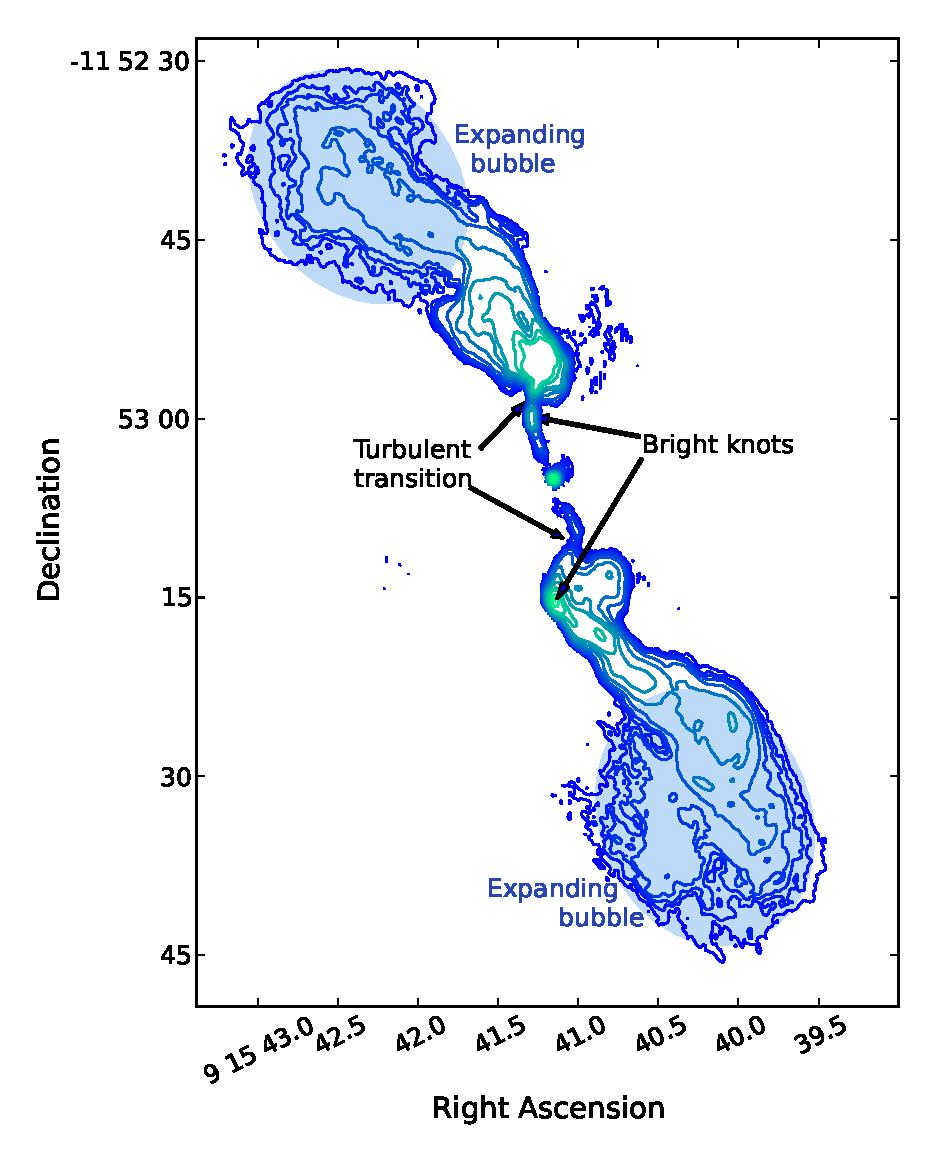
\includegraphics[width=10cm]{taylor.eps}
\caption{ Radio intensity map of Hydra~A at 4.635 GHz. This figure is almost identical to Fig. 1 in \citet{taylor90}. Contour levels are at 1.5, 2.7, 3.7, 5.1, 10, 21, 37, 51, 103, 154, 311, and 466 mJy arcsec$^{-2}$. 
The elliptical areas outline the approximate volume of the corresponding X-ray A and B cavities and are used to estimate the contribution to the jet kinetic power. }
\label{taylor}
\end{figure*}

%\textbf{(b)} Zoom-in of the top rectangular region in a) showing the bright knots in the northern jet. Contours are at 1.5, 2.7, 3.7, 5.1, 6.3, 7.5, 8.8, 10, 21, 37, 51, 72, 90, 103, 154, 311, and 466 mJy arcsec$^{-2}$. \textbf{(c)} Zoom-in of the bottom rectangular region in a) showing the bright knots in the southern jet. Contours are at 1.5, 2.0, 2.2, 2.7, 3.7, 5.1, 5.5, 6.0, 6.3, 6.8, 7.5, 8.8, 10, 21, 37, 51,  72, 90, 103, 154, 311, and 466 mJy arcsec$^{-2}$.



%%%%%%%%%%%%%%%%%%%%
%
% Jet Power from a Shock Model
%
%%%%%%%%%%%%%%%%%%%%
\subsection{Jet power based on a model for the outer shock}\label{s:powsh}

\citet{nulsen05} focused on the outer shock evident in the X-ray image and used a spherically symmetric hydrodynamic model of a point explosion in an initially isothermal and hydrostatic environment to produce theoretical X-ray surface brightness profiles for Hydra~A. Their best fit to the observed X-ray brightness profile gives a shock age $\sim 1.4 \times 10^8 \, \rm Myr$ and an explosion energy $\sim 10^{61} \, \rm erg$. The estimated power of the outburst is $\sim 2 \times 10^{45} \, \rm erg \, s^{-1}$. On the basis of this model, I would associate $10^{45} \> \rm erg \> s^{-1}$ with each jet.

%%%%%%%%%%%%%%%%%%%%
%
% Jet Power from X-ray data
%
%%%%%%%%%%%%%%%%%%%%
\subsection{Jet power based on X-ray cavities}\label{s:powx}

\citet{wise07} used the observations of three pairs of X-ray cavities revealed in \textit{Chandra} images to estimate the power of the Hydra~A jets. The inner cavities A and B correspond to the 4.6~GHz radio lobes \citep{mcnamara00}, the cavities C and D correspond to the middle lobe in the 1.4 GHz radio image \citep{lane04} and the outer cavities E and F correspond to the outer lobes in the 330 MHz image \citep{wise07}. Wise et al. consider that the three cavities on each side are interconnected and use the sum of the enthalpies, $h_{\rm tot}$
\begin{equation}
h_\mathrm{tot}=\gamma p_{\rm lobe}V_{\rm lobe}/(\gamma -1)
\end{equation}
where $\gamma$ is the polytropic index, $p_{\rm lobe}$ is the pressure of the lobe and $V$ is the volume of the cavity, in all cavities to calculate a total outburst energy. From this, the combined jet power is calculated, $P_\mathrm{jet}=4 p_{\rm lobe} V/t_{\rm cav}$, where $t_{\rm cav}$ is the age of each cavity. The average of three different cavity age estimates was used: the time required for the X-ray cavity to reach its present position if moving at the sound speed, the refilling time of the X-ray cavity, and the time required for the X-ray cavity to rise buoyantly to the present position. Assuming pressure equilibrium of the lobes with the atmosphere they obtained powers for the inner and middle lobes of $\sim 2 \times 10^{44} \> \rm erg \> s^{-1}$ and for the outer lobes, $\sim 6 \times 10^{44} \> \rm erg \> s^{-1}$, which gives a combined jet power $\sim 2 \times 10^{45} \> \rm erg \> s^{-1}$. 

The authors find that a power of $1\times10^{45}$ erg s $^{-1}$ for the northern jet is consistent with the supposition that the jet is still filling the outermost of the X-ray cavities at $\sim200$ kpc (the corresponding radio lobe is visible at 330 Mhz) and driving the large-scale shock. An independent estimate of the jet power from the expansion rate of the outermost cavity, assuming a self-similar evolution of the radius of the cavity wall and the large scale shock agrees with their first estimate to within a factor of 2. This value of the jet power $1\times10^{45}$ erg s $^{-1}$ is also consistent with the estimate of the jet power obtained by \citet{nulsen05} noted above. 

\begin{table}
\caption{Parameters for the determination of the lobe minimum energy.} 
\centering
\begin{tabular}{l c c}
 \hline  \hline
 Parameter & Value \\
 \hline 
 Electron spectral index, $a$  &  2.4 \\
 Lorentz factor lower cutoff, $\gamma_1$   &  100                       \\ 
 Lorentz factor upper cutoff, $\gamma_2$ &   10$^6$ \\  
 Central surface brightness, $I_{\nu}$       & 10 mJy arcsec$^{-2}$	 \\ 
 Plasma depth, $L$    & 20 kpc (northern lobe) \\ 
                          & 22 kpc (southern lobe) \\ \hline
\end{tabular}
\label{radio_data}
\end{table}

%%%%%%%%%%%%%%%%%%%%%%%%%


%%%%%%%%%%%%%%%%%%%%
%
% Jet Power from Radio Data
%
%%%%%%%%%%%%%%%%%%%%
%\subsection{Estimates of the power associated with cavities A and B using radio data}\label{s:powr}
\subsection{Estimates of the jet power from synchrotron minimum energy}\label{s:powr}


I revisit the calculation of the cavity powers of the two innermost cavities \citep[see][]{wise07} by using the synchrotron minimum energy estimate for the pressure and synchrotron ages of the lobes. The main difference between this method and that using the X-ray cavities is that the former introduces a strong dependence of the lobe pressure on the particle content of the lobe, whereas the X-ray cavity pressure only depends weakly on the particle content through the adiabatic index. 

The work by \citet{croston05a} on the lobes of classical double (FRII) radio galaxies shows that using a synchrotron minimum energy estimate is a feasible approach. However, since Hydra~A is an FRI source this requires further justification. \citet{croston05a} used observations of the inverse Compton emission in their sample to show that the lobes are close to equipartition when the inverse ratio of energy in relativistic electrons/positrons to that of ``other'' particles, $k=0$. They use this fact to rule out an energetic relativistic proton component since the existence of such a component would imply that the magnetic field is in equipartition with the relativistic electrons only. While the authors did not state this directly, their argument can also be used to exclude an energetic thermal component. This is evident for powerful FRII sources, for which we do not expect much entrainment to occur. However, I argue that the turbulent processes leading to equipartition are independent of the plasma composition and that in the case where the plasma has a substantial thermal content these processes also lead to a minimum energy state between \emph{all} particles and the magnetic field. This conclusion is supported by the work of \citet{birzan08} discussed below.     

I have approximated the shapes of the lobes with ellipsoidal volumes as shown by the shaded elliptical regions in Fig.~\ref{taylor}a; the plasma depth is taken to be equal to the minor axis, $L$. The lobe centres are located at $\sim 30$~kpc from the core. Let $I_\nu$ be the central surface brightness of each lobe, where $\nu=4.6$ GHz is the frequency of the \citet{taylor90} observations. Let $m_{\rm{e}}$ be the electron mass, $e$ the elementary charge, $a$ the electron index, $\alpha=(a-1)/2$ the spectral index, and $\gamma_1$ and $\gamma_2$ the lower and upper cutoff Lorentz factors, respectively. Then, the minimum energy magnetic field (in Gauss) \citep[e.g][]{bicknell13a} of the synchrotron radiating plasma is given by: 

\begin{equation}
B_{\rm{min,E}} = \frac{m_{\rm{e}} c}{e}\left[ \frac{a+1}{2}(1+k)C^{-1}(a)\frac{c}{m_{\rm{e}}}f(a,\gamma_1, \gamma_2)\frac{I_{\nu}\nu^{\alpha}}{L} \right]^{\frac{2}{a+5}}\;,
\label{e:bmin}
\end{equation}
where 
\begin{equation}
f(a, \gamma_1, \gamma_2) = (a-2)^{-1} \gamma_1^{-(a-2)} \left [ 1 - \left( \frac{\gamma_2}{\gamma_1}\right)^{-(a-2)}\right]\:,
\end{equation}
and 
\begin{eqnarray}
C(a) &=& 3^{a/2}2^{-(a+7)/2}\pi^{-(a+3)/2} \nonumber  \\
&& \times  \frac{\Gamma\left(\frac{a}{4}+\frac{19}{12}\right)\Gamma\left(\frac{a}{4}-\frac{1}{12}\right)}{a+1} \> 
\frac{\sqrt{\pi}}{2}\frac{\Gamma\left(\frac{5+a}{4}\right)}{\Gamma \left(\frac{7+a}{4}\right)}\;.\label{eq:ca}
\end{eqnarray}
In Eqn.~\eqref{eq:ca} $\Gamma$ is the Gamma-function. Values adopted for $a$, $\gamma_1$, $\gamma_2$, $I_{\nu}$, and $L$ are shown in Table \ref{radio_data}. I choose a spectral index $\alpha\approx0.7$ (hence $a=2.4$), which is representative of the low frequency spectral index of the radio emission \citep{cotton09}.
I choose a lower Lorentz cutoff $\gamma_1=100$, in view of numerous studies of radio galaxies finding $\gamma\sim100-10^3$  \citep{carilli91,  hardcastle01, godfrey09}. Also, $\gamma_2\approx10^6$, since this corresponds to emission frequencies well above the microwave range. Minimum energy estimates are insensitive to $\gamma_2$ and only weakly dependent on $\gamma_1$.

The minimum total (particles + field) energy density of the lobe is given by 
\begin{equation}
\varepsilon_{\rm{tot}} = \varepsilon_{\rm p} + \frac {B_{\rm min,E }^2}{8 \pi} = \frac{a+5}{a+1}\frac{B_{\rm{min,E}}^2}{8 \pi}\;,
\end{equation}
and the total pressure of the lobe corresponding to the minimum total energy density is
\begin{equation}
p_{\rm{tot}}=\frac{1}{3}\varepsilon_\text{e}(1+k)+\frac{B_\text{min,E}^2}{8 \pi}\:.
\label{total_pressure}
\end{equation}
The major uncertainty in this calculation arises from the lack of observational constraints on the parameter $k$. The value of $k$ determines whether the lobe (in equipartition) is over-pressured or under-pressured with respect to the environment, and later in this section I discuss the range of values for $k$ applicable to the Hydra~A radio lobes. Estimates of $B_{\rm{min,E}}$ and $p_{\rm{tot}}$ are given in Table \ref{minimum_energy} for three values of $k$. 

I estimate the age of the source from the curvature in the spectrum derived by \citet{cotton09} who showed that the spectra of the inner lobes steepen for frequencies $\geq 300 \> \rm MHz$. Let $B=B_\mathrm{min,E}$ be the minimum energy magnetic field and $\nu_{\rm{b}} \approx 300 \> \rm MHz$ be the break frequency, then the synchrotron age of the source is 
\begin{equation}
t_{\rm{rad}} \approx \frac{3^{5/2}}{8 {\pi}^{1/2}} \left(\frac{m_e^3 c^5}{e^3}\right)^{1/2} B^{-3/2}\nu_{\rm{b}}^{-1/2}\:.
\end{equation}
Hence, the power associated with each of the inner cavities is 
\begin{equation}
P_{\rm cav} = \frac{\gamma}{(\gamma -1)} \frac{p_{\rm lobe} V_{\rm lobe}}{t_{\rm rad}}.
\label{p_cav}
\end{equation}
I use the total pressure $p_{\rm{tot}}$ for minimum energy conditions as the lobe pressure. Values of $P_{\rm{cav}}$ for different values of $k$ are given in Table \ref{minimum_energy}.



%%%%%%%%%%%%%%%%%%%%%%%
%
%	Table: jet_parameters
%
%%%%%%%%%%%%%%%%%%%%%%% 


\begin{table*}
\caption{Parameters calculated for three values of $k$ using synchrotron minimum energy for both lobes of Hydra A. }
\label{minimum_energy}
\centering
\begin{threeparttable}
\begin{tabular}{*{7}{c}}
\hline \hline
   $k$ & $B_{\rm{min,E}}$  & $\varepsilon_{\rm{tot}}$  & $p_{\rm{tot}}$ &  $p_{\rm{tot}}/p_{\rm{a}}$ & $P_{\rm{cav}}$ & $t_{\rm{rad}}$    \\
       & (10$^{-6}$ Gauss)  & ($10^{-10}$ erg cm$^{-3}$) &  ($10^{-10}$ dyne cm${^{-1}}$) & & ($10^{44}$ erg s$^{-1}$) & (Myr)  \\ 
             \multicolumn{7}{c}{Northern Lobe} \\ \hline
%           &  \multicolumn{7}{c}{\it Electrons + non-relativistic particles} \\ 
  0 & 22 & 0.4 & 0.3  & 0.2 & 0.1 & 49  \\ 
  10 & 42 & 1.5 & 1.2 & 0.9 &  1.8 &  18 \\ 
  100 & 76 & 4.9 &  3.9 & 3.0 & 14.5  & 7  \\
%           &  \multicolumn{7}{c}{\it Electrons + relativistic particles} \\ 
%  0 & 22 & 0.4 & 0.3  & 0.1 &  0.1 & 32 & 0.1 & 49  \\ 
%  10 & 42 & 1.5 & 1.2 & 0.6 &  1.0 & 14  & 1.3 & 18 \\ 
%  100 & 76 & 4.9 &  3.9 & 2.0 &  6.0 & 8 & 15.4 & 7  \\
  \hline
   \multicolumn{7}{c}{Southern Lobe} \\ \hline
       0 &  21 & 0.4 & 0.3 & 0.2 &  0.1  & 51 \\
       10 & 40 & 1.4 & 1.1 &  0.9 &  2.0 & 19 \\ 
       100 & 73 & 4.6 & 3.7 & 3.0 &  16.3   & 8 \\
\hline
\end{tabular}
\end{threeparttable}
\end{table*}


Table \ref{minimum_energy} shows, for both the northern and southern lobes, the estimation of the minimum energy magnetic field, $B_{\rm{min,E}}$, the total energy density $\varepsilon_{\rm tot}$, the total pressure of the lobe, $p_{\rm{tot}}$, the ratio between the total lobe pressure and the atmospheric pressure $p_{\rm{tot}}/p_{\rm{a}}$, the cavity power for $\gamma = 4/3$, and the radiative ages of the lobes for values of the parameter $k=0, \ 10 \rm \ and \ 100$.

For the same value of $k$, the cavity powers of the northern and southern lobes are comparable. Moreover, for $k=10$ the lobes are in approximate pressure equilibrium with the atmosphere and the cavity powers ($1.8 \times 10^{44}$ and $2.0\times 10^{44} \> \rm ergs \> s^{-1}$ respectively) agree with the \citet{wise07} estimates of $2.1\times 10^{44} \> \rm ergs \> s^{-1}$ and $2.0\times 10^{44} \> \rm ergs \> s^{-1}$ respectively. For $k=0$ the lobes appear to be significantly under-pressured and for $k=100$ significantly over-pressured.

This high value of $k$, i.e., energy dominated by the heavy particles, is  supported by a recent study performed by \citep{birzan08}. They estimate $k$ for a group of galaxies including Hydra A assuming pressure equilibrium between the radio lobe and the atmosphere. For the 1.4GHz inner lobe of Hydra A they obtained a value of $k\approx13$. In their study of the inverse-Compton X-ray emission of the outer lobe of Hydra A \citet{hardcastle10} estimates a moderate value of $k=17 - 23$. 

The major uncertainty associated with these radio-based estimates of the cavity power is that there is no direct estimate of the lobe pressure and I have assumed that the lobe pressure is determined by the total pressure of the lobe when the lobe is in its minimum energy state. This assumption gives a lower limit of the lobe energy, and hence a lower limit on the cavity power.


The estimation of the power associated with the inner radio lobes and the power of the corresponding X-ray cavities given in \S~\ref{s:powx} for a nearly pressure equilibrium situation are consistent. This indicates the total jet power obtained by summing the powers of all X-ray cavities presented presented by \citet{wise07} is reliable and provides a sound basis for numerical models of Hydra A.  
I therefore adopt a jet power of $10^{45} \> \rm erg \> s^{-1}$ as our value in the simulations presented in \S~\ref{s:sims}. 

% with the cavity power estimates for the northern and southern lobes respectively. 
%This indicates that the result for the total jet power from the summation of all cavity powers, obtained by \citet{wise07} is reliable and provides a sound basis for numerical models of Hydra A. 

%%%%%%%%%%%%%%%%%%%%%%%%%%%%%%%%%%%%%%%%%%%%
%
%					Cluster Environment
%
%%%%%%%%%%%%%%%%%%%%%%%%%%%%%%%%%%%%%%%%%%%%
\section{Cluster Environment} \label{s:cluster}
 

\begin{figure}
\centering
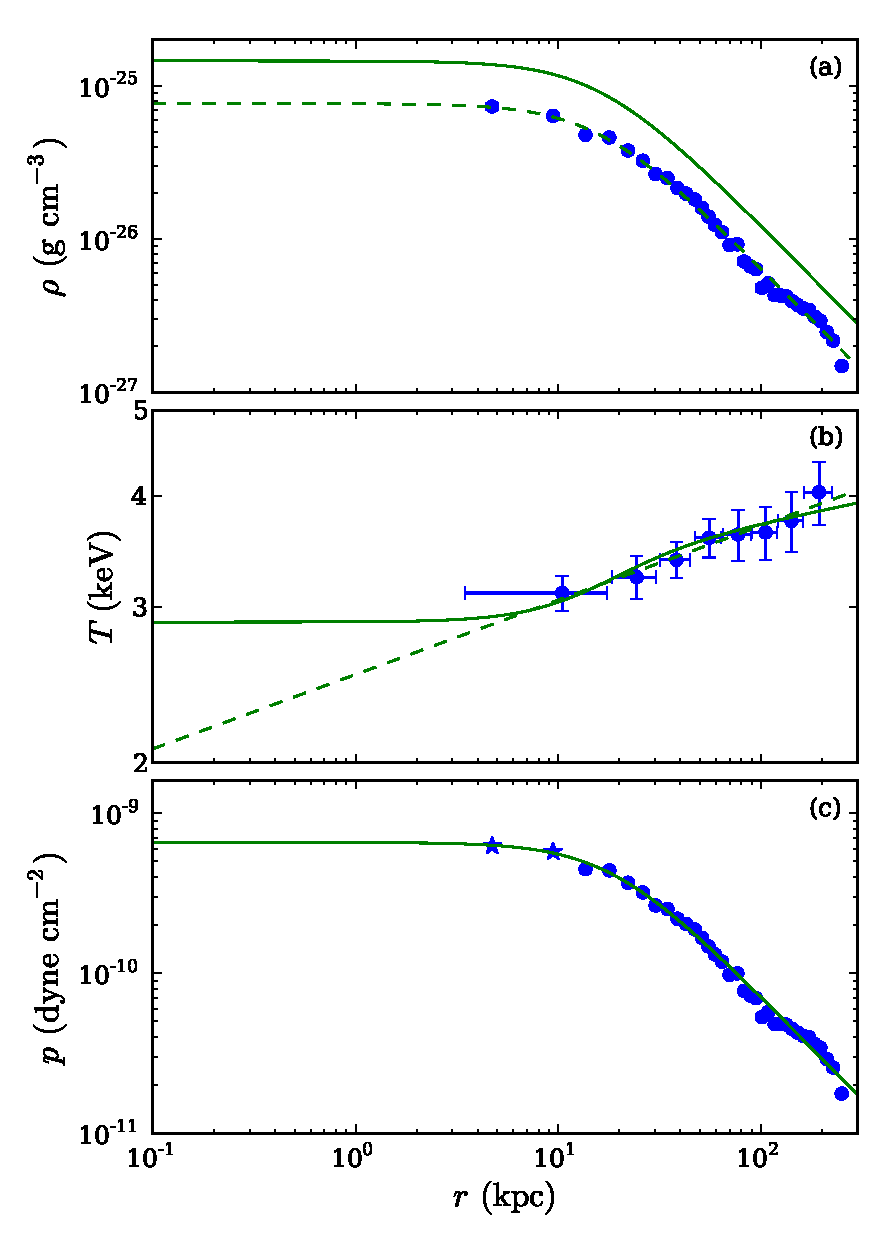
\includegraphics[width=130mm]{ICM.eps}
\caption{Radial thermodynamic profiles for the Hydra A galaxy cluster. \textbf{(a)} Electron density (data points and dashed line), and corresponding total particle density (solid line) assuming a fully ionized plasma; Error bars are smaller than the points. \textbf{(b)} Electron temperature (data points and dashed line) and the temperature profile obtained from the total particle density and the pressure profiles (solid line); \textbf{(c)} Total pressure. The points in (a) and (b) are data for the electron density and electron temperature, respectively, obtained by \citet{david01} from X-ray observations of the Hydra A atmosphere. The dashed curves are fits to the data points using Eqn~\ref{density_profile} for (a) and a power-law for (b). The points in (c) were calculated from the density data points and the temperature fit. The stars represent the additional data points that I obtained through this method inside of 10 kpc. These two data points are important in constraining the profiles in the innermost region. The line in (c) is a fit to the data with Eqn.~\eqref{pressure_profile}.
Finally the temperature profile (solid line in panel b)) is obtained from the total particle density and the pressure profile. \newline
(A colour version of this figure is available in the online journal)}
\label{profiles}
\end{figure}


\begin{table}
\caption{Atmosphere profile parameters. Fits to data by \citet{david01} and extrapolation to $r<10$ kpc.} 
\centering
\begin{tabular}{r c c}
 \hline\hline
 & Parameter & Best fit value \\
 \hline
 \multirow{3}{*}{Density profile} & $r_{\rho 0}$ &  15.94 kpc \\
 & $\rho_0$     &  $1.49\times 10^{-25}$ g cm$^{-3}$ \\
 & $\alpha_{\rho}$ & 0.67  \\  
 \hline
 \multirow{2}{*}{Temperature profile} & $a_T$   & 5.66     \\
 & $b_T$   & $8.4\times10^{-2}$ \\
 \hline
 \multirow{3}{*}{Pressure profile} & $r_{p0}$  & 18.21 kpc	 \\
 & $p_0$     &	$6.58 \times 10^{-10}$ dyne cm$^{-2}$ \\
 & $\alpha_{p}$ & 0.65  \\
 \hline
\end{tabular}
\label{halo parameters}
\end{table}


In order to construct definitive simulations of the inner jet propagation, I require knowledge of the distribution of the ambient density and pressure on a 10~kpc scale. In this section I present useful analytical fits for the density, temperature, and pressure in the cluster environment, which I use to estimate the pressure and density in the inner 10 kpc.

I assume that Hydra A's atmosphere prior to the passage of the jet is hydrostatic, following a spherically-symmetric density distribution of the form
\begin{equation}
\rho(r) = \frac{\rho_0}{(1+r^2/r_{\rho0}^2)^{\alpha_{\rho}}}\:.
\label{density_profile}
\end{equation}
$\rho_0$, $r_{\rho0}$, and $\alpha_{\rho}$ are determined through a least-squares fit of the function given in Eqn.~\eqref{density_profile} to the models for the cluster density inferred from the X-ray surface brightness by \citet{david01}. The data and the fitted density profile are shown in Fig.~\ref{profiles} a). The pressure distribution of the atmosphere depends on the temperature distribution through 
\begin{equation}
p = \rho k_B T/\mu m
\end{equation}
 where $k_B$ is Boltzmann's constant, $\mu$ is the molecular weight and $m$ is the atomic mass unit. However, there is no observational data for the temperature inside of 10 kpc. I therefore use a power law temperature fit, $\log T = a_T+b_T\log r$, as shown in Fig.~\ref{profiles} b), to the \citet{david01} data and the density profile given by Eqn.~\eqref{density_profile} to obtain corresponding pressure values for two additional points within a radius of 10 kpc; these are distinguished from the other data points by the star-shaped symbols in Fig.~\ref{pressure_profile} c). The two additional extrapolated data points are important in constraining the shape of the flattening pressure profile toward the core of the galaxy. I adopt the following analytic expression for the pressure profile of the ICM
\begin{equation}
p(r) = \frac{p_0}{(1+r^2/r_{p0}^2)^{\alpha_p}}\:.
\label{pressure_profile}
\end{equation}
A least squares fit to the pressure data points is used to obtain the parameters  $p_0$, $r_{p0}$, and $\alpha_p$.  
 We then obtain the final temperature fit (solid line in panel b)) using the total particle density (solid line in panel a)) and the pressure profile (solid line in panel c)). 
 The best-fit parameters for the fits to the density, temperature, and pressure data are summarised in Table \ref{halo parameters}. 

For a hydrostatic environment I now have a gravitational acceleration profile
\begin{equation}
g(r) = - \frac {1}{\rho} \frac {dp}{dr} =  -2\alpha_p \frac{p_0}{\rho_0} \frac{r}{r_{p0}}\frac{(1+r^2/r_{\rho0}^2)^{\alpha_{\rho}}}{(1+r^2/r_{p0}^2)^{1+\alpha_p}}\:.
\end{equation}


\chapter{Jet model based on a single knot}\label{chapter4}
\begin{figure}
\centering
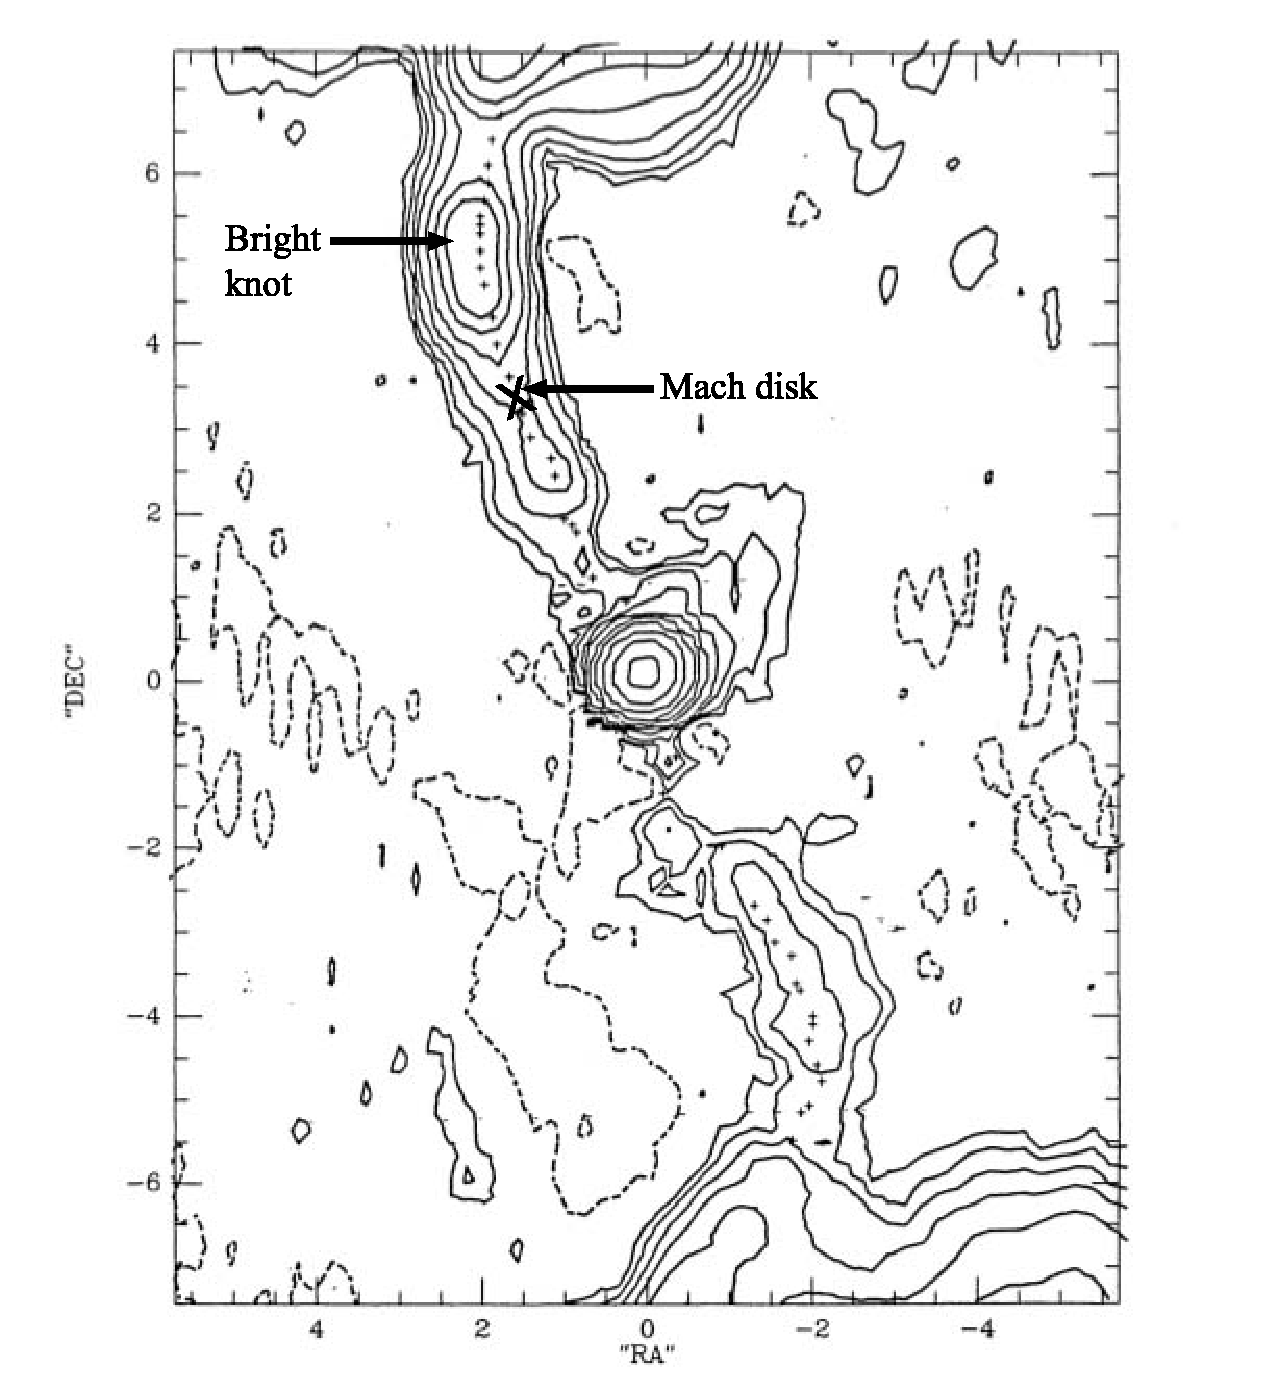
\includegraphics[width=\linewidth]{tp.eps}
\caption{Fig. 3 of \citet{taylor90}. Central 10~kpc jets of Hydra A. Contour levels are at 1.0, 2.0, 7.8, 15, 32, 51, 103, 208, and 417 mJy arc sec$^{-2}$. The bright knot is marked with black arrow. The location of the Mach disk (at approximately 6~kpc, marked by a $\times$) which I originally interpret as the reason for the bright knot, is also indicated.}
\label{f:morph}
\end{figure}

\begin{figure}
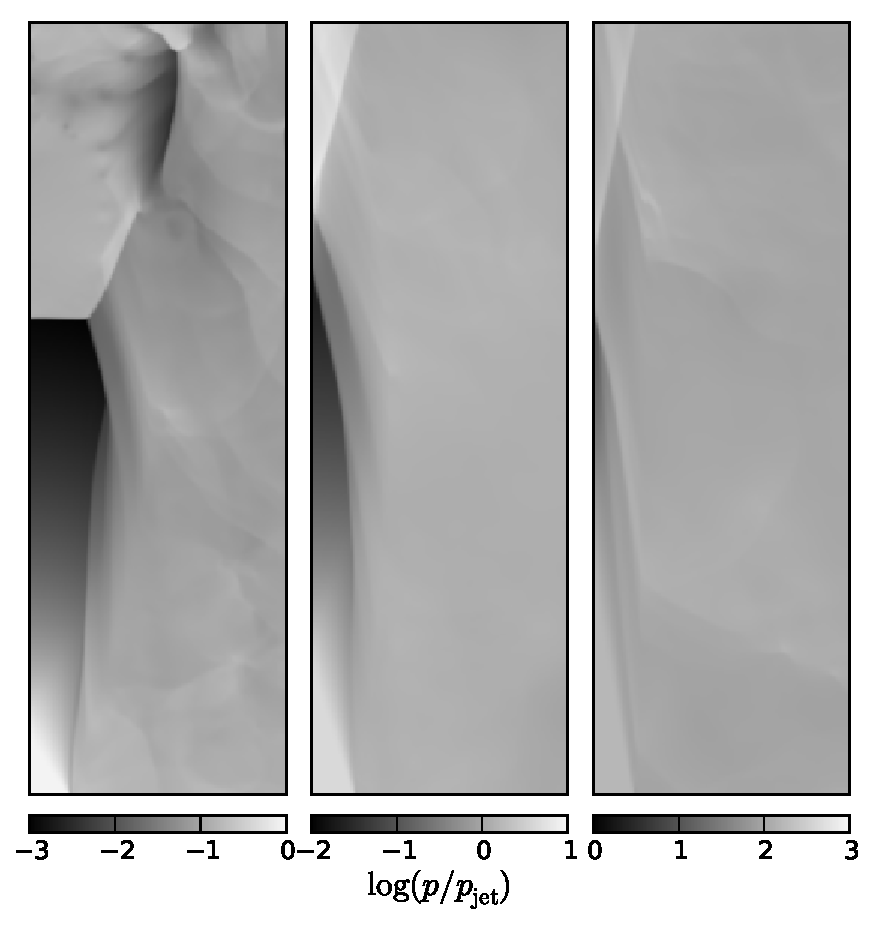
\includegraphics[width=\linewidth]{pss.eps}
\caption{Logarithmic pressure maps of the jet and ambient medium in the inner region of the 2D simulations. Left: A jet with an over-pressure ratio of 10 producing a Mach disk (Simulation Cvia). Middle: A jet with an over-pressure ratio of 5 producing a reconfinement shock. (Simulation Cviib) Right: A nearly pressure equilibrium jet ($p_{\rm jet}/p_{\rm a} = 2$) producing a very weak conical reconfinement shock (Simulation Cviic). Each panel has physical dimensions of $2\,\mathrm{kpc}\times6\,\mathrm{kpc}$.}
\label{pressure_comparison}
\end{figure}

%The first goal of this thesis is to understand the physics involved in the jet-ICM interaction within the central 10~kpc of the source Hydra A.  

My initial work on modelling Hydra A was based upon the published images of \citep{taylor90} in which a single bright knot is evident in the first 10~kpc of the northern jet. Consequently the work described here is based upon the production of a single bright knot in the first 10 kpc. Subsequent to this work, Prof, Gregory Taylor kindly provided a FITS image of Hydra A so that I could determine the brightness ratio of the northern and southern jets. When I contoured this image I realised that there are in fact two knots in the northern Hydra A jet (see Fig.~\ref{taylor}), first of which could with hindsight be faintly discerned in the original published images. Consequently, the following chapter contains a series of models devoted to the modelling of two knots. This chapter describes my work on the single knot interpretation. The comparison between the two models is of interest since it shows the different parameters that are obtained when different assumptions are made. 

%% Modify the following text to be consistent.
%I first focus the bright knot apparent at approximately 6 to 10~kpc of the northern jet (see Fig.3 of \citet{taylor90}). 
%Fig.~\ref{taylor} is produce later from the original 6~cm VLA data kindly provided by Professor Gregory Taylor which shows two inner knots at approximately 3.7~kpc and 7.0~kpc in the northern jet until it becomes turbulent. Therefore, the study presented in this chapter only consider the second knot. Moreover looking at Fig.3 of \citet{taylor90} I assume the southern edge of the second knot is at $\sim$6~kpc away from the black hole. 

My initial guess is that the bright knot in the northern jet is a consequence of a Mach disk at approximately 6~kpc produced by the interaction of an over pressured jet and the cluster environment. See \S~\ref{sec:reconf} for the description of reconfinement shock model of jet knots. Depending on the pressure ratio between the jet and the atmosphere, there are two different types of reconfinement shock structures that can occur: strong shocks perpendicular to the jet flow, often referred to as Mach disks, and conical shocks. Fig.~\ref{pressure_comparison} shows a comparison of the morphology of a jet that is significantly over-pressured (left panel), mildly over-pressured, and in nearly pressure equilibrium (right panel) with respect to the ambient medium. It is well known that a supersonic jet may display a sequence of conical shocks, also known as ``diamond shocks'', if the jet is over or under-pressured or in nearly pressure-equilibrium with respect to the ambient medium. The jet repeatedly expands and contracts towards the jet axis resulting in a sequence of conical shocks. When the pressure ratio of the jet and the atmosphere is sufficiently high (e.g., $p_{\rm{jet}}/p_{\rm{a}}\gtrsim10$), a Mach disk occurs normal to the flow. Such shocks occur in the following way: The propagation of the supersonic jet produces a lobe of shocked gas whose pressure is initially higher than the jet pressure. As the jet propagates, the lobe pressure decreases. When the lobe pressure becomes lower than the jet pressure, the jet expands rapidly sideways and the subsequent reconfinement produces a Mach disk. Behind the Mach disk, a transition to turbulence occurs, which is more rapid than that associated with conical shocks. A Mach disk is very disruptive; it drastically reduces the jet velocity in the inner section of the jet and also establishes a strongly sheared flow between the inner jet and its outer layer as shown in Fig. \ref{f:morph}. Oblique conical shocks are not as disruptive as the Mach disk. 

%\citet{norman82} first drew attention to the production of conical and normal shocks in over-pressured astrophysical jets.

%%%%%%%%%%%%%%%%%%%%%%%%%%%%%%%%%%%%%%%%%%%%%%%%%%%%%%%%%%%%%%%%%%%%%%%%
%
%												CODE AND SIMULATION PARAMETERS
%
%%%%%%%%%%%%%%%%%%%%%%%%%%%%%%%%%%%%%%%%%%%%%%%%%%%%%%%%%%%%%%%%%%%%%%%%
\section{Simulation Parameters} \label{code}

%%%%%%%%%% new table %%%%%%%%%%%%%4
\begin{table*}
%\begin{sidewaystable}
\caption{Simulation parameters. In all simulations, $r_{\rm{jet}}=0.38$ kpc.}
\centering
\begin{tabular}{l * {8}{c}}
\hline \hline
Model  & $p_{\rm{jet}}/p_{\rm{a}}$ & $\beta$ & $\chi$ & $\eta$ & $\phi$ (rad cm$^{-2}$) & $\Psi_{6\rm{cm}}$ (rad) & $\Psi_{20\rm{cm}}$ (rad) \\
\hline
    %%%%%%%%%% 		set A 	%%%%%%%%%%%%%%%
	\multicolumn{8}{c}{Set A, $P_{\rm{jet}}=1\times10^{45}$ erg s$^{-1}$} \\ 
	\hline
  	 Ai		&  10 & 0.09 & 1029 & $1.2\times10^{-1}$ &	$3.2\times10^{-2}$ 			&	1.14	 		&	12.63  \\
	Aii 	&  10 & 0.11 &  530  &  $6.0\times10^{-2}$ &	$1.6\times10^{-2}$	 		&	0.59	 		& 6.51	 \\
	Aii	&  10 & 0.13 &   301 & $3.4\times10^{-2}$ &	$9.2\times10^{-3}$ 	 		&	0.33 	 		&   3.69	 \\
	Aiv	&  10 &  0.15 &  182 & $2.0\times10^{-2}$ &	$5.6\times10^{-3}$			&	0.20	 		& 	2.23	\\
	Av	&  10 & 0.17 &  116 & $1.3\times10^{-2}$  &	$3.6\times10^{-3}$	  		&	0.13			&  1.42	\\
	Avi 	&  10 &  0.19   &    76 &  $8.5\times10^{-3}$ &	$2.3\times10^{-3}$ 			& 0.08	  		& 0.93 \\
	Avii	&  10 &  0.21   &    51 &  $5.7\times10^{-3}$ &	$1.6\times10^{-3}$			&   0.06			& 0.63	 \\
	\hline
	%%%%%%%%%% 		set B 	%%%%%%%%%%%%%%%
	\multicolumn{8}{c}{Set B, $P_{\rm{jet}}=3\times10^{44}$ erg s$^{-1}$} \\ 
	\hline 
	Bi	&10 & 0.04 & 3143  & $3.5\times10^{-1}$	&	$9.7\times10^{-2}$			& 3.47	 	& 38.59 \\
	Bii 	&  10 & 0.05 &   1447 & 	$1.6\times10^{-1}$ &	$4.4\times10^{-2}$	 	& 1.60	 	& 17.76	\\
	Biii	&  10 & 0.06 &   743 &  	$8.3\times10^{-2}$	& $2.3\times10^{-2}$		& 0.82	 	& 9.12	 \\
	Biv	& 10 &  0.07 &  409 &  	$4.6\times10^{-2}$	& $1.3\times10^{-2}$	 	& 0.45	 	& 5.02	  \\
	Bv	& 10 & 0.08 &  234 & 	$2.6\times10^{-2}$	&	 $7.2\times10^{-3}$ 		&	0.25	 	& 	2.87	 \\
	Bvi	&  10 &  0.09   &   136  &  $1.5\times10^{-2}$	& $4.2\times10^{-3}$	 	&	0.15	  	& 1.67	 \\
	Bvii	&  10 &  0.10   &    79 &   $8.8\times10^{-3}$	& $2.4\times10^{-3}$ 		& 	0.09	  	& 	0.97	 \\
	\hline
%\begin{comment}
	%%%%%%%%%% 		set C 	%%%%%%%%%%%%%%%
        \multicolumn{8}{c}{Set C, $P_{\rm{jet}}=3\times10^{45}$ erg s$^{-1}$} \\
        \hline
	Cia	&10 & 0.25 & 135 & $1.5\times10^{-2}$  & 	$4.1\times10^{-3}$			&	0.15		 	& 	1.66	 \\
	
   Cib  &5 & 0.25 & 301 & $1.7\times10^{-2}$  	&	$4.6\times10^{-3}$ 	   			&	0.17	 		& 	1.85		\\
   Cic  &2 & 0.25 & 800 & $1.8\times10^{-2}$   	&	$4.9\times10^{-3}$	 			&	0.18	  		&	1.96		\\	
    
	Ciia 	& 10 & 0.30 &  71 &  $7.9\times10^{-3}$ 	& $2.2\times10^{-3}$	 		&	0.08	 		& 0.87 	  	\\
    
    Ciib    &5 & 0.30 & 164 & $9.1\times10^{-2}$  & $2.5\times10^{-3}$ 	  			&	0.09	 		& 1.01	 \\
    Ciic    &2 & 0.30 & 442 & $1.0\times10^{-3}$  	&	$2.7\times10^{-3}$    		&	0.10		& 1.09	 \\

	Ciiia 	& 10 & 0.35 &  40 &  $4.5\times10^{-3}$  	& $1.2\times10^{-3}$	 		&	0.04			& 0.49  \\

   Ciiib    &5 & 0.35 & 96 & $5.4\times10^{-2}$ 	&	$1.5\times10^{-3}$ 	   			&	0.05			&	0.59		\\
    Ciiic   &2 & 0.35 & 263 & $5.9\times10^{-3}$   &	$1.6\times10^{-3}$ 	 			&	0.06	  		& 0.64		\\

	Civa	& 10 &  0.40 & 23 & $2.6\times10^{-3}$ 	& $7.2\times10^{-4}$			&	0.03	    	& 0.29	 \\

    Civb    &5 & 0.40 & 59 & $3.3\times10^{-2}$  	& $9.0\times10^{-4}$	   		&	0.03		& 0.36	 \\
    Civc  &2 & 0.40 & 165 & $3.7\times10^{-3}$   	& $1.0\times10^{-3}$	  		&	0.04	 	& 0.41	 \\

	Cva 	& 10 & 0.45 &  14 & $1.6\times10^{-3}$	& $4.3\times10^{-4}$	 		&	0.02   	&	0.17   \\

    Cvb    &5 & 0.45 & 37 & $2.1\times10^{-2}$   	& $5.7\times10^{-4}$	 		&	0.02  	&	 0.23 \\
    Cvc   &2 & 0.45 & 107 & $2.4\times10^{-3}$  	& $6.6\times10^{-4}$	 		&	0.02  	& 0.26	 \\

	Cvia & 10 & 0.50 & 8 &  $9.3\times10^{-3}$ 	& $2.6\times10^{-4}$	 		&	0.01	 	& 0.10	 \\

  Cvib    &5 & 0.50 & 24 & $1.4\times10^{-2}$   	&  $3.7\times10^{-4}$	 		&	0.01 		&	0.15	 \\
   Cvic    &2 & 0.50 & 71 & $1.6\times10^{-3}$   	& $4.4\times10^{-4}$	  		&	0.02	 	& 0.18	 \\

	Cviia	& 10 & 0.55 & 5 & $5.3\times10^{-4}$ 	& $1.5\times10^{-4}$	 		&	0.01  	& 0.06	 \\

   Cviib   &5 & 0.55 & 16 & $8.7\times10^{-4}$  	& $2.4\times10^{-4}$	   		&	0.01  	&	 0.10 \\
   Cviic   &2 & 0.55 & 48 & $1.1\times10^{-3}$  	& $3.0\times10^{-4}$	 		&	0.01  	& 0.12 		\\
\hline
	
%\tablefootnote{index $p$ is used to separate the parallel opening jet models presented here and the conically expanding jet models presented in the following chapter.}
\end{tabular}
\label{simulation_parameters}
%\end{sidewaystable}
\end{table*}



%%%%%%%%%%%%%%%%%%%%%%%%%%%%%%%

%\begin{table*}
\begin{sidewaystable}
\caption{Inferred jet velocities for Hydra A northern jet as a function of jet power and pressure ratio}
\begin{tabular}{l * {16}{c}}
\hline \hline
$P_{\rm{jet}}$(erg s$^{-1}$) & $p_{\rm{jet}}/p_{\rm{a}}$  & $\chi$ & $\eta$ & $\beta$ \\
\hline
 $3\times10^{44}$ & 10 & 1447 & $1.6\times10^{-1}$ & 0.05 \\ 
 $1\times10^{45}$ & 10 &  116 & $1.3\times10^{-2}$   & 0.17 \\ 
 $3\times10^{45}$ & 10 &   14 & $1.6\times10^{-3}$ & 0.45 \\ 
 $3\times10^{45}$ &  5 &   59, 37, 24, 16 & $(3.3, 2.1, 1.4, 0.1)\times10^{-2}$ & 0.4-0.55 \\ 
  $3\times10^{45}$ &  2 &   800, 442, 263, 165, 107, 71, 48  & $(1.8, 0.1, 0.6, 0.4, 0.2, 0.2, 0.1)\times10^{-2}$ & 0.25-0.55 \\ 
\end{tabular}
\label{inferred_jet_velocities}
\end{sidewaystable}
%\end{table*}


%For the simulations I use the the publicly available PLUTO code \citep{mignone07} to calculate two dimensional axisymmetric hydrodynamic models of the jet-ICM interaction in Hydra A. Since some of the models include relativistic velocities I use the relativistic hydrodynamic (RHD) module available in PLUTO. 

In the models presented here, I initialise a parallel jet into the computation domain following \citet{sutherland07, wagner11}.  The $(r, z)$ computational domain for the two dimensional axisymmetric simulations is a cylinder of radius $r=25$ kpc and height $z=50$ kpc. Using a stretched grid I define a high resolution grid ($1600 \times 160$ cells) within the central $20\,\mathrm{kpc}\times2\,\mathrm{kpc}$ region, giving us 30 cells across the jet, and a lower resolution in the outer regions. I impose an axisymmetric boundary condition for the boundary $r=0$, and a reflective boundary condition for $z=1$.  The remaining boundaries are set to outflowing boundaries.

The jet is initiated within a quarter circle with radius 0.38 kpc and centre at $(r, z) = (0, 1)~kpc$. The time invariant jet parameters are jet power $P_{\rm{jet}}$, jet radius $r_{\rm{jet}}$, inlet jet pressure $p_{\rm{jet}}$, inlet jet velocity $\beta$, and the proper density parameter 
\begin{equation}
\chi =  \frac{\rho_{\rm jet} c^2}{\varepsilon + p_{\rm jet}} = (\gamma -1)\rho_{\rm{jet}}c^2/\gamma p_{\rm{jet}}
\end{equation}
where $c$ is the speed of light, $\varepsilon$ is the internal energy density, and $\gamma$ is the polytropic index. The jet velocity vectors at the jet base are parallel to the positive $z$--direction.
%$\chi = (\gamma -1)\rho_{\rm{jet}}c^2/\gamma p_{\rm{jet}}$, where $\gamma$ is the polytropic index. The jet velocity vectors at the jet base are parallel to the positive $z$--direction.

%I use the \citet{taub1948a} equation of state, a quadratic approximation to the exact Synge--J\"{u}ttner relativistic perfect gas equation of state \citep{juttner1911a,synge1957a}, which yields $\gamma\rightarrow5/3$ in the low temperature limit, and $\gamma\rightarrow4/3$ in the high temperature limit. Because the radiative cooling time of the ambient gas and the synchrotron cooling time of the jet plasma is large compared to the simulation time (which is equivalent to the jet crossing time), I do not include radiative cooling in the simulations.

Let $A_{\rm{jet}}(=\pi r^2_{\rm{jet}}$) be the jet cross-sectional area and $\Gamma=(1-\beta^2)^{-1/2}$ be the jet Lorentz factor. Then the jet kinetic power is given by \citet{sutherland07}:
\begin{equation}
P_{\rm{jet}} = \frac{\gamma}{\gamma -1} c p_{\rm{jet}}\Gamma^2\beta A_\mathrm{jet}\left(1+\frac{\Gamma -1}{\Gamma}\chi\right)\:.
\label{jet_power}
\end{equation}
We determine the density parameter by solving Eqn.~\eqref{jet_power}:
\begin{equation}
\chi = \frac{\Gamma}{\Gamma -1}\left( \frac{\gamma-1}{\gamma}\frac{P_{\rm{jet}}}{c p_{\rm{jet}} \Gamma^2\beta A_{\rm{jet}}} -1 \right)\:.
\label{chi2}
\end{equation}

The initial conditions for the ambient medium representing the hot ICM surrounding Hydra A are the hydrostatic thermodynamic profiles found in \S~\ref{s:cluster}. The ratio, $\eta =\rho_{\rm jet}/\rho_{\rm  a}$, of the jet to ambient density is always an important parameter in jet theory and since I am allowing for a significant thermal component in the simulations it is important to estimate this parameter. If $T$ is the core temperature of the cluster atmosphere, $\rho_{\rm a}$ and $p_{\rm a}$ are the ambient density and pressure at the jet inlet, $k_B$ the Boltzmann constant and $m$ be the atomic mass unit, $\eta$ is given by 
\begin{equation}
\eta = \frac{\rho_{\rm{jet}}}{\rho_{\rm{a}}} = \chi \frac{\gamma}{\gamma-1}\frac{p_{\rm{jet}}}{p_{\rm{a}}}\frac{k_BT}{\mu m c^2}\:.
\label{eta}
\end{equation}
Equation~(\ref{chi2}) for $\chi$ and equation~(\ref{eta}) for $\eta$ typically lead to values of $\chi \gg 1$ (especially for low velocities) and correspondingly large values of $\eta \approx 10^{-2}$ in comparison to the typical value for AGN jets ($\eta \approx 10^{-4}$). The implications of this are discussed further below.

The simulations presented in the next section cover an extensive region in parameter space. The simulation parameters that are varied, and the ranges they span are: the jet power, $P_\mathrm{jet}=1\times10^{45}$, $3\times10^{44}$, $3\times10^{45} \> \rm erg \> s^{-1}$, the ratio of the jet pressure to that of the atmosphere at the jet base $p_{\rm{jet}}/p_{\rm{a}}=2, 5, 10$, and the jet velocity in units of the speed of light $\beta=0.04 - 0.55 \> c$, are presented in Table \ref{simulation_parameters}. The range in jet velocity is restricted to fairly low values because of the results presented in \S~\ref{s:sims}: the location of the first internal jet shock constrains the velocity to relatively low values. 

%In the model names I use an index $p$ (p for parallel opening jet) to separate the models for the conically expanding jets presented in the subsequent chapter. 

The jet radius is fixed at $r_\mathrm{jet}=0.38$ kpc. This value is measured from the deconvolved FWHM at approximately 1~kpc from the core of the northern jet. Some derived parameters, namely the density parameter $\chi$, the density ratio $\eta$ of the jet and the atmosphere at the jet base, the rotation measure (RM) $\phi$, and the Faraday rotation angle $\Psi$ at 6 cm ($\Psi_\mathrm{6cm}$) and 20 cm ($\Psi_\mathrm{20cm}$) are also presented in Table \ref{simulation_parameters}. The rotation measure and Faraday rotation of the central jet with electron density $n_\mathrm{\mathrm e,jet}$(=$\rho_{\mathrm jet}$(1 + 2 $n_{\mathrm He}$/$n_{\mathrm H}$)/u(1 + 4$n_{\mathrm He}$/$n_{\mathrm H}$), where $u$ is an atomic mass unit), magnetic field along the line of sight $B_z$ (we use $35 \> \mu\,\mathrm{G}$, approximately the minimum energy magnetic field near the jet base), differential plasma depth $dl$, jet radius $R_{\rm{jet}}$, total plasma depth $L=2R_{\rm{jet}}$, and wavelength $\lambda$ are calculated from
\begin{eqnarray}
\phi &=& 8.1\int n_\mathrm{e,jet} B_z dl \quad \rm rad \, cm^{-2} \nonumber \\
&=& 8.1\times10^{-5}\, \left(n_{e, jet}\right) \left(\frac{B_z}{\mathrm{\mu G}}\right)  \left(\frac{2R_{\rm{jet}}}{\mathrm{kpc}} \right) \rm rad \, cm^{-2}
\end{eqnarray}
where the units of $B_z$ and $l$ are Gauss and cm, respectively. The total Faraday rotation through the jet is given by:
\begin{equation}
\Psi_{\rm rad} = \phi \lambda^2 \:.
\end{equation}

%The rotation measure and Faraday rotation angle of the central jet with electron density $n_\mathrm{e,jet}$, ambient electron density $n_\mathrm{e,a}=0.07$ (estimated from the ICM density profile), magnetic field along the line of sight $B_\parallel$ (we use $60 \> \mu\,\mathrm{G}$, approximately the minimum energy magnetic field near  the jet base),
%differential plasma depth $dl$, jet radius $R_{\rm{jet}}$, total plasma depth $L=2R_{\rm{jet}}$, and wavelength $\lambda$ are calculated from
%\begin{eqnarray}
%\phi_{\rm rad \, cm^{-2}} &=& 81 \int n_\mathrm{e,jet} B_z dl \nonumber \\
%&=& 0.081\,n_\mathrm{e,a} \left(\frac{\eta}{10^{-2}}\right) \left(\frac{B_z}{10^{-5}\,\mathrm{G}}\right)  \left(\frac{2R_{\rm{jet}}}{\mathrm{kpc}} \right) \: 
%\end{eqnarray}
%and
%\begin{equation}
%\Psi_{\rm rad} = \phi \lambda^2 \:.
%\end{equation}



I calculate these quantities as an additional check to ensure that the jet parameters are consistent with the fact that the jets are polarised along their length. The internal Faraday rotation should be much less than unity for consistency between the models and the observations. Note however, that the values given in Table~\ref{simulation_parameters} are maximum values and do not take into account the angle between the magnetic field and the line of sight, the possibility that the magnetic field may be sub-equipartition and the occurrence of field reversals.

I group the runs into three sets as set out in Table \ref{simulation_parameters}; Set A groups simulations with a jet kinetic power of $1\times10^{45} \> \rm erg \> s^{-1}$, which is the fiducial value adopted as discussed in \S~\ref{jet_kinetic_power}; Sets B and C group simulations with a jet kinetic powers of $3 \times 10^{44} \> \rm erg \> s^{-1}$ and 
$3 \times 10^{45} \> \rm erg \> s^{-1}$, respectively.   

It is evident from Eqns.~\eqref{chi2} and \eqref{eta}, that the dependence of the density parameter, $\chi$, and the density ratio, $\eta$, on the other jet parameters have implications for the allowable range of the pressure ratio $p_{\rm{jet}}/p_{\rm{a}}$. For $P_\mathrm{jet}=1\times10^{45} \> \rm erg s^{-1}$ and $3\times10^{44} \> \rm erg s^{-1}$ (simulation set A and B), the density ratio $\eta$ is too large for $p_{\rm{jet}}/p_{\rm{a}}<10$. A jet with too large a value of $\eta$ pierces the atmosphere with very little lateral expansion; the back-flowing jet plasma does not form a wide lobe, inconsistent with observations. Therefore there are fewer models in simulation set A and B, while in set C I can explore a more extensive  range of pressure ratios $2\leq p_{\rm{jet}}/p_{\rm{a}}\leq10$. Nevertheless, in most runs, the value of 
$\eta$ is still 10 to 100 times higher than the typical light jet assumption of  $\eta \sim 10^{-4}$ -- $10^{-3}$. This could indicates that the jet entrained a substantial amount of ambient material. For example, it is possible that the jet has interacted strongly with HI gas near the radio core, detected by \citet{dwarakanath95}.

%%%%%%%%%%%%%%%%%%%%%%%%%%%%%%%%%%%%%%%%%%%%%%%%%%%%%%%%%%%%%%%%%%%%%%%%
%
%									Simulation Results
%
%%%%%%%%%%%%%%%%%%%%%%%%%%%%%%%%%%%%%%%%%%%%%%%%%%%%%%%%%%%%%%%%%%%%%%%%

\section{Simulation Results}\label{s:sims}
%\begin{enumerate}

In this section I present the results of two dimensional axisymmetric hydrodynamic simulations of the interaction of the Hydra A radio jets with the ICM. I have conducted a large number of simulations to cover the parameter space described in table~\ref{simulation_parameters}. I first describe the association of the bright knot in the northern side of Hydra A with a transition to turbulence. As noted above a possible model for the bright knot and the turbulent transition is that it is the result of a normal shock (Mach disk). However, this remains to be confirmed by three dimensional simulations and I also describe here how conical shocks in the case of a less over-pressured jet may also explain these features. I then turn to the results of the parameter space study that enable us to constrain the jet velocity and other jet parameters by the location at which the first jet shock develops.
%\end{enumerate}

%%%%%%%%%%%%%%%%%%%%%%%%%%%%%%%%%%%%%%%%%%%%%%%%%%%%%%%%%%%%%%%%%%%%
%
%		MORPHOLOGICAL STRUCTURES: BRIGHT KNOT AND THE TURBULENT TRANSITION
%
%%%%%%%%%%%%%%%%%%%%%%%%%%%%%%%%%%%%%%%%%%%%%%%%%%%%%%%%%%%%%%%%%%%%
\subsection{Morphological Structures: The Bright Knot in the Northern Jet and the Transition to Turbulence}\label{morphological_structure}
\begin{figure*}
\centering
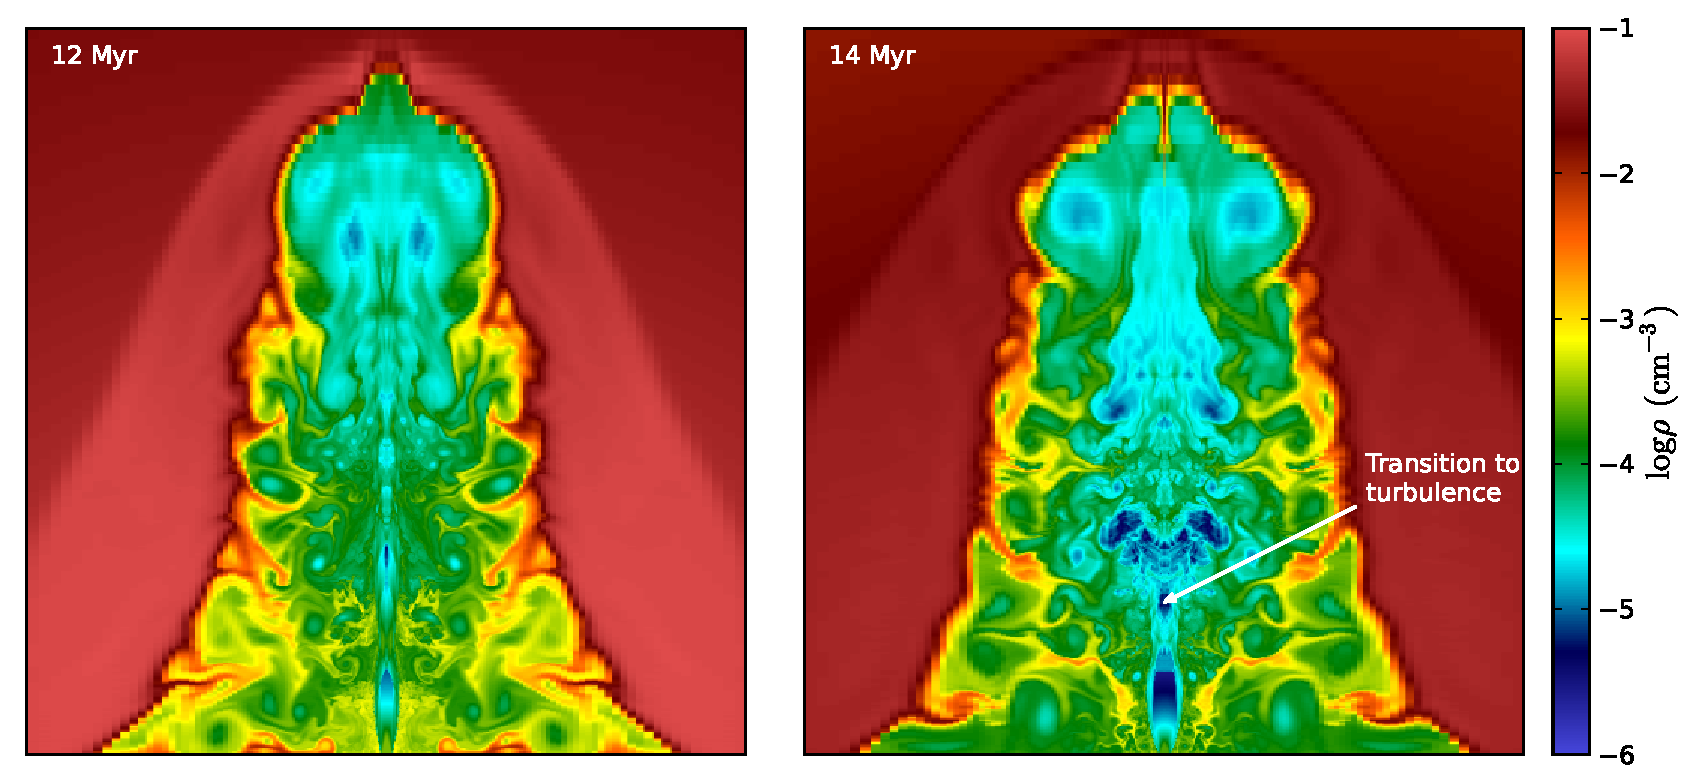
\includegraphics[width=\linewidth]{pls.eps}
\caption{Logarithmic density maps for simulations with a less over-pressured jet (run Cvb) and a sfignificantly over-pressured jet (run Cva). The comparison shows how the lobe structure differs for conical reconfinement shocks (left) and Mach disks (right), the latter being more effective in decelerating the jet and causing a turbulent transition. The dimension in each panel are ($50\,\mathrm{kpc}\times50\,\mathrm{kpc}$).}
\label{shock_comparison}
\end{figure*}
%It is possible that the northern jet undergoes a transition to turbulence associated with a Mach disk, while the southern jet transitions more gradually to turbulence via deceleration through conical reconfinement shocks


\begin{figure}
\centering
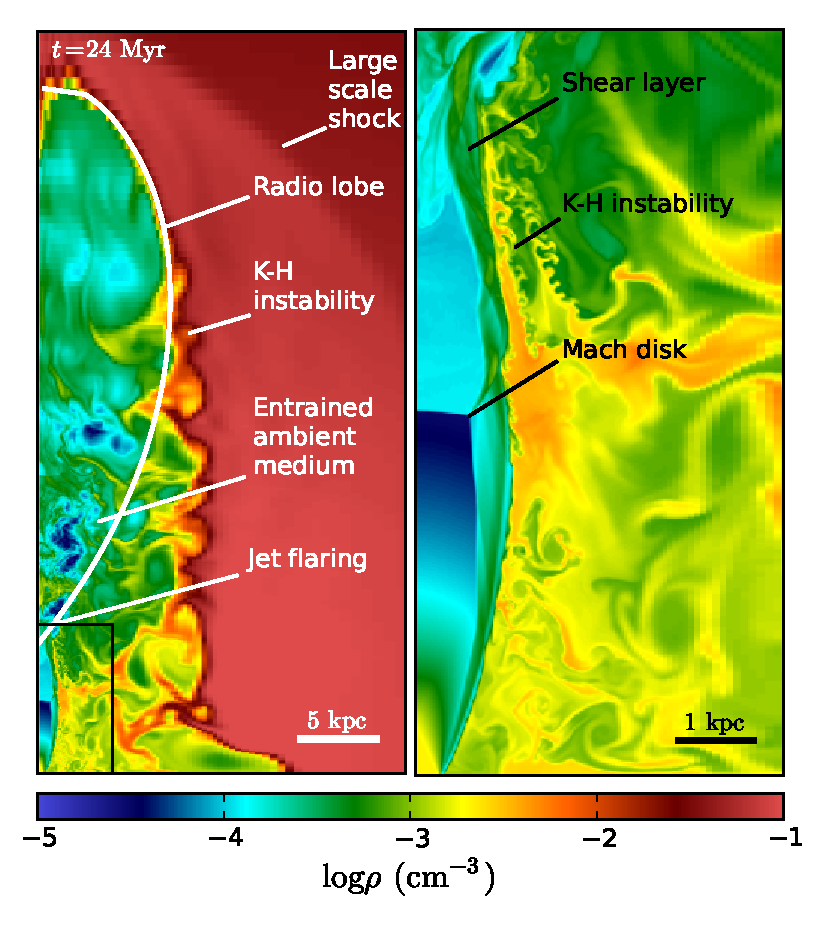
\includegraphics[width=\linewidth]{pbm.eps}
\caption{Logarithmic density map snapshot for run Av at $24\,\mathrm{Myr}$, labelling the main features of the jet-ICM interaction seen in simulations that exhibit a Mach disk. The right panel is a magnification of the central region marked with a box in the left panel.}
\label{f:morph}
\end{figure}


Fig. \ref{shock_comparison} shows two different lobe structures, one fed by a jet displaying shock diamonds (left panel), the other fed by a jet containing a Mach disk (right panel). These are snapshots from runs Cvb and Cva, respectively. Here two completely different types of jet and lobe morphology are seen. For the case of a less over-pressured jet ($p_{\rm{jet}}/p_{\rm{a}}=5$, run Cvb) the jet reconfinement proceeds through a series of shock diamonds. The jet remains coherent well inside the lobe and a number of conical shocks mediate a gradual transition to turbulence. In the other case of a jet over-pressured significantly by a factor of 10 (run Cva, right panel), the reconfinement results in a Mach disk. Although the association of a Mach disk with the northern jet bright knot consistently explain the morphology of the northern jet, I do not completely disregard the possibility of the association of a conical shock with the bright knot. Hence, in the following I determine the location of the first shock, either conical or normal, when I examine the dependence of the location of the northern bright knot on jet velocity.

%We see a violent transition to turbulence associated with the  disruptive Mach disk. These morphological features suggest that i) the northern jet of Hydra A is associated with a Mach disk, which causes both the bright knot and the subsequent rapid turbulent transition, and ii) the southern Hydra A jet can be explained by a more coherent jet associated with conical shocks which mediate a less violent turbulent transition. The association of a Mach disk and conical shocks with the northern and southern jet respectively, is also supported by the presence of the bright knot in the northern side and lack of a corresponding feature in the southern side. The increase in particle density and magnetic field associated with  oblique conical shocks are not as strong as the increase associated with a mach disk. The bright knot inside the southern lobe may be associated with a shock produced as the curved supersonic jet hits the cavity wall and abruptly changes direction. 


Fig. \ref{f:morph} shows the density image of the simulation Av at 24 Myr. I select this particular model as the fiducial model for the jets of Hydra A with a jet kinetic power of $P_\mathrm{jet}=1\times10^{45}\,\mathrm{erg}\,\mathrm{s}^{-1}$, because it clearly reproduces the transition of the jet to a turbulent plume at $\sim10$ kpc as indicated by the observations of the Hydra A northern jet. While this simulation snapshot represents the earliest phase of the development of the Hydra A plumes, I will assume that it is indicative of the dynamics in the inner $\sim10$ kpc of the jet during the subsequent evolution of the source. 

In this simulation, a Mach disk appears at $\sim6$ kpc from the jet inlet. I associate this Mach disk with the bright knot in the Hydra A northern jet. The shock-accelerated electrons and the compression of the magnetic field increase the synchrotron emission immediately behind the Mach disk and produce a bright radio knot. Downstream of the Mach disk, the jet flow is further decelerated and  becomes turbulent. The deceleration distance behind the Mach disk is $\sim 4$ kpc, in agreement with the observed distance between the bright knot at $\sim6$ kpc and the beginning of the turbulent plume at a distance of $\sim10$ kpc from the radio core. 

%The position of the Mach disk at $\sim6$ kpc in the Hydra A northern jet is consistent with the theoretical prediction of the position of the first reconfinement shock by \citet{stawarz06}. In their study of knot HST-1 in the M 87 jet they use the relativistic Rankine-Hugoniot shock jump condition to estimate the position of the first reconfinement shock. They assume that the jet is initially advancing freely and begins to reconfine at a location $r_1$, at which point it is in pressure equilibrium with the atmosphere ($p_1/p_{\rm{a}}=1$, where $p_1$ is the jet pressure at $r_1$ and $p_{\rm a}$ is the ambient pressure). In the case of Hydra A jets I estimate the starting point of the reconfinement $r_1$ by using the pressure ratio of the jet to the atmosphere at the jet inlet of the fiducial model Av ($p_{\rm{in}}/p_{\rm{a}}=10$, where $p_{\rm{in}}$ is the jet pressure at the inlet), and the jet inlet in the simulations is at a distance $r_{\rm{in}}\approx1\ \rm{arcsec}\approx1.1$ kpc from the centre of the galaxy.
%\begin{equation}
%\frac{p_1}{p_\mathrm{in}} = \frac{p_1}{p_\mathrm{a}}\frac{p_\mathrm{a}}{p_\mathrm{in}}= 1 \times \frac{1}{10} = \left(\frac{r_1}{r_\mathrm{in}}\right)^{-2\gamma}\:.
%\label{reconfinement}
%\end{equation} 
%
%We obtain $r_1=2.2$ and 2.6 kpc for a non-relativistic particle dominated jet ($\gamma=5/3$ and $\beta_2/\beta_1=1/4$) and a relativistic particle dominated jet ($\gamma=4/3$ and $\beta_2/\beta_1=1/7$) respectively. 
%
%For a jet plasma with polytropic index $\gamma$, an ambient pressure profile $p_{\rm{a}}\propto r^{-\delta}$ (where $\delta$ is the slope of the pressure profile), pre-shock velocity $\beta_1$ and post-shock velocity $\beta_2$ the analytical model for the position of the first reconfinement shock, $r_{\rm{c}}$ provided by \citet{stawarz06} is
%\begin{equation}
%r_c = r_1\left[ \frac{(2-\delta)^2(1-\beta_2/\beta_1)\gamma}{(\gamma-1)^2}\right]^{1/(2-\delta)}\:.
%\label{stawarz_reconfinement}
%\end{equation}
%
%From the atmosphere pressure profile derived in \S~\ref{s:cluster}, I estimate that $\delta=0.15$ at $\sim 6$ kpc. Solving equation~(\ref{stawarz_reconfinement}) I obtain $r_{\rm{c}}\approx7.5$ kpc for non-relativistic particle dominated jet and $r_{\rm{c}}\approx 18 \, \rm kpc$ for relativistic particle dominated jet. The position of the first reconfinement shock at $\sim 7.5 \, \rm kpc$ for the non-relativistic particle dominated jet is reasonably consistent with the result of the fiducial model Av, a Mach disk at $\sim 5 \, \rm kpc$ from the jet inlet i.e, at $\sim 6 \, \rm kpc$ from the galaxy centre. 
%
%This result reinforces the likelihood of higher values of $k$, say $k \sim 10$, as found in \S~\ref{s:p_res} and the likelihood that the jet is dominated by non-relativistic particles.

Other standard features of  simulation Av include a large-scale bow-shock advancing through the ICM, and an entrainment layer which develops between the contact discontinuity separating the shocked ICM and the shocked jet plasma. This develops as a result of the Kelvin-Helmholtz instability. 





%%%%%%%%%%%%%%%%%%%%%%%%%%%%%%%%%%%%%%%
%
%					Parameter-space Study 
%
%%%%%%%%%%%%%%%%%%%%%%%%%%%%%%%%%%%%%%%


\begin{figure*}
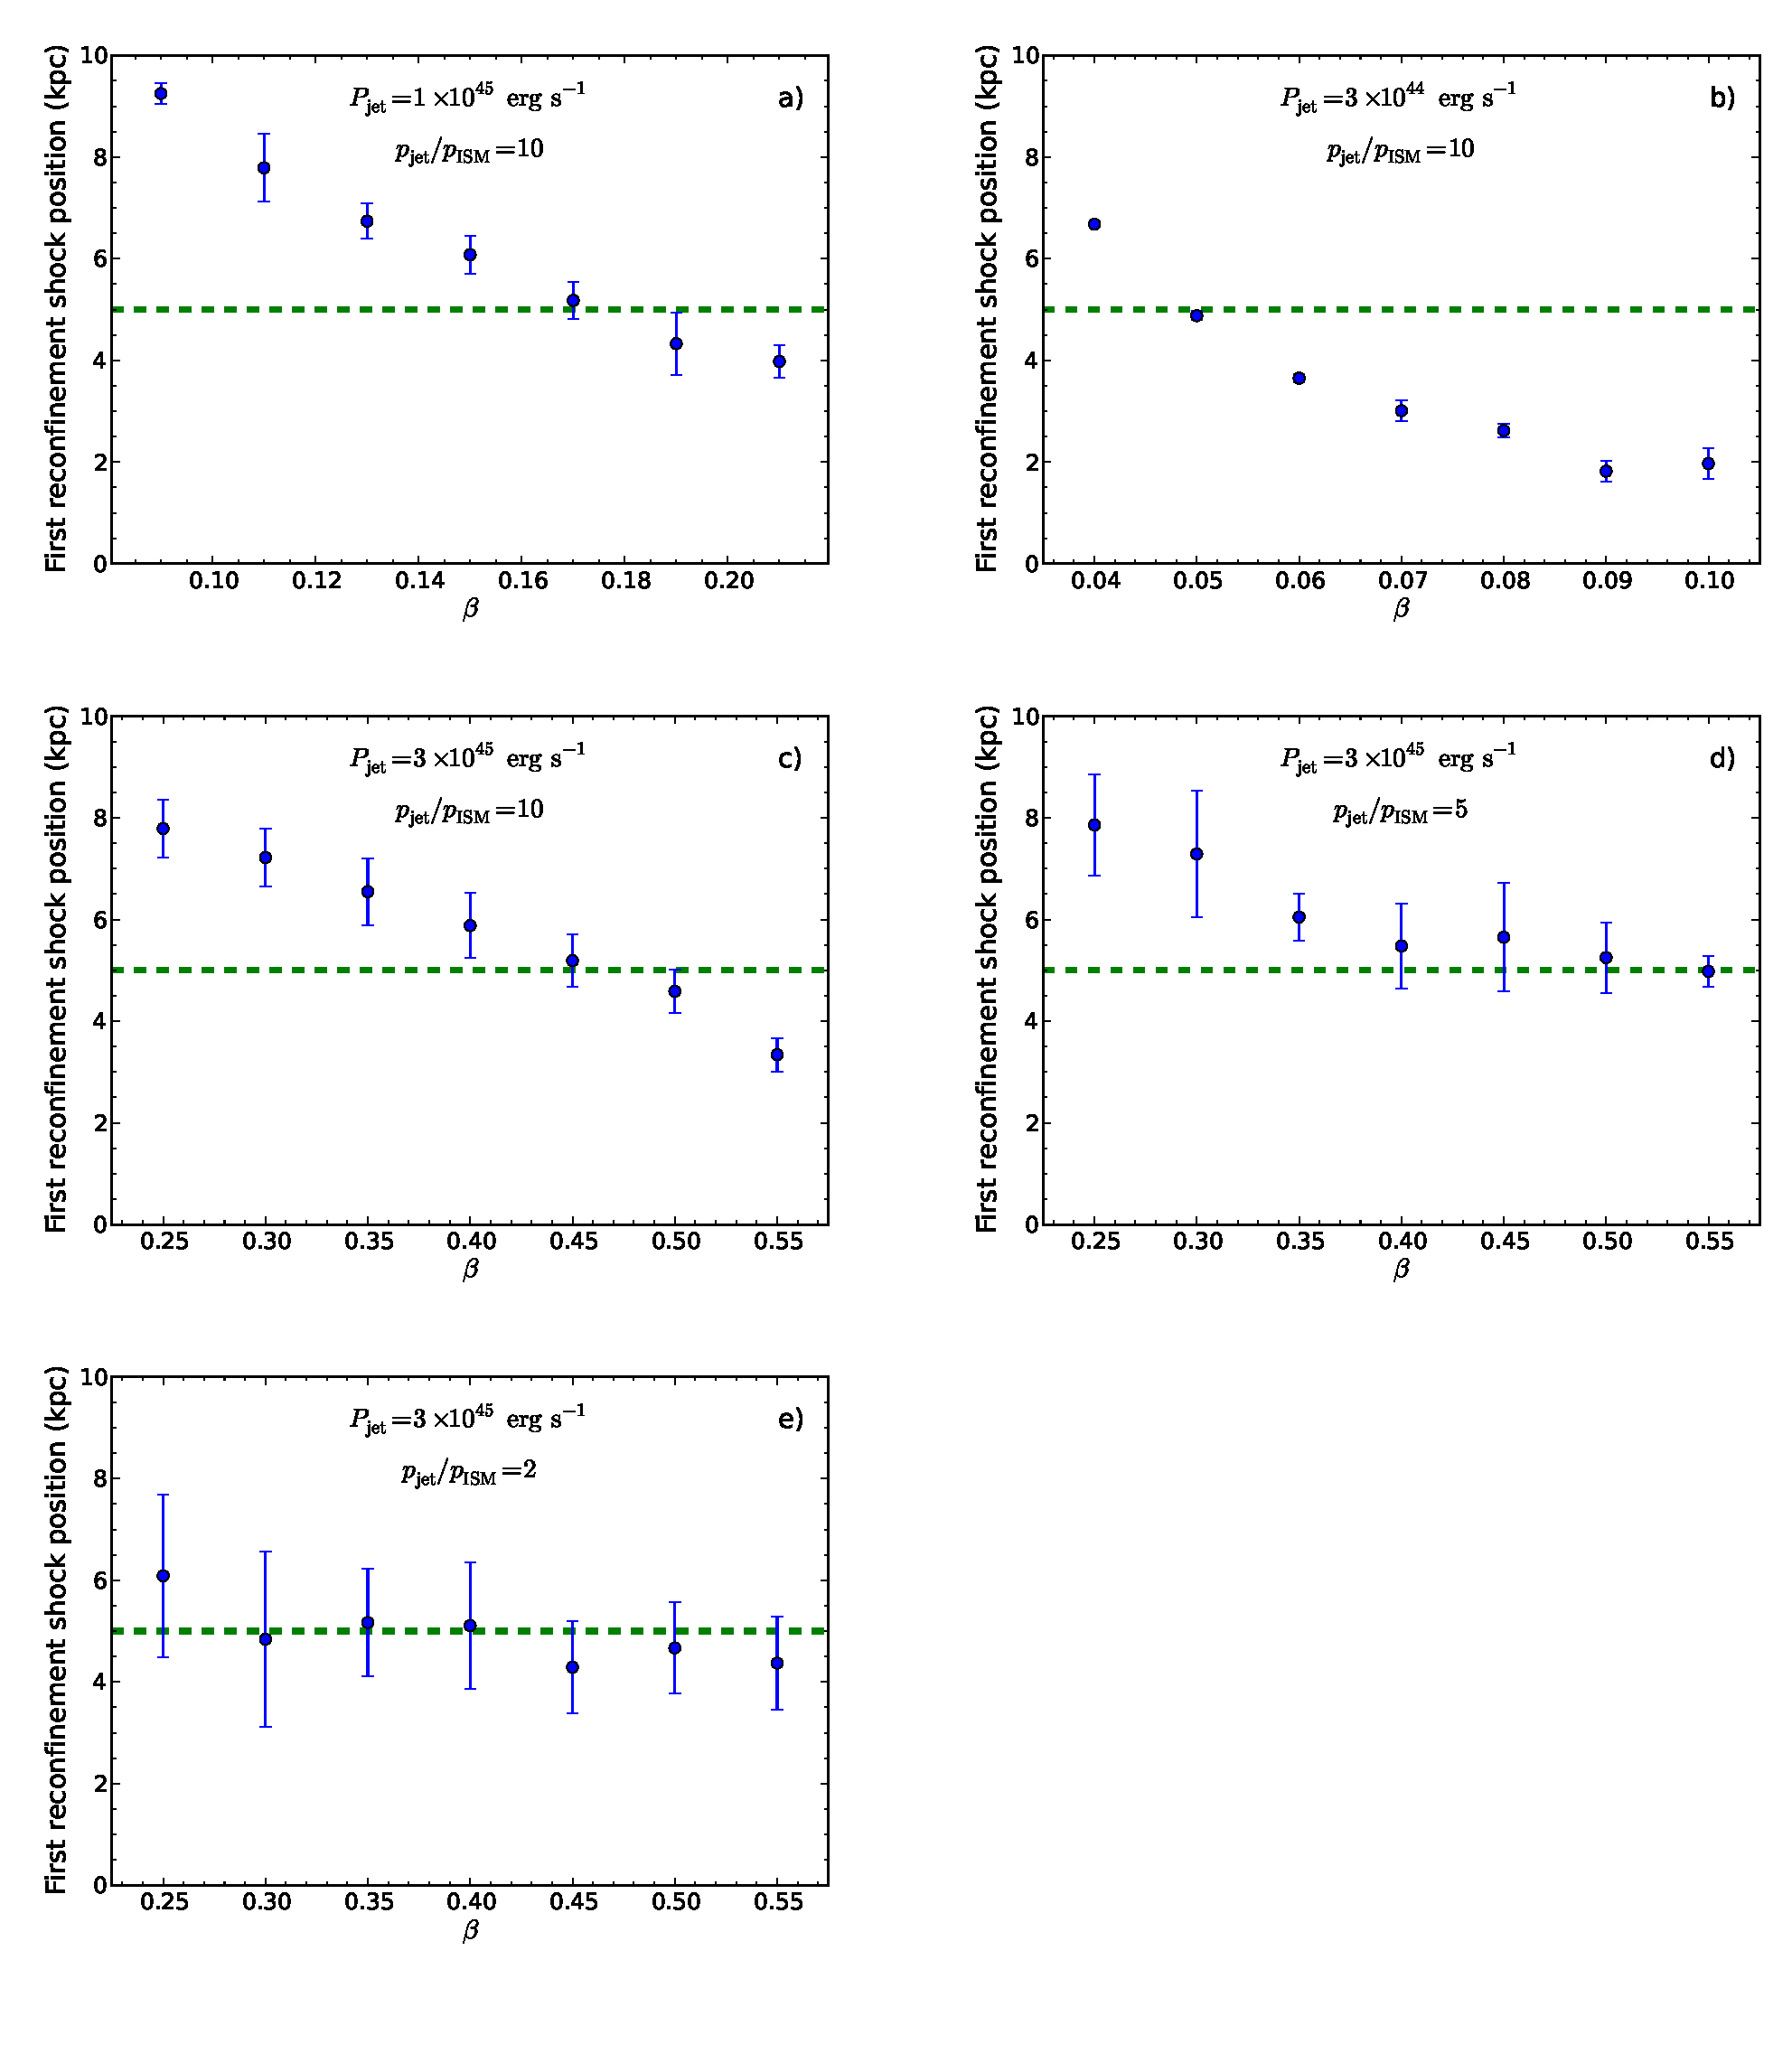
\includegraphics[width=\textwidth]{pps.eps}
\caption{Position of the first  reconfinement shock (Mach disk for significantly over-pressured jets $p_{\rm{jet}}/p_{\rm{a}}=10$ in panel a), b), and c) or the first conical shock for a relatively less over-pressured jet $p_{\rm{jet}}/p_{\rm{a}} = 5$ and 2 in panel d) and e)) as a function of $\beta$, the jet velocity in units of the light speed, measured for three sets of simulations. Each point represents the average of 25 measurements of the position of the Mach disk or first conical shock, which fluctuates with time about a mean value. The error bars represent the standard deviation of the measurements. The dashed green line at $5 \, \rm kpc$ (the first shock is assumed at $6 \, \rm kpc$ and the jet inlet in the simulation is at a distance $\sim 1 \, \rm kpc$ from the galaxy centre) in each panel represents the location of the observed southern edge of the bright knot, which I assume to be either a Mach disk or a conical shock. Measurements are for: a) parameter set A; b) parameter set B, c) parameter set Ca, d) parameter set Cb and e) parameter set Cc. These five relationships along with the assumed location of the Mach disk or the first conical shock in the northern jet at $\sim6$ kpc from the radio core lead to different acceptable jet velocities $0.17\,c$, $0.05\,c$, $0.45\,c$, $0.4-0.55\,c$ and $0.25 - 0.55\,c$ with three different jet kinetic powers $1\times10^{45}$ erg s$^-1$ (our fiducial value), as well as lower and higher values of $3\times10^{44}$ erg s$^-1$, and $3\times10^{45}$ erg s$^-1$.}
\label{mach_position}
\end{figure*}


\subsection{Results of parameter-space study}
\begin{figure}
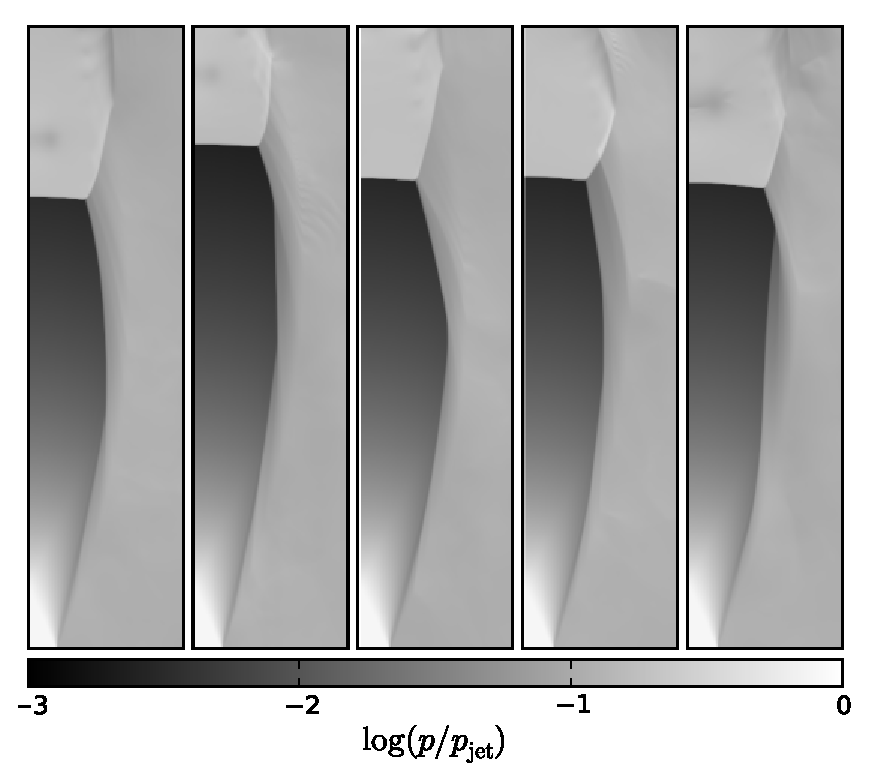
\includegraphics[width=\linewidth]{pml.eps}
\caption{Five snapshots of the logarithmic pressure maps of run Av. The sequence shows the Mach disk moving with time about a mean position. The dimensions of each panel are $2\,\mathrm{kpc}\times8\,\mathrm{kpc}$. The time interval between each snapshots is $100\,\mathrm{kyr}$.}
\label{pressure_evolution}
\end{figure}

The main aim of the parameter space study is to determine the relationship between the position of the first jet shock and jet parameters, in particular, the jet velocity and the jet power. Adopting a shock location at a deprojected distance of $\sim6\,\mathrm{kpc}$ from the core, as inferred from the radio image of Fig.~\ref{taylor} and the assumed inclination angle of
$\theta=42^\circ$ \citep{taylor90}, I use these relationships to constrain the jet velocity of the northern Hydra A jet.

An incentive for this approach comes from the (non-relativistic) expression for the natural wavelength of a supersonic jet, $\Lambda$, with diameter, $D$, and Mach number, $M$, $\Lambda/D = 1.3\sqrt{M^2 - 1}$ \citep{birkhoff57a}.
%\begin{equation}
%\lambda/D = 1.3\sqrt{M^2 - 1}
%\label{mach_position_jet_velocity}
%\end{equation}
This relationship indicates that the spacing of jet shocks should be a function of the Mach number and hence of the velocity of the jet (given that other parameters are constrained by the jet power). I, therefore, vary the jet velocity and at the same time vary the density parameter $\chi$ to maintain a constant jet kinetic power, noting the location of the first jet shock (if one exists) for each run.

In each simulation the positions of shock structures in the jet vary with time. They oscillate about a mean position. For each run, I have therefore measured the position of the jet shock at 25 snapshots with 100 kyr time difference between each two adjacent snapshot. The points in Fig.~\ref{mach_position} show the mean position of the jet shock, and the extent of the oscillation is indicated by the by error bars which represent the standard deviation of the measurements. 

The variations in the shock positions occur because the pressure field in the backflow adjacent to the jet changes continuously as a result of the turbulence in the cocoon. An example of this is shown in Fig. \ref{pressure_evolution} which shows the position of a Mach disk at five different time steps.

Fig. \ref{mach_position} shows the dependence of the distance of the first jet shock from the jet base upon the jet velocity for three different values of the jet kinetic powers: $P_{\rm{jet}}=1\times10^{45} \rm \> erg \> s^{-1}$ (the fiducial value, see \S~\ref{jet_kinetic_power}), $P_{\rm{jet}}=3\times10^{44} \rm \> erg \> s^{-1}$ and $P_{\rm{jet}}=3\times10^{45} \rm \> erg \> s^{-1}$. These are results from the runs in Table~\ref{simulation_parameters} set A, set B, set Ca, set Cb, and Cc respectively. In panels (a), (b) and (c) the first shock is a Mach disk; in panel (d) and (e) the first shock is a conical shock.
Since the jet inlet in the simulation is at a distance $1 \, \rm kpc$ from the centre of the galaxy I locate the first shock at $5 \, \rm kpc$ in each panel to determine the jet velocities. The inferred jet velocities for each result of Fig.~\ref{mach_position} is summarised in Table~\ref{inferred_jet_velocities}.

%For future work I adopt a fiducial value for the Hydra A jet velocity of $0.17c$ and I select Av as the fiducial model for the following reasons. 

\section{Summary and discussion}
Here I summarise the results of the axisymmetric models based on the assumption that the only bright knot, apparent in Fig.~3 of \citet{taylor90}, of the inner 10~kpc Hydra A northern jet, is a consequence of a Mach disk at approximately 6~kpc. 

\begin{enumerate}
\item Among the models with the fiducial jet kinetic power $1\times10^{45}$ erg s$^{-1}$ (set A), the best fit model for Hydra A northern jet (which provide a Mach disk at approximately 6~kpc from the core) is Av. The jet velocity of the best fit model is 0.17~$c$. Using a jet-to-counterjet brightness ratio $R=1.9$ \citep{taylor96}, and an inclination of the source to the line of sight of $\theta = 42^\circ$ \citep{taylor93}, in the formula of Doppler beaming, $R={((1+\beta \cos\theta)/(1-\beta \cos\theta)})^{2-\alpha}$, I estimate a jet velocity 0.17~c. 

Therefore two completely different approaches, one based on the interaction of the jet and the atmosphere and the other based on relativistic Doppler beaming, give the same estimate for the jet velocity of Hydra A jets. However, later, using the 6~cm VLA data of Hydra A I estimate a higher jet-to-counterjet brightness ratio $R = 7$. Attributing this ratio to Doppler beaming I obtain a moderately relativistic jet velocity $\approx 0.5~c$. 

A mild relativistic jet velocity for Hydra A $\approx 0.17~c$ is also inconsistent with the theoretical estimate of jet velocity for FR I radio jets $\approx 0.8~c$ provided by \citep{laing14}.

%For the relativistic beaming estimate, I adopt a jet-to-counterjet brightness ratio $R = 1.9$ and an inclination of the source to the line of sight of $\theta = 42^\circ$ \citep{taylor96,taylor93}. This gives an estimate $\beta\approx0.17$. 

\item In the best fit model (run Av), the density ratio between the jet and the ambient medium is $\eta \approx 10^{-2}$. This density ratio is relatively higher than the typical assumption light AGN jets $\eta \approx 10^{-4}$. This relatively heavy jet can be attributed to the entrainment of the pc~scale jets with a heavy gas (\citet{dwarakanath95} detected HI gas near the core of Hydra A galaxy)near the core.

\item In model Av the internal Faraday rotation $\Psi_{20 \rm cm} = 1.42$ is also high, which is inconsistent with the observed polarisation of the jet \citep{taylor93}. Three possible explanation for this uncomfortably high value of $\Psi_{20 \rm cm}$ are: i) Equipartition between the magnetic field energy in the radio plasma and the particle energy does not obtain. The magnetic field may be less than the equipartition value, which would imply lower internal Faraday rotation; ii) A preferentially perpendicular orientation of the magnetic field with respect to the line of sight, e.g. due to a toroidal magnetic field, will give smaller values of the rotation measure. c) For random magnetic field distributions in the radio plasma, the rotation measure is decreased by a factor of $N^{1/2}$, where $N$ is the number of magnetic field reversals across the jet. 

\item If lower jet kinetic powers are assumed, the best values for the jet velocity require values of the density parameter $\chi$ that are uncomfortably large, e.g., in the case in which $P_\mathrm{jet}=3\times10^{44}\,\mathrm{erg}\,\mathrm{s}^{-1}$, $\beta=0.04$ and $\chi=3143$ (run Bi) give the best fit for the location of the jet shock. In this case the internal Faraday rotation at 20~cm is 17.76~radians, clearly inconsistent with the polarisation of the jets.

\item The scenario of higher jet kinetic power and a comparatively less over-pressured jet suggest (runs Civb, Cvb, Cvib and Cviib) a range of jet velocity from $\sim0.45$ c to $\sim0.55$ c. In the case of higher jet kinetic power and a nearly pressure equilibrium jet (runs Cic to Cviic) a mildly decreasing trend of the first conical shock position with increasing jet velocity indicates an wide range of possible jet velocities from $\sim0.25$ c to $\sim0.55$ c. These two cases involve conical shocks so that the jet remains supersonic after the first shock. 

%Large value of the jet density parameter $\chi = 116$ in this model is consistent with the inferred value of $k \sim 10$ for the Hydra A radio lobes.  
%\item 

%The only parameter with unusual values in model Av is the internal Faraday rotation $\Psi_{20 \rm cm} = 1.42$, which is inconsistent with the observed polarisation of the jet \citep{taylor93}. Three possible explanation for this uncomfortably high value of $\Psi_{20 \rm cm}$ are: i) Equipartition between the magnetic field energy in the radio plasma and the particle energy does not obtain. The magnetic field may be less than the equipartition value, which would imply lower internal Faraday rotation; ii) A preferentially perpendicular orientation of the magnetic field with respect to the line of sight, e.g. due to a toroidal magnetic field, will give smaller values of the rotation measure. c) For random magnetic field distributions in the radio plasma, the rotation measure is decreased by a factor of $N^{1/2}$, where $N$ is the number of magnetic field reversals across the jet. 
%
%
%\item Higher jet kinetic powers and a significantly over-pressured jet lead to a higher estimate for the jet velocity, e.g., for $P_\mathrm{jet}=3\times10^{45}$ erg s$^{-1}$, the estimated jet velocity is $\beta \approx 0.45$ (run Cva), which implies a brightness ratio between the northern and southern jets due to relativistic beaming $\approx 5$, a factor of 2.5 larger than that seen in the data \citep{taylor96}. 
%Notwithstanding the inconsistency with relativistic beaming estimates, these
%models merit further investigation in three dimensions because of the observation of possible shock structures inside the northern lobe, indicative of supersonic flow there. 
\end{enumerate}

As I stated in the beginning of the chapter, the results presented here are based on the study of the contour image of the northern jet presented in \citep{taylor90}. A careful study of the original data (which was used to produce Fig.3 of \citet{taylor90}) shows that a fainter knot is also apparent near the core (see Fig.~\ref{northern}). Therefore, in the following chapter I revised my study of the Hydra A northern jet with a further improvement of the axisymmetric model. 

Although the models presented here are inappropriate to the Hydra A northern jet and provide unusual values for the jet velocity, the density ratio of the jet and the ambient medium and the internal Faraday rotation, they shed some light on the physics of the jet-ICM interaction. For example, 

\begin{enumerate}
\item Formation of different reconfinement shocks, diamond shocks or normal shocks, depending on the pressure ratio between the jet and the ambient medium (see Fig.~\ref{pressure_comparison}). 
\item Formation of two different jet-lobe morphologies: one is a lobe fed by a jet with biconical shocks and the other is a lobe fed by a jet with a disruptive Mach disk (see \S~\ref{morphological_structure} and Fig.~\ref{shock_comparison})
\item A correlation between the jet velocity and the location of the inner jet knot. This correlation can be easily demonstrated by the relationship between the jet kinetic power $P_{\rm jet}$ and Mach number $M_{\rm}$ for a non-relativistic flow provided by \citet{sutherland07}:
\begin{equation}
P_{\rm jet} = \frac{\gamma}{\gamma - 1} p_{\rm jet} v_{\rm jet}A_{\rm jet} \left ( 1 + \frac{\gamma -1 }{2} M_{\rm}^2 \right )
\label{e:nrP}
\end{equation}
and the relationship between the shock spacing and the Mach number of the jet (equation \ref{e:birkhoff}):
\begin{equation}
\Lambda/D = 1.3\sqrt{M^2 - 1} \nonumber
\end{equation}
According to the later equation, for a lower shock spacing we require lower Mach number. Then the former equation implies that, for a fixed jet kinetic power, jet pressure and jet inlet radius, lowering the Mach number results an increase in the jet velocity. Hence there is an inverse relationship between the shock spacing and the jet velocity. This relationship suggests that the appearance of a bright knot near the core may be a remedy of the unusual low velocity for Hydra A jets. 

In the following chapter, based on two knots in the inner 10~kpc of Hydra A northern jet, I estimate a jet velocity $\approx 0.8~c$, which is theoretically reasonable for a FRI source \citep{laing14}. 

\item The Mach number of the jet is related to the jet velocity $v_{\rm jet}$, the jet pressure $p_{\rm jet}$ and the jet density $\rho_{\rm jet}$:
\begin{equation}
M = v_{\rm jet} \rho_{\rm jet}/ \gamma p_{\rm jet}.
\end{equation} 
According to equation~\ref{e:nrP} a fixed jet kinetic power, jet pressure and jet inlet radius, increase in the jet velocity results a decrease in the jet density and hence a decrease in the Faraday rotation of the source. Therefore, as above, the bright knot near the core will provide lower values of jet density and Faraday rotation. In the next chapter, modelling the Hydra A jet knot with two bright knots, I obtain a density ratio between the jet and the ambient medium $\eta \approx 10^{-4}$, which is a typical value of an AGN jet, and a Faraday rotation $\Phi \approx 10^{-2}$, which is comfortably less than unity and consistent with the observed polarisation of the jet \citep{taylor93}.
\end{enumerate}


 


%%%%%%%%%%%%%%%%%%%%%%%%%%%%%%%%%%%%%%%%%%%%%%%%%%%%%%%%%%%%%%%%%%%%%%%%
% 
%												Discussion and Summary
%
%%%%%%%%%%%%%%%%%%%%%%%%%%%%%%%%%%%%%%%%%%%%%%%%%%%%%%%%%%%%%%%%%%%%%%%%

%\section{Summary and Discussion} \label{discussion}
%
%
%The key features of the radio jets of Hydra A, which I seek to explain in this paper are the bright knot in the northern jet at $\sim6$ kpc from the core and the turbulent transition of both northern and southern jets to plume like structures at $\sim10$ kpc as evident in the radio image (see Fig.~\ref{taylor}). To this end, I have performed a series of two dimensional axisymmetric relativistic hydrodynamic simulations of the dynamical interaction of the Hydra A jets with their environment. 
%
%%% aln %%gvb
%To ensure that I use reasonable values for the jet parameters in the simulations, I have estimated the powers associated with the inner X-ray cavities of Hydra~A corresponding to the inner radio lobes utilising the 4.6~GHz radio data \citep{taylor90} and have compared them with the estimates of \citet{wise07} for the same cavities based on the X-ray data. I obtain a power of each inner cavity $\sim 10^{44} \> \rm ergs \> s^{-1}$ consistent with their estimate $\sim 2 \times 10^{44} \> \rm ergs \> s^{-1}$ within a factor of 2. Hence, I adopt their estimate of the total jet power $\sim 10^{45} \> \rm ergs \> s^{-1}$ as the fiducial value for the numerical simulation. To obtain the X-ray atmosphere profiles surrounding the Hydra A radio source within 10 kpc of the core, I have fitted and extrapolated the X-ray data from \citet{david01} towards the centre of the galaxy.
%
% 
%On the basis of the minimum pressure estimates I conclude that the parameter $k \sim 10$. High values of this parameter are supported by other recent studies: \citet{birzan08} estimated $k$ for a group of radio galaxies assuming that the radio lobes are in pressure equilibrium with the ambient medium. Their estimates include the Hydra A radio lobes at 1.4 GHz for which they obtained a value of $k \approx 13$. \citet{hardcastle10} studied the inverse-Compton X-ray emission from the outer Hydra A radio lobes and obtained values of $k \sim 17$ and 23 for minimum Lorentz factor cut-offs of $\gamma_1=1$ and 10 respectively.  
%
%Our simulation results support the idea that a Mach disk is responsible for the bright knot in the northern jet at a deprojected distance of $\sim 6$ kpc from the core. The abrupt turbulent transition of the northern jet would then be caused by the rapid deceleration of the jet following the Mach disk. In contrast, the gradual transition of the southern jet to a turbulent plume could be mediated by less disruptive, conical reconfinement shocks. However, as I have noted, this interpretation needs to be confirmed by further three dimensional simulations.
%
%Simulation Av, for which $P_{\rm{jet}}=1\times10^{45} \> \rm erg \> s^{-1}$, is the fiducial model for the inner 
%$\sim 10$ kpc radio structure of Hydra A. As expected of a jet over-pressured with respect to its environment by a factor of 10, the jet in run Av produces a Mach disc at the first reconfinement shock. The Mach disk remains quasi-stationary at $\sim 5$ kpc from the base of the jet over at least $24$ Myr.
%The jet flow in run Av is violently disrupted at the Mach disk, following which it decelerates rapidly toward a transition to turbulence at $\sim10$ kpc from the core. This matches with the observed location of the beginning of the turbulent plume in the northern region of Hydra A. The jet velocity $\beta=0.17$ for run Av is implied by the relationship between Mach disk position and jet velocity obtained from the parameter space study. 
%
%Using the jet to counter-jet brightness ratio determined by \citet{taylor96} and a jet inclination angle $\theta \approx 48^\circ$ inferred by \citet{taylor93a} from the rotation measure asymmetry I estimate a jet velocity $\approx 0.17\,c$ from standard Doppler beaming theory. Thus, two completely different approaches, one based on the dynamical interaction of the jets with the atmosphere and the other based on relativistic Doppler beaming, give the same estimate for the jet velocities. 
%
%We have also used the analytical theory developed by \citep{stawarz06} to estimate the position of the reconfinement shocks of the Hydra A jets. Adopting parameters from run Av, I find a distance to the first reconfinement shock of 7.5 kpc for a non-relativistic particle dominated jet and 18 kpc for relativistic-particle dominated jets, supporting the previous conclusions that the jets are thermally dominated. This suggests that the jets have efficiently entrained material at small radii, for example, in the region of HI clouds near the core. The interactions with parsec scale HI clouds are well below the resolution of the simulations, but warrant further investigation.
%
%One concern with the fiducial model is that the value of the internal Faraday rotation $\Psi_{20} = 1.42$, is uncomfortably large,in view of the fact that the jets are polarised at 20~cm \citep{taylor93}. However, these estimates are maximal and would be lower if the magnetic field were sub-equipartition, if the angle between the magnetic field and line of sight were large or if there are a large number of field reversals. 
% 
%Our models of Hydra A and its associated environment can explain prominent jet features of the inner 50 kpc including the bright knot on the northern side and the turbulent transition on both sides. However, the Hydra A inner jets are bent in contrast to the straight structures that I have modelled so far, using an axisymmetric approximation. For the northern jet, the curvature within 10 kpc is modest, and we expect an approximation by a straight jet to be reasonable. The existence of the  bright knot within the plume region on the southern side of the radio source, is most likely related to a shock produced by the supersonic jet flow as it deflected through more than the Mach angle off the wall of the cavity produced by the radio plasma (see Fig.~\ref{taylor}). A realistic model for this knot cannot neglect the curvature of the jet, requiring three-dimensional numerical simulations.
%
%The next paper in this series will focus on modelling the curvature of both jets and the details of the transition from jets to plumes. In the third paper of this series I will present a full three-dimensional model of the the X-ray and radio emission of Hydra A.

\chapter{Jet velocity from knot locations and radial oscillations}\label{chapter5}
%\doublespacing

%\textbf{(b)} Zoom-in of the top rectangular region in a) showing the bright knots in the northern jet. Contours are at 1.5, 2.7, 3.7, 5.1, 6.3, 7.5, 8.8, 10, 21, 37, 51, 72, 90, 103, 154, 311, and 466 mJy arcsec$^{-2}$. \textbf{(c)} Zoom-in of the bottom rectangular region in a) showing the bright knots in the southern jet. Contours are at 1.5, 2.0, 2.2, 2.7, 3.7, 5.1, 5.5, 6.0, 6.3, 6.8, 7.5, 8.8, 10, 21, 37, 51,  72, 90, 103, 154, 311, and 466 mJy arcsec$^{-2}$.

When I finished my modelling of the Hydra A northern jet based on the data presented in \citet{taylor90} (where only one knot is evident within the central 10~kpc, see Fig.~\ref{taylor}) I requested Professor Gregory Taylor to provide the original 6~cm VLA data, which I could use to study the jets near the core region more carefully and to estimate the brightness ratio of the jets. Studying the original data I realised that a fainter knot is apparent at approximately 3.7~kpc from the core in the northern jet. Therefore, a revision of the parameter space study was required in order to model both of these internal jet knots inside 10~kpc. In this section, I present my study of 2D axisymmetric jet-ICM interactions focusing on the two inner jet knots in the Hydra A northern jet. Fig.~\ref{northern} shows two bright knots marked by arrows, location of the shocks marked by $\times$, and the location of the turbulent transition of the jet to a plume marked by an arrow. 
\begin{figure}
\centering
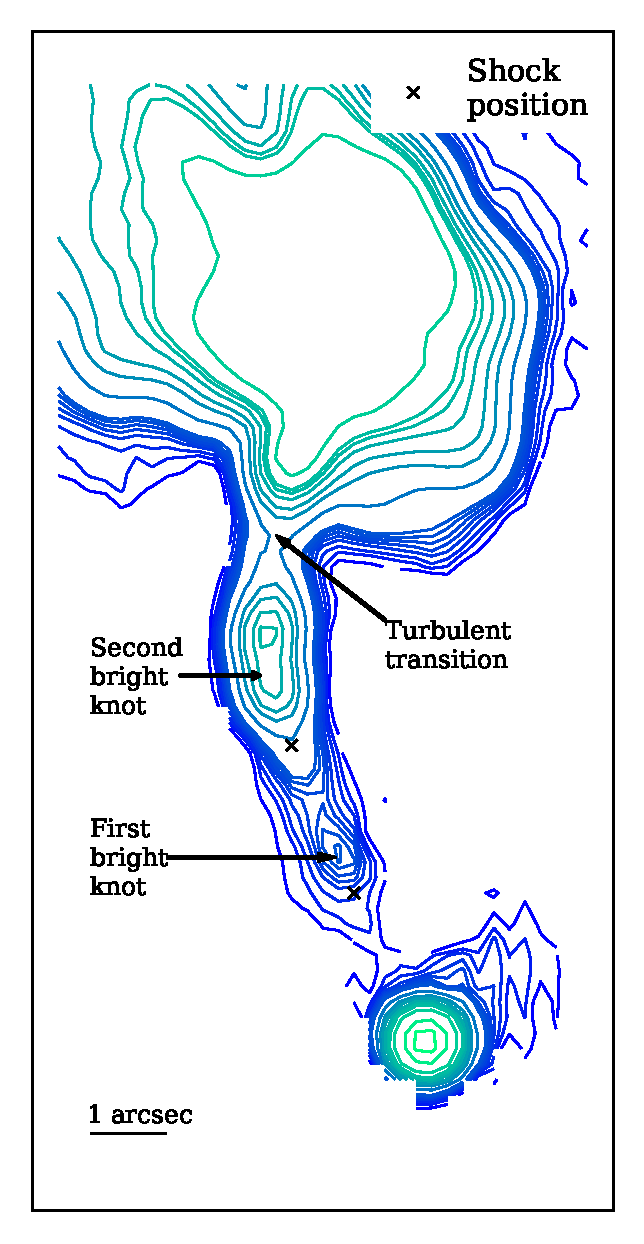
\includegraphics[width=5cm]{norhtern.eps}
\caption{Radio intensity map of the central 20~kpc region of the Hydra~A northern jet at 4.635 GHz. Contour levels are at 1.5, 2.7, 3.7, 5.1, 6.3, 7.5, 8.8, 10, 21, 37, 51, 72, 90, 103, 154, 311, and 466 mJy arcsec$^{-2}$. Two bright knots and the turbulent transition of the jet to a plume are marked by arrows. The location of the reconfinement shocks which we interpret as the cause of bright knots are marked by $\times$. }
\label{northern}
\end{figure}
%Hence, I repeated the previous parameter space study incorporating two inner knots.
Apart from incorporating two bright knots inside 10~kpc of the northern jet, I improve the axisymmetric model presented in the previous chapter with two additional features:

\paragraph{Conical opening jet:} In the numerical study of AGN jets, jets are considered to be either initially parallel \citep{sutherland07, wagner11} or initially conical \citep{komissarov98,krause12}. In the study of global effects of the jet-ambient medium interaction, for example, the mass or energy transport by the jet, it is not important whether the jet is initially parallel or conical. However, structures such as reconfinement shocks along the jet axis, are sensitive to the initial jet radius and the opening angle of the jet. Moreover, the fact that AGN jets are emitted from the black hole implies that they are initially expanding. For instance, the VLBI pc scale data \citep{taylor96} and VLA kpc scale data \citep{taylor90} of the Hydra A indicate that the jets expand from approximately 1~pc to approximately 200~pc. Therefore, for the modelling of jet structures near the core, a conical opening jet is more realistic. In the models presented in this chapter I use initially conical jet model following \citet{komissarov98}. 

\paragraph{Oscillatory nature of the jet boundary:} Oscillation of the jet boundary is a natural consequence of periodic reconfinement shocks \citep{prandtl1907, sanders83}. From the deconvolved FWHM of the jets of Hydra A \citep{taylor90}, a radial oscillation is apparent (see Fig. 6 of \citet{taylor90} and Fig.~\ref{f:radius} in this chapter). I did not consider the radial oscillation in the study presented in chapter~\ref{chapter4}. In this chapter, I consider both the knot locations and the oscillation of the jet boundary in modelling the northern jet.
%I started my study of the radio jets of Hydra A and its interaction with the cluster environment focussing the bright knot at approximately 3.7 and 7~kpc (deprojected) from the core. As explained in Chapter~\ref{introduction} and \ref{chap2} my proposal is that these two bright knots are a consequence of biconical shocks produced by the interaction of an over pressured jet with the cluster environment. 

Here I present a model of conically expanding jet entering the computational domain and interacting with the environment. I record the location of the shocks and the oscillation of the jet radius for a large number of models with different jet parameters. Both the shock locations and the oscillation of the jet boundary are used as fitting parameter to constrain the jet parameters, the jet radius $r_{\rm jet}$, the over-pressure ratio $p_{\rm jet}/p_{\rm a}$, the jet density parameter $\chi$ and the jet velocity $v_{\rm jet}$. The results are then analysed to obtain a best fit model for the Hydra A northern jet. The results of this study have been published in the journal MNRAS (Nawaz, M. A., Wagner, A. Y., Bicknell, G. V., Sutherland, R. S., and McNamara, B. R. 2014, MNRAS, 444, 1600).



%%%%%%%%%%%%%%%%%%%%%%%%%%%%%%%%%%%%%%%%%%%%%%%%%%%%%%%%%%%%%%%%%%%%%%%%
%
%												Description of Modelling
%
%%%%%%%%%%%%%%%%%%%%%%%%%%%%%%%%%%%%%%%%%%%%%%%%%%%%%%%%%%%%%%%%%%%%%%%%
\section{Jet parameters} \label{s:model}


 
\begin{figure}
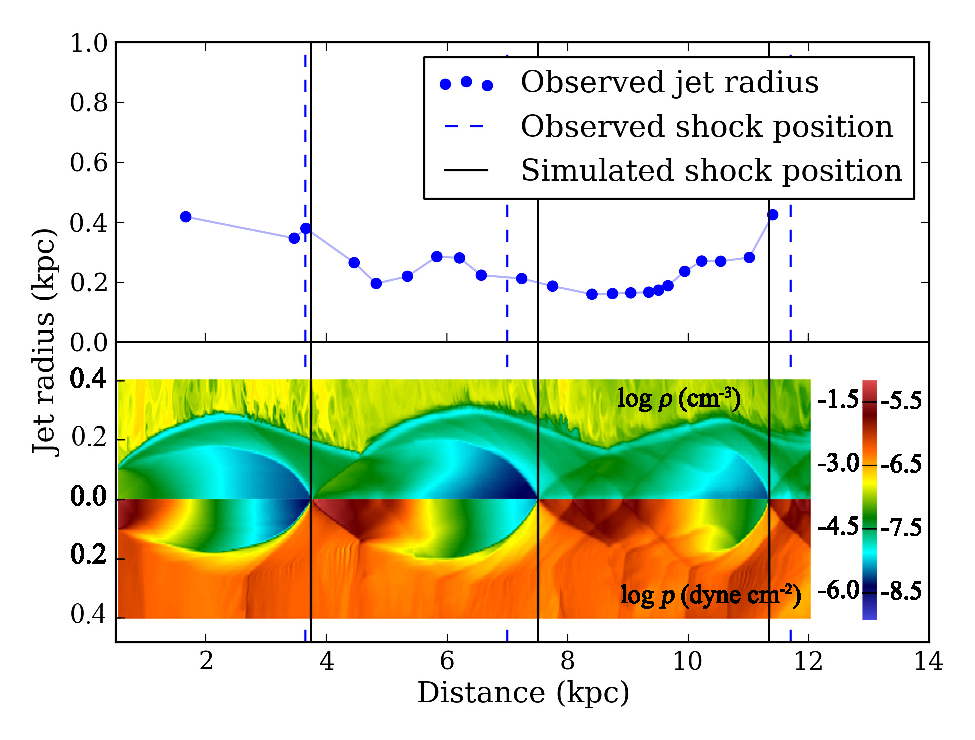
\includegraphics[width=\linewidth]{crp.eps}
\caption{Plot of the jet radius of the northern jet and the location of shocks as a function of the deprojected distance from the core. The radius is estimated from the deconvolved FWHM (see text). The vertical dashed lines represent the location of the southern edge of the first two bright knots in the northern jet, which correspond to the assumed locations of the shocks. In the bottom two panels the simulated logarithmic density and pressure slices show the periodically expanding and reconfining morphology and the shocks produced in the best-fit model for the northern jet. Both the radius plot and the images are stretched in the radial direction, emphasising the wave-like nature of the jet boundary. The vertical solid lines represent the shock positions in the simulations. The colourbar represents $\log \rho$ on the left and $\log p$ on the right.}
\label{f:radius}
\end{figure}


In this section I describe the selection of the initial jet parameters, the jet cross-sectional area $A_{\rm jet} = (\pi r_{\rm jet}^2$, where $r_{\rm jet}$ is the jet inlet radius), the jet pressure $p_{\rm jet}$, the jet density parameter $\chi = \rho_{\rm jet} c^2 / (\epsilon_{\rm jet} + p_{\rm jet})$, where $\rho_{\rm jet}$ and $\epsilon_{\rm jet}$ are the rest mass density and the energy density of the jet respectively and the jet Lorentz factor $\Gamma = (1- \beta^2)^{-1/2}$.  These parameters are assigned so as to be consistent with the expression for the jet power (equation~\ref{jet_power}).
%\begin{equation}
%P_{\rm{jet}} = \frac{\gamma}{\gamma -1} c p_{\rm{jet}}\Gamma^2\beta A_\mathrm{jet}\left(1+\frac{\Gamma -1}{\Gamma}\chi\right)\:.
%\label{jet_power}
%\end{equation} 
%\citep{sutherland07a}


\subsection{Magnetic field}\label{s:mag}	


In the simulations I neglect the magnetic field. Is this a reasonable approximation given the popular notion that jets may be collimated by the toroidal field, which develops as a result of the rotation of the flow ejected from the accretion disk \citep{blandford82a} or from the ergosphere \citep{blandford77a}? In this case one expects the magnetic and particle pressures to be comparable. Moreover, this would argue against the assumption of invoking an over-pressured jet on the parsec-scale (see below). Self-collimation by a toroidal magnetic field is an appealing mechanism for the region of jets just outside the Alfven surface. However, the fact that the jet expands by a factor of over 200 between the parsec scale and the kiloparsec scale indicates that self-collimation does not occur in this region. For example the self-similar models of \citet{li92a} and \citet{vlahakis03a} indicate that asymptotically the flow becomes cylindrical when the jet is magnetically collimated. A different model has been proposed by \citet{spruit11a}, who has argued that three-dimensional effects lead to reconnection of the magnetic field and that the loss of magnetic energy produces a pressure gradient, which is responsible for the acceleration of jets to high Lorentz factors. \citet{moll09a,moll10a} has carried out numerical simulations based on this concept, in the context of protostellar jets. There is also observational support for 
sub-equipartition magnetic fields on the sub-parsec scale in a substantial fraction of gamma ray blazars. In a recent paper \citet{zhang14a} modelled the spectral energy distributions of a number of BL~Lac objects and flat spectrum radio quasars (FSRQs) and found that they divide along the line magnetic~power = electron~power with most of the BL~Lac objects being below this dividing line (see their Fig. 13(b)). The respective powers are proportional to the energy densities of the various components (their section 4) so that the ratio of the magnetic power to electron power informs us of the ratio of the respective energy densities. Hence, the magnetic energy densities in many of the BL~Lac objects are well below the electron energy density (but with some members of the sample approaching equality). Thus there is good justification, in the first instance, for neglecting the magnetic field with the implication that the beamed counterpart of Hydra~A would be a BL~Lac object rather than a quasar. 

 
What values of the jet density parameter, $\chi$ are relevant in this context? Two main options for jet composition are generally discussed -- electron-positron or electron-proton. Let $m_e$ be the electron mass and $m_+$ the mass of the positively charged component, $m_e$ for a positron and $m_p$ for a proton. The parameter $\chi$ is then given by: 
\begin{equation}
\chi = 0.75(a-2)(a-1)^{-1} \, \frac {m_+}{m_e} \gamma_1^{-1},
\end{equation}
where $a$ and $\gamma_1$ are defined in \S~\ref{s:powr}. Note that, for an electron positron jet with $a=2.4$ and $\gamma_1 \gtrsim 10$, $\chi \ll 1$. The theory of jet production from black holes \citep{blandford77a} and X-ray observations of the lobes of both FR1 and FR2 radio galaxies \citep{croston05a,croston14} make the concept of electron-positron jets appealing. However, the issue of jet composition is by no means settled. In an electron-proton jet, low values of $\chi$ require the low energy cutoff, $\gamma_1 \gg 1$. 


\subsection{Over-pressured jets}\label{s:opj}

A key feature of the jet model is that the bright knots beginning at $\sim3.7$ and 7.0 and 11.0 kpc from the core in the northern jet and at $\sim 2.5$, 3.9, 5.4 and 6.7 kpc in the southern jet are the result of  consecutive biconical shocks following recollimation of over-pressured jets. I have identified the points where the surface brightness gradient markedly increases, as the location of the upstream side of each knot (See Fig.~\ref{northern} and Fig.~\ref{southern}). The third knot in the northern jet occurs just as the jet merges into the lobe so that I might expect the location of this knot to be affected somewhat by the jet's transition to turbulence.  

\citet{norman82} first drew attention to the production of biconical and normal shocks (Mach discs) in over-pressured astrophysical jets. An initially over-pressured jet expands laterally and its thermal pressure and ram pressure decreases with distance along the direction of propagation. When the jet pressure reaches the ambient pressure the jet begins to recollimate. The jet periodically expands and recollimates, producing a series of biconical or normal shocks along the jet axis. This phenomenon had been known to laboratory hydrodynamicists for some time and \citet{birkhoff57a} associated it with the \emph{natural wavelength} of a supersonic jet $\Lambda$ (see equation~\ref{e:birkhoff}). 

It is feasible that the Hydra A jets are initially over-pressured since the minimum energy pressure in the pc-scale northern jet, 27 pc from the central black hole \citep{taylor96} is $1.33\times10^{-7}$ and $1.26\times10^{-7} \rm \ dynes \ cm^{-2}$ for $\beta=0.2$ and 0.9 respectively. (A jet diameter of 26 pc was used in these estimates). These minimum energy pressure estimates are about a factor of 200 times higher than the central pressure $\approx 6.6\times10^{-10} \rm \ dynes \ cm^{-2}$ of the modelled interstellar medium (see \S~\ref{s:cluster}). Moreover, using these pressures underestimates the jet kinetic power at $ \approx 2.4 \times10^{44} \ \rm erg \ s^{-1}$ for $\beta =0.8$ and $\chi \sim 10^{-2}$ compared to the value $10^{45} \ \rm erg \ s^{-1}$ used in the models by a factor $\approx 4$. Therefore the value of the jet kinetic power of the models implies a jet pressure $6~\times p_{\rm min} \approx 7.0 \times 10^{-7} \rm \ dynes \ cm^{-2} $ at 27~pc. This is approximately 100 times the central atmosphere pressure. If I assume that the jet expands adiabatically, i.e., the jet pressure decreases with the jet radius according to $p_{\rm jet}\propto r_{\rm jet}^{-8/3}$, I obtain an over pressured jet $5~p_{\rm a}$ at 0.5~kpc  from the core (where I initialise the jet in the computational domain) with a jet radius 100 pc. 


Interpreting the jet as over-pressured on the parsec scale implies that from the parsec to the kiloparsec scale it is freely expanding. I also note here that, in a detailed analysis of protostellar jets \citet{cabrit07a} has concluded that those jets are initially magnetically collimated but are freely expanding at some distance ($\sim 50 \> \rm AU$) from the star. Of course, these scales are not directly commensurable with Hydra~A, but a long held view is that the physics of protostellar and AGN outflows are similar in many respects.


The proposition of the jet bright knots as biconical shocks is further reinforced by the observed wave-like nature of the northern jet boundary. Fig~\ref{f:radius} shows the radius profile (dots) of the northern jet, which I obtain by assuming the jet as a homogeneous cylinder and utilising the deconvolved FWHM of the jet \citep{taylor90} $\Phi_{\rm jet}$ together with $r_{\rm jet} = \Phi_{\rm jet}/ \sqrt{3}$. In order to illustrate the association of biconical shocks with the sinusoidal radius profile I attach the logarithmic density and pressure images (panels marked with $\log\rho$ and $\log p$ respectively) of one of the best fit models Ciii for the northern jet. In the simulated radius profile I see the jet boundary oscillates and at $\sim 0.7 \ \rm kpc$ before each radius minimum biconical shocks appear. These are clearly indicated by the large increase in pressure. The observed and simulated shock locations are marked with dashed and solid vertical lines respectively.

I construct models of the northern jet for which data on the jet FWHM are more complete. The modelling strategy for this jet is as follows. I conduct a parameter space study searching for numerical models which can successfully reproduce the correct shock locations and the radius profile of this jet. 

In the axisymmetric numerical models of the jet-ICM interaction I deal with straight jets whereas the Hydra A jets are curved. However since the curvature of the jets are modest within the central 10~kpc, I expect an approximation by a straight jet to be reasonable.

As stated above, in order to model the jets of Hydra A I require five jet parameters, the jet kinetic power $P_{\rm{jet}}$, the initial jet radius $r_{\rm{jet}}$, the initial jet pressure $p_{\rm{jet}}$, the initial jet velocity $\beta$ (in units of the speed of light), and the jet density parameter $\chi$, of which four are independent. In the previous section I established a value for the jet kinetic power $10^{45} \rm erg \ s^{-1}$. In the following I describe how I choose the other three independent jet parameters and set their values. 

The first parameter is the jet kinetic power, which is reasonably well-determined by the radio and X-ray observations. The jet radius is the second parameter; this affects the downstream scale of the oscillating jet boundary and is not known \emph{ab initio}. The third parameter is the jet pressure ratio; this affects both the amplitude of the radial oscillations and the knot spacing. The fourth parameter is the jet velocity, $\beta$. Then the parameter $\chi$ is determined using equation~\ref{chi2}.
%by solving equation~(\ref{jet_power}) for $\chi$, that is,
%\begin{equation}
%\chi = \frac{\Gamma}{\Gamma -1}\left( \frac{\gamma-1}{\gamma}\frac{P_{\rm{jet}}}{c p_{\rm{jet}} \Gamma^2\beta A_{\rm{jet}}} -1 \right)\:.
%\label{chi2}
%\end{equation}

Referring to the expression for the natural wavelength $\Lambda$ of a supersonic \emph{non-relativistic} jet in near pressure equilibrium $\Lambda/r_{\rm jet} \approx 2.6 \sqrt{M^2 - 1}$
% \begin{equation}
%\Lambda/r_{\rm jet} \approx 2.6 \sqrt{M^2 - 1}
%\label{e:birkhoff}
%\end{equation}
\citep{birkhoff57a}, I note that the selection of the velocity and density parameters is equivalent to defining the Mach number, 
\begin{equation}
M = (2+3 \chi)^{1/2} \Gamma \beta
\end{equation} 
\citep{bicknell94a}. 
%$=(2+3 \chi)^{1/2} \Gamma \beta$ \citep{bicknell94a}. 

Following \citet{komissarov98} and \citet{krause12} I model the jet as ballistic and conically expanding in the first 
0.5~kpc, which represents the base of the computational domain. \citet{komissarov98} used an identical setup in their simulations to show that an initially conical jet may be collimated by the ambient pressure. \citet{krause12} performed simulations, also with identical initial conditions to provide a theoretical basis for the FRI/FRII classification of radio sources based on the half cone angle of the initial jet cone.

To summarize, I set up my simulations with an initially over-pressured (in one case equilibrium pressure) conically expanding jet with cross-sectional radius $r_{\rm{jet}}$ and centre at $(r, z) = (0, 0.5)$ kpc, where $r$, and $z$ are the radial and height coordinate of the axisymmetric cylindrical domain.  The independent jet parameters are jet power $P_{\rm{jet}}=10^{45}\,\rm erg \, s^{-1}$, jet radius $r_{\rm{jet}}$, inlet jet pressure $p_{\rm{jet}}$, inlet jet velocity $\beta$. The remaining jet parameter $\chi$ is determined from Eqn.~\ref{chi2}
The components of the jet velocity at a points $(r, z)$ within the initial conically expanding jet cross-section are $v_r = \beta z/\sqrt{r^2 + z^2}$ and $v_z =\beta r/\sqrt{r^2 + z^2}$. 


%%%%%%%%%%%%%%%%%%%%%%%%%%%%%%%%%%%%%%%%%%%%%%%%%%%%%%%%%%%%%%%%%%%%%%%%
%
%												CODE AND SIMULATION PARAMETERS
%
%%%%%%%%%%%%%%%%%%%%%%%%%%%%%%%%%%%%%%%%%%%%%%%%%%%%%%%%%%%%%%%%%%%%%%%%
\section{Grid of models} \label{s:code}

%% TBD Fix table with new values of n_e (done)

%\begin{table*}
\begin{sidewaystable}[htbf]
\caption{Simulation parameters. In all simulations, $P_{\rm{jet}}=10^{45} \rm \ erg \ s^{-1}$.}
\centering
\begin{tabular}{l * {9}{c}}
\hline \hline
Model  & $r_{\rm{jet}}(pc)$ & $p_{\rm{jet}}/p_{\rm{a}}$ & $\beta$ & $\chi$ & $\eta$ & $\phi$ (rad cm$^{-2}$) & $\Psi_{6\rm{cm}}$ (rad) & $\Psi_{20\rm{cm}}$ (rad) \\
\hline
    %%%%%%%%%% 		set A 	%%%%%%%%%%%%%%%
%	\multicolumn{9}{c}{Set A, $r_{\rm{jet}}=0.18 \rm \ kpc$} \\ 
	\hline
	 Ai    &  180 &   2  &  0.40  &     251.19 &   5.62$\times10^{-3}$  &    4.95$\times10^{-4}$         &     1.78$\times10^{-2}$		&  1.98$\times10^{-1}$      \\	 
  	 Aii 	& 180 &  	2  &  0.70 & 	23.17 &	 5.18$\times10^{-4}$ & 	4.56$\times10^{-5}$ 	&	1.64$\times10^{-3}$		&  1.83$\times10^{-2}$	  \\
	 Aiii 	& 180 &  	2  &  0.75 & 	15.03 &	 3.37$\times10^{-4}$ &	2.97$\times10^{-5}$ 	&	1.07$\times10^{-3}$		&  1.19$\times10^{-2}$	  \\
	Aiv 	& 180 & 	2  & 	0.80 & 	9.27   &  	2.07$\times10^{-4}$  &	1.83$\times10^{-5}$		&	6.57$\times10^{-4}$ 	&  7.30$\times10^{-3}$	 \\
	Av 	& 180 & 	2  & 	0.85 & 	 5.10  & 	1.14$\times10^{-4}$ &	 1.01$\times10^{-5}$	& 	3.62$\times10^{-4}$		&  4.02$\times10^{-3}$  	 \\
	 Avi 	& 180 & 	2  &	0.90 &  	2.14   & 	4.79$\times10^{-5}$  &	 4.22$\times10^{-6}$	&  	1.52$\times10^{-4}$		&  1.69$\times10^{-3}$ 	\\
	 Avii  &  180  &  2  & 0.95  &   0.11  &   2.40$\times10^{-6}$       &    2.11$\times10^{-7}$		&	7.60$\times10^{-6}$		&   8.45$\times10^{-5}$  \\
		\hline
	  %%%%%%%%%% 		set  B	%%%%%%%%%%%%%%%
%	\multicolumn{9}{c}{Set B, $r_{\rm{jet}}=0.15 \rm \ kpc$} \\ 
        Bi    &  150  & 2  &  0.40  &   366.98  & 8.21$\times10^{-3}$  & 6.02$\times10^{-4}$ 	& 	2.17$\times10^{-2}$ 	& 	2.41$\times10^{-1}$  \\
  	 Bii 	& 150 &  2  &  0.70 &   34.90 & 7.80$\times10^{-4}$  &	5.73$\times10^{-5}$		&	2.06$\times10^{-3}$		&	2.29$\times10^{-2}$  \\
	 Biii 	& 150 &  2  &  0.75 &   23.00 & 5.14$\times10^{-4}$  &	3.78$\times10^{-5}$		&	1.36$\times10^{-3}$		&	1.51$\times10^{-2}$  \\
	Biv 	& 150 & 2  &  0.80 & 14.45   & 3.23$\times10^{-4}$   &	2.37$\times10^{-5}$		&	8.54$\times10^{-4}$ 	&  	9.49$\times10^{-3}$	 \\
	Bv 	& 150 & 2  &  0.85 &  8.28  & 1.85$\times10^{-4}$     &     1.36$\times10^{-5}$		&	4.89$\times10^{-4}$		&   	5.44$\times10^{-3}$	 \\
	Bvi 	& 150 & 2  &  0.90 & 3.87  &  8.64$\times10^{-4}$     &	6.34$\times10^{-6}$		&	2.28$\times10^{-4}$		& 	2.54$\times10^{-3}$ 	\\
	Bvii 	& 150 & 2  &  0.95  & 0.79 & 1.78$\times10^{-5}$	&    1.30$\times10^{-6}$		&      4.69$\times10^{-5}$		&      5.21$\times10^{-4}$   \\
 	Bviii    & 150 & 5 & 0.70 & 11.86  & 6.63$\times10^{-4}$      & 	4.87$\times10^{-5}$		& 	1.75$\times10^{-3}$		&      1.95$\times10^{-2}$   \\
	Bix    & 150 & 5 & 0.75 & 7.43   & 4.15$\times10^{-4}$      & 	3.05$\times10^{-5}$		&	1.10$\times10^{-3}$		&	1.22$\times10^{-2}$ \\
	Bx    & 150 & 5  & 0.80  &  4.28 & 2.39$\times10^{-4}$    &    1.76$\times10^{-5}$		&	 6.32$\times10^{-4}$	& 	7.02$\times10^{-3}$  	\\
	Bxi  & 150 & 5  &  0.85 &   2.04  &   1.14$\times10^{-4}$    &	8.39$\times10^{-6}$ 	&  	 3.02$\times10^{-4}$	&  	3.35$\times10^{-3}$ \\
        Bxii   &  150 & 5  &  0.90 &   0.48  &  2.70$\times10^{-5}$   &	1.98$\times10^{-6}$ 	&    	 7.13$\times10^{-5}$	&  	7.92$\times10^{-4}$	 \\
	\hline
	  %%%%%%%%%% 		set C 	%%%%%%%%%%%%%%%
%	\multicolumn{9}{c}{Set C, $r_{\rm{jet}}=0.10 \rm \ kpc$} \\
        Ci     &  100 & 5  & 0.40    &  329.08  & 1.84$\times10^{-2}$ &   9.00$\times10^{-4}$		&      3.24$\times10^{-2}$		&      3.60$\times10^{-1}$ \\
	Cii	& 100  & 5  & 0.70  & 31.06 & 1.74$\times10^{-3}$	  &   8.50$\times10^{-5}$		&	3.06$\times10^{-3}$		&	3.40$\times10^{-2}$ \\
	Ciii	& 100  & 5  & 0.75  & 20.41 & 1.14$\times10^{-3}$ 	  &   5.58$\times10^{-5}$	 	&      2.01$\times10^{-3}$		&	2.23$\times10^{-2}$ \\
  	Civ    & 100 &  5  & 0.80  & 12.75  &  7.83$\times10^{-4}$  &   3.49$\times10^{-5}$  	&	1.26$\times10^{-3}$ 	&  	1.40$\times10^{-2}$ 	\\
	Cv   & 100 &  5  &  0.85 &   7.24   &  4.45$\times10^{-4}$  &   1.98$\times10^{-5}$ 		&  	7.13$\times10^{-4}$		&      7.92$\times10^{-3}$  \\
	Cvi   & 100 & 5  &  0.90 &   3.30  &  2.03$\times10^{-4}$   &	9.03$\times10^{-6}$  	&  	 3.25$\times10^{-4}$	&       3.61$\times10^{-3}$	 \\
	Cvii   & 100 & 5 & 0.95  & 0.57  &  3.18$\times10^{-5}$	  &    1.56$\times10^{-6}$		&      5.61$\times10^{-5}$		&       6.33$\times10^{-4}$  \\
	Cviii  & 100 &  5  &  0.96  & 0.15  & 8.33$\times10^{-6}$	  &    4.08$\times10^{-7}$		&      1.47$\times10^{-5}$		&      1.63$\times10^{-4}$ \\
	\hline
	 Di 	& 120  & 5   &  0.50    & 96.96	  & 5.48$\times10^{-3}$	 & 	3.22$\times10^{-4}$ 	&	1.16$\times10^{-2}$		&  1.29$\times10^{-1}$	  \\
	 Dii 	& 100  & 5   &  0.50 & 144.34  & 8.07$\times10^{-3}$ &	3.95$\times10^{-4}$         &	1.42$\times10^{-2}$		&  1.58$\times10^{-1}$	  \\ 
	 Diii 	& 80    & 10   &  0.50  & 111.14  &  1.24$\times10^{-2}$    &	4.86$\times10^{-4}$		&	1.75$\times10^{-2}$ 	&  1.95$\times10^{-1}$	 \\
	 Div 	& 80    & 15   &  0.50  &  71.60 	  & 1.20$\times10^{-2}$     &	 4.70$\times10^{-4}$	& 	1.69$\times10^{-2}$		&  1.88$\times10^{-1}$  	 \\
	 Dv 	& 60    & 10   &  0.50  &  203.38  & 2.27$\times10^{-2}$     &	 6.68$\times10^{-4}$	&  	2.40$\times10^{-2}$		&  2.67$\times10^{-1}$ 	\\
	 Dvi 	& 60    & 15   &  0.50  &  133.10  & 2.23$\times10^{-2}$     &	 6.55$\times10^{-4}$	&  	2.36$\times10^{-2}$		&  2.62$\times10^{-1}$ 	\\
	 \hline
\end{tabular}
\label{t:sim_par}
\end{sidewaystable}
%\end{table*}



For my simulations I use the the publicly available PLUTO code \citep{mignone07} and produce two dimensional axisymmetric hydrodynamic models of the jet-ICM interaction in Hydra A. Since my  models involve relativistic velocities I use the relativistic hydrodynamic (RHD) module available in PLUTO. Detail description of the code and the problem initialisation are given in Chapter~\ref{chapter2}.

%The $(r, z)$ computational domain for the two dimensional axisymmetric simulations is a cylinder of radius $r=25$ kpc and height $z=50$ kpc. Using a stretched grid I define a high resolution grid within the central $10\,\mathrm{kpc}\times1\,\mathrm{kpc}$ region, giving us 10 cells across the jet inlet, and a lower resolution in the outer regions. I impose an axisymmetric boundary condition for the boundary $r=0$, and a reflective boundary condition for $z=0$.  The remaining boundaries are set to outflowing boundaries.
%
%I use the \citet{taub1948a} equation of state, a quadratic approximation to the exact Synge--J\"{u}ttner relativistic perfect gas equation of state \citep{juttner1911a,synge1957a}, which yields $\gamma\rightarrow5/3$ in the low temperature limit, and $\gamma\rightarrow4/3$ in the high temperature limit. 
%Because the radiative cooling time of the ambient gas and the synchrotron cooling time of the jet plasma are large compared to the simulation time, I do not include radiative cooling in my  simulations.
%
%The initial conditions for the ambient medium representing the hot ICM surrounding Hydra A are the hydrostatic thermodynamic profiles found in \S~\ref{s:cluster}. 

To determine the optimal values for the three initial jet parameters $r_{\rm{jet}}$, $p_{\rm{jet}}$, and $\beta$ for the Hydra A northern jet, I compare the radius profile of the jet and the locations and spacing of the reconfinement shocks in my  simulations with the observed radius profile and shock positions as indicated by the locations of the two bright knots. The thirty three sets of parameters that I have used are summarised in Table~\ref{t:sim_par}. I have not utilised every possible combination of parameters since I have restrictions on the jet radius minimum of 160 pc. I have not used models with five times over-pressured jet with jet inlet radius 180 pc and two times over-pressured jet with inlet radius 100 pc since they will produce much larger or smaller minimum in the radius profile than 160 pc. Since by experimenting models with lower jet velocities I obtain significantly large shock spacing compared to the observed shock spacing, I have not presented models with $\beta < 0.4$. A grid of models with jet $\beta = 0.5$ which exhibit larger shock spacings is presented in \S~\ref{s:b_r} 

For an additional check for the consistency of the jet parameters, some derived parameters, namely the density parameter $\chi$, the density ratio $\eta$ of the jet and the atmosphere at the jet base, the rotation measure (RM) $\phi$, and the Faraday rotation angle $\Psi$ at 6 cm ($\Psi_\mathrm{6cm}$) and 20 cm ($\Psi_\mathrm{20cm}$) are also summarised in Table \ref{t:sim_par}. Unlike models with a single knot (presented in chapter~\ref{chapter4}), all of the Faraday rotation values are comfortably less than unity and in the best models, Ciii, Civ and Cv, much less than unity.

%The rotation measure and Faraday rotation of the central jet with electron density $n_\mathrm{\mathrm e,jet}$(=$\rho_{\mathrm jet}$(1 + 2 $n_{\mathrm He}$/$n_{\mathrm H}$)/u(1 + 4$n_{\mathrm He}$/$n_{\mathrm H}$), where $u$ is an atomic mass unit), magnetic field along the line of sight $B_z$ (we use $35 \> \mu\,\mathrm{G}$, approximately the minimum energy magnetic field near the jet base), differential plasma depth $dl$, jet radius $R_{\rm{jet}}$, total plasma depth $L=2R_{\rm{jet}}$, and wavelength $\lambda$ are calculated from
%\begin{eqnarray}
%\phi &=& 8.1\int n_\mathrm{e,jet} B_z dl \quad \rm rad \, cm^{-2} \nonumber \\
%&=& 8.1\times10^{-5}\, \left(n_{e, jet}\right) \left(\frac{B_z}{\mathrm{\mu G}}\right)  \left(\frac{2R_{\rm{jet}}}{\mathrm{kpc}} \right) \rm rad \, cm^{-2}
%\end{eqnarray}
%where the units of $B_z$ and $l$ are Gauss and cm, respectively. The total Faraday rotation through the jet is given by:
%\begin{equation}
%\Psi_{\rm rad} = \phi \lambda^2 \:.
%\end{equation}

%I calculate these quantities as an additional check to ensure that the jet parameters are consistent with the observation that the radio emission along the length of the jet is polarized. The internal Faraday rotation should be much less than unity for consistency between the models and the observations. Note however, that the values given in Table~\ref{t:sim_par} are maximum values and do not take into account the angle between the magnetic field and the line of sight, the possibility that the magnetic field strength may be below equipartition, or the occurrence of field reversals. Nevertheless, all of the Faraday rotation values are comfortably less than unity and in the best models, Ciii, Civ and Cv, much less than unity.

I group the runs into four sets as set out in Table~\ref{t:sim_par}; Sets A, B and C correspond to simulations with initial jet radii of $0.18  \> \rm kpc$, $0.15 \> \rm kpc$ and $0.10 \> \rm kpc$, respectively. Set D corresponds to model with jet $\beta = 0.5$ and initial jet radii $0.12, \> 0.10, \> 0.08 \> \rm and \> 0.06 \> kpc$.   

%%%%%%%%%%%%%%%%%%%%%%%%%%%%%%%%%%%%%%%%%%%%%%%%%%%%%%%%%%%%%%%%%%%%%%%%
%
%									Simulation Results
%
%%%%%%%%%%%%%%%%%%%%%%%%%%%%%%%%%%%%%%%%%%%%%%%%%%%%%%%%%%%%%%%%%%%%%%%%

\section{Simulation Results}\label{s:sims}

In this section I present the results of my two-dimensional axisymmetric hydrodynamic simulations, including the parameter study described above. I have conducted a series of simulations to cover the parameter space described in 
Table~\ref{t:sim_par}. I first describe the results of my  parameter space study, which enable us to constrain the jet velocity and other jet parameters at 0.5 kpc from the black hole. These provide best fit models for the northern Hydra A jet. Using one of the best fit models, Civ, I then discuss the association of biconical shocks with the bright knots, the turbulent transition of the jet, and the flux density ratio between the northern and southern jet of Hydra A. Finally, based on the discrepancy between the simulated and the observed flux density ratio, I explore the possibility of varying the angle of inclination within the range defined by \citet{taylor93}. 

%%%%%%%%%%%%%%%%%%%%%%%%%%%%%%%%%%%%%%%%%%%%%%%%%%%%%%%%%%%%%%%%%%%%
%
%		PARAMETER STUDY
%
%%%%%%%%%%%%%%%%%%%%%%%%%%%%%%%%%%%%%%%%%%%%%%%%%%%%%%%%%%%%%%%%%%%%

\subsection{Parameter space study for the northern jet}\label{s:param_study}

The aim of the parameter space study is to obtain optimal values for the jet parameters, in particular, the jet radius, the jet pressure and the jet velocity at $0.5$ kpc from the core.

\begin{figure}
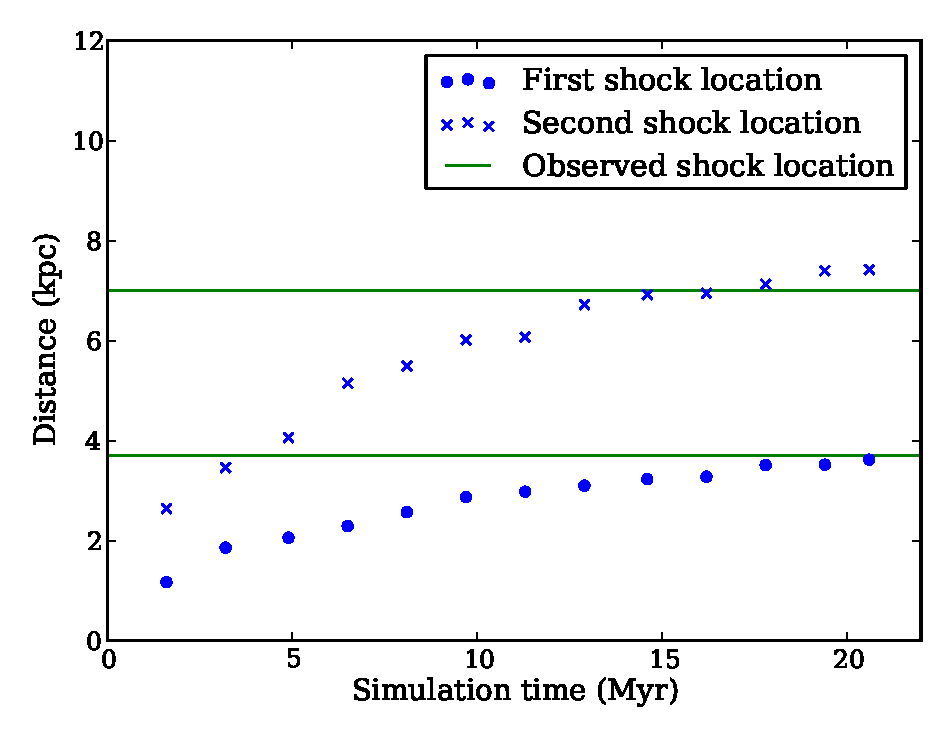
\includegraphics[width=\linewidth]{css.eps}
\caption{
Evolution of the locations of the first (blue dots) and second (blue crosses) shocks with time for run Civ. The horizontal lines represent the observed shock locations. This figure shows that the first two reconfinement shocks move downstream with time and asymptote towards  3.6 and 7.4 kpc at approximately 20 Myr. }
\label{f:s_ev}
\end{figure}

\begin{figure*}
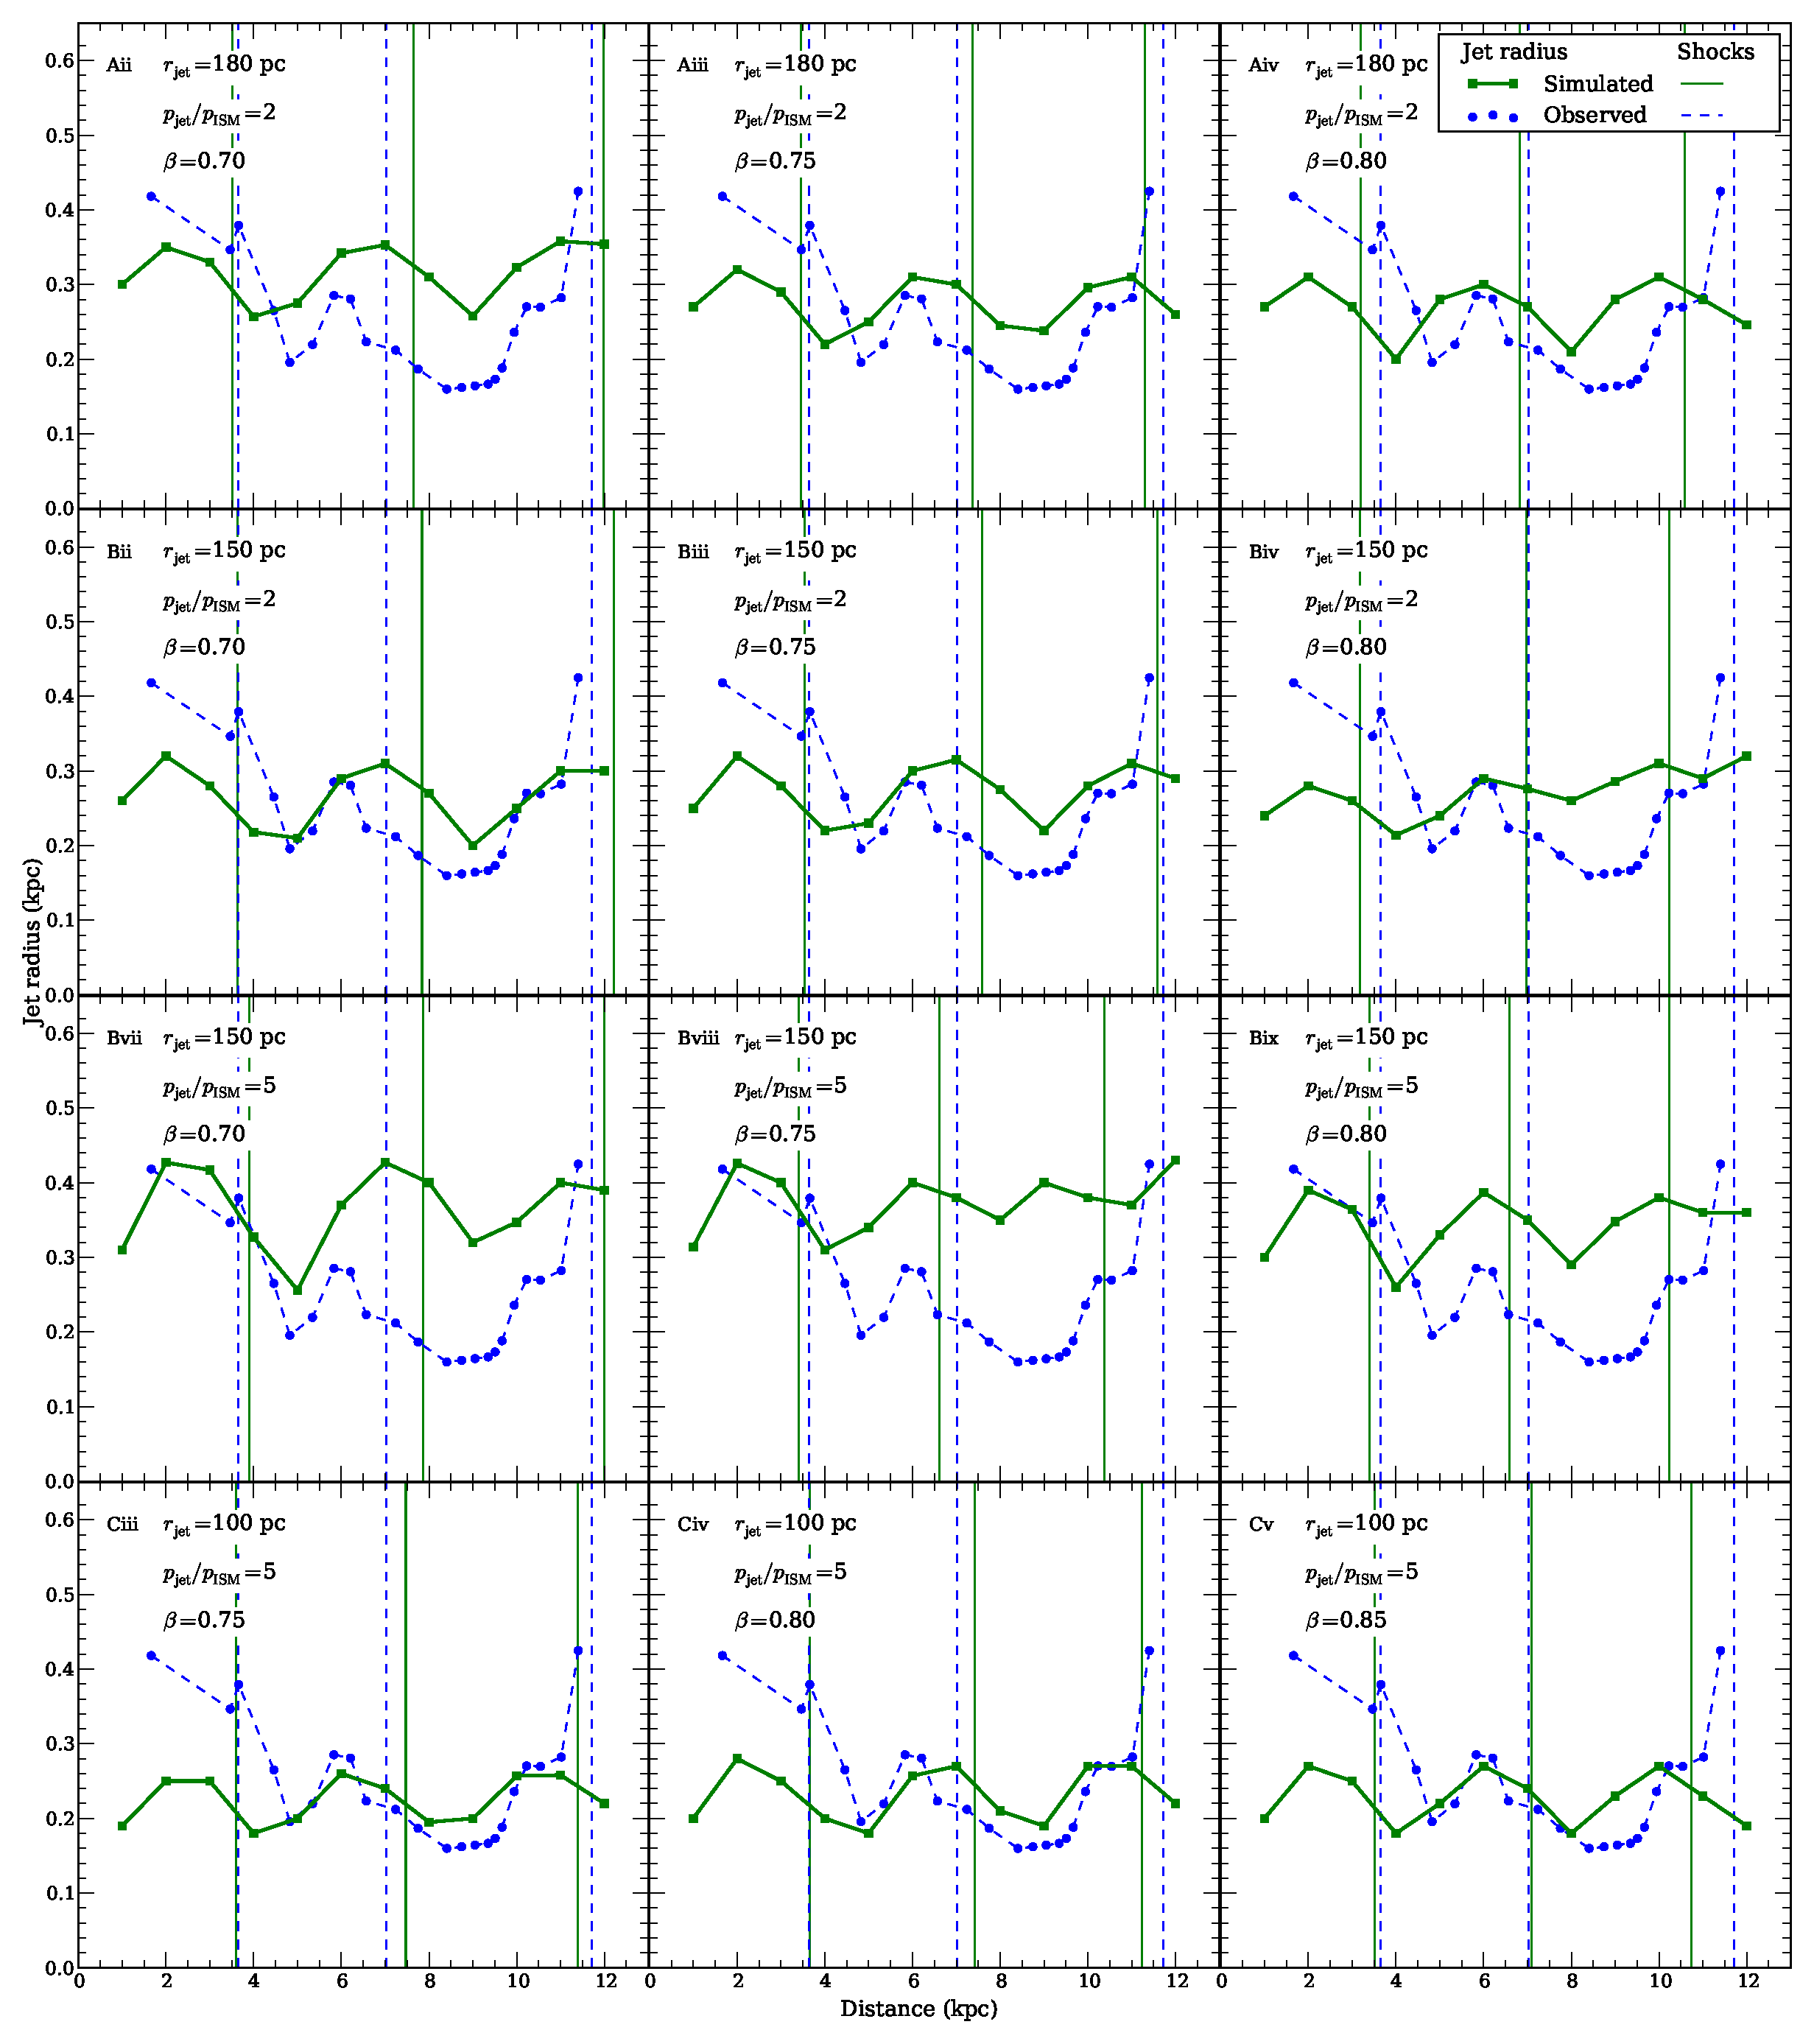
\includegraphics[width=\textwidth]{cmr.eps}
\caption{
Jet radius profiles and shock positions along the jet extracted from selected hydrodynamic simulations. The green line with squares, and the blue lines with circles represent simulated and observation data of radius, respectively. The blue dashed and green solid vertical lines represent the observed and simulated shock locations, respectively. The top row of panels are simulations from set A, the second and third rows of panels are simulations from set B, and the bottom row of panels are simulations from set C. In the simulations shown in the upper two rows of panels, $p_{\rm jet}/p_{\rm ICM}=2$, whereas in those shown in the lower two rows of panels, $p_{\rm jet}/p_{\rm ICM}=2$. The left, middle, and right column of panels, show simulations for which $\beta=0.75$, 0.80, and 0.85, respectively. A visual comparison of the jet radius profiles and shock positions between the simulations and observations shows that, of the models, Ciii, Civ and Cv give the good fit models. }
\label{f:parameter_study}
\end{figure*}

As discussed in \S~\ref{s:model}, the natural wavelength for the occurrence of reconfinement shocks in a supersonic jet is directly related to the jet velocity. I vary the jet velocity, at the same time consistently varying the density parameter $\chi$ to maintain a constant jet kinetic power, noting the location of the first two reconfinement shocks in the jet for each run.
As the cocoon pressure decreases with increasing size the locations of the reconfinement shocks of each run evolve with time. The shocks gradually shift downstream and reach asymptotic values at approximately 20 Myr. I take these asymptotes as the location of the shocks.  Figure~\ref{f:s_ev} shows the evolution of the location of the first (blue dots) and second (blue crosses) shocks with time and the observed location of the shocks (green lines) for run Civ.

The shock positions also vary on a short time scale, oscillating about a mean position.

These variations occur because the pressure field in the backflow adjacent to the jet changes intermittently as a result of the turbulence in the cocoon. Hence, for each run, I have measured the position of the jet shock at five time steps separated by 100 kyr in time. Figure~\ref{f:parameter_study} shows the jet radius profiles and reconfinement shock positions from selected simulations. The results from simulations in set A, B, and C are shown in the top, middle two, and bottom rows, respectively. I compare the simulated shock positions (solid vertical lines) with the observed shocks in Hydra A (dashed vertical lines) and  also compare the simulated jet radius profiles (solid green lines and squares) with the observed jet radius profile (solid blue line and circles).

In assessing these models, one first notes a strong dependence of shock location on jet speed, as expected, and I use this as the first discriminant in selecting candidate best fit models. This narrows the choice to Aiii, Biii, Ciii, Civ, and Cv. Then, focusing on the radius profile, in models Aii, Bii, the jet radius does not contract sufficiently at large distances, which make these two models less appealing. At the same time, I note that the remaining models Cii, Ciii and Civ provide poor radius fits within 3~kpc.  However, the first three data points are derived from a region, which is affected by the emission from the core \citep[see][Fig. 3]{taylor90}. It is also possible that the models do not capture the details of the initial jet-ISM interaction in this region.

Hence, I concentrate on the data points further out from the core. Consequently the choice for the best fit models are Ciii, Civ and Cv. My preference for these three models is based on the fact that the simulated radius shows larger excursions between minima and maxima as exhibited by the data. The parameters for the best fit models Ciii, Civ and Cv are $r_{\rm jet} = 100 \rm pc$, $p_{\rm jet}/P_{\rm ISM} = 5$ and $\beta = 0.75, 0.80, \rm \ and \ 0.85$, respectively. I also note that the last point in the observed radius profile jumps significantly. I attribute this to the onset of turbulence in the jet where it makes a transition to a plume. The third knot/shock may be affected by this transition so that in deciding between models I have mainly concentrated on the first two knots. 

%%%%%%%%%%%%%%%%%%%%%%%%%%%%%%%%%%%%%%%%%%%%%%%%%%%%%%%%%%%%%%%%%%%%
%
%		Northern jet Bright knots
%
%%%%%%%%%%%%%%%%%%%%%%%%%%%%%%%%%%%%%%%%%%%%%%%%%%%%%%%%%%%%%%%%%%%%
\subsection{The surface brightness of the knots in the Northern Jet}
\label{s:knot}

\begin{figure}
\centering
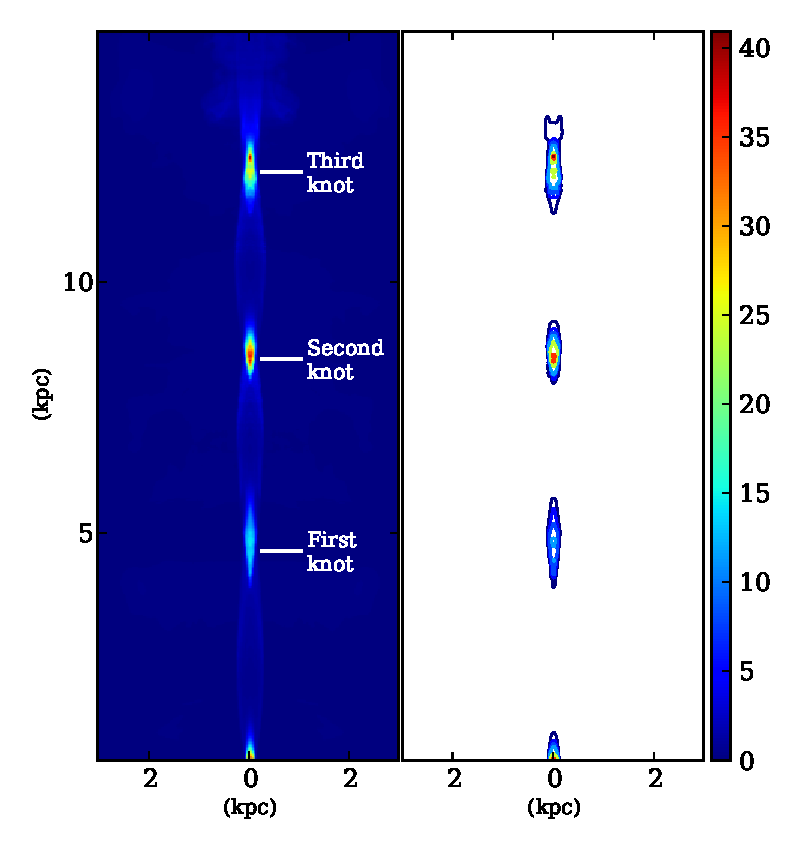
\includegraphics[width=\linewidth]{csb.eps}
\caption{Synthetic surface brightness for model Civ based on an emissivity $j_{\nu} = \delta^{(2+\alpha)} p^{(3+\alpha)/2} \nu^{-\alpha}$, where $\delta= 1/\Gamma(1-\beta \cos 42^\circ)$ is the Doppler factor. The right panel shows the surface brightness contours of the left panel. The contour levels are 4, 8, 11, 14, 25, 35, 40 in arbitrary units.}
\label{radio_morphology}
\end{figure}


To strengthen the association of biconical shocks with the bright knots in the Hydra A northern jet I present a synthetic radio image of one of the best fit models, Ciii, based on an assumed synchrotron emissivity $j_{\nu} \approx {\psi} \, \delta^{2+\alpha} \, p^{(3+\alpha)/2}$, where $\psi$ is the relativistic gas tracer, the Doppler factor $\delta= 1/\Gamma(1-\beta \cos 42^\circ)$ and the pressure dependence assumes that the magnetic pressure is proportional the non-thermal particle pressure \citep[see][\ \S 5.4]{sutherland07a}. Integrated along rays
$I_\nu = \int j_\nu ds$,
 this emissivity provides a semi-quantitative estimate of the surface brightness corresponding to this model.

Fig.~\ref{radio_morphology} (left panel) shows the synthetic surface brightness of the simulated jet. The contour image of the synthetic surface brightness is shown in the right panel. Here I see that, in the shocked zone beyond each biconical shock,  the pressure increases, producing bright knots in each region. This image reproduces some qualitative features of the data: The second and third knots are significantly brighter and more extended than the first knot. However, the 
brightness ratios of the knots are not reproduced. 
Observationally (corrected for resolution) the second knot is 8.7 times brighter than the first and the third knot is 3 times brighter than the second. The model values are 2.5 and 1.14 respectively. In addition, in the observed jet, the FWHM extent of the second knot in the jet direction is 3.3~kpc compared to 0.6~kpc for the model. These differences may possibly be attributed to the approximate magnetic field model, which I have used, or the lack of turbulent three dimensional structure in the simulations. These are aspects to which I can return with three-dimensional simulations with magnetic field. 

%%%%%%%%%%%%%%%%%%%%%%%%%%%%%%%%%%%%%%%%%%%%%%%%%%%%%%%%%%%%%%%%%%%%
%
%		Turbulent Transition
%
%%%%%%%%%%%%%%%%%%%%%%%%%%%%%%%%%%%%%%%%%%%%%%%%%%%%%%%%%%%%%%%%%%%%
\subsection{Transition to turbulence}
\begin{figure*}
\centering
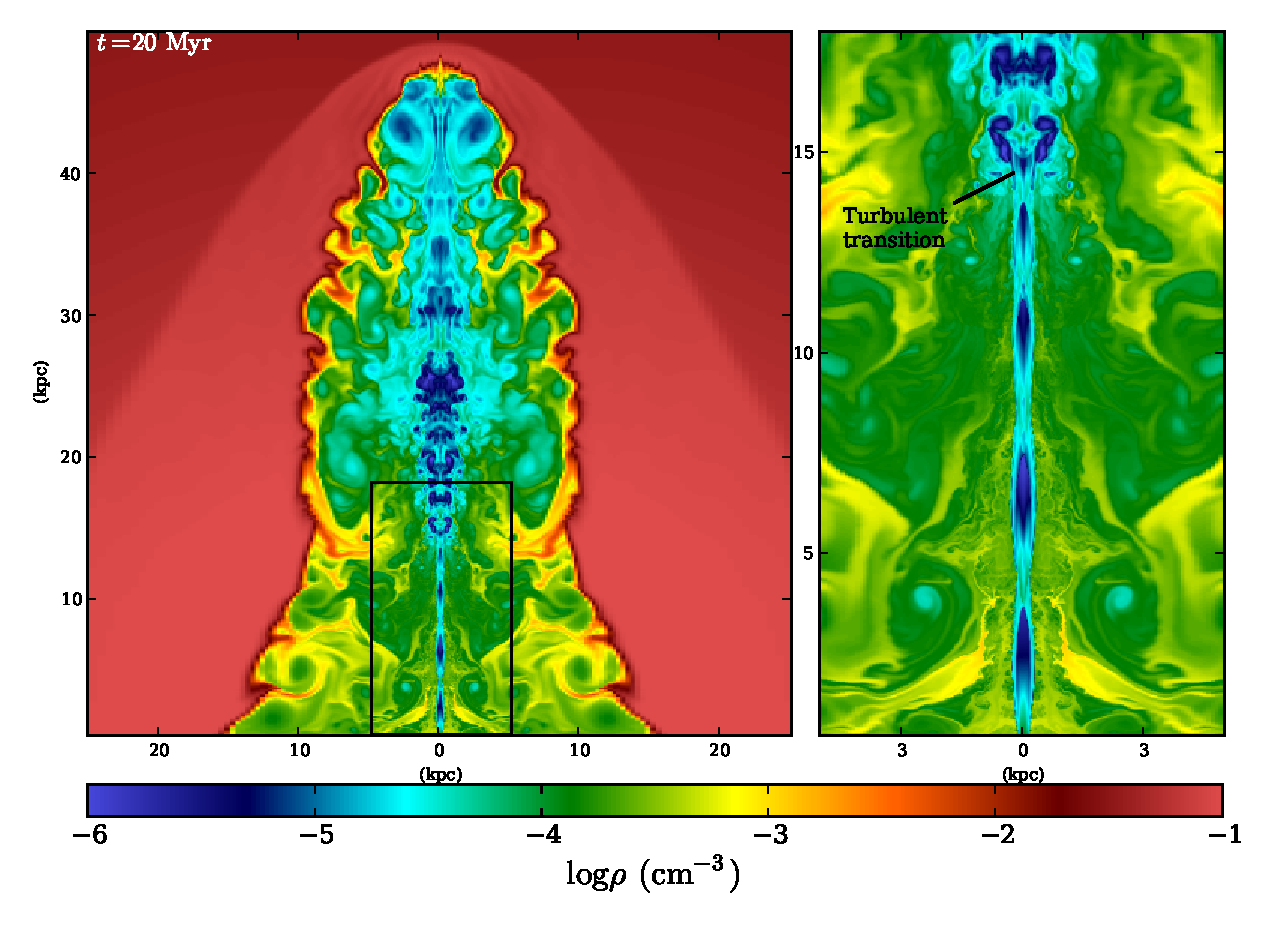
\includegraphics[width=\textwidth]{cbm.eps}
\caption{Logarithmic density snapshot for run Civ at $t=20\,\mathrm{Myr}$ in the left panel. The right panel shows the zoomed in central zone marked with black rectangle in the left panel. This is one of the best fit models, which yields the correct location of the first two biconical reconfinement shocks in the northern jet of Hydra A. A transition to turbulence occurs due to significant shock deceleration of the jet in the reconfinement shocks and the developing Kelvin-Helmholtz instability. }
\label{t_trans}
\end{figure*}
 
 \begin{figure}
\centering
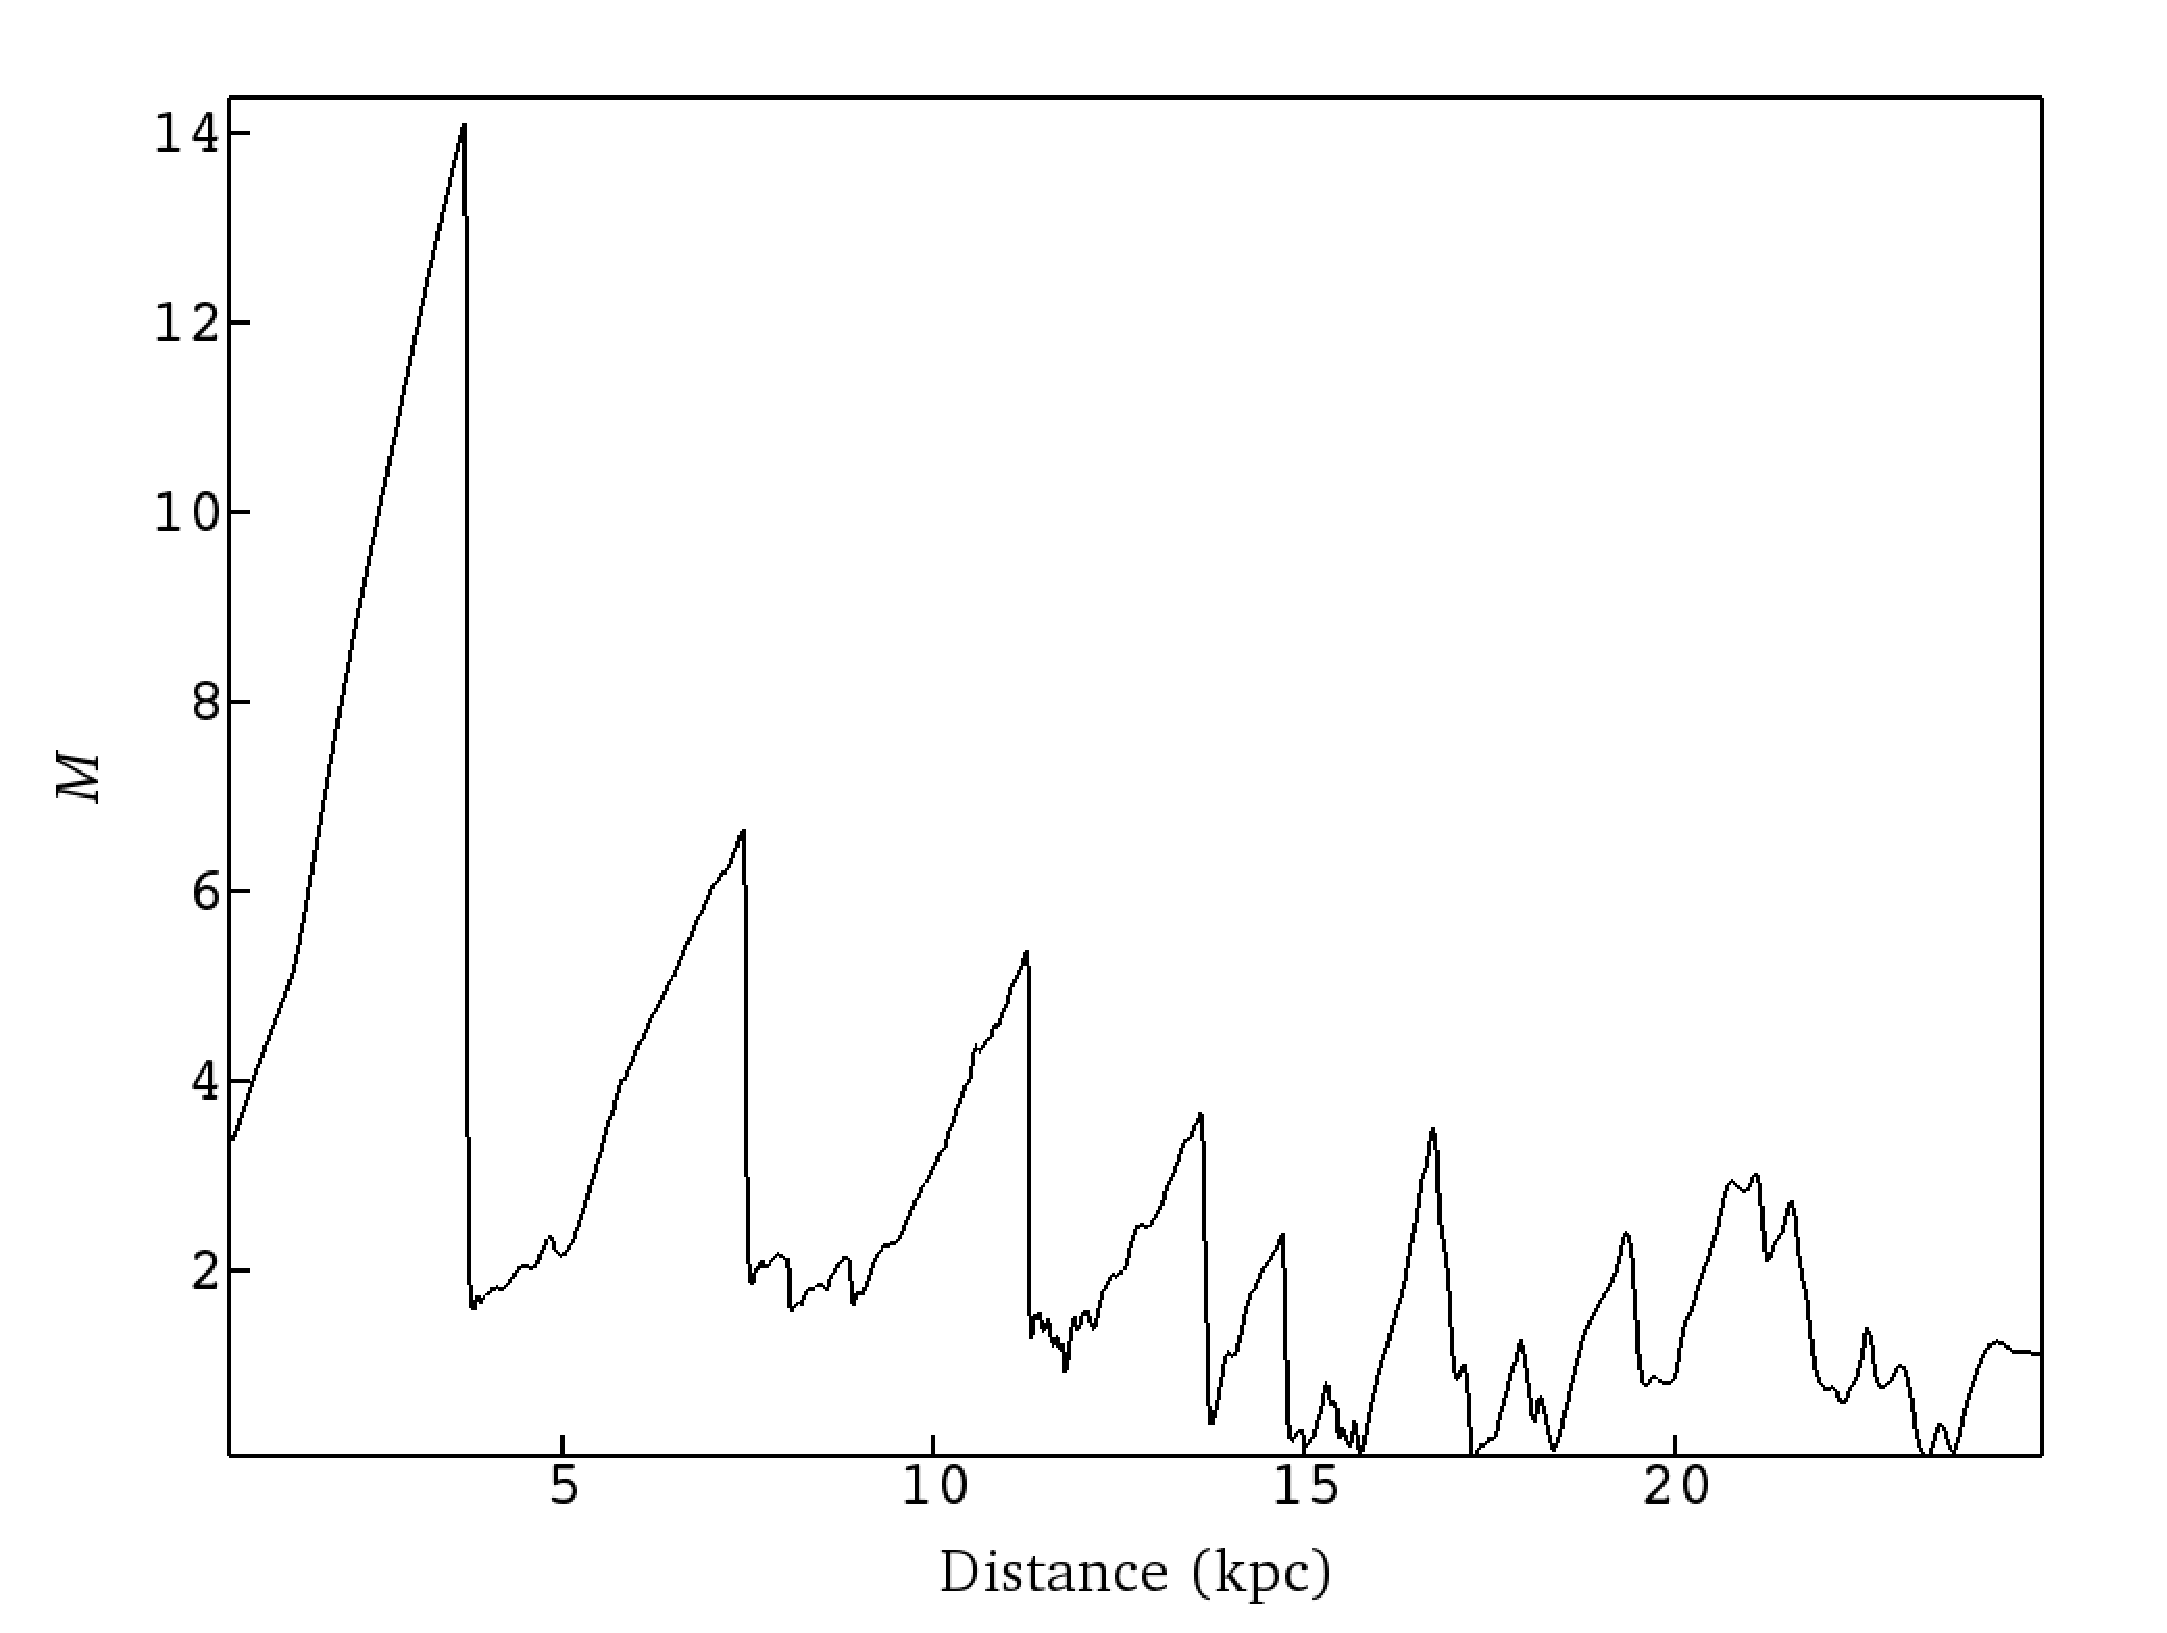
\includegraphics[width=\linewidth]{cml.eps}
\caption{The Mach number of the jet of model Civ at different locations along the jet axis.}
\label{mach}
\end{figure}
 

These two-dimensional models cannot adequately reproduce the structure of the entire source, in particular the plume like regions beyond approximately $7.4^{\prime\prime}$. These are probably the result of three-dimensional turbulence and/or precession, and these effects will be addressed in future study of three dimensional precessing jet model. However, I note that the numerical models \emph{qualitatively} reproduce the turbulent transition of the jets to plumes, albeit at a distance of 14~kpc compared to approximately 11 kpc deprojected in Hydra~A. In the density image snapshot at approximately 20 Myr of run Civ, Fig.~\ref{t_trans} (the left panel shows the full computational domain and the right panel is the zoom in section indicates by the rectangle in the left panel), a series of biconical  shocks appears in the jet.  Deceleration of the jet occurs at these shocks and the jet becomes subsonic after the fourth shock at $\sim 14 \rm \ kpc$ (see the variation of Mach number of the flow with distance along the jet axis in Fig.~\ref{mach}). Beyond 14~kpc the jet transitions to turbulence as a result of the axisymmetric Kelvin-Helmholtz instability, which becomes stronger as the Mach number decreases.) 
Although the axisymmetric jet simulations shed some light on the turbulent transition of the jet, it is well known that turbulence and the formation of plumes are three dimensional phenomena, especially in supersonic flows. I study the details of these features of the inner 20 kpc of the Hydra A jets in the ensuing three dimensional study.


%%%%%%%%%%%%%%%%%%%%%%%%%%%%%%%%%%%%%%%%%%%%%%%%%%%%%%%%%%%%%%%%%%%%
%
%		Brightness Ratio
%
%%%%%%%%%%%%%%%%%%%%%%%%%%%%%%%%%%%%%%%%%%%%%%%%%%%%%%%%%%%%%%%%%%%%

\subsection{Brightness ratio of the jets} \label{s:b_r}
 \begin{figure*}
\centering
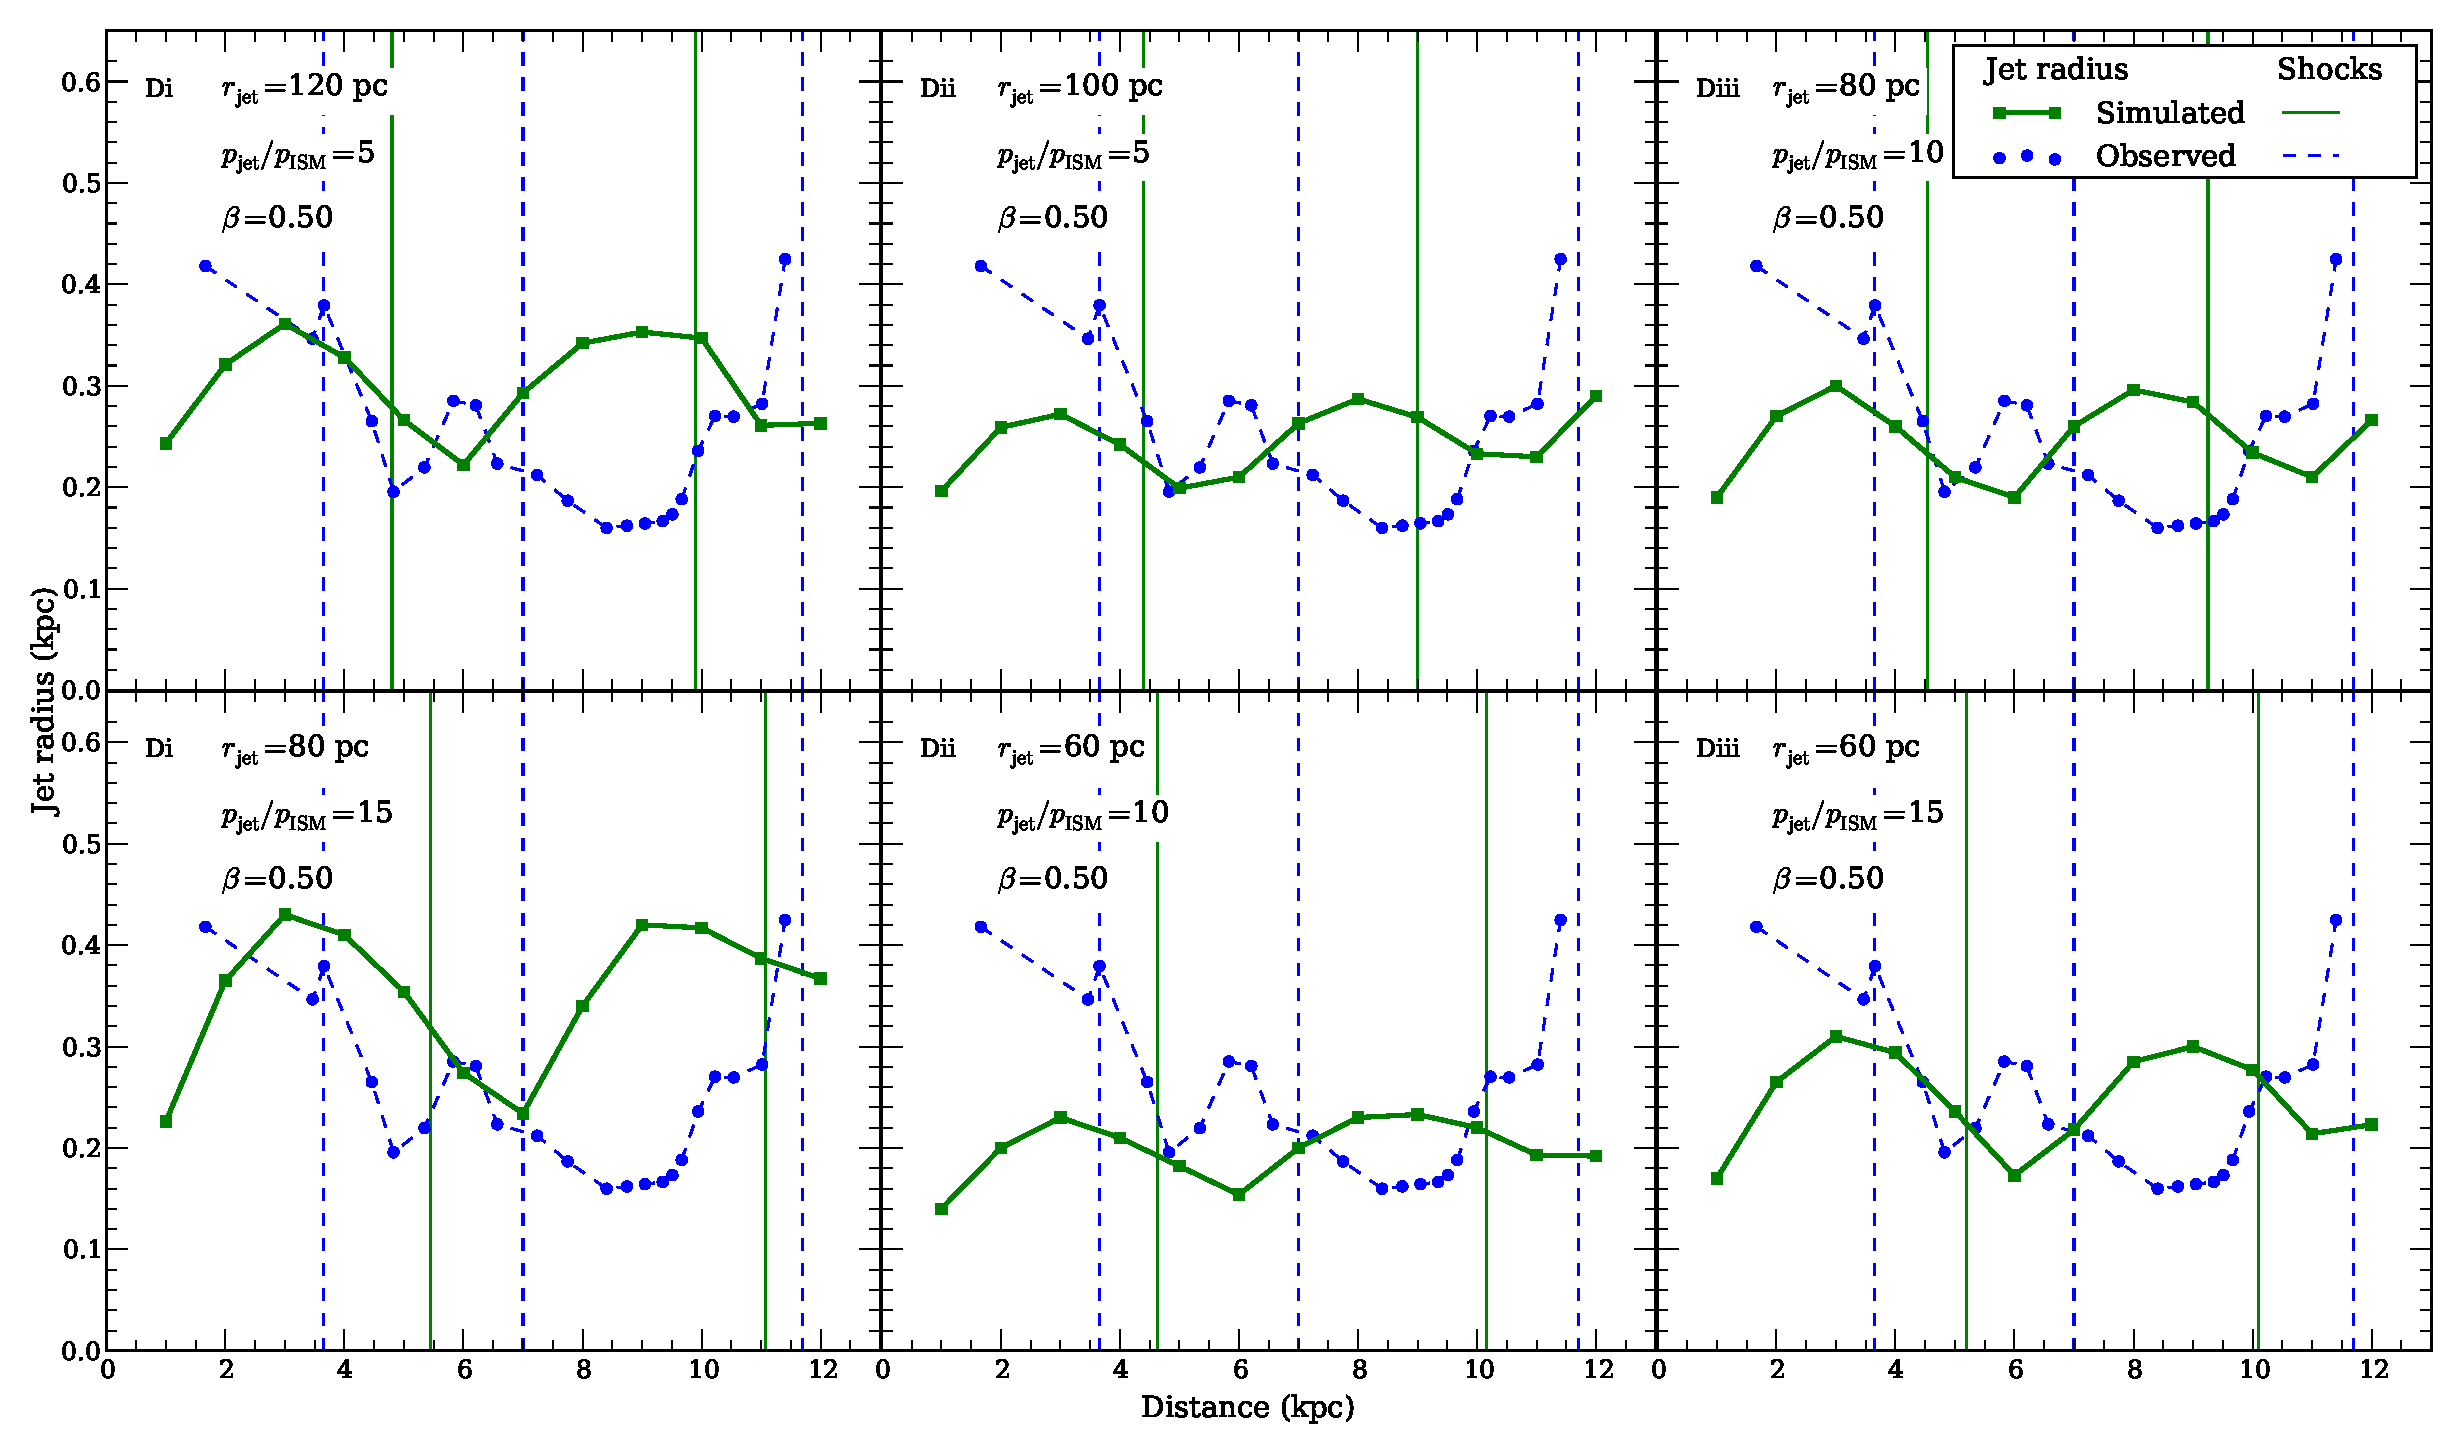
\includegraphics[width=\textwidth]{clv.eps}
\caption{Jet radius profile and shock positions along the jet for jet velocity 0.5. The green line with squares, and the blue lines with circles represent simulated and observation data of radius, respectively. The blue dashed and green solid vertical lines represent the observed and simulated shock locations, respectively.}
\label{f:p_s_b5}
\end{figure*}



I have used the 6cm VLA data of \citet{taylor90} to determine the flux density ratio of the northern and southern jets within the first 10 kpc, obtaining  a value $\approx 7.0$\footnote{\citet{taylor90} quote a value of 1.9, which is close to the observed ratio within 1~kpc.} Attributing this ratio to Doppler beaming, and using the inclination estimated by \citet{taylor90}, implies a moderately relativistic jet  $\beta \approx  0.5$. However, my parameter space study produces a higher jet velocity $\sim 0.8$ which, on the basis of a simple estimate, would give a brightness ratio $\approx 40$. However, in my model, the emissivity is dominated by the decelerated post-shock regions of the jet, so that I estimate the brightness ratio from the synthetic brightness images of approaching and receding jets. With this approach, I obtain a simulated flux density ratio of 33 which still differs significantly from the observed value by a factor $\approx 5$.

I ran several additional models with jet $\beta = 0.5$,  different jet inlet radii 120~pc, 100~pc, 80~pc and 60~pc and different pressure ratio 5, 10, and 15, keeping the jet kinetic power constant at $10^{45} \rm \ ergs \ s^{-1}$. I have not decreased the jet radius below 60~pc because that would require an even more highly over pressured jet to obtain the correct radius profile. These $\beta=0.5$ models are summarised in Table~\ref{t:sim_par} (set D) and the comparison of the simulated and observed shock positions and radius profiles are shown in Fig.~\ref{f:p_s_b5}. It is evident that no model with the given jet kinetic power and jet $\beta = 0.5$ is able to produce good fits for both the shock position and the jet radius. The shock spacings are all significantly larger than the observed shock spacing and the radius profiles are mismatched with these models. 

From the above I can say that if I fix the inclination angle at the \citet{taylor90} value of $42^\circ$ and fix the jet kinetic power at $10^{45} \rm \ ergs \ s^{-1}$, then the jet pressure, jet velocity and the inlet jet radius at 0.5~kpc away from the core of the Hydra A northern jet are well-constrained by both the jet radius profile and the first two knot/shock spacings. The best-fit values are $\beta = 0.75 - 0.85$ and $r_j = 100 \> \rm pc$. Thus, there is a discrepancy in the flux density ratio between the simulated and observed jets. Two potential explanations of the low flux density ratio are: i) Since my models do not include the magnetic field, I employ the assumption $p\propto B^2/8\pi$ which gives a brightness ratio 33. If I further assume that the magnetic field is 2.5 times stronger in the southern jet of Hydra A I would obtain a lower brightness ratio $\sim 7$. ii) The southern jet is more dissipative since it is more twisted and produces more shocks producing a larger intrinsic emissivity than the northern jet. 


%%%%%%%%%%%%%%%%%%%%%%%%%%%%%%%%%%%%%%%%%%%%%%%%%%%%%%%%%%%%%%%%%%%%
%
%		Variation in the inclination angle
%
%%%%%%%%%%%%%%%%%%%%%%%%%%%%%%%%%%%%%%%%%%%%%%%%%%%%%%%%%%%%%%%%%%%%
\subsection{Variation of the inclination angle}\label{s:theta}

 \begin{figure}
\centering
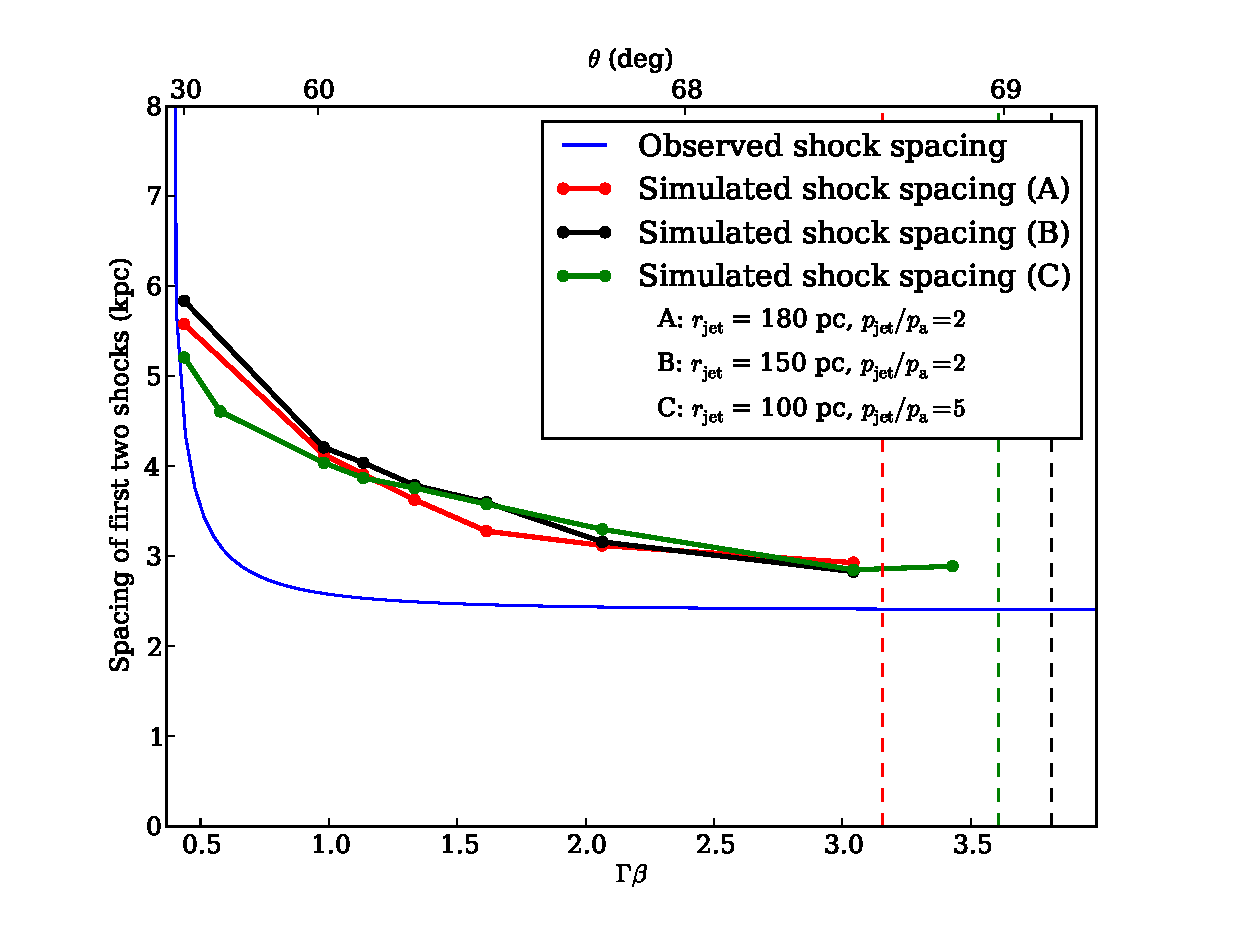
\includegraphics[width=\linewidth]{cts.eps}
\caption{Comparison of the observed  spacing  of the first two shocks (blue curves) with the corresponding simulated shock spacing (red points for model set A, black points for model set B, and green points for model set C) as a function of the 4-velocity $\Gamma \beta$. The dashed vertical lines represent the upper limits of $\Gamma \beta$ for each model (set A -- red, set B -- black, and set C -- green). These limits are estimated for $\chi = 0$ using Eqn.~(\ref{chi2}).}
\label{f:ss}
\end{figure}

In the above models I have used the angle between the jet and the line of sight, $\theta \approx 42^\circ$, estimated by \citet{taylor93} from the rotation measure asymmetry of Hydra~A. However, there is a fairly large uncertainty in their estimate of $\theta$ with $30^\circ \leq \theta \leq 60^\circ$. Increasing $\theta$ from $42^{\circ}$, would reduce the brightness ratio? However, for larger inclinations, the deprojected knot separation would decrease, and as I have seen with the above models, this would require a higher velocity than $0.8 \rm c$, tending to \emph{increase} the brightness ratio. Similar considerations apply if I \emph{decrease} the inclination. Nevertheless, is it possible that notwithstanding opposing effects, an inclination angle within the \citet{taylor90} range, and a jet velocity, can be found that are consistent with the dual constraints of surface brightness ratio and projected knot spacing? 

In order to assess this possibility I adopted the following procedure: For $\beta$ within the range, $0.35 < \beta < 0.98$ (the lower limit being defined by the brightness ratio, $R=7$) I first estimate the value of $\theta$ corresponding to $R = 7$, using the standard Doppler beaming formula, $\theta (\beta)= \beta^{-1}(R^{1/2.7}-1)(R^{1/2.7}+1)^{-1}$. For these values of $\theta(\beta)$ I determine the deprojected spacing between the first two shocks $D_{1,2}(\beta) = 2.25 /\sin \theta(\beta) \> \rm kpc$ given the observed spacing of 2.25~kpc. This is shown, as a function of the 4-velocity, $\Gamma \beta$, as the blue curve in Fig.~\ref{f:ss}. I then compare the observed deprojected knot spacings with the values inferred from the simulations so that in Fig.~\ref{f:ss} the simulated shock spacing, for model sets A, B and C, are also plotted as functions of $\Gamma \beta$. The upper limits on the 4-velocity for each model (estimated from Eqn.~(\ref{chi2})), associated with a zero density parameter, $\chi = 0$, are also shown as dashed vertical lines. 


The first point to note with this comparison is that for most of allowable range of $\beta$ Fig.~\ref{f:ss} shows that the calculated shock spacing exceeds the observed, deprojected value. At the upper end of the $\beta$ range the simulated shock spacings for each model asymptote to $\approx 2.85$ kpc for values of $\Gamma \beta \gtrsim 3$, i.e., $\beta \gtrsim 0.95$. However the asymptote of the observed shock spacing $\approx 2.4$ kpc. Hence, there is an offset of approximately 0.5~kpc between the asymptotes of the simulated and observed shock spacing for $\Gamma \beta \gtrsim 3$.  

At the other end of the allowable range of velocity, $\beta \approx 0.345$ ($\Gamma \beta = 0.368$), it could be inferred that the simulations and observations intersect at approximately this limiting value. However, this is the result of the steepness at $\beta \approx 0.345$ of the (blue) curve representing the observed deprojected shock spacing as a function of 4-velocity, rather than a real physical correspondence between observed and simulated values. It would be fortuitous if the jet initial velocity were to be almost exactly the same as the lower limit on the jet velocity implied by beaming. Hence I reject a solution at this end of the $\beta$ range on the basis of the ``fine-tuning'' that would be involved in accepting it. Another unappealing feature of a low-$\beta$ solution is that the jet would be initially heavy with $\chi \gtrsim 300$. 
As I noted above, observations and modelling of X-ray observations of the lobes of radio galaxies indicate that jets are initially electron-positron in composition \citep{croston05a,croston14} and $\chi \gtrsim 300$ is inconsistent with this. 
 
Another way of looking at the issue of reconciling shock spacing and flux ratios is the following: Consider the simulation points near the upper end of the $\beta$ range in Fig.~\ref{f:ss}, where the discrepancy between the observed jet and simulated jets with $\chi \sim 1$ is the least. By way of example, consider the (green) point in simulation series C with $\beta=0.95$ ($\Gamma \beta = 3.04$). The simulated flux ratio (see \S~\ref{s:b_r}) for this model is 26.5, a factor of 3.8 higher than the observed value. Thus, even for these models there is an implication of intrinsic differences in the northern and southern jet rest-frame emissivities. Moreover, this ratio is not very different from the value of 33 for the $\beta =0.8$, $\theta = 42^\circ$ model considered earlier.

In view of the above, I conclude that, taking into account the modelling of shock spacing, radius evolution and surface brightness ratios, the most likely situation is that of fast, $\beta \gtrsim 0.8$, jets with an intrinsic difference between the rest-frame emissivities of northern and southern jets.

%%%%%%%%%%%%%%%%%%%%%%%%%%%%%%%%%%%%%%%%%%%%%%%%%%%%%%%%%%%%%%%%%%%%%%%%%
%% 
%%												Further implication of axisymmetric model 
%%
%%%%%%%%%%%%%%%%%%%%%%%%%%%%%%%%%%%%%%%%%%%%%%%%%%%%%%%%%%%%%%%%%%%%%%%%%
%\section{A verification of the axisymmetric model: naked jet}
%The simulations of jets propagating into the cluster atmosphere conducted in the previous two chapters typically evolve for 50 kpc, which is the extent of the simulation domain, over a timescale of approximately 20~Myr. While the shock structures in the jet, the turbulent transition of the jet, and global structures, e.g. the turbulent backflows in the cocoon and forward shock of the bubble, are well captured, the simulation time is less than the age of the source. It is possible therefore that the jet is being affected by the backflow within this restricted domain. The purpose of this chapter, therefore, is to ascertain whether the shock positions seen in the simulations are unaffected by the back flow form the head of the jet. To this end I look at the evolution of the shock positions with time, and also perform a simulation of an unbounded jet -- a jet spanning the entire domain and not bounded by a termination shock. This is more representative of conditions in the inner regions of an evolved radio source, such as that of Hydra A. 
%
%%The simulations of jets propagating into the cluster atmosphere conducted above typically evolve to an extent of 50 kpc, as restricted by the simulation domain, over a timescale of approximately 20~Myr. While the shock structures in the jet, the turbulent transition of the jet, and global structures, e.g. the turbulent backflows in the cocoon and forward shock of the bubble, are well captured, the simulation time is less than the age of the source. I therefore need to ascertain whether the shock positions seen in the simulations are likely to approach asymptotic values with time. To this end I look at the evolution of the shock positions with time, and also perform a simulation of an unbounded jet -- a jet spanning the entire domain and not bounded by a termination shock, which is more representative of conditions in the inner regions of an evolved radio source, such as that of Hydra A. 
%
%\subsection{Simulation results} \label{s:jet_stream}
%\begin{figure}
%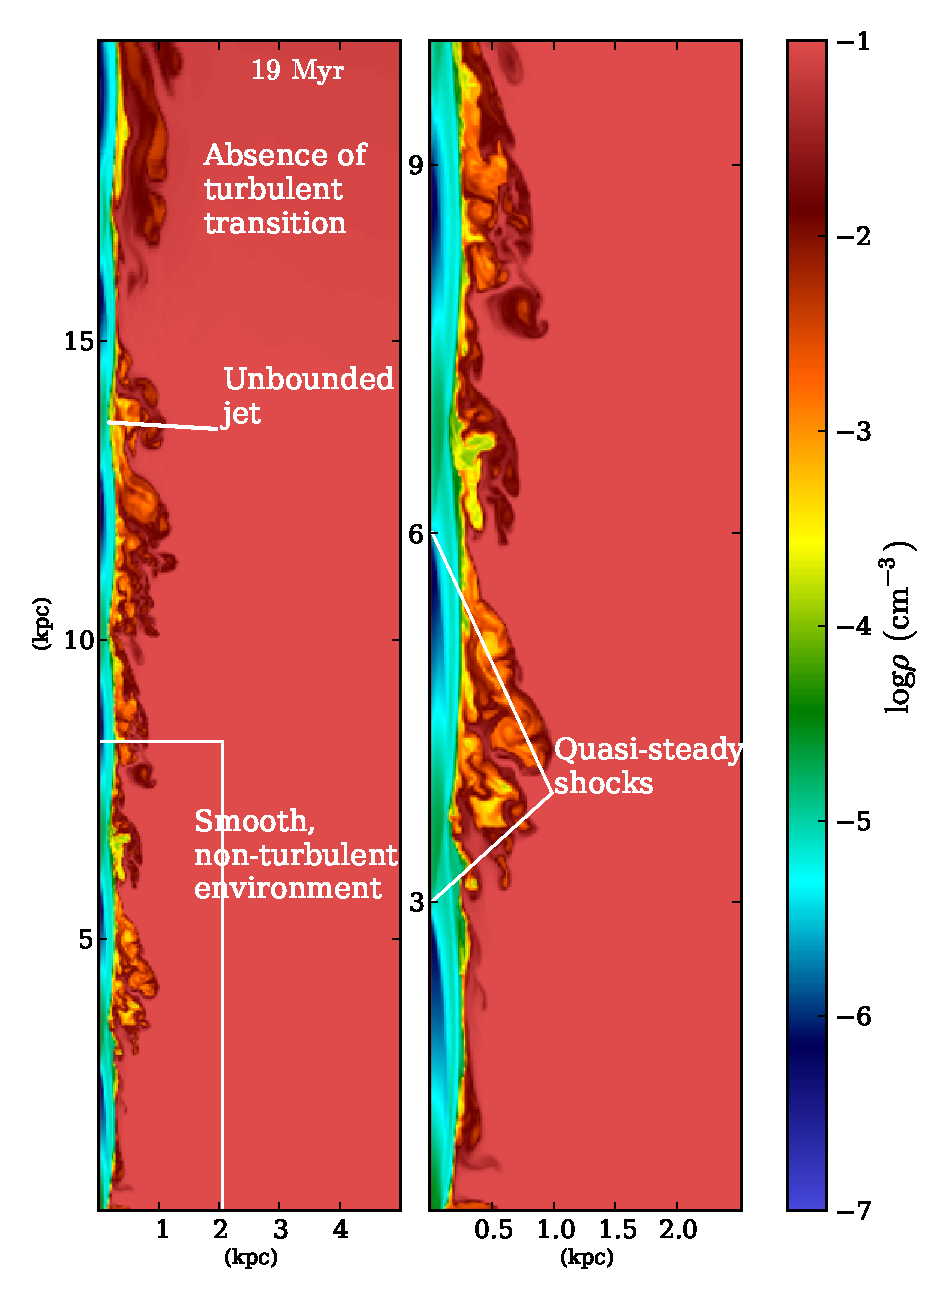
\includegraphics[width=\linewidth]{njm.eps}
%\caption{Logarithmic density image of a simulation of the interaction of an unbounded jet with a non-turbulent ICM. The shock positions are almost time-independent as the jet expands and reconfines multiple times before escaping through the top boundary. No transition to turbulent flow is observed. The right panel is a closeup of the central region marked with a box in the left panel. In both panels the scales are in kpc.}
%\label{f:u_jet}
%\end{figure}
%
%\begin{figure}
%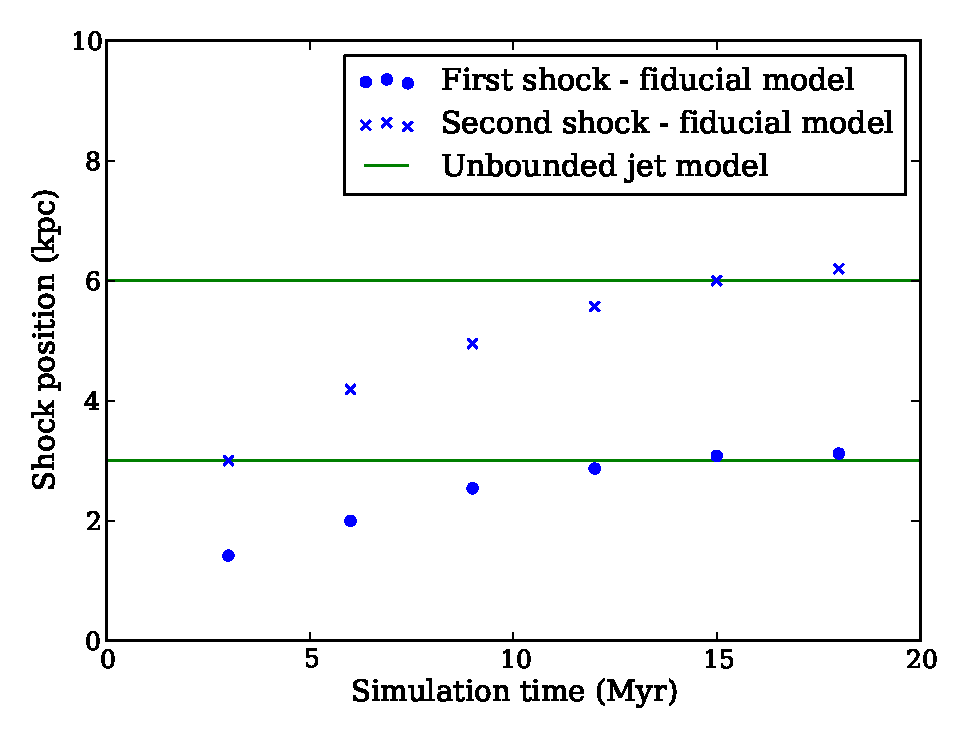
\includegraphics[width=\linewidth]{nse.eps}
%\caption{Evolution of the reconfinement shock positions with time for model Cvii. The circles and crosses represent the first and second shock locations, respectively. The horizontal lines mark the shock positions obtained in the simulation of an unbounded jet using the same parameters as those in model Cvii.}
%\label{f:c_vs_n}
%\end{figure}
%
%Figure~\ref{f:c_vs_n} shows the evolution of the first (circles) and second (crosses) shock positions for model Cv, respectively, as a function of time. The shock positions increase with time, but appear to asymptote to values very close to 3 and 6 kpc, respectively.
%
%In the simulation of an unbounded jet, I set up the the jet inlet with the same jet parameters and geometry as in run Cv, but I also initiate the full extent of a jet column spanning the length of the domain along the jet axis at the start of the simulation. Since the jet is initially overpressured, it expands and contracts, sending a nearly axisymmetric shock wave into the ambient medium, and forming reconfinement shocks along the jet axis. Kelvin-Helmholtz instabilities develop in the shear layer between the jet and the ambient medium, but other than that and the initial adjustment, the flow in the entire simulation box is broadly time-independent. Without a jet backflow, a turbulent cocoon does not develop. Simulations of unbounded jet allow us to measure the quasi-steady reconfinement shock positions because, in the absence of a turbulent cocoon, the global structure of the flow in the simulation domain and the pressure field of the medium surrounding the jet remain fairly steady.
%
%Figure~\ref{f:u_jet} shows the features developed by an unbounded jet model at time $t=19$ Myr. The right panel shows a closeup of the in central $5\times20$ kpc region. The jet is embedded in a relatively steady ambient medium exhibits the first two reconfinement shocks at 3 and 6 kpc. This result is also shown in Fig.~\ref{f:c_vs_n} with two horizontal lines. These shock locations agree with the asymptotic values of the shock position in run Ciii. 
%
%Simulations of unbounded jets are useful for accurately measuring nearly time-independent positions of shocks in a jet, provided the top outflowing boundary is not affecting the structure of the jet. However, these models are not useful in explaining other important features of the Hydra A northern jet, in particular, the turbulent transition of the jet and the formation of the plume structure. As we see in the unbounded jet simulation the deceleration through the biconical shocks and the entrainment in the shear layer alone can not produce the turbulent transition. The ram pressure of the turbulent back flow in the cocoon plays an important role in further deceleration and disruption of the jet, which we see in the simulations of an evolving jet, in which the jet is surrounded by a cocoon of entrained plasma. 
%
%


\chapter{A verification of the axisymmetric model: model of a naked jet}\label{chapter6}
%%%%%%%%%%%%%%%%%%%%%%%%%%%%%%%%%%%%%%%%%%%%%%%%%%%%%%%%%%%%%%%%%%%%%%%%
% 
%												Further implication of axisymmetric model 
%
%%%%%%%%%%%%%%%%%%%%%%%%%%%%%%%%%%%%%%%%%%%%%%%%%%%%%%%%%%%%%%%%%%%%%%%%
%\section{A verification of the axisymmetric model: naked jet}
The simulations of jets propagating into the cluster atmosphere conducted in the previous two chapters typically evolve for 50 kpc, which is the extent of the simulation domain, over a timescale of approximately 20~Myr. While the shock structures in the jet, the turbulent transition of the jet, and global structures, e.g. the turbulent backflows in the cocoon and forward shock of the bubble, are well captured, the simulation time is less than the age of the source. It is possible therefore that the jet is being affected by the backflow within this restricted domain. The purpose of this chapter, therefore, is to ascertain whether the shock positions seen in the simulations are unaffected by the back flow form the head of the jet. To this end I look at the evolution of the shock positions with time, and also perform a simulation of an unbounded jet -- a jet spanning the entire domain and not bounded by a termination shock. This is more representative of conditions in the inner regions of an evolved radio source, such as that of Hydra A. 

%The simulations of jets propagating into the cluster atmosphere conducted above typically evolve to an extent of 50 kpc, as restricted by the simulation domain, over a timescale of approximately 20~Myr. While the shock structures in the jet, the turbulent transition of the jet, and global structures, e.g. the turbulent backflows in the cocoon and forward shock of the bubble, are well captured, the simulation time is less than the age of the source. I therefore need to ascertain whether the shock positions seen in the simulations are likely to approach asymptotic values with time. To this end I look at the evolution of the shock positions with time, and also perform a simulation of an unbounded jet -- a jet spanning the entire domain and not bounded by a termination shock, which is more representative of conditions in the inner regions of an evolved radio source, such as that of Hydra A. 

\subsection{Simulation results} \label{s:jet_stream}
\begin{figure}
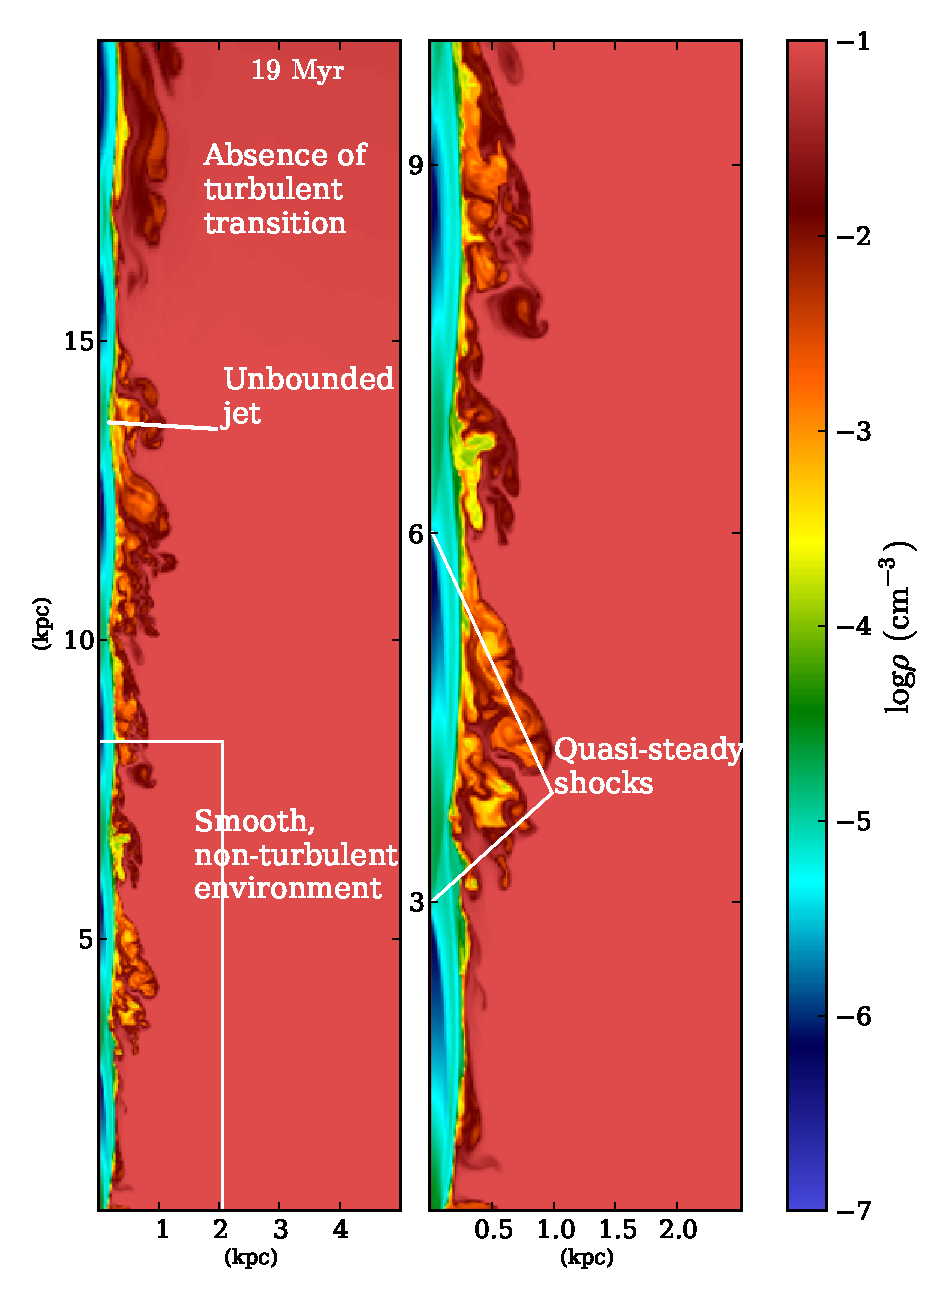
\includegraphics[width=\linewidth]{njm.eps}
\caption{Logarithmic density image of a simulation of the interaction of an unbounded jet with a non-turbulent ICM. The shock positions are almost time-independent as the jet expands and reconfines multiple times before escaping through the top boundary. No transition to turbulent flow is observed. The right panel is a closeup of the central region marked with a box in the left panel. In both panels the scales are in kpc.}
\label{f:u_jet}
\end{figure}

\begin{figure}
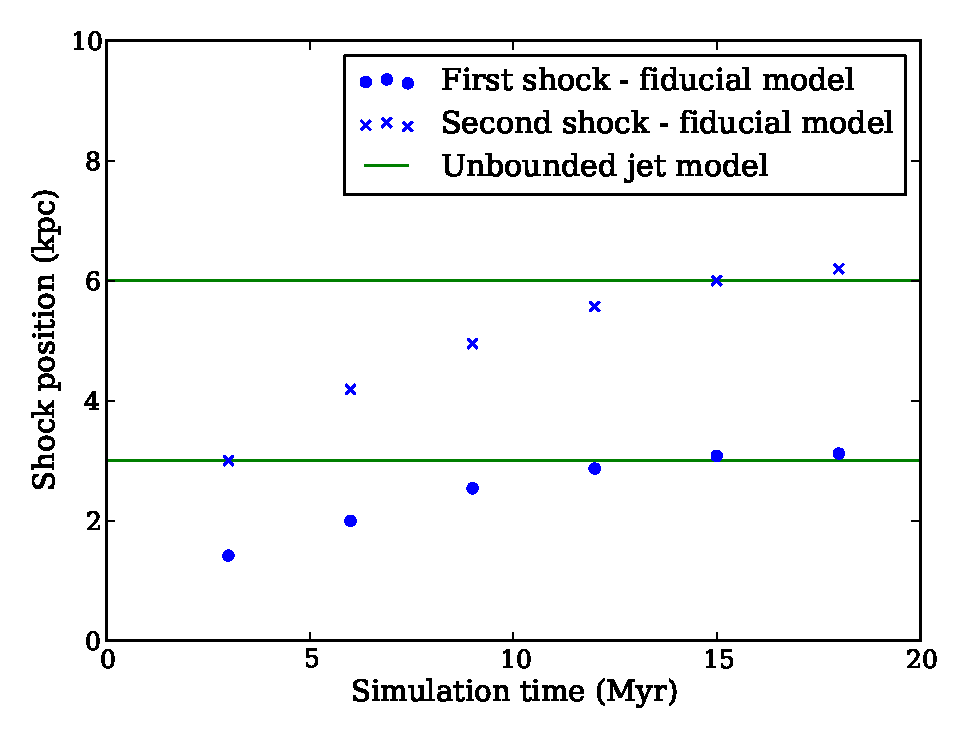
\includegraphics[width=\linewidth]{nse.eps}
\caption{Evolution of the reconfinement shock positions with time for model Cvii. The circles and crosses represent the first and second shock locations, respectively. The horizontal lines mark the shock positions obtained in the simulation of an unbounded jet using the same parameters as those in model Cvii.}
\label{f:c_vs_n}
\end{figure}

Figure~\ref{f:c_vs_n} shows the evolution of the first (circles) and second (crosses) shock positions for model Cv, respectively, as a function of time. The shock positions increase with time, but appear to asymptote to values very close to 3 and 6 kpc, respectively.

In the simulation of an unbounded jet, I set up the the jet inlet with the same jet parameters and geometry as in run Cv, but I also initiate the full extent of a jet column spanning the length of the domain along the jet axis at the start of the simulation. Since the jet is initially overpressured, it expands and contracts, sending a nearly axisymmetric shock wave into the ambient medium, and forming reconfinement shocks along the jet axis. Kelvin-Helmholtz instabilities develop in the shear layer between the jet and the ambient medium, but other than that and the initial adjustment, the flow in the entire simulation box is broadly time-independent. Without a jet backflow, a turbulent cocoon does not develop. Simulations of unbounded jet allow us to measure the quasi-steady reconfinement shock positions because, in the absence of a turbulent cocoon, the global structure of the flow in the simulation domain and the pressure field of the medium surrounding the jet remain fairly steady.

Figure~\ref{f:u_jet} shows the features developed by an unbounded jet model at time $t=19$ Myr. The right panel shows a closeup of the in central $5\times20$ kpc region. The jet is embedded in a relatively steady ambient medium exhibits the first two reconfinement shocks at 3 and 6 kpc. This result is also shown in Fig.~\ref{f:c_vs_n} with two horizontal lines. These shock locations agree with the asymptotic values of the shock position in run Ciii. 

Simulations of unbounded jets are useful for accurately measuring nearly time-independent positions of shocks in a jet, provided the top outflowing boundary is not affecting the structure of the jet. However, these models are not useful in explaining other important features of the Hydra A northern jet, in particular, the turbulent transition of the jet and the formation of the plume structure. As we see in the unbounded jet simulation the deceleration through the biconical shocks and the entrainment in the shear layer alone can not produce the turbulent transition. The ram pressure of the turbulent back flow in the cocoon plays an important role in further deceleration and disruption of the jet, which we see in the simulations of an evolving jet, in which the jet is surrounded by a cocoon of entrained plasma. 



\chapter{Axisymmetric model for the southern jet}
\label{chapter8}

%\textbf{(b)} Zoom-in of the top rectangular region in a) showing the bright knots in the northern jet. Contours are at 1.5, 2.7, 3.7, 5.1, 6.3, 7.5, 8.8, 10, 21, 37, 51, 72, 90, 103, 154, 311, and 466 mJy arcsec$^{-2}$. \textbf{(c)} Zoom-in of the bottom rectangular region in a) showing the bright knots in the southern jet. Contours are at 1.5, 2.0, 2.2, 2.7, 3.7, 5.1, 5.5, 6.0, 6.3, 6.8, 7.5, 8.8, 10, 21, 37, 51,  72, 90, 103, 154, 311, and 466 mJy arcsec$^{-2}$.

In chapter~\ref{chapter5} I presented the detail study of the Hydra A northern jet focussing two bright knots and the radial oscillation of the central 10~kpc jet. Here I consider the implications of the knot structure in the southern jet. In this case there are \emph{four} knots compared to two in the northern jet and the jet is more curved. Moreover there has been no determination of the jet radius versus distance from the core. Hence, the southern jet data do not provide as good a basis for parameter estimation. Nevertheless, it is of interest to apply the previous approach, which reinforces the velocity estimates for the northern jet. There is one interesting difference in that the optimal model has an initial overpressure ratio of unity. Four bright knots and the locations of the associated reconfinement shocks are shown in Fig.~\ref{southern}.

\begin{figure}
\centering
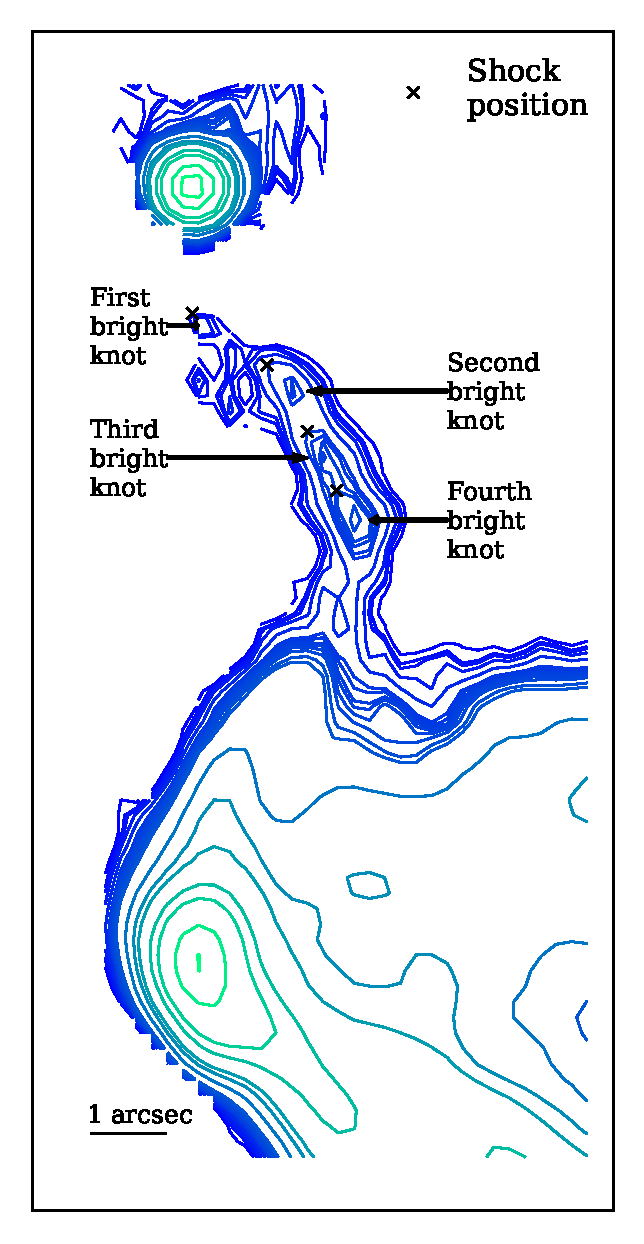
\includegraphics[width=5cm]{southern.eps}
\caption{ Radio intensity map of the central 20~kpc region of the Hydra~A southern jet at 4.635 GHz. Contour levels are at 1.5, 2.0, 2.2, 2.7, 3.7, 5.1, 5.5, 6.0, 6.3, 6.8, 7.5, 8.8, 10, 21, 37, 51,  72, 90, 103, 154, 311, and 466 mJy arcsec$^{-2}$. Four bright knots are marked by arrows. The location of the reconfinement shocks which we interpret as the cause of bright knots are marked by $\times$. }
\label{southern}
\end{figure}

Guided by the models for the northern jet, I  perform a parameter study for the southern jet on the basis of the same proposition that the four bright knots in the southern jet (see Fig.~\ref{taylor}) are the consequence of four consecutive biconical shocks at 2.5, 3.9, 5.4, and 6.7 kpc. As I  discussed earlier, because of the lack of observational data for the radius profile of the jet within 5 kpc from the core, I  only consider the shock positions of this jet.

\subsection{Parametric study for the southern jet}\label{s:param_study}
\begin{figure*}[ht!]
\includegraphics[width=\textwidth]{sps.eps}
\caption{Shock positions, marked by points, for different jet velocity (bottom $x$-axis) and different pressure ratio (top $x$-axis). The horizontal solid lines represent the observed shock locations of the southern jet. The models presented here are deviated from the best fit model for Hydra A northern jet (Ciii, in chapter~\ref{chapter5}), in the jet velocity or, in the over pressure ratio. A visual comparison of the shock locations between the simulations and the observations shows that the best fit model of the southern jet is with $p_{\rm jet}/p_{\rm a}=1$, and $\beta = 0.8$.  }
\label{p_s_s}
\end{figure*}

%The blue dashed lines represent the shock location for the model Ciii of the northern jet. The green solid line represent the observed shock locations of the southern jet. Panel (a) and (b) comprises models deviated from the model Ciii in the jet velocity and the pressure ratio respectively. Panel (c) comprises models with pressure equilibrium jet and with different jet velocities. A visual comparison of the shock locations between the simulations and the observations shows that the best fit model for the southern jet is with $p_\mathrm{jet}/p_\mathrm{a} = 1$, and $\beta = 0.8$.

\begin{figure}[ht!]
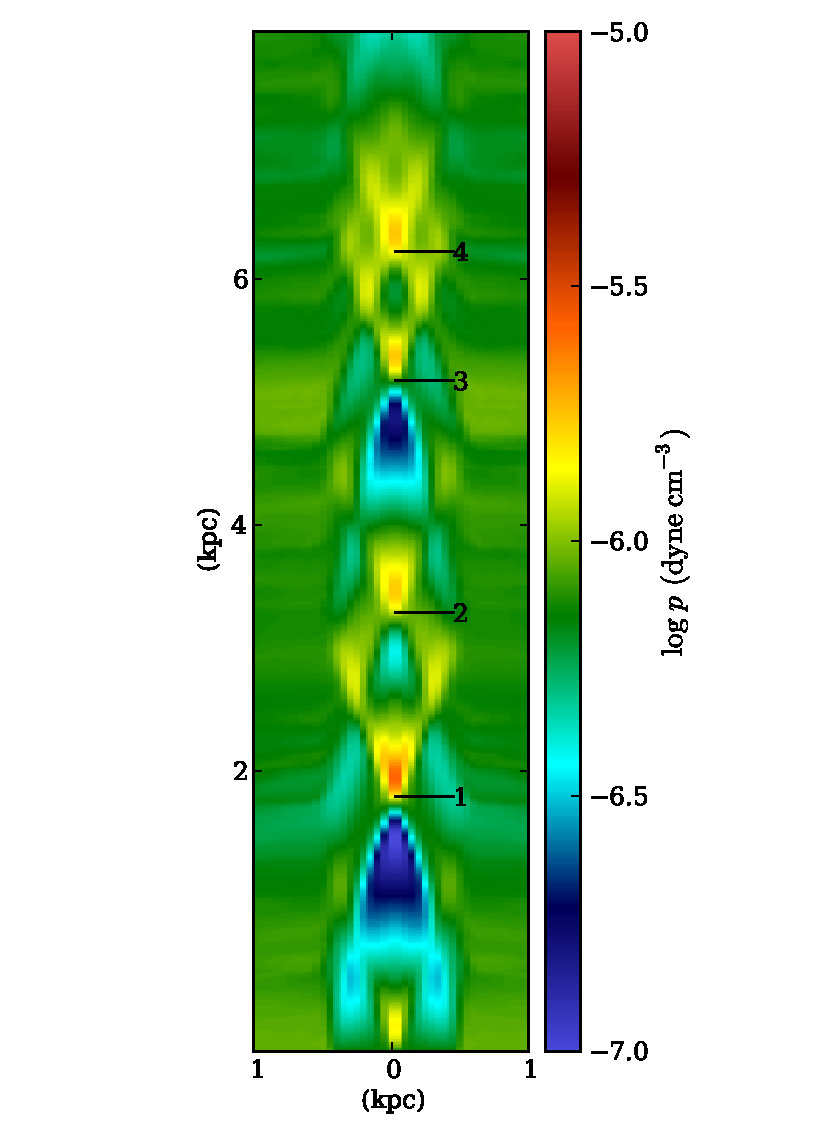
\includegraphics[width=\linewidth]{sbm.eps}
\caption{Logarithmic pressure image of the best fit model for the southern jet (run Dvi) shows the four biconical shocks along the jet marked by 1, 2, 3 and 4.}
\label{m_s_p}
\end{figure}


\begin{table*}
%\begin{sidewaystable}
\caption{Simulation parameters. In all simulations, $P_{\rm{jet}}=10^{45} \rm \ erg \ s^{-1}$.}
\centering
\begin{tabular}{l * {8}{c}}
\hline \hline
Simulation  & $p_{\rm{jet}}/p_{\rm{a}}$ & $\beta$ & $\chi$ & $\eta$ & $\phi$ (rad cm$^{-2}$) & $\Psi_{6\rm{cm}}$ (rad) & $\Psi_{20\rm{cm}}$ (rad) \\
\hline
    %%%%%%%%%% 		set A 	%%%%%%%%%%%%%%%
	\multicolumn{8}{c}{Set E, $r_{\rm{jet}}=0.10 \rm \ kpc$} \\ 
	\hline
  	Ei      & 5    & 0.95 & 0.57    & 3.18$\times10^{-5}$   & 1.61$\times10^{-5}$   & 5.80$\times10^{-4}$   & 6.45$\times10^{-3}$   \\
	Eii     & 5    & 0.96 & 0.15    & 8.33$\times10^{-6}$   & 4.22$\times10^{-6}$   & 1.52$\times10^{-4}$   & 1.69$\times10^{-3}$   \\
	Eiii	& 2   & 0.80 & 35.63    & 7.97$\times10^{-4}$   & 4.04$\times10^{-4}$   & 1.45$\times10^{-2}$   & 1.61$\times10^{-1}$ \\
	Eiv	& 1  & 0.75   & 113.85 & 1.27$\times10^{-3}$   & 6.45$\times10^{-4}$ & 2.32$\times10^{-2}$ & 2.58$\times10^{-1}$ \\
	Ev    & 1  &  0.80  & 73.77   &  8.25$\times10^{-4}$   & 4.18$\times10^{-4}$   & 1.50$\times10^{-2}$   & 1.67$\times10^{-1}$   \\
	Evi      & 1    & 0.85 &  44.66  & 4.99$\times10^{-4}$   & 2.53$\times10^{-4}$   & 9.10$\times10^{-3}$   & 1.01$\times10^{-1}$   \\
		\hline
\end{tabular}
\label{t:sim_par_s}
%\end{sidewaystable}
\end{table*}

We fix the jet power and jet radius to the values of the best-fit model for the northern jet at $P_\mathrm{jet} = 10^{45}$ erg s$^{-1}$ and $r_\mathrm{jet}=100$pc, respectively, and vary only the two other independent jet parameters, the jet velocity and the pressure ratio between the jet and the ambient medium. Because the spacing of the shocks in the southern jet is smaller than that in the northern jet, I explored slightly higher ranges of the jet velocity for a given value of $p_\mathrm{jet}/p_\mathrm{a}$. I  also performed runs with pressure ratios $p_\mathrm{jet}/p_\mathrm{a}=2$ and 1. Simulation parameters for the different models are presented in Table~\ref{t:sim_par_s}.

The parameter $\chi$, which is determined by the other jet parameters through Eqn.~\ref{chi2} becomes negative for jet velocities greater than 0.96, so that this represents the maximum possible jet velocity.  I therefore explored values of  the pressure ratio $p_\mathrm{jet}/p_\mathrm{a} = 2 \rm  \ and \ 1$, keeping the jet velocity fixed at $\beta = 0.8$ (run Eiii, Eiv, Ev, and Evi). The results of different runs are shown in Fig.~\ref{p_s_s}. In this figure the vertical dashed lines represent individual models (labeled by model names) with increasing order from left to right. The overpressure ratio and velocity of each model are presented on the top and bottom axes. The points on each model line represent the shock locations. 

The model with a pressure equilibrium jet and jet (run Ev) produces the required four shocks within the central 7 kpc. To see the dependence of the shock positions on the jet velocity I  ran models with two other jet velocities 0.75 and 0.85. From the comparison of the simulated and observed shock positions I conclude that the best fit model for the southern jet is with jet velocity $\beta = 0.8$. 

Figure~\ref{m_s_p} shows the logarithmic pressure image of the central $2\times8$ kpc domain of the best fit model for the southern jet (run Eiv). This image shows the four consecutive conical shocks marked with 1, 2, 3 and 4.


\section{summary}
\begin{figure*}[ht!]
\includegraphics[width=\textwidth]{sss.eps}
\caption{Logarithmic pressure image for an over-pressured jet (run Ei, left panel) and a pressure equilibrium jet (run Ev, right panel) imposed with the flow velocity. The flow velocity is appears converging at the reflected shock zone in the case of over-pressured jet and to be diverging in the case of pressure equilibrium jet. In the pressure equilibrium case the difference in the expansion rate of the jet in the outer and inner part of the reflected shock zone (marked by the pentangle) cause an extra biconical shock in the reflected shock domain.}
\label{s_s}
\end{figure*}

The axisymmetric models with pressure equilibrium jets produce four bright knots within 8~kpc. This result is consistent with the number of shocks and their locations of the southern jet of Hydra A. A visual comparison of the shock locations between the simulations and the observations shows the the best fit model of the southern jet is with $p_{\rm jet}/p_{\rm a} =1$ and $\beta = 0.8$. Therefore, axisymmetric models of the northern and southern jets based on the knot location (for both cases) and radial oscillation (only for the northern jet) provide a consistent jet velocity for the Hydra A jets. 

I now compare in more detail the flow structure of an over-pressured jet with that of a pressure-equilibrium jet, and describe why in the former case we see two knots and in the latter case four knots. In Fig.~\ref{s_s}, the flow pattern of the over-pressured jet (left panel, run Ei) and the pressure equilibrium jet (right panel, run Ev) overlayed on the pressure image is shown in Fig.~\ref{s_s}. Here we see that an over-pressured jet expands more and the inclination of the incident reconfinement shock is larger than in the case of a pressure equilibrium jet. Hence, In the pressure equilibrium case, the flow is diverging (see right panel of Fig.~\ref{s_s}) at the shocked zone (marked by pentangle). The diverging flow causes rapid expansion, which is counteracted by the formation of another reconfinement shock. Therefore, in the pressure equilibrium case, we have knots in the intermediate spaces of the knot locations of the over-pressured jet and have twice the number of shocks in the pressure equilibrium jet. 

One concern with the modelling of the southern jet is that the observational data is noisy and not well-resolve. It is also possible that the first knot is an observational artefact. Therefore, in the next stage of my study of Hydra A jets with three dimensional models I focus on the northern jet. 



%Therefore when the flow crosses the incident shock it bends more towards the jet axis in the case of over-pressured jet. The flow further changes direction when crossing the reflected shock and in the over-pressured jet the more inclined flow produces a converging zone beyond the reflected shock while in the pressure equilibrium jet we see a diverging zone. Beyond the reflected shock the over-pressured jet expands uniformly and repeat the production of the next biconical shock. However in the pressure equilibrium scenario the jet expands very rapidly within the central part of the reflected shock domain (marked by the white pentangle). The high pressure in the edge of the reflected shock quickly reconfine the inner low pressured jet by an incident shock. Therefore we obtain twice the number of shocks in the pressure equilibrium jet.
\chapter{Complex morphology of the northern jet: An effect of jet precession}\label{chapter7}


Hydra A, located at the centre of the galaxy cluster Abell 780, shows a spectacular S-shaped morphology within the central 20~kpc. The symmetrical S-structure is also visible in the extended low frequency images at 74 and 330~MHz \citep{lane04}. The radio source is extended by approximately 340~kpc in the north and by 190~kpc in the south. Modelling the entire source is computationally impractical and I have adopted the approach of modelling the innermost structures (inner 10~kpc of the northern jet) first in order to constrain jet parameters (see chapter~\ref{chapter5}), then utilising these parameters model the intermediate scale structure (inner 20~kpc of the northern jet). 

I have studied the kinetic power of the Hydra A jets and two key features of the inner 10~kpc of the northern jet: i) the oscillatory jet boundary and ii) two bright knots at approximately 3.7~kpc and 7.0~kpc (see chapters~\ref{chapter3} and \ref{chapter5}). Since the jet is mildly bent within 10~kpc, I have used two dimensional axisymmetric simulations and have modelled the inner two bright knots as biconical reconfinement shocks. By fitting the knot location and the radius profile of the modelled and observed jet I have estimated the jet velocity at 0.5~kpc to be approximately 0.8c, the jet over pressure ratio  with respect to the ICM approximately 5, the jet density parameter approximately 13. 

In this chapter I address the following additional key features of the inner 20~kpc of the northern Hydra A jet: i) the curved jet morphology, ii) two additional bright knots beyond 10 kpc and iii) the turbulent transition of the jet to a dissipative plume. In Fig.~\ref{f:obs} I show the radio structure of the northern jet and indicate these features. This figure is produced using the 4.635~GHz VLA data (G. Taylor, priv. comm.).  The detailed description of these data is available in \citet{taylor90}. In order to model the curved jet morphology I use a three dimensional hydrodynamical model of a precessing jet based on the jet and interstellar medium (ISM) parameters obtained in chapter~\ref{chapter5}. 

%%%%%%%%%%%%%%%%%%%%%%%%%%%%%%%%%%%%%%%%%%%%%%%%%%%%%%%%%%%%%%%%%%%%%%%%
%
%												Details of the model
%
%%%%%%%%%%%%%%%%%%%%%%%%%%%%%%%%%%%%%%%%%%%%%%%%%%%%%%%%%%%%%%%%%%%%%%%%
\section{Details of the model}\label{s:model}
\begin{figure*}
\centering
\includegraphics[width=10cm]{fig1.eps}
\caption{Radio intensity map of the central 20~kpc of the Hydra A northern jet at 4.635 GHz. Contour levels are at 1.5, 2.7, 3.7, 5.1, 6.3, 7.5, 8.8, 10, 21, 37, 51, 72, 90, 103, 150, 180, 200, 205, 220, 240 and 249 mJy arcsec$^{-2}$. Four bright knots are marked with black arrows. The locations of the biconical reconfinement shocks which I interpret as the cause of the bright knots \citep{nawaz14a} are marked with $\times$. An imaginary jet path is traced by a dotted line following the ridge line and joining the four knots. Near the third knot there is a bright knot, marked as 'misaligned knot', which is not aligned with the jet trajectory. The turbulent transition of the jet starts at the location marked by an arrow. The elliptical shaded area outline a dissipative zone.}
\label{f:obs}
\end{figure*}

The motivation for this study is to understand the dynamical interaction of the inner Hydra A northern jet with the interstellar medium and cluster environment and to understand the reason for the source morphology. Therefore, I mainly focus on the features of the inner 20~kpc including i) the curved jet ii) the four bright knots at approximately 3.7~kpc, 7.0~kpc, 11.0~kpc and 16.0~kpc from the core (deprojected) iii) the turbulent transition of the jet to a plume at approximately 10~kpc from the core, and iv) the bright radio emission region at approximately 10 to 20~kpc from the core. 

In chapter~\ref{chapter5} using axisymmetric straight jet simulations I modelled the first two bright knots of the northern jet as biconical reconfinement shocks. Here I develop this model by introducing precession of the jet and this necessitates three dimensional simulations.  According to my model, the jet is initially ballistic and conically expands in the first 0.5~kpc. It then starts to interact with the ISM and is collimated by the ambient pressure. A series of bright knots are produced along the jet path at the locations of the biconical reconfinemnet shocks. 

The initially supersonic jet is decelerated significantly by the first two reconfinement shocks and the jet starts to form a turbulent plume at approximately 11~kpc from the core. The jet strongly interacts with the ISM and produces further reconfinement shocks at approximately 11~kpc and 16~kpc. Some jet plasma is deflected by the dense cocoon wall near the fourth knot and a highly turbulent zone is established in the region approximately 11-20~kpc from the core. 

Note that in the northern Hydra A jet there is a bright knot (marked by 'mis-aligned knot') that is not aligned with the jet path (the black dotted line in Fig.~\ref{f:obs} inferred by following the ridge line and connecting the four bright knots). Prior to conducting the simulations there was no indication as to how this misaligned knot actually formed. 

My modelling strategy is as follows: I conduct a small parameter space study with jet parameters derived from the best fit axisymmetric model of Paper I, a range of precession periods and two values of the precession angle.  I then construct synthetic surface brightness images of the models and compare the source morphology obtained from my models with the observations. Matching the key features, namely, the curvature of the jet, the locations of the bright knots and the turbulent transition of the jet to a plume, I select a best model. 

The input jet parameters, the jet kinetic power $P_{\rm jet} = 1\times 10^{45}$~erg s$^{-1}$, the jet over-pressure ratio $p_{\rm jet}/p_{\rm a} = 5$, the jet velocity $\beta = 0.8$, and the jet density parameter $\chi = 12.75$ are chosen from the best fit axisymmetric model presented in Paper I. I explore a range of values for the precession period $P = 1, 5, 10, 15, 20, 25$~Myr and the precession angle $\theta = 15^{\circ} \rm \ and \ 20^{\circ}$. The grid of models is presented in Table~\ref{t:mod}. Since the radiative cooling timescale of the jet plasma and ambient medium are large compared to the simulation time, I do not include cooling in my models. 

%%%%%%%%%%%%%%%%%%%%%%%%%%%%%%%%%%%%%%%%%%%%%%%%%%%%%
%
%						Numerical Setup
%
%%%%%%%%%%%%%%%%%%%%%%%%%%%%%%%%%%%%%%%%%%%%%%%%%%%%%
\begin{table*}
\centering
\caption{Grid of precessing jet-ICM interaction model. }
%\begin{threeparttable}
\begin{tabular}{*{7}{c}}
\hline \hline
%GVB
% Models &   $P$ & $\theta$  & Computation domain  \\
Model &   Period & Precession   \\
      & (Myr)  & angle (degrees) \\ 
 \\ \hline
   A & 1.0 & 20 \\
   B & 1.0 & 15  \\
   C & 5.0  & 20  \\
   D & 10.0 & 20 \\
   E & 15.0 & 20 \\
   F & 20.0 & 20 \\
   G & 25.0 & 20 \\
\hline
\end{tabular}
\label{t:mod}
%\end{threeparttable}
\end{table*}

%%%%%%%%%%%%%%%%%%%%%%%%%%%%%
%
%			Synthetic surface brightness
%
%%%%%%%%%%%%%%%%%%%%%%%%%%%%%
\subsection{Synthetic surface brightness}
\begin{figure*}
\centering
\includegraphics[width=\textwidth]{fig3.eps}
\caption{Dependencies of the jet morphology on the line of sight and the viewing direction. (a) A cartoon of a spiral jet, an arbitrary line of sight and a viewing cone with cone axis aligned with the jet axis and cone angle equal to the line of sight angle are shown. Any line of sight lying on the viewing cone has the same inclination $\theta$ with the jet axis. The observed source morphology depends on both the line of sight inclination $\theta$ and the viewing direction. (b) The image cube, the data cube and the line of sight (marked by rays) are shown. The data cube is rotated with respect to the image cube to obtain any line of sight and a viewing direction.}
\label{f:con}
\end{figure*}

In order to compare the morphologies derived from the models with the radio observations I produce synthetic surface brightness images for each model. Following \citet{sutherland07}, I use a synchrotron rest-frame emissivity $j_\nu \propto p^{(3+\alpha)/2}$ where  $\alpha$ is the spectral index.  In this expression, the magnetic pressure is assumed to be proportional to the non-thermal particle pressure. The northern Hydra A jet is approaching towards the observer and hence the emissivity $j_\nu$ is modified by the Doppler factor $\delta = 1/\Gamma(1 - \beta \cos\theta]$, where $\Gamma$ is the bulk Lorentz factor and $\theta$ is the angle between the jet axis and the line of sight. In addition, to isolate the jet plasma from the ambient medium I use a tracer $\lambda$, which is the mass concentration of plasma at each cell. I initialise the jet plasma with a value $\lambda = 1$. Hence the emissivity $j_\nu$ becomes (in arbitrary units) 
\begin{equation}
j_\nu = \lambda \delta^{2+\alpha}p^{(3+\alpha)/2}
\end{equation}
Integrating the synchrotron emissivity along rays, parallel to the line of sight, $I_\nu = \int j_\nu ds$, I obtain images of the synthetic surface brightness (in arbitrary units) of the modelled jets. 

I note that the source morphology depends on both the angle between the jet axis and the line of sight and the viewing direction in azimuth. For instance, Fig.~\ref{f:con} shows an arbitrary spiral jet structure about the jet axis and an arbitrary line of sight (making an angle $\theta$ with the jet axis). In this figure a viewing cone is also shown. The axis of the viewing cone lies along the jet axis and its cone angle is equal to the inclination of the line of sight $\theta$. Any line of sight lying on the viewing cone has the same inclination $\theta$ but different azimuthal direction. It is clear from this figure that the jet morphology is different if either $\theta$ or the azimuth direction or both change. Therefore, I scan the synthetic images for different lines of sight and azimuth until I obtain the best match of the synthetic surface brightness to the observations. 

In using the VisIt visualisation software\footnote{https://wci.llnl.gov/simulation/computer-codes/visit/}, it proved to be expedient to work with a fixed image cube and to rotate the computed emissivity cube with respect to this image cube in order to investigate the dependence of the synthetic image on viewing direction. The data cube is rotated so that the line of sight along which the surface brightness is calculated is the $Y$-axis of the image cube. I perform four successive rotations of the data cube ($xyz$) with respect to the image cube ($XYZ$) to obtain a desired line of sight and viewing direction. Details of the transformations are presented in the Appendix~\ref{A:trans}. 

Let $\textbf{v}'$ and $\textbf{v}$ be the velocity vector of the fluid in the image cube and data cube respectively. Then the velocity $\textbf{v}'$ is given by 

\begin{equation}
\textbf{v}' = R \textbf{v}
\end{equation}
where R is the transformation matrix (see Appendix~\ref{A:trans} for the description of $R$).

The angle between the line-of-sight ($Y$-axis) and the fluid velocity at a cell is given by 
\begin{equation}
\theta' = \cos^{-1}v'_Y / v'
\end{equation}
where $v'_Y$ and $v'$ are the $Y$ component and magnitude of the velocity in the image cube, respectively. In order to obtain the correct Doppler factor \emph{for each cell} I use $\theta^{\prime}$ in the expression for the Doppler factor.

Since I am considering the Doppler beaming for individual cell in the simulation data cube, changing the line of sight or viewing direction not only changes the radio morphology of the synthetic image, but the relative brightness of different regions in the source changes as well. In Appendix~\ref{A:morph} I present a collage of surface brightness images of the optimal model (Fig.~\ref{f:morph}) of the Hydra A northern jet for different lines of sight.



%%%%%%%%%%%%%%%%%%%%%%%%%%%%%%%%%%%%%%%%%%%%%%%%%%%%%%%%%%%%%%%%%%%%%%%%
%
%									Simulation Results
%
%%%%%%%%%%%%%%%%%%%%%%%%%%%%%%%%%%%%%%%%%%%%%%%%%%%%%%%%%%%%%%%%%%%%%%%%

\section{Simulation Results}\label{s:results}

In this section I present the results of the three-dimensional precessing jet models. As expected all jets exhibit curvature with the degree of curvature depending upon the precession period and the precession angle. Hence the degree of curvature provides an important diagnostic of the precession parameters, which I discuss below (\S~\ref{curvature}).  I also present other morphological features produced by the various models and compare them with the observations.   
  
\subsection{Curvature of the jet}
\label{curvature}
\begin{figure*}
\centering
\includegraphics[width=\textwidth]{fig4.eps}
\caption{Synthetic surface brightness of models A, B, C, D, E and G. The snapshots are chosen for a simulation time at which the jet is fully developed in the computation domain. }
\label{f:cur}
\end{figure*}

My aim is to match the simulated jet curvature within 10~kpc from the core to the observed curvature of  the Hydra A northern jet. Fig.~\ref{f:cur} shows the synthetic surface brightness images for models A, B, C, D, E, and G. The snapshots are taken when the jet is fully developed in the computational domain.
%aln
Since I am comparing the curvatures of jets with different parameters all images in Fig.~\ref{f:cur} are produced for $\theta = 90^{\circ}$.

In Fig.~\ref{f:cur} it is evident that the curvature of the jet increases as the precession period decreases. Models with longer precession periods produce straight jets within the first 10~kpc. For example, jets produced by the models C, D, E, and G with precession periods 5, 10, 15 and 25~Myr are straight in the inner 10~kpc. The jet with a precession period 1~Myr and a precession angle 15$^{\circ}$ is also nearly straight within this region. We see a mild curvature inside 10~kpc for model A with a precession period 1~Myr and a precession angle 20$^{\circ}$. This curvature is comparable to the curvature of the Hydra A northern jet. Therefore, on the basis of this curvature comparison alone, model A is the best match for Hydra A. This choice is confirmed by other observational features reproduced by the model. In particular, in model~A, no additional knots are produced downstream of the fourth knot. However models with longer precession periods produce more than four bright knots along the jet trajectory. 

\subsection{Bright knots and the turbulent transition of the jet}
\begin{figure*}
\centering
\includegraphics[width=\textwidth]{fig5.eps}
\caption{ A comparison between the source morphology of the best match model (run A, left panel) and the observational data by \citet{taylor90} (middle and right panel).}
\label{f:hyd}
\end{figure*}

\begin{figure*}
\centering
\includegraphics[width=\textwidth]{fig6.eps}
\caption{ Conic slice (cone angle 17$^{\circ}$ and cone axis aligned with the $z$-axis) of the logarithmic density image overlaid with the flow vector of the optimal model (model A) at a simulation time 26 Myr (left panel). The middle panel shows the projection of the cone onto the $x-y$ plane. The right panel is a zoom in image of the region marked by a rectangle in the middle panel.  }
\label{f:fdir}
\end{figure*}

Fig.~\ref{f:hyd} compares the optimal view of the simulated jet of model A (left panel, at a simulation time 22 Myr) and the Hydra A northern jet (middle and right panel). It is evident that the simulated jet successfully reproduces the following key features and processes occurring in the the source within the central 20~kpc. 

The moderately over-pressured precessing jet interacts with the ambient medium and produces four reconfinement shocks at approximately 4.0~kpc, 7~kpc, 10.0~kpc and 14.0~kpc from the core. Since the synchrotron emissivity is $j_{\nu} \propto p^{(3+\alpha)/2}$, downstream of the reconfinement shocks the pressure and therefore the surface brightness increase producing four bright knots. We see that the locations of the bright knots produced with this model agree well with the locations of bright knots in the Hydra A northern jet located at approximately 3.7~kpc, 7.0~kpc, 11.0~kpc and 16.0~kpc (deprojected) from the core and shown in the middle and right panel. In the simulated jet we see that a turbulent transition of the jet to a plume occurs approximately after the second bright knot, which is consistent with the observations.

% This figure also shows that in the optimal model, the turbulent jet starts to forms a dissipative flaring zone (marked by the ellipse in the left panel). This is the beginning of a large plume structure as observed in the Hydra A northern jet.

% Currently, we are investigating further development of the plume for an extended inner region (up to ~30kpc) of the northern jet with high resolution simulations. This will be presented in our next paper.

In the Hydra A northern jet, the flaring region within approximately 11 to 20~kpc from the core where the plume starts, is bright compared to the inner collimated jet. The corresponding region in the optimal model does not reach the same level of brightness. However, the flaring region is strongly turbulent (see \S~\ref{flaring}).
The amplification of the magnetic field resulting from this turbulence may be responsible for the increase in the source brightness. Since, my model is purely hydrodynamic, and the amplification of the magnetic field is not reflected in the synthetic surface brightness images. In order to produce more accurate synthetic brightness images magnetohydrodynamic (MHD) models are required. Therefore, further development of this model with the inclusion of magnetic field is of interest.

\subsection{Turbulent flaring zone}
\label{flaring}
Fig.~\ref{f:fdir} shows the logarithmic density of run A (at a simulation time 26 Myr) sliced by a cone with a cone angle of 17$^{\circ}$ (left panel) and cone axis aligned with the precession axis ($z$ axis). To obtain a clear view of the jet and the flow direction the cone is projected onto the $x-y$~plane (right panel of Fig.~\ref{f:fdir}) and overlaid with the flow vectors. A zoom in of the region marked by a rectangle in the middle panel is shown in the right panel. It is noted here that, although the precession angle in model A is 20$^{\circ}$, the jet is mostly visible along the conic slice with a cone angle 17$^{\circ}$. This is the result of the reflective boundary condition at the lower $z$ boundary. The reflection of the back flow on the side of the jet closest to the boundary pushes the jet towards the precession axis. Therefore, the jet is maximally visible along a conic slice with cone angle less than $20^{\circ}$. 

In Fig.~\ref{f:fdir} we see that after the turbulent transition of the jet some jet plasma hits the relatively dense cocoon plasma and produces a strong back flow (shown in the right panel). This turbulent back flow  establishes a flaring region. Such a flaring region is apparent at approximately 10 to 20~kpc from the core in the northern jet of Hydra A.
 Moreover, in the polarisation image of Hydra A \citep{taylor90} the polarisation significantly falls from 40$\%$ (in the collimated jet) to 10$\%$ in the flaring region. This reduction in polarisation suggests that the flaring region of the northern jet is turbulent and this is consistent with the simulations.  

%%%%%%%%%%%%%%%%%%%%%%%%%%%%%%
%
%			Forward shock
%
%%%%%%%%%%%%%%%%%%%%%%%%%%%%%%
\subsection{Forward shock} 
\begin{figure*}
\centering
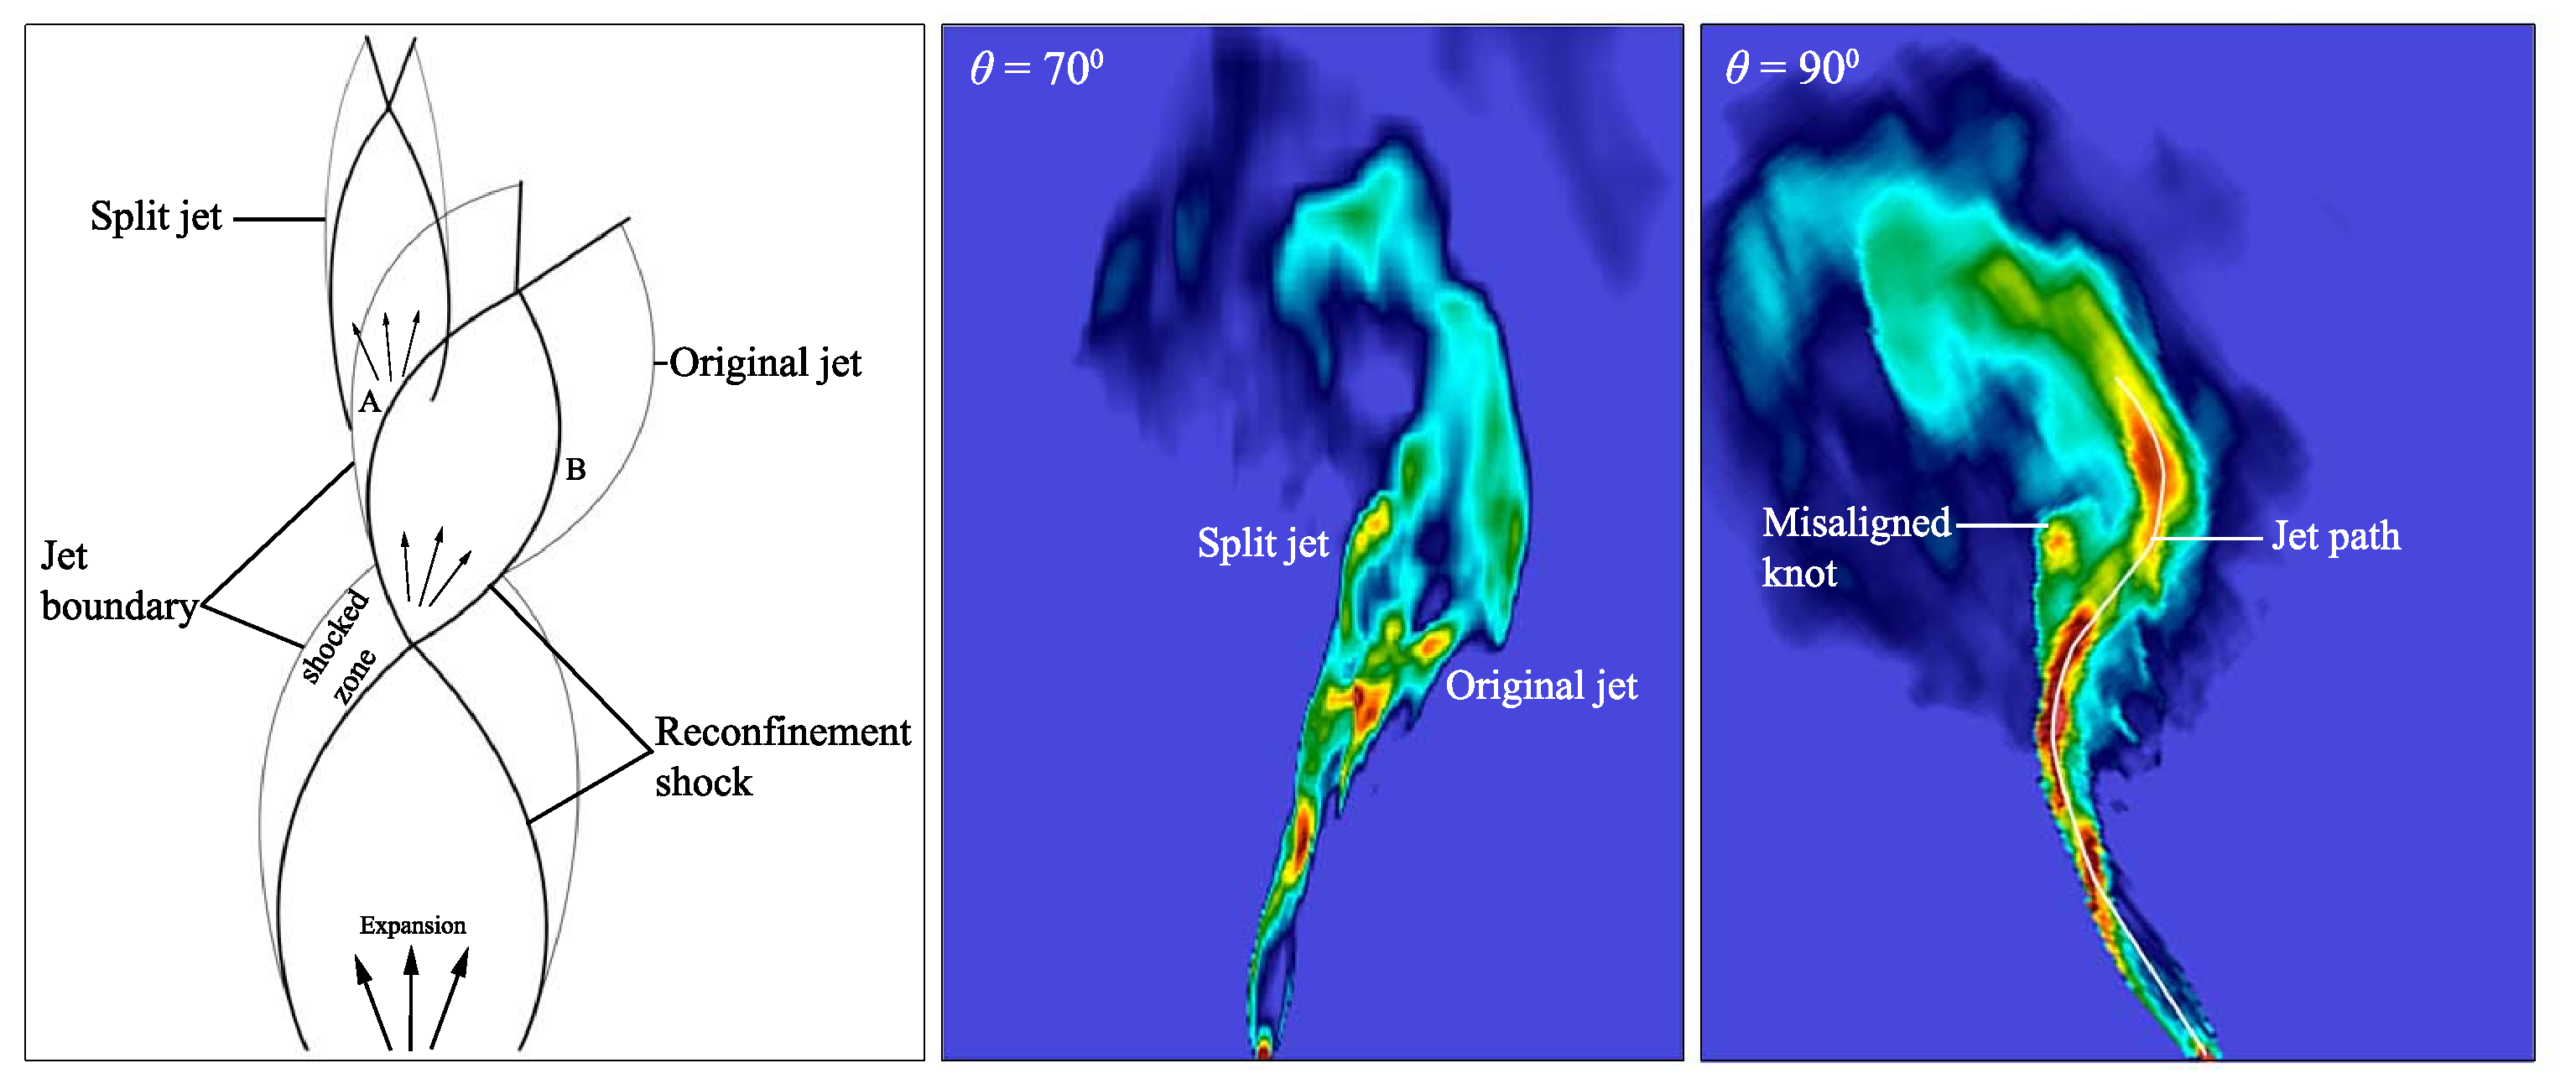
\includegraphics[width=\textwidth]{fig7.eps}
\caption{ Left: Midplane slice of the logarithmic density snapshot of model A. The forward bow shock is marked by an arrow in this panel. Right: Locations of the forward shock at five different time steps (points) . A least square linear fit (line) gives a shock advance speed $\approx$ 1630 km s$^{-1}$. }
\label{f:fsh}
\end{figure*}
%GVB
%In our best natch model the cocoon is separated from the ambient medium by an advancing forward shock. Here we estimate the Mach number of that forward shock. 

In the optimal model the radio jet-ICM interactions are bounded by an advancing forward shock. Here I estimate the Mach number of that forward shock. 

The forward bow shock is shown in the logarithmic density snapshot of model A (left panel of Fig.~\ref{f:fsh}). In the right panel of Fig.~\ref{f:fsh} the location of the forward shock along the $z$-axis at five different time steps is indicated. A least square fit to the shock positions gives a shock advance speed $\approx  1630$ km s$^{-1}$ of the forward shock. The sound speed at approximately 15~kpc from the core is $\approx 880$ km s$^{-1}$. Hence, the Mach number of the forward shock is $\approx 1.85$. 
There is a mild pressure jump $\approx 3.4$ at the forward shock. The low Mach number and mild pressure jump indicate that the heating of the atmosphere by the radio AGN in its earlier stage is gentle. This general feature of the heating of cooling flows was inferred by \citep{mcnamara12}. A straight jet would give a much higher advance speed and a larger pressure jump. The low Mach number and pressure jump derived here can be attributed to the jet precession depositing its momentum over a much wider area. 

%%%%%%%%%%%%%%%%%%%%%%%%%%%%%%
%
%			Mis-aligned knot
%
%%%%%%%%%%%%%%%%%%%%%%%%%%%%%%
\subsection{Misaligned bright knot}
\begin{figure*}
\centering
\includegraphics[width=\textwidth]{fig8.eps}
\caption{A misaligned knot produced by the jet splitting. In the left panel the jet splitting is shown in a synthetic surface brightenss image for a line of sight $\theta = 70^{\circ}$. In the right panel the synthetic surface brightness image is presented for a different line of sight $\theta = 90^{\circ}$, for which the jet path and the misaligned knot are clearly shown. }
\label{f:mknt}
\end{figure*}

In the turbulent flaring region of the Hydra A northern jet there is a  knot, which is not aligned with the main trajectory of the jet. This mis-aligned knot is approximately two kpc north of the third knot and is marked as 'misaligned knot' in Fig.~\ref{f:obs}. This knot is formed as a consequence of the transition to turbulence of the jet. The jet temporarily splits in two forming the misaligned knot and then returns to its final trajectory through the plume region (see Figure~\ref{f:mknt}). This happens only with the optimal model (A).

%Mis-aligned knots appear frequently in synthetic surface brightness images of our best matching model (run A). Models with higher precession periods (run C, D, E, F and G), and model with precession period 1~Myr but low precession angle (run B) do knot produce such mis-aligned knot. The mis-aligned knot usually appear in the flaring region of the jet and are short-lived  compared to the first couple of knots in the main jet at smaller radii. Close inspection of the flow evolution reveals that the jet occasionally splits in two - a main jet and a secondary jet, with the mis-aligned knot forming as a reconfinement shock in the secondary jet. Surveying the surface brightness image evolution of our simulations from a given line of sight, we find that jet splitting and the formation of mis-aligned knots occurs about 2 to 4 times per precession period. It is possible that the occurrence frequency is higher if we included counts along different lines of sights. The splitting of the jet always occurs near the region where the flow transitions to turbulence, and is often in the shape of a tuning fork. We can see that the mis-aligned knot is due to a reconfinement shock because the jet flow remains continuous along the split jet with knots forming at roughly the same distance from the fork. 
%
%The morphology of the split jet with reconfinement shocks forming in both the primary and secondary jet is sketched in panel 1 of Fig.~\ref{f:mknt}. The second and third panels of Fig.~\ref{f:mknt} show a snapshot example from model A (t = 26~Myr) at viewing angles of $\psi=70$ and $\psi=90$ respectively, in which the jet is split and has created two knots, one aligned with the precessional trajectory of the jet, and one clearly offset northward from the main jet. In Appendix~\ref{A:mknt}, we show further examples of the splitting of the jet and the formation of a mis-aligned knot, all at different snapshots from the model A.
%
%The reason for the splitting of the jet is difficult to pin down. Even the exact geometry of the splitting is difficult to reconstruct. We cannot easily determine the orientation of the splitting (i.e., the plane of the ``tuning fork''). Some snapshots of our simulations appear to indicate that the splitting occurs perpendicular to jet along the direction of precession (e.g. panels 2 and 3 Figure ??), In this case, the leading edge of the precessing jet, whose shocked region (region A in panel 1 of Fig.~\ref{f:mknt}) is highly overpressured, is perturbed, allowing the jet to channel, expand, and reconfine in a different direction to the original jet. Due to the incoming flow that compresses the shocked region at the leading edge of the precessing jet, that side is more overpressured than the shocked region of the receding edge (region B in panel 1 of Fig.~\ref{f:mknt}). The leading edge is also more exposed to perturbations as the precessing jet  moves into regions of turbulent backflow. A small blob of slightly denser gas back-flowing into the path of the jet would easily split the jet. This could naturally explain why we often see the split secondary jet emerge from the leading edge of the precessing primary jet. As the primary jet catches up with the split secondary jet, the latter is seen to evolve into the primary jet, while the other jet and its associated knot fades.
%
%The fact that the secondary jet evolves into the primary jet  may also suggests that jet  splitting and the formation of misaligned knots could, in fact, be a manifestation of jet jittering, helical bending of the jet caused by the Kelvin-Helmholtz shear instability \citep{begelman84, hardee13}. The bending would only be temporary because the jet flow keeps re-establishing itself as it precesses to propagate in a different direction. Alternatively, the appearance of knots may simply be related to transition to turbulence giving rise to random bifurcations to the flow direction of the marginally laminar jet. 

%%%%%%%%%%%%%%%%%%%%%%%%%%%%%%%%%%%%%%%%%%
%
%				Implication of precession
%
%%%%%%%%%%%%%%%%%%%%%%%%%%%%%%%%%%%%%%%%%%
\subsection{Implication of precession: Estimate of viscosity parameter of the AGN disk}
Knowledge of the precession period of the jet provides us with information that can be used to estimate the well known accretion disk viscosity parameter $\alpha$. A black hole (BH) whose spin is misaligned with the angular momentum of the accretion disk aligns the surrounding inner part of the disc to the BH spin axis via Lense-Thirring precession and internal viscosity up to a critical radius known as the Bardeen-Petterson radius, $r_\mathrm{BP}$ \citep{bardeen75}. Beyond $r_{\rm BP}$, the disk retains its original structure because of its dominant angular momentum. Viscous torques in the outer accretion disk force the spin axis of the black hole to precess until it is aligned with the angular momentum of the outer disk \citep{rees78, scheuer96, natarajan98, caproni07}. The alignment time-scale can be considered equivalent to the precession period of the jet. Using the alignment timescale, a jet precession period $\approx$ 10$^8$-10$^{10}$ yr has been estimated for the source, NGC 4258 \citep{caproni07}. 

%I use the theory of \citet{natarajan98} to estimate the accretion disk viscosity parameter $\alpha$. 
\citet{natarajan98} estimated the alignment time scale in terms of accretion parameters, including the disk viscosity parameter, $\alpha$. Using their theory, I use the precession period of the optimal model of Hydra A to estimate $\alpha$. 
Let $t_{\rm align}$ be the alignment time-scale, $a$ the spin parameter of the black hole, $\alpha$ the viscosity parameter of the accretion disk, $L$ the total power provided by the black hole,
%($L_{\rm bol}$ + $L_{\rm jet}$), where $L_{\rm bol}$ is the bolometric luminosity of the source, and $L_{\rm jet}$ is the jet kinetic power 
$L_{\rm E}$ the Eddington luminosity, $M_{\rm BH}$ the mass of the black hole, $M_{\odot}$ the solar mass, and $\epsilon$ the accretion efficiency of the black hole. Then, from the equation for the alignment time of the black hole (\citealt[][equation 2.16]{natarajan98}) I obtain:
\begin{align}
\alpha & = 0.04 \left(\frac{a}{0.8}\right)^{-11/26} \left(\frac{L}{0.02 L_{\rm E}}\right)^{7/13} \\ \nonumber 
           & \times \left(\frac{M}{ 10^9 M_{\odot}}\right)^{1/26}  \left(\frac{\epsilon}{0.1}\right)^{-7/13} \left(\frac{P}{\rm Myr}\right)^{8/13}\:.
\end{align}
where $P(=t_\mathrm{align}$) is the precession period of the jet.

The mass of the supermassive black hole in Hydra A is approximately $10^9$ M$_{\odot}$ \citep{fujita13}.
The total jet power provided by the black hole is $L=2L_{\rm jet}\approx 2 \times 10^{45}$ erg s$^{-1}\approx 0.02L_{\rm E}$ and I equate this to the total disk luminosity resulting from accretion. Using $\epsilon = 0.1$, $P=1$~Myr, and a range of $a$ (= 0.1 to 1) I obtain $0.03\le \alpha \le 0.15$. The upper end of the range of $\alpha \approx 0.15$ (for $a \approx 0.1$) is consistent with the range of values typically inferred from observations of dwarf novae $0.1\le \alpha \le 0.4$ \citep{king07}. However, in general, there is a discrepancy between values of $\alpha$ derived from observations and those derived from numerical magneto-hydrodynamic (MHD) simulations; the latter are generally an order of magnitude lower than the former. For instance, the quasi-steady disk MHD models by \citet{parkin13b} imply $\alpha \approx 0.04$. Such a low value is consistent with the lower bound of the estimate of $\alpha$ (for $a\approx 0.9$). The lowest value $\alpha = 0.03$ in the range is consistent with the estimates by \citet{starling04} from observations of AGN disks.


%%%%%%%%%%%%%%%%%%%%%%%%%%%%%%%%%%%%%%%%%
%
%				Appendices
%
%%%%%%%%%%%%%%%%%%%%%%%%%%%%%%%%%%%%%%%%%
\newpage
%\centering{Appendices}
\begin{appendices}
\section{Rotation of the data cube for a desired line of sight}\label{A:trans}
\begin{figure*}
\centering
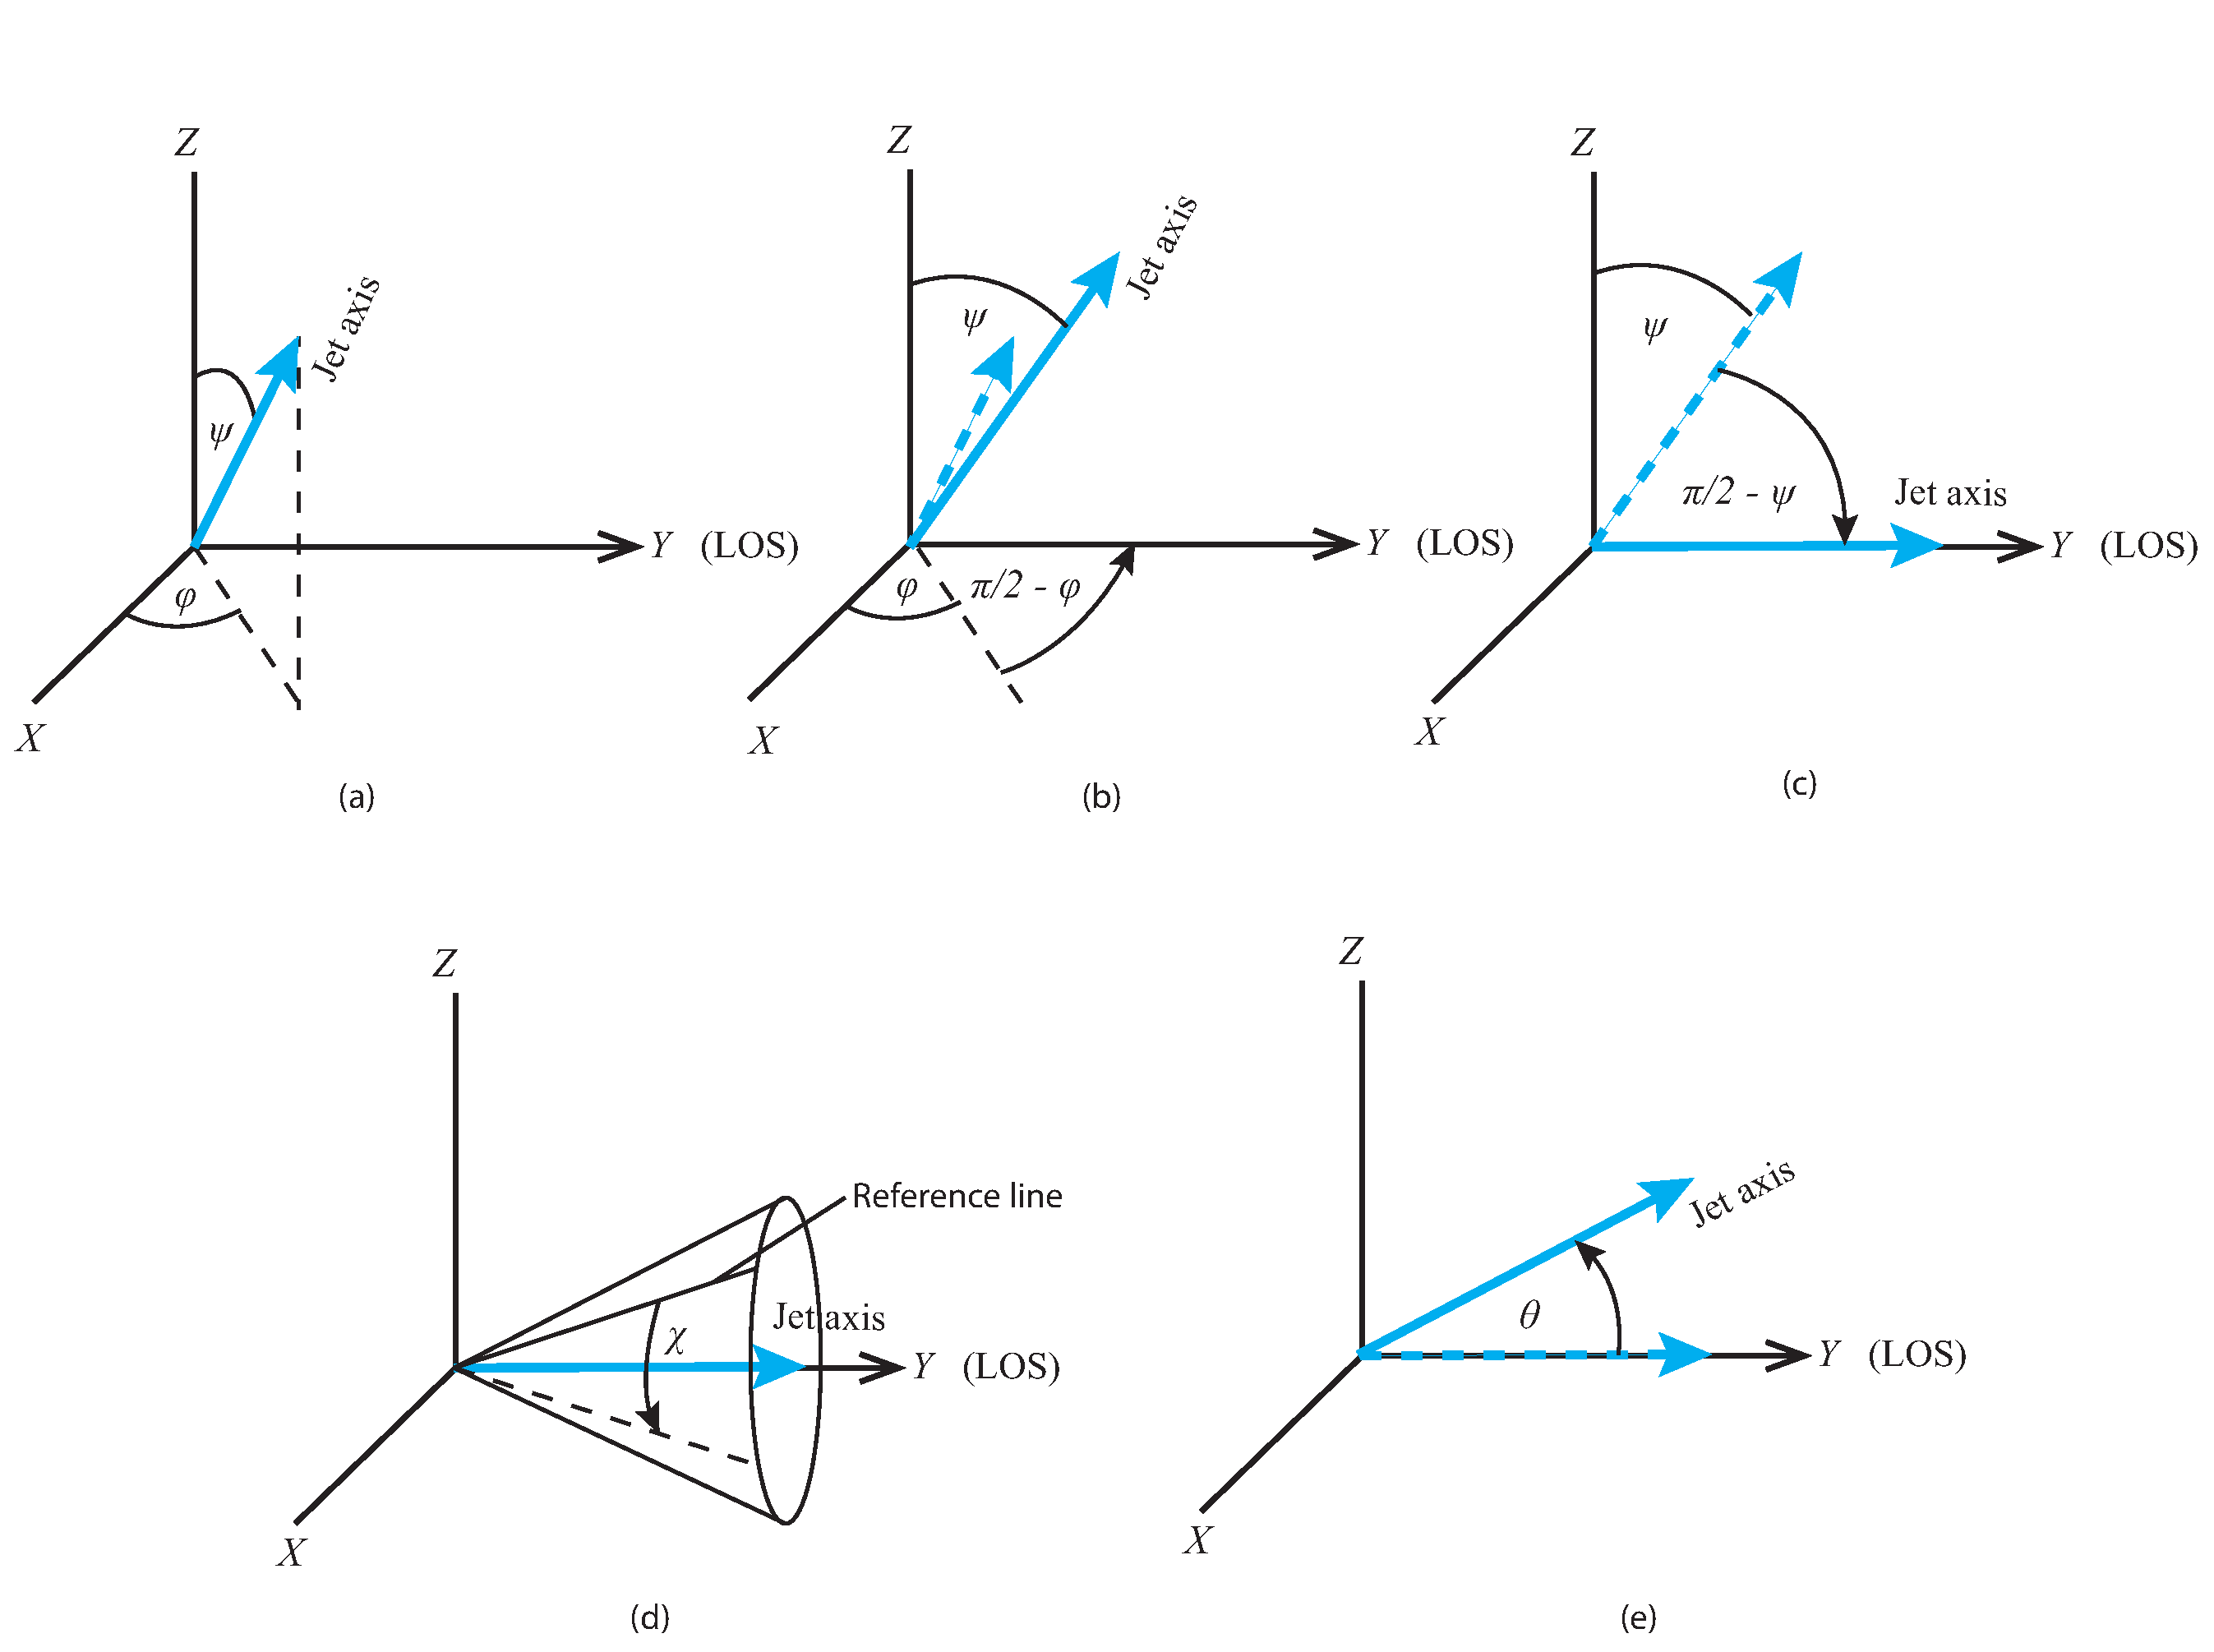
\includegraphics[width=\textwidth]{fig9.eps}
\caption{Transformations associated with the rotations of points of the simulation data cube with respect to the synthetic image cube. Panel (a): At a given instant, both the data cube and the image cube have the same orientation and they can be represented by the same coordinates $XYZ$. Panel (b): Transformation associated with the angle $\phi$, to bring the jet axis on the $YZ$ plane. Panel (c): Transformation associated with the angle $\psi$, to align the jet axis with the line of sight $Y$ axis. Panel (d): Transformation associated with the angle $\chi$, to obtain a desired viewing direction. Panel (e): Transformation associated with the angle $\theta$, to obtain a desired line of sight. In panels (b), (c) and (e) the jet axes before transformations are shown in dashed blue arrows and after transformations with solid blue arrows. In panel (d), the jet does not change its location. It only rotates about its axis. }
%\caption{Transformations of the coordinates associated with the data cube ($xyz$) with respect to coordinates associated with the image cube ($XYZ$) to obtain a line of sight $\theta$ and a viewing direction $\chi$. The line of sight is along the $Y$ axis. See text in Appendix~\ref{A:trans} for details.  }
\label{f:rot}
\end{figure*}
%Let $xyz$ be the coordinates (shown in panel (a) of Fig.~\ref{f:rot}) associated with the simulation data cube. At a given time the jet (shown in a blue thick line in panel (a)) makes angles $\psi$ and $\phi$ with the $z$ and $x$ axes. Let $XYZ$ be the coordinates (shown in panel (a) of Fig.~\ref{f:rot}) associated with the synthetic image cube. 
%To obtain a desired line of sight and viewing direction we perform the following rotations of the simulation data cube with respect to the synthetic image cube. These rotations are depicted in Fig.~\ref{f:rot}. In each panels of this figure the coordinates associated with the image cubes are shown in bold solid lines, the coordinates associated with the simulation data cubes are in solid (before transformations) and dashed (after transformations) lines, the jets before transformations are in light blue thick lines and the jet after transformations are in dark blue thick lines. 
%Transformations of the coordinates associated with the data cube ($xyz$) with respect to coordinates associated with the image cube ($XYZ$) to obtain a line of sight $\theta$ and a viewing direction $\chi$. The line of sight is along the $Y$ axis. See text in Appendix~\ref{A:trans} for details. 

Let $XYZ$ be the coordinates (shown in panel (a) of Fig.~\ref{f:rot}) associated with the synthetic image cube, onto which the ray trace integration is performed. Let $Y$ is the direction of the line of sight. At a given instance the synthetic image cube and the simulation data cube have the same orientation. Hence, at that given instance the direction and location of the jet is defined by the precession angle $\psi$, angle between the jet axis and the precession axis $Z$, and an angle $\phi$ with respect to a fixed axis (say $X$-axis, see panel (a) of Fig.~\ref{f:rot}). Let $\chi$ be the angle defining viewing direction, an angle about the line of sight. To make the angle $
\chi$ understandable, I introduce a viewing cone and a reference line in panel (d) of Fig.~\ref{f:rot}. $\chi$ is then an angle with respect to the reference line. Let $\theta$ be the angle between the jet axis and the line of sight $Y$-axis (see panel (e) of Fig.~\ref{f:rot}).

In order to obtain a desired line of sight $\theta$ and viewing direction $\chi$ I perform the rotations of the data cube with respect to the image cube. In other words, I perform rotations of points (known as \emph{point transformation\footnote{For an anti-clockwise rotation of points by an angle $\theta$ about the origin of a two dimensional coordinate system $XY$, the rotation matrix is given by \begin{eqnarray}
R = \begin{pmatrix}
 \cos\theta & -\sin\theta \\
\sin\theta & \cos\theta \nonumber \\
\end{pmatrix}.
\end{eqnarray}}})
%For a counter-clockwise rotation of a two dimensional coordinate system $XY$ by an angle $\theta$ while the points are fixed, the rotation matrix is given by
%\begin{eqnarray}
%R = \begin{pmatrix}
% \cos\theta & \sin\theta \\
%-\sin\theta & \cos\theta. \nonumber \\
%\end{pmatrix}
%\end{eqnarray}}} ) 
of the data cube with respect to the fixed image cube. 

Since the visualisation software VISIT restricts the choice of the line of sight along any one axis of the image cube (in my case I choose $Y$-axis), we require four rotations; two rotations associated with $\psi$ and $\phi$ to align the jet axis with the line of sight and two rotations associated with $\chi$ and $\theta$ to obtain the desired viewing direction and line of sight. These rotations are depicted in Fig.~\ref{f:rot}. In this figure angles are depicted by arcs and rotations are depicted by arcs with arrowheads. 

%In a point transformation (or, rotation), actual points are rotated with respect to a fixed coordinate system (unlike a nsformation where points are fixed and the coordinates are transformed).  

%Since the choice of the line of sight with the visualisation software VISIT is restricted among any of the axes of the image cube, I choose $Y$ axis as the direction of the line of sight.
%The direction and location of the jet at a given moment is defined by the precession angle $\psi$ and an angle $\phi$ with respect to a fixed axis (say $X$-axis). 
%
%At a given instance the direction and location of the jet (shown by jet axis in each panel) is defined by the precession angle $\psi$ and an angle $\phi$ with respect to an arbitrary axis (say wrt X). 
%
%The choice of the line of sight with the visualisation software VISIT is restricted among any of the axes of the image cube. I choose $Y$ axis as the direction of the line of sight.
%
%Prior to perform any transformation  the synthetic image cube and the simulation data cube have the same orientation. 
%\begin{enumerate}
%\item At a given time the location of the jet is defined by its precession angle $\psi$ and the azimuth angle $\phi$ with respect to $X$ (shown in panel (a)).
%\item  
%\end{enumerate}

% 

%The line of  At a given instance 

%At a given instance the jet (shown in thick blue lines of each panel of Fig.~\ref{f:rot}) makes angles $\psi$ and $\phi$ with the $z$ and $x$ axes. 
%
%At a given time the data cube and the image cube are the same.  In order to obtain a desired viewing direction and line of sight I perform the following rotations of the simulation data cube with respect to the synthetic image cube. 
%
%  At a given time the jet (shown in a blue thick line in panel (a)) makes angles $\psi$ and $\phi$ with the $z$ and $x$ axes. In order to obtain a desired viewing direction and line of sight we require to perform transportation of the data cube with respect to the synthetic image cube.  
%  
%  Let $XYZ$ be the coordinates (shown in panel (a) of Fig.~\ref{f:rot}) associated with the synthetic image cube. 
%To obtain a desired line of sight and viewing direction we perform the following rotations of the simulation data cube with respect to the synthetic image cube. These rotations are depicted in Fig.~\ref{f:rot}. In each panels of this figure the coordinates associated with the image cubes are shown in bold solid lines, the coordinates associated with the simulation data cubes are in solid (before transformations) and dashed (after transformations) lines, the jets before transformations are in light blue thick lines and the jet after transformations are in dark blue thick lines. 
\begin{enumerate}
\item First I rotate the simulation data cube (anticlockwise) with respect to the $Z$-axis by an angle $\pi/2 - \phi$ (shown in panel (b)). %The coordinates associated with the simulation data cube $xyz$ are transformed to $x'y'z'$. 
This rotation brings the jet axis on the $YZ$ plane. The rotation matrix for this rotation $R^{(AC)}_{Z(\pi/2 - \phi)}$ (here the superscript AC denotes the anticlockwise rotation) is given by 
\begin{eqnarray}
R^{(AC)}_{Z(\pi/2 - \phi)}  &=& \begin{pmatrix}
 \cos(\pi/2 - \phi) & -\sin(\pi/2 - \phi) & 0 \\
\sin(\pi/2 - \phi) & \cos(\pi/2 - \phi) & 0 \\
0 & 0 & 1
\end{pmatrix} \nonumber \\
&=& \begin{pmatrix}
 \sin\phi & -\cos\phi & 0 \\
\cos\phi & \sin\phi & 0 \\
0 & 0 & 1
\end{pmatrix} 
\end{eqnarray}
\item I rotate the simulation data cube second time (clockwise) with respect to the $X$-axis by an angle $\pi/2 - \theta$ (shown in panel (c)). 
%The coordinates associated with the simulation data cube $x'y'z'$ are transformed to $x''y''z''$. 
This rotation makes the jet axis aligned with the line of sight $Y$-axis. The rotation matrix for this rotation $R^{(C)}_{X(\pi/2 - \psi)}$ (the superscript C denotes the clockwise rotation) is given by 
\begin{eqnarray}
R^{(C)}_{X(\pi/2 - \psi)} &=& \begin{pmatrix}
 1 & 0 & 0 \\
0 & \cos(\pi/2 - \psi) & \sin(\pi/2 - \psi) \\
0 & -\sin(\pi/2 - \psi) & \cos(\pi/2 - \psi)
\end{pmatrix} \nonumber \\
& = &\begin{pmatrix}
1 & 0 & 0 \\
0 & \sin\psi & \cos\psi \\
0 & -\cos\psi & \sin\psi
\end{pmatrix}  
\end{eqnarray}
\item Now to obtain a viewing direction I rotate the simulation data cube with respect to the $Y$-axis by an angle $\chi$ (shown in panel (d)). 
%The coordinates associated with the simulation data cube $x''y''z''$ are transformed to $x'''y'''z'''$. 
The rotation matrix for this rotation $R^{(AC)}_{Y(\chi)} $ is given by
\begin{equation}
R^{(AC)}_{Y(\chi)} = \begin{pmatrix}
 \cos\chi & 0 & \sin\chi \\
0 & 1  & 0 \\
-\sin\chi & 0 & \cos\chi
\end{pmatrix}  
\end{equation}
\item Finally, I rotate the simulation data cube with respect to the $X$-axis by and angle $\theta$ (shown in panel (e)). This rotation relocates the jet axis at an angle $\theta$ with respect to the $Y$-axis (line of sight). 
%The coordinates associated with the simulation data cube $x'''y'''z'''$ are transformed to $x''''y''''z''''$. 
The rotation matrix associated with this rotation $R'^{(AC)}_{X(\theta)}$ is given by
 \begin{equation}
  R'^{(AC)}_{X(\theta)} = \begin{pmatrix}
 1 & 0 & 0 \\
0 & \cos\theta & -\sin\theta \\
0 & \sin\theta & \cos\theta 
\end{pmatrix}  
\end{equation}
\end{enumerate} 

The velocity of the fluid in the synthetic image cube $\textbf{v}'$ after the transformations described above is estimated from the velocity in the simulation data cube by using the rotation matrix $R = R'^{(AC)}_{X(\theta)} R^{(AC)}_{Y(\chi)} R^{(C)}_{X(\pi/2 - \psi)} R^{(AC)}_{Z(\pi/2 - \phi)}$
\begin{equation}
\textbf{v}' = R \textbf{v}
\end{equation}

Let $s_1 = \sin \psi$, $s_2 = \sin \phi$, $s_3 = \sin \chi$, $s_4 = \sin \theta$, $c_1 = \cos \psi$,  $c_2 = \cos \phi$, $c_3 = \cos \chi$, and $c_4 = \cos\theta$. Then the rotation matrix $R$ is given by:
 \begin{eqnarray}
  R &=&  R'^{(AC)}_{X(\theta)} R^{(AC)}_{Y(\chi)} R^{(C)}_{X(\pi/2 - \psi)} R^{(AC)}_{Z(\pi/2 - \phi)} \nonumber \\
  &=&  \begin{pmatrix}
  c_3 s_2 - s_3 c_1 c_2  & -c_3 c_2 -s_3 c_1 s_2 & s_3 s_1 \\[6pt]
  c_4 s_1 c_2 + s_4 s_3 s_2  &  c_4 s_1 s_2 + s_4 s_3 c_2 & c_4 c_1 - s_4 c_3 s_1  \\
\phantom{{}+{}}+ s_4 c_3 c_1 c_2 & \phantom{{}+{}}- s_4 c_3 c_1 s_2  & & \\[6pt]
   s_4 s_1 c_2 - c_4 s_3 s_2 & s_4 s_1 s_2 + c_4 s_3 c_2  &  s_4 c_1 + c_4 c_3 s_1 \\
\phantom{{}+{}} - c_4 c_3 c_1c_2   &\phantom{{}+{}}-c_4 c_3 c_1 s_2  & & \\
\end{pmatrix} \nonumber 
\end{eqnarray}

% \begin{eqnarray}
%  R &=&  R'^{(AC)}_{X(\theta)} R^{(AC)}_{Y(\chi)} R^{(C)}_{X(\pi/2 - \psi)} R^{(AC)}_{Z(\pi/2 - \phi)} \nonumber \\
%  &=&  \begin{pmatrix}
%  c\chi s\phi - s\chi c\psi c\phi  & -c\chi c\phi -s\chi c\psi s\phi & s\chi s\psi \\[6pt]
%  c\theta s\psi c\phi + s\theta s\chi s\phi  &  c\theta s\psi s\phi + s\theta s\chi c\phi & c\theta c\psi - s\theta c\chi s\psi  \\
%\phantom{{}+{}+{}}+ s\theta c\chi c\psi c\phi & \phantom{{}+{}+{}}- s\theta c\chi c\psi s\phi  & & \\[6pt]
%   s\theta s\psi c\phi - c\theta s\chi s\phi & s\theta s\psi s\phi + c\theta s\chi c\phi  &  s\theta c\psi + c\theta c\chi s\psi \\
%\phantom{{}+{}+{}} - c\theta c\chi c\psi c\phi   &\phantom{{}+{}+{}}-c\theta c\chi c\psi s\phi  & & \\
%\end{pmatrix} \nonumber 
%\end{eqnarray}

%where $s$ and $c$ stands for $\sin$ and $\cos$ respectively. 

% \cos\chi \sin\phi - \sin\chi \cos\psi \cos\phi  & -\cos\chi \cos\phi -\sin\chi \cos\psi \sin\phi & \sin\chi \sin\psi \\

\newpage
\section{Synthetic surface brightness of the source at different $\theta$ and $\chi$}\label{A:morph}
\begin{figure*}
\centering
\includegraphics[width=\linewidth]{fig10.eps}
\caption{ Synthetic surface brightness images of the best match model for different line of sights $\theta$ and viewing directions $\chi$. For comparison the observed radio image of the inner 20~kpc of the Hydra A northern jet is shown at the third column of second row. }
\label{f:morph}
\end{figure*}






\end{appendices}
\chapter{Summary and Discussion}\label{conclusions}
%\doublespacing 

The main aim of this study has been to understand the physics of the inner jets in Hydra~A with a view to inferring parameters such as jet kinetic power, pressure, density and velocity, precession period, precession angle in large scale models of the radio source and its interaction with the cluster atmosphere. I have performed this study in two stages. First, I have studied the inner 10~kpc of the the northern jet, where the jet is nearly straight, using a two dimensional axisymmetric model. Second, I have generalised the axisymmetric model to a three dimensional precessing jet model in order to study the complex morphology of the northern part of the source within 20~kpc from the core. 

\section{Axisymmetric model}
I have focused on the following key features of the radio jet inside 10 kpc from the core i) the bright knots in the northern jet at $\sim 3.7 \rm \ , \ and 7.0$ kpc from the black hole and ii) the wave-like boundary of the northern jet. To this end, I have performed a series of two dimensional axisymmetric relativistic hydrodynamic simulations of the interaction of the northern Hydra A jet with the interstellar medium, particularly within the central $10 \> \rm kpc$. I have utilised the hydrodynamic code PLUTO \citep{mignone07} to perform the 2D axisymmetric models. 

To ensure that I used reasonable values for the jet parameters in my simulations, I have estimated the powers associated with the inner radio lobes of Hydra~A corresponding to inner X-ray cavities. I have used 4.6~GHz radio observations by \citet{taylor90} to estimate the inner cavity power and have compared them with the estimates of \citet{wise07} for the same cavities based on the X-ray data. I obtain powers for the northern and southern cavities $\approx 1.8\times 10^{44} \> \rm ergs \> s^{-1}$ and $2.0\times 10^{44} \> \rm ergs \> s^{-1}$ respectively. These estimates are consistent with the \citet{wise07} estimates $\sim 2 \times 10^{44} \ \rm ergs \ s^{-1}$ for both cavities.
Hence, I adopt the total jet power obtained by \citet{wise07} $P_{\rm jet}=10^{45}$ erg $s^{-1}$ from the summation of powers of all X-ray cavities as the value for the jet power in the numerical models. Other jet parameters, the jet pressure $p_{\rm jet}$ ($= 2 p_{\rm a} \rm \ and \ 5  \ p_{\rm a}$; $p_{\rm a} = $ ambient pressure) and the jet inlet radius $r_{\rm jet}$($=180, 150, \rm \ and \ 100~pc$) are chosen based on the 23~cm VLBA and 6~cm VLA data of Hydra A \citep{taylor90}.

On the basis of minimum pressure estimates I conclude that, in the lobes, $k$, the ratio of energy in other particles to that in relativistic electrons $\sim 10$. Moderate values of this parameter are supported by other recent studies: \citet{birzan08} estimated $k$ for a group of radio galaxies assuming that the radio lobes are in pressure equilibrium with the ambient medium. Their estimates include the Hydra A radio lobes at 1.4 GHz for which they obtained a value of $k \approx 13$. \citet{hardcastle10} studied the inverse-Compton X-ray emission from the outer Hydra A radio lobes and obtained values of $k \sim 17$ and 23 for minimum Lorentz factor cut-offs of $\gamma_1=1$ and 10 respectively. These estimates are all comparable given the different techniques used to derive them. 

For the X-ray atmosphere used in my simulations, I have constructed hydrostatic profiles for the Hydra A atmosphere by fitting and extrapolating the density and temperature data from the X-ray observations of \citet{david01}.

The results of my numerical models of the interaction of an initially conical and ballistic jet with the ambient medium support the idea that consecutive biconical shocks are responsible for the bright knots in the northern jets of Hydra A. With appropriate values of the initial jet pressure ratio and velocity the observed knot spacings and variation in jet radius are reproduced along a considerable section of the jet. 

%I did not model the Southern jet since it is more twisted and a straight jet model would be inappropriate; furthermore the radius of the southern jet as a function of distance from the core has not been observationally determined.

From the comprehensive parameter study in Chapter~\ref{chapter5} I have selected models Ciii, Civ and Cv as are the best fit models for the inner $\sim 10$ kpc radio structure of the northern jet. These jet models with initially conical and ballistic jet, which is over-pressured with respect to the environment by a factor of 5 produce four successive biconical reconfinement shocks before the jets become fully turbulent. The location of the first three shocks and the radius profile of the jet along the direction of its propagation closely match the location of the southern edge of the first three bright knots and the radius profile of the Hydra A northern jet. Constructing a synthetic surface brightness image I have shown that the biconical shocks produced in the simulated jet are associated with bright knots. For the best fit models of the northern jet, the jet parameters are the jet kinetic power $P_{\rm jet}=10^{45} \> \rm erg \rm s^{-1}$,  the jet inlet radius $r_{\rm jet}=100 \rm \> pc$, the jet over pressure ratio  = 5,  the jet density parameter $\chi = 20.41, 12.75, 7.24$ and the jet velocity (in units of the speed of light) $\beta = 0.75, 0.8 \rm \ and \ 0.85$. The estimated jet velocity for the northern jet of Hydra A $\approx 0.8 \rm \> c$ is consistent with recent observational and theoretical estimates of jet velocities in FRI jets determined by \citet{laing14}. In the course of modelling the surface brightness of 10 FRI radio sources they estimated a kpc scale jet velocity $\approx 0.8 \rm \> c$.

The brightnesses of the knots in the best fit model gradually increase with distance from the core, in a way that is qualitatively consistent with the observed jet. However the brightness ratio between the second and first knot and between the third and second knot for the simulated jet (run Ciii) $\approx 2.5$ and 1.14 respectively, differs from the observed brightness ratio $\sim8.7$ and $\sim3$. This discrepancy may arise as a result of the magnetic field increasing faster than the pressure along the jet and hence the assumption of $B^2/8\pi \propto p_{\rm jet}$ in the emissivity model would underestimate the emissivity increase along the jet. 

The inferred relativistic jet velocity $\approx 0.8$~c differs from the estimate based on the Doppler beaming $\approx 0.5$~c. Consequently I estimate a large flux density ratio, 33, of the approaching and receding jet compared to the observed value of 7. The additional parameter study in \S~\ref{s:b_r} shows that the combination $\beta = 0.5$, jet kinetic power $10^{45} \rm \ erg \ s^{-1}$ and an inclination angle $\theta=42^\circ$ is unable to produce the correct shock locations and the profile of the jet boundary for any feasible combination of the jet inlet radius and pressure. Hence, one possibility is to adopt $\beta= 0.8$ and to attribute the different flux density ratio to a difference in intrinsic rest-frame emissivities. For example, the flux density ratio may be overestimated in the best fit model since I assume that the magnetic field is the same in both jets. If I assume that the magnetic field is 2.5 times stronger in the southern jet, the flux density ratio would be 7. Another possibility is that the observed value of the flux density ratio is low since the southern jet is more dissipative as a result of its greater bending and the greater number of shocks. 

Another possibility for the discrepancy between estimated and measured flux density ratios is that the angle, $\theta$, between the jet and the line of sight, inferred from the rotation measure asymmetry \citep[see][]{taylor93} differs from $42^\circ$. This is certainly possible given the range $30^\circ \lesssim \theta \lesssim 60^\circ$  estimated by \citet{taylor93}. Hence, I have used the jet velocity as a parameter, calculated the inclination required to give a northern to southern flux ratio of 7, calculated the deprojected spacing between the first and second knots and compared this with the simulated spacing. The result of this comparison has been that the simulated and observed spacings do not agree except at the lowest possible jet velocities, consistent with a beaming interpretation, $\beta \approx 0.35$. I have argued that a solution for the jet velocity at around $\beta = 0.35$ is unappealing since it is unlikely that the optimal velocity for knot spacing would be fortuitously close to the lower limit from beaming. 
%Moreover, this would imply that the density parameter, $\chi \ga 300$, and this is inconsistent with an electron-positron jet for which there are good arguments based upon X-ray observations and modelling \citep{croston05a,croston14a}. My estimates of $\chi \sim 7 - 20$ for the models based upon an inclination of $42^\circ$ could also be criticised as being inconsistent with an electron-positron jet. However, values of this magnitude could be indicative of some entrainment at this distance form the core.

Taking into consideration the modelling of shock spacing, radius evolution of the jet, and surface brightness ratio, I conclude that the jet velocities $\gtrsim 0.8 \, c$ and that there is an intrinsic asymmetry between the rest-frame emissivities of the northern and southern jets. This may be a result of different magnetic fields (by about a factor of 2.5) or higher dissipation in the southern jet. 


The initial value (at 0.5~kpc) of the density parameter $\chi = \rho c^2 / 4 p$ derived from the simulations is also of interest for the parsec-scale value of this parameter. Assuming that the jet has constant velocity from the pc-scale outwards, $\rho \propto r_{\rm jet}^{-2}$ and $p \propto r_{\rm jet}^{-8/3}$ so that $\chi \propto r_{\rm jet}^{2/3}$. From the VLBI images of \citet{taylor96} $r_{\rm jet} \approx 1 \> \rm pc$ in the 15.4~GHz image. Hence the best fit value of $\chi = 12.75$ extrapolates to 0.59 -- consistent with an electron-positron jet with $\gamma_1 \sim 1$ or an electron proton jet with $\gamma_1 \sim 700$.

 
The conclusions of the axisymmetric models are subject to the assumption of a low magnetic pressure in the jet and I have provided some justification for this assumption, on the sub-parsec scale in \S~3 and the lack of magnetic collimation from the parsec to kiloparsec scale. Nevertheless, the magnetic field evolves along a jet, and its downstream strength and influence on the dynamics is an interesting issue. Moreover, the magnetic field is important for the calculation of synchrotron emission so that even if it passively transported, its evolution is important for the calculation of surface brightness. Hence, the inclusion of a magnetic field in future simulations is of interest. However, as \citet{spruit11a} has shown there is a lot more physics to consider in this case, in particular the modelling of reconnection of three-dimensional magnetic field. Thus, while magnetic effects are important to consider in future work, their consideration is well beyond the scope of this thesis, which I consider to be a useful first step in modelling features such as shock spacing and radial oscillations in order to estimate jet velocities.

\section{Precessing jet model}
With the axisymmetric model I have successfully reproduce the correct oscillations of the jet boundary and the first two bright knots inside 10~kpc of the Hydra A northern jet. In order to study features beyond 10~kpc, where the jet curves significantly, I have generalised the axisymmetric model to a three dimensional precessing jet model. The  three dimensional precessing jet model successfully reproduces the prominent features of the complex inner 20~kpc jet-lobe morphology in the northern side of Hydra A. 

%In Paper I we modelled the inner two bright knots of the Hydra A northern jet utilising axisymmetric straight jet simulations. In this paper we have developed that model by incorporating jet precession and studying the three dimensional interaction of the jet with the intracluster medium. Our three dimensional precessing jet model successfully reproduces the prominent features of the complex inner 20~kpc jet-lobe morphology in the northern side of Hydra A.  

I have performed a parameter space study using parameters obtained from the best fit axisymmetric model, a range of precession periods (1, 5, 10, 15, 20 and 25~Myr) and two precession angles (15$^{\circ}$ and 20$^{\circ}$). From the parameter study presented in chapter~\ref{chapter8} I find that model A with a precession period of 1~Myr and a precession angle of 20$^{\circ}$ produces the correct jet curvature, the correct number of knots, and the jet to plume transition at approximately the correct locations. Therefore I choose this model as the optimal model. 

The optimal model reproduces:
\begin{enumerate}
\item Four bright knots along the direction of the jet. The bright knots appear at the locations of the biconical shocks resulting from reconfinement shocks associated with recollimation of the jet by the ambient medium. The locations of the knots at approximately 4, 7, 10 and 14~kpc coincide reasonably well with the observed bright knots at approximately (3.7, 7.0, 11.0 and 16.0~kpc). 
\item The turbulent transition of the jet to a plume at approximately $9$~kpc compared to the observed transition location at 10~kpc. The initially supersonic jet is significantly decelerated by the first two reconfinement shocks and the transition to turbulence begins after the second knot.  
\item A turbulent flaring zone at approximately 10-20~kpc from the core. The back flowing jet plasma from the cocoon wall near the fourth knot produces strong turbulence in this region. The turbulence is responsible for the widening of the flow at approximately 10~kpc from the core. This simulated feature is consistent with the following observed feature of Hydra A. From the polarisation image \citep{taylor90} we see that the polarisation drops from $40\%$ in the collimated jet (until 10~kpc from the core) to $10\%$ in the flared region (10-20~kpc from the core) on the northern side of Hydra A. This drop in polarisation in this region is consistent with an increase in turbulence there.
\item A misaligned knot in the turbulent flaring zone. This feature is only produced in model A, supporting the choice of that model as the best match to Hydra A. 
\end{enumerate}

%suggests that the flaring zone (10-20~kpc from the core) could be turbulent. 

I have estimated the Mach number of the forward advancing shock $\approx 1.85$ from our optimal model. This low Mach number and the pressure jump ($\approx 3.4$) of the ambient medium associated with the forward shock  suggest a gentle heating of the of the ICM by the radio AGN in its initial phases of evolution as noted by \citet{mcnamara12}. 

Inclusion of magnetic fields in this study would be interesting, mainly for the production of more realistic synthetic surface brightness images. For instance, magnetic field amplification in the turbulent flaring region (10-20~kpc) of the northern jet may be a possible explanation for the increase in brightness there. However, a purely hydrodynamic model does not capture this effect. For this reason, in our optimal model, the ratio of the brightness between the initial jet (up to 10~kpc from the core) and the turbulent plume (10-20~kpc from the core) is not reproduced correctly. 

In the models presented here I have only considered the inner 20~kpc morphology of the northern jet. Since the initial jet radius (0.1~kpc) is very small compared to the extent of the inner lobe (50~kpc), modelling the entire inner lobe for a large range of parameters is unrealistic. However the parameters I have obtained by modelling the inner 20~kpc northern jet morphology can be used as input into future large scale studies of this source. 

On the southern side the initial 5~kpc trajectory of the jet is not well determined observationally. Therefore, adequate modelling of the southern side of the source as I have done for the northern side requires further high resolution observations of the source. 

Interpreting the realignment time-scale estimate by \citet{natarajan98} as the precession period of the jet, I have estimated the viscosity parameter of the accretion disk of Hydra A to be $0.03\le \alpha \le 0.15$. 
The lower values of $\alpha$ within this range are consistent with the prediction from quasi-steady MHD disk models \citep{parkin13b}. 
\chapter{Future Work}\label{future_work}
%\doublespacing
The study of Hydra A inner 10~kpc jet presented in this thesis uses an innovative method for the estimation of jet velocity by combining the information of the inner knot locations and the oscillation of the the jet boundary.

The detailed parameter study presented in this thesis using this technique provides best fit jet parameters, which can be used for a even more realistic three dimensional modelling of the dynamical interaction of the Hydra A jets and the cluster atmosphere.

In the following I describe the studies that could be done in future guided by the methodology I have used and the results we obtained in this thesis.

%\section{The turbulent transition of Hydra A jets}
%As I discussed in chapter~\ref{chap4} the turbulent transition of a jet is a three dimensional phenomenon, which cannot be captured well with the two dimensional axis-symmetric jet models. The turbulent transition of the jet originates from the shear layer at the jet boundary. This shear layer is Kelvin-Helmholtz unstable. The instability grows very rapidly and causes the jet to become turbulent in the region where the jet becomes subsonic due to the reconfinement shock deceleration. Beyond this point, and either side of the shear layer the flow is turbulent. In this context it is important to remember that two-dimensional turbulence behaves differently to three-dimensional turbulence: enstrophy (the square of the vorticity) is conserved in two-dimensional turbulence but not conserved in three-dimensional turbulence, and energy cascades in two-dimensional turbulence do not show the same scaling universality down to small scales as in three dimensions. The turbulent transition may therefore not be correctly captured in two-dimensional axis-symemtric simulations.
%
%One direct consequence of enstrophy conservation seen in my 2-D simulations is the perturbation of the jet boundary by the back-flowing plasma vortices that travel towards the computational symmetry axis. The ram pressure of the vortices pushes the jet boundary toward the symmetry axis and when the jet boundary layer reaches the symmetry axis the jet stream temporarily disappears until new jet plasma reaches the affected zones to reestablish the jet stream. This phenomenon is sometimes referred to as jet pinching and it affects the growth of instabilities in the shear layer. Jet pinching is an unavoidable numerical artifact associated with the axisymmetric jet model. Sufficiently resolved three dimensional jets are rarely pinched and their additional degree of freedom allows for axis-symmetry to be broken. Instead, a different physical instability is often observed, namely that of jet jittering. Jet jittering may itself increase the deceleration rate and, therefore, a more realistic three dimensional jet model is required to study the turbulent transition of the Hydra A jets.
% 
%In the case of the Hydra A northern jet, one may directly use the jet parameters obtained through the parameteric study to initialize models of three dimensional jet-ICM interaction and study the turbulent transitions of the jets.

\section{The large scale morphology of the Hydra A}
In this thesis I have modelled the inner 20~kpc structures of the Hydra A northern jet, including the width profile of the jet, the bright knots along its axis, the curvature of the jet and the jet to plume transition. This is a good starting point for a bottom up approach to study different scales of a very extended source like Hydra A. Following the evolution of the jet plasma, one could first investigate the inner 50~kpc radio plume, then the series of X-ray cavities, and finally attempt to explain the large scale structures in the X-ray images including the outer shock at approximately 200~kpc. Energy and mass transport measurements from three-dimensional simulations, in particular the transport of metal rich gas from the galaxy center, across these scales will provide answers to how cooling flows are suppressed, and allow direct comparisons with ICM temperature and metal distribution maps, and observations of cold filaments.

%In this thesis I have modelled the inner 20~kpc structures of the Hydra A northern jet, including the width profile of the jet, the bright knots along its axis, the curvature of the jet and the jet to plume transition. This is a good starting point for a bottom up approach to study different scales of a very extended source like Hydra A. Following the evolution of the jet plasma, one could first investigate the medium-scale structures such as the turbulent transition of the jet to a plume and the high dissipative zones described above, followed by the inner 50~kpc radio plume, then the series of X-ray cavities, and finally attempt to explain the large scale structures in the X-ray images including the outer shock at approximately 200~kpc. Energy and mass transport measurements from three-dimensional simulations, in particular the transport of metals from the galaxy center, across these scales will provide answers to how cooling flows are suppressed, and allow direct comparisons with ICM temperature and metal distribution maps, and observations of cold filaments.

\section{Magnetohydrodynamic models} 
In this thesis I use a pseudo synthetic emissivity as a function of pressure derived by \citep{sutherland07} to obtain the synthetic surface brightness image of the modelled jet. However, a proper calculation of synchrotron emission requires magnetic field. Therefore, a realistic study of the radio jets and the lobes requires magnetohydrodynamic (MHD) modelling of the source. One can incorporate magnetic filed into the purely hydrodynamic model I developed in this work and study the radio features in an even more realistic way.

%\section{A precessing jet model for Hydra A}
%In the models for the northern jet of Hydra A presented here, I used a straight jet assumption which is reasonable because the northern jet is only mildly bent. However, a more realistic three-dimensional model is also required in order to interpret the jet curvature. A precessing jet model could produce the observed bending. It is possible to model a three dimensional precessing jet with the parameters obtained in this thesis. Such a precessing jet model could be used to investigate the 10-30~kpc region of the northern plume region, for example, i) the bent jet structure, ii) two additional brighter knots in the northern jet beyond 10~kpc, and iii) the highly dissipative zone at 10-20~kpc. The precessing jet model is also important to study the impact of precession on the jet morphology on scales from 30 kpc to 200 kpc and the energy and material transport from the central black hole to the outer cluster atmosphere.

\section{The modelling of AGN jets displaying inner knots}
In this thesis, I showed that simultaneously modelling the data on the locations of the inner knots and the oscillation of the boundary of the Hydra A northern jet can be used to estimate the velocity of the jet. This method of estimation of the jet velocity can in principle be applied with modifications to other radio

\section{Modelling complex morphologies of other radio sources}
\begin{figure}
\centering
\includegraphics[width=\linewidth]{cenA.jpg}
\caption{ A comparison between the simulated source morphology (left panel) for model G ( precession period $P = 25$~Myr) and the radio morphology of Centurus A (inset of the right panel). Credit for the Centaurus A image: CSIRO.}
\label{f:cenA}
\end{figure}
\begin{figure}
\centering
\includegraphics[width=\linewidth]{m87.jpg}
\caption{ A comparison between the simulated source morphology (left panel) for model G ( precession period $P = 25$~Myr) and the radio morphology of m87 (inset of the right panel). Credit for the m87 image: NRAO. }
\label{f:m87}
\end{figure}
%Credit for the m87 image: NRAO.

In my precessing jet models I notice a generic morphological feature of the precessing jet. In the first half cycle of the jet precession, we see a jet structure leading a balloon shaped lobe behind it. This type of jet-lobe morphology is common in some sources, for example, Centaurus A, M87 (inner lobe), J0116-473 etc.

 Fig.~\ref{f:cenA} and \ref{f:m87} shows the morphological similarities between the simulated radio image of the source (in the left panels) for model G (precession period $P = 25$~Myr) and the observed radio morphology of Centaurus A and M87 (in the right panels). The snapshots are captured when the jet reaches approximately half (Fig.~\ref{f:cenA}) and approximately quarter (Fig.~\ref{f:m87}) of its precession cycle. Therefore, modelling precessing jet can be a potential strategy to study sources with this type of jet-lobe morphology.  

\section{Maintenance mode feedback}
Precessing jet model also has the potential to interpret the maintenance mode feedback (balance of the heating and cooling for long duration). In case of a straight jet, most of the jet energy deposits well outside of the core. Hence, for a straight jet it is difficult to prevent a catastrophic cooling flow \citep{vernaleo06}. However, a precessing jet with a low precession period always strongly interact with the environment near the core. For example, in the optimal model for the Hydra A northern jet ( precession period = 1~Myr, run A of chapter~\ref{chapter8}), the jet maintains a turbulent dissipative zone at approximately 10~kpc to 20~kpc from the core (the extent of the source is approximately 340~kpc in the north). Hence, a long term balance between the heating and cooling (maintenance mode feedback) is possible by a precessing jet model. Incorporating cooling in the precessing jet model presented here one can study the maintenance mode feedback by AGN sources. 










%\chapter{Appendix material}

\section{Coordinate transformation for a desired line of sight and viewing direction}\label{A:trans}
\begin{figure*}
\centering
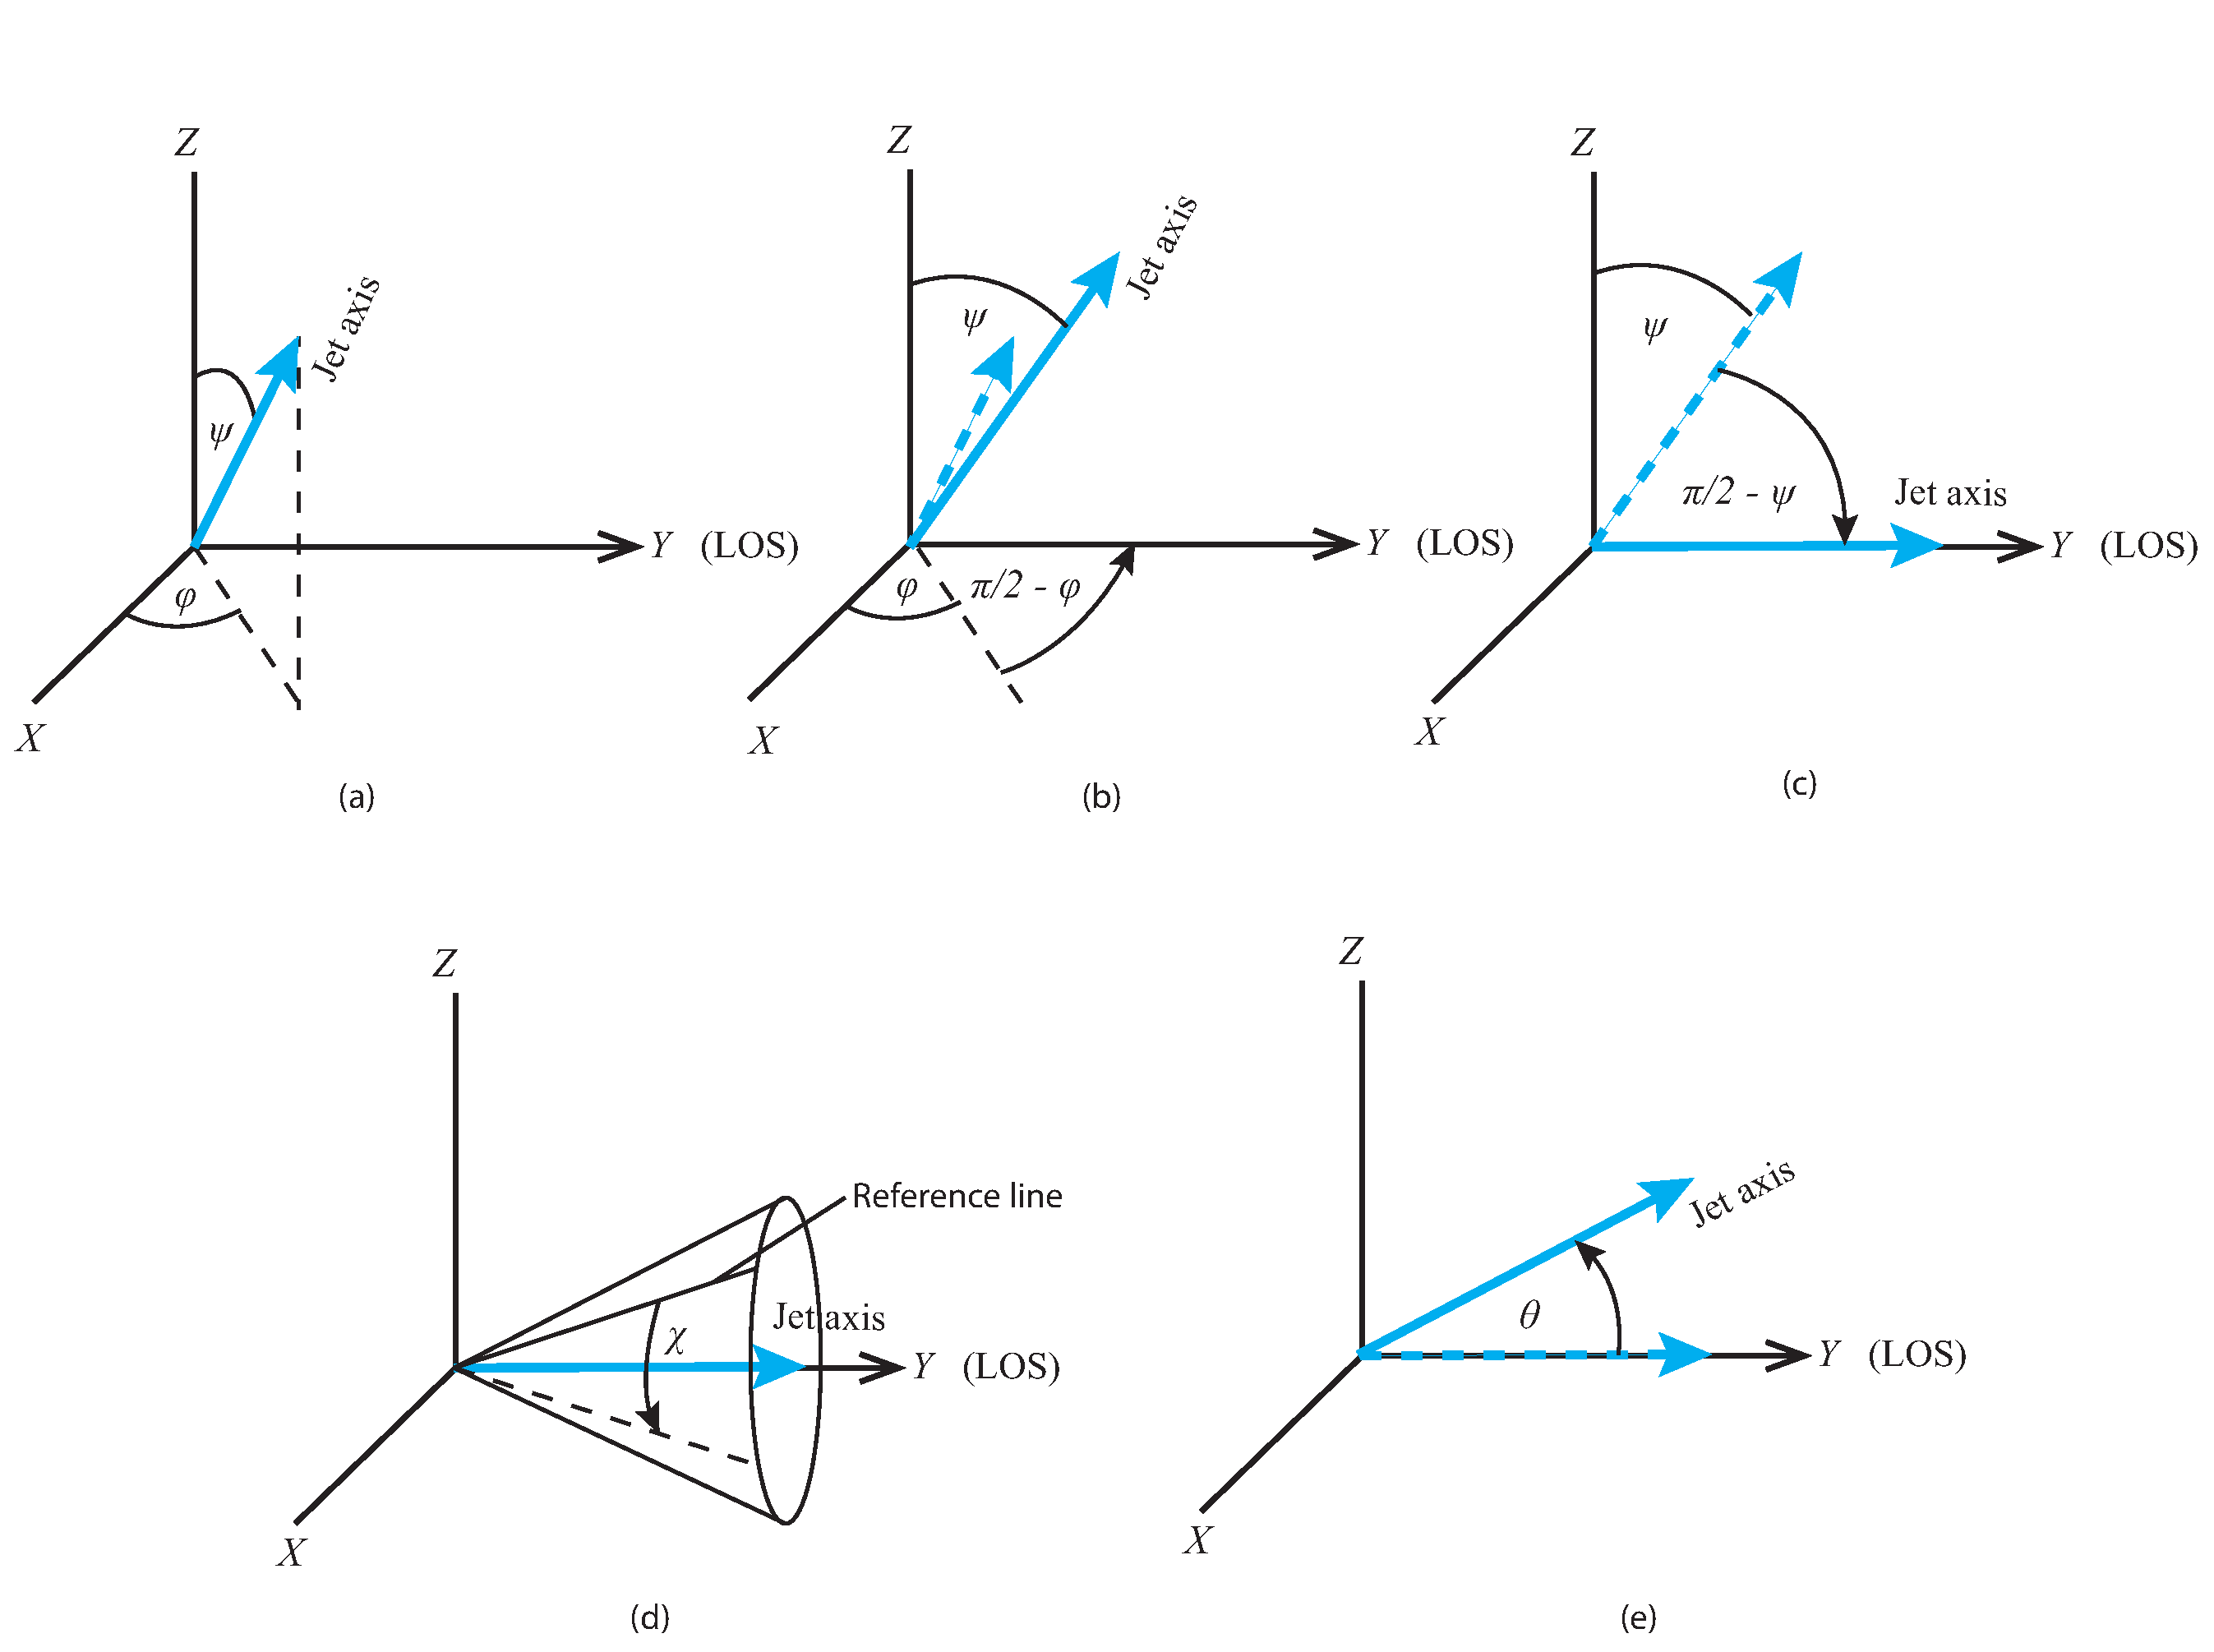
\includegraphics[width=\textwidth]{fig9.eps}
\caption{Transformations of the coordinates associated with the data cube ($xyz$) with respect to coordinates associated with the image cube ($XYZ$) to obtain a line of sight $\theta$ and a viewing direction $\chi$. The line of sight is along the $Y$ axis. See text in Appendix~\ref{A:trans} for details.  }
\label{f:rot}
\end{figure*}
Let $xyz$ be the coordinates (shown in panel (a) of Fig.~\ref{f:rot}) associated with the simulation data cube. At a given time the jet (shown in a blue thick line in panel (a)) makes angles $\psi$ and $\phi$ with the $z$ and $x$ axes. Let $XYZ$ be the coordinates (shown in panel (a) of Fig.~\ref{f:rot}) associated with the synthetic image cube. 
To obtain a desired line of sight and viewing direction we perform the following rotations of the simulation data cube with respect to the synthetic image cube. These rotations are depicted in Fig.~\ref{f:rot}. In each panels of this figure the coordinates associated with the image cubes are shown in bold solid lines, the coordinates associated with the simulation data cubes are in solid (before transformations) and dashed (after transformations) lines, the jets before transformations are in light blue thick lines and the jet after transformations are in dark blue thick lines. 
\begin{enumerate}
\item First we rotate the simulation data cube (anticlockwise) with respect to the $Z$-axis by an angle $\pi/2 - \phi$ (shown in (a)). The coordinates associated with the simulation data cube $xyz$ are transformed to $x'y'z'$. This rotation brings the jet on the $YZ$ plane. The rotation matrix for this rotation $R^{(AC)}_{Z(\pi/2 - \phi)}$ (here the superscript AC denotes the anticlockwise rotation) is given by 
\begin{eqnarray}
R^{(AC)}_{Z(\pi/2 - \phi)}  &=& \begin{pmatrix}
 \cos(\pi/2 - \phi) & -\sin(\pi/2 - \phi) & 0 \\
\sin(\pi/2 - \phi) & \cos(\pi/2 - \phi) & 0 \\
0 & 0 & 1
\end{pmatrix} \nonumber \\
&=& \begin{pmatrix}
 \sin\phi & -\cos\phi & 0 \\
\cos\phi & \sin\phi & 0 \\
0 & 0 & 1
\end{pmatrix} 
\end{eqnarray}
\item We rotate the simulation data cube second time (clockwise) with respect to the $X$-axis by an angle $\pi/2 - \theta$ (shown in panel (b)). The coordinates associated with the simulation data cube $x'y'z'$ are transformed to $x''y''z''$. This rotation makes the jet axis aligned with the line of sight $Y$-axis. The rotation matrix for this rotation $R^{(C)}_{X(\pi/2 - \psi)}$ (the superscript C denotes the clockwise rotation) is given by 
\begin{eqnarray}
R^{(C)}_{X(\pi/2 - \psi)} &=& \begin{pmatrix}
 1 & 0 & 0 \\
0 & \cos(\pi/2 - \psi) & \sin(\pi/2 - \psi) \\
0 & -\sin(\pi/2 - \psi) & \cos(\pi/2 - \psi)
\end{pmatrix} \nonumber \\
& = &\begin{pmatrix}
1 & 0 & 0 \\
0 & \sin\psi & \cos\psi \\
0 & -\cos\psi & \sin\psi
\end{pmatrix}  
\end{eqnarray}
\item Now to obtain a viewing direction we rotate the simulation data cube with respect to the $Y$-axis by an angle $\chi$ (shown in panel (c)). The coordinates associated with the simulation data cube $x''y''z''$ are transformed to $x'''y'''z'''$. The rotation matrix for this rotation $R^{(AC)}_{Y(\chi)} $ is given by
\begin{equation}
R^{(AC)}_{Y(\chi)} = \begin{pmatrix}
 \cos\chi & 0 & \sin\chi \\
0 & 1  & 0 \\
-\sin\chi & 0 & \cos\chi
\end{pmatrix}  
\end{equation}
\item Finally, we rotate the simulation data cube with respect to the $X$-axis by and angle $\theta$ (shown in panel (d)). This rotation relocates the jet (shown in dark blue thick line) at an angle $\theta$ with respect to the $Y$-axis (line of sight). The coordinates associated with the simulation data cube $x'''y'''z'''$ are transformed to $x''''y''''z''''$. The rotation matrix associated with this rotation $R'^{(AC)}_{X(\theta)}$ is given by
 \begin{equation}
  R'^{(AC)}_{X(\theta)} = \begin{pmatrix}
 1 & 0 & 0 \\
0 & \cos\theta & -\sin\theta \\
0 & \sin\theta & \cos\theta 
\end{pmatrix}  
\end{equation}
\end{enumerate} 

The velocity of the fluid in the synthetic image cube $\textbf{v}'$ after the transformations described above is estimated from the velocity in the simulation data cube by using the rotation matrix $R = R'^{(AC)}_{X(\theta)} R^{(AC)}_{Y(\chi)} R^{(C)}_{X(\pi/2 - \psi)} R^{(AC)}_{Z(\pi/2 - \phi)}$
\begin{equation}
\textbf{v}' = R \textbf{v}
\end{equation}

Let $s_1 = \sin \psi$, $s_2 = \sin \phi$, $s_3 = \sin \chi$, $s_4 = \sin \theta$, $c_1 = \cos \psi$,  $c_2 = \cos \phi$, $c_3 = \cos \chi$, and $c_4 = \cos\theta$. Then the rotation matrix $R$ is given by:
 \begin{eqnarray}
  R &=&  R'^{(AC)}_{X(\theta)} R^{(AC)}_{Y(\chi)} R^{(C)}_{X(\pi/2 - \psi)} R^{(AC)}_{Z(\pi/2 - \phi)} \nonumber \\
  &=&  \begin{pmatrix}
  c_3 s_2 - s_3 c_1 c_2  & -c_3 c_2 -s_3 c_1 s_2 & s_3 s_1 \\[6pt]
  c_4 s_1 c_2 + s_4 s_3 s_2  &  c_4 s_1 s_2 + s_4 s_3 c_2 & c_4 c_1 - s_4 c_3 s_1  \\
\phantom{{}+{}}+ s_4 c_3 c_1 c_2 & \phantom{{}+{}}- s_4 c_3 c_1 s_2  & & \\[6pt]
   s_4 s_1 c_2 - c_4 s_3 s_2 & s_4 s_1 s_2 + c_4 s_3 c_2  &  s_4 c_1 + c_4 c_3 s_1 \\
\phantom{{}+{}} - c_4 c_3 c_1c_2   &\phantom{{}+{}}-c_4 c_3 c_1 s_2  & & \\
\end{pmatrix} \nonumber 
\end{eqnarray}

% \begin{eqnarray}
%  R &=&  R'^{(AC)}_{X(\theta)} R^{(AC)}_{Y(\chi)} R^{(C)}_{X(\pi/2 - \psi)} R^{(AC)}_{Z(\pi/2 - \phi)} \nonumber \\
%  &=&  \begin{pmatrix}
%  c\chi s\phi - s\chi c\psi c\phi  & -c\chi c\phi -s\chi c\psi s\phi & s\chi s\psi \\[6pt]
%  c\theta s\psi c\phi + s\theta s\chi s\phi  &  c\theta s\psi s\phi + s\theta s\chi c\phi & c\theta c\psi - s\theta c\chi s\psi  \\
%\phantom{{}+{}+{}}+ s\theta c\chi c\psi c\phi & \phantom{{}+{}+{}}- s\theta c\chi c\psi s\phi  & & \\[6pt]
%   s\theta s\psi c\phi - c\theta s\chi s\phi & s\theta s\psi s\phi + c\theta s\chi c\phi  &  s\theta c\psi + c\theta c\chi s\psi \\
%\phantom{{}+{}+{}} - c\theta c\chi c\psi c\phi   &\phantom{{}+{}+{}}-c\theta c\chi c\psi s\phi  & & \\
%\end{pmatrix} \nonumber 
%\end{eqnarray}

%where $s$ and $c$ stands for $\sin$ and $\cos$ respectively. 

% \cos\chi \sin\phi - \sin\chi \cos\psi \cos\phi  & -\cos\chi \cos\phi -\sin\chi \cos\psi \sin\phi & \sin\chi \sin\psi \\

\section{Synthetic surface brightness of the source at different $\theta$ and $\chi$}\label{A:morph}
\begin{figure*}
\centering
\includegraphics[width=\textwidth]{fig10.eps}
\caption{ Synthetic surface brightness images of the best match model for different line of sights $\theta$ and viewing directions $\chi$. For comparison the observed radio image of the inner 20~kpc of the Hydra A northern jet is shown at the third column of second row. }
\label{f:morph}
\end{figure*}






































%\section{Table~\ref{table:Sayurirrab}}
%

%A cross-match between the current data set and that of \citet{prior09} confirmed four objects as RRab. Of these, two were previously identified as undefined variables, one as non-variable and the other one as RRc. Object 116385.432 was identified as RRab by \citet{prior09}. We find this star as a Blazhko RRab as we have two sets of observations separated by $\sim100$ days. These are given in Table~\ref{table:Sayurirrab}. While calculating the completeness profiles, these objects were considered as RRab (Sections~\ref{s3.3} and ~\ref{s5}).
%
%\section{Table~\ref{table:fromSayuri}}
%
%This table presents two objects that were confirmed as RRLs by \citet{prior09}, but could not be identified in this study due to insufficient observations. A third object 115213.329 is clarified as RRab with the help of \citet{prior09}'s catalog. We found the same period. However, we could not confirm the amplitude as we need more observations. We considered these three objects as RRLs in the completeness profile calculations, though we could not calibrate them photometrically.
%
%\ctable[sideways,cap=Objects Reidentified by Current Study from \citet{prior09},caption=Objects Reidentified by Current Study from \citet{prior09},label=table:Sayurirrab,doinside=\normalsize \setlength{\extrarowheight}{2pt}
%,captionskip=3pt]{lccccccccccc}
%{\tnote[a]{Found by current study.}
%\tnote[b]{Confirmed by \citet{prior09}.}
%\tnote[c]{Undefined variables.}
%\tnote[d]{Non-variables.}
%} 
%{\toprule[2pt]
%Star ID & R.A. & Decl. & $V_{\rm{SEKBO}}$ & $N_{\rm{Obs}}\tmark[a]$ & $N_{\rm{Obs}}\tmark[b]$ & Star Type\tmark[a] & Star Type\tmark[b] & Period\tmark[a] & Period\tmark[b] & $A_{\rm{V}}\tmark[a]$ &$A_{\rm{V}}\tmark[b]$\\
%& (J2000.0) & (J2000.0) & & & & &  & (days) & (days) & & \\
%\midrule
%116709.1029 & 03 29 23.66 & 16 37 52.33 & 17.58 & 08 & 09 & RRab & UV\tmark[c] & 0.603 & ... & 0.742 & ...\\
%110735.919 & 21 14 25.80 & $-13 57 27.62$ & 17.42 & 16 & 12 & RRab & NV\tmark[d] & 0.516 & ... & 0.955 & ...\\
%125812.515 & 21 48 49.46 & $-16 49 53.14$ & 17.28 & 13 & 05 & RRab & UV\tmark[c] & 0.595 & ... & 0.818 & ... \\
%127806.438 & 00 25 23.38 & $-03 15 22.88$ & 17.24 & 07 & 06 & RRab & RRc & 0.597 & 0.286 & 0.743 & 0.358\\
%116385.432 & 02 10 44.39 & 12 45 09.71 & 17.88 & 09 & 08 & Blazhko RRab & RRab & 0.547 & 0.547 & 0.605 & 0.641\\
%\addlinespace[5pt]\bottomrule[2pt]}
%
%\ctable[sideways,cap=Objects Identified from \citet{prior09},caption=Objects Identified from \citet{prior09},label=table:fromSayuri,doinside=\normalsize \setlength{\extrarowheight}{2pt}
%,captionskip=3pt]{lccccccccccc}
%{\tnote[a]{Confirmed by \citet{prior09}.}
%\tnote[b]{Found by current study.}
%\tnote[c]{Non-variables.}
%} 
%{\toprule[2pt]
%Star ID & R.A. & Decl. & $V_{\rm{SEKBO}}$ & $N_{\rm{Obs}}\tmark[a]$ & $N_{\rm{Obs}}\tmark[b]$ & Star Type$\tmark[a]$ & Star Type$\tmark[b]$ & Period$\tmark[a]$ & Period$\tmark[b]$ & $A_{\rm{V}}\tmark[a]$ & $A_{\rm{V}}\tmark[b]$\\
% & (J2000.0) & (J2000.0) &  &  &  &  &  & (days) & (days) &  &\\
%\midrule
%101751.216 & 02 11 41.33 & 03 29 41.10 & 15.03 & 09 & 06 & RRc & NV\tmark[c] & 0.347 & ... & 0.377 & ...\\
%104410.220 & 03 19 04.26 & 09 14 20.32 & 15.13 & 09 & 09 & RRab & NV\tmark[c] & 0.664 & ... & 0.590 & ...\\
%115213.329 & 03 23 36.23 & 14 47 54.25 & 15.50 & 12 & 05 & RRab & RRab & 0.625 & 0.625 & 0.505 & ...\\
%\addlinespace[5pt]\bottomrule[2pt]}
%
%\section{Light Curves}
%
%Figure~\ref{fig:finallc} shows the final light curves for the confirmed RRLs (43 RRab and 11 RRc). RRLs showing the Blazhko effect are noted with an asterisk following the variable name.
%
%\begin{figure}[ht]
%\begin{minipage}[b]{0.3\linewidth}
%\centering
%\includegraphics[scale=0.25]{f11_1.pdf}%1
%\end{minipage}
%\begin{minipage}[b]{0.3\linewidth}
%\centering
%\includegraphics[scale=0.25]{f11_2.pdf}%2
%\end{minipage}
%\begin{minipage}[b]{0.3\linewidth}
%\centering
%\includegraphics[scale=0.25]{f11_3.pdf}%3
%\end{minipage}
%\begin{minipage}[b]{0.3\linewidth}
%\centering
%\includegraphics[scale=0.25]{f11_4.pdf}%4
%\end{minipage}
%\begin{minipage}[b]{0.3\linewidth}
%\centering
%\includegraphics[scale=0.25]{f11_5.pdf}%5
%\end{minipage}
%\begin{minipage}[b]{0.3\linewidth}
%\centering
%\includegraphics[scale=0.25]{f11_6.pdf}%6
%\end{minipage}
%\begin{minipage}[b]{0.3\linewidth}
%\centering
%\includegraphics[scale=0.25]{f11_7.pdf}%7
%\end{minipage}
%\begin{minipage}[b]{0.3\linewidth}
%\centering
%\includegraphics[scale=0.25]{f11_8.pdf}%8
%\end{minipage}
%\begin{minipage}[b]{0.3\linewidth}
%\centering
%\includegraphics[scale=0.25]{f11_9.pdf}%9
%\end{minipage}
%\begin{minipage}[b]{0.3\linewidth}
%\centering
%\includegraphics[scale=0.25]{f11_10.pdf}%10
%\end{minipage}
%\hspace{0.54cm}
%\begin{minipage}[b]{0.3\linewidth}
%\centering
%\includegraphics[scale=0.25]{f11_11.pdf}%11
%\end{minipage}
%\hspace{0.54cm}
%\begin{minipage}[b]{0.3\linewidth}
%\centering
%\includegraphics[scale=0.25]{f11_12.pdf}%12
%\end{minipage}
%\end{figure}
%\begin{figure}
%%%\clearpage
%\begin{minipage}[b]{0.3\linewidth}
%\centering
%\includegraphics[scale=0.25]{f11_13.pdf}%13
%\end{minipage}
%\begin{minipage}[b]{0.3\linewidth}
%\centering
%\includegraphics[scale=0.25]{f11_14.pdf}%14
%\end{minipage}
%\begin{minipage}[b]{0.3\linewidth}
%\centering
%\includegraphics[scale=0.25]{f11_15.pdf}%15
%\end{minipage}
%\begin{minipage}[b]{0.3\linewidth}
%\centering
%\includegraphics[scale=0.25]{f11_16.pdf}%16
%\end{minipage}
%\begin{minipage}[b]{0.3\linewidth}
%\centering
%\includegraphics[scale=0.25]{f11_17.pdf}%17
%\end{minipage}
%\begin{minipage}[b]{0.3\linewidth}
%\centering
%\includegraphics[scale=0.25]{f11_18.pdf}%18
%\end{minipage}
%\begin{minipage}[b]{0.3\linewidth}
%\centering
%\includegraphics[scale=0.25]{f11_19.pdf}%19
%\end{minipage}
%\begin{minipage}[b]{0.3\linewidth}
%\centering
%\includegraphics[scale=0.25]{f11_20.pdf}%20
%\end{minipage}
%\begin{minipage}[b]{0.3\linewidth}
%\centering
%\includegraphics[scale=0.25]{f11_21.pdf}%21
%\end{minipage}
%\begin{minipage}[b]{0.3\linewidth}
%\centering
%\includegraphics[scale=0.25]{f11_22.pdf}%22
%\end{minipage}
%\begin{minipage}[b]{0.3\linewidth}
%\centering
%\includegraphics[scale=0.25]{f11_23.pdf}%23
%\end{minipage}
%\begin{minipage}[b]{0.3\linewidth}
%\centering
%\includegraphics[scale=0.25]{f11_24.pdf}%24
%\end{minipage}
%\begin{minipage}[b]{0.3\linewidth}
%\centering
%\includegraphics[scale=0.25]{f11_25.pdf}%25
%\end{minipage}
%\hspace{0.54cm}
%\begin{minipage}[b]{0.3\linewidth}
%\centering
%\includegraphics[scale=0.25]{f11_26.pdf}%26
%\end{minipage}
%\hspace{0.54cm}
%\begin{minipage}[b]{0.3\linewidth}
%\centering
%\includegraphics[scale=0.25]{f11_27.pdf}%27
%\end{minipage}
%\end{figure}
%\begin{figure}
%\begin{minipage}[b]{0.3\linewidth}
%\centering
%\includegraphics[scale=0.25]{f11_28.pdf}%28
%\end{minipage}
%\begin{minipage}[b]{0.3\linewidth}
%\centering
%\includegraphics[scale=0.25]{f11_29.pdf}%29
%\end{minipage}
%\begin{minipage}[b]{0.3\linewidth}
%\centering
%\includegraphics[scale=0.25]{f11_30.pdf}%30
%\end{minipage}
%\begin{minipage}[b]{0.3\linewidth}
%\centering
%\includegraphics[scale=0.25]{f11_31.pdf}%31
%\end{minipage}
%\begin{minipage}[b]{0.3\linewidth}
%\centering
%\includegraphics[scale=0.25]{f11_32.pdf}%32
%\end{minipage}
%\begin{minipage}[b]{0.3\linewidth}
%\centering
%\includegraphics[scale=0.25]{f11_33.pdf}%33
%\end{minipage}
%\begin{minipage}[b]{0.3\linewidth}
%\centering
%\includegraphics[scale=0.25]{f11_34.pdf}%34
%\end{minipage}
%\begin{minipage}[b]{0.3\linewidth}
%\centering
%\includegraphics[scale=0.25]{f11_35.pdf}%35
%\end{minipage}
%\begin{minipage}[b]{0.3\linewidth}
%\centering
%\includegraphics[scale=0.25]{f11_36.pdf}%36
%\end{minipage}
%\begin{minipage}[b]{0.3\linewidth}
%\centering
%\includegraphics[scale=0.25]{f11_37.pdf}%37
%\end{minipage}
%\begin{minipage}[b]{0.3\linewidth}
%\centering
%\includegraphics[scale=0.25]{f11_38.pdf}%38
%\end{minipage}
%\begin{minipage}[b]{0.3\linewidth}
%\centering
%\includegraphics[scale=0.25]{f11_39.pdf}%39
%\end{minipage}
%\begin{minipage}[b]{0.3\linewidth}
%\centering
%\includegraphics[scale=0.25]{f11_40.pdf}%40
%\end{minipage}
%\hspace{0.54cm}
%\begin{minipage}[b]{0.3\linewidth}
%\centering
%\includegraphics[scale=0.25]{f11_41.pdf}%41
%\end{minipage}
%\hspace{0.54cm}
%\begin{minipage}[b]{0.3\linewidth}
%\centering
%\includegraphics[scale=0.25]{f11_42.pdf}%42
%\end{minipage}
%\end{figure}
%\begin{figure}
%\begin{minipage}[b]{0.3\linewidth}
%\centering
%\includegraphics[scale=0.25]{f11_43.pdf}%43
%\end{minipage}
%\begin{minipage}[b]{0.3\linewidth}
%\centering
%\includegraphics[scale=0.25]{f11_44.pdf}%44
%\end{minipage}
%\begin{minipage}[b]{0.3\linewidth}
%\centering
%\includegraphics[scale=0.25]{f11_45.pdf}%45
%\end{minipage}
%\begin{minipage}[b]{0.3\linewidth}
%\centering
%\includegraphics[scale=0.25]{f11_46.pdf}%46
%\end{minipage}
%\begin{minipage}[b]{0.3\linewidth}
%\centering
%\includegraphics[scale=0.25]{f11_47.pdf}%47
%\end{minipage}
%\begin{minipage}[b]{0.3\linewidth}
%\centering
%\includegraphics[scale=0.25]{f11_48.pdf}%48
%\end{minipage}
%\begin{minipage}[b]{0.3\linewidth}
%\centering
%\includegraphics[scale=0.25]{f11_49.pdf}%49
%\end{minipage}
%\begin{minipage}[b]{0.3\linewidth}
%\centering
%\includegraphics[scale=0.25]{f11_50.pdf}%50
%\end{minipage}
%\begin{minipage}[b]{0.3\linewidth}
%\centering
%\includegraphics[scale=0.25]{f11_51.pdf}%51
%\end{minipage}
%\begin{minipage}[b]{0.3\linewidth}
%\centering
%\includegraphics[scale=0.25]{f11_52.pdf}%52
%\end{minipage}
%\hspace{0.54cm}
%\begin{minipage}[b]{0.3\linewidth}
%\centering
%\includegraphics[scale=0.25]{f11_53.pdf}%53
%\end{minipage}
%\hspace{0.54cm}
%\begin{minipage}[b]{0.3\linewidth}
%\centering
%\includegraphics[scale=0.25]{f11_54.pdf}%54
%\end{minipage}
%\caption[Final light curves for confirmed RR Lyraes (43 RRab and 11 RRc)]{Final light curves for confirmed RR Lyraes (43 RRab and 11 RRc). Plots with $"*"$ are indicating Blazhko RRLs.}
%\label{fig:finallc}
%\end{figure}
%
%\ctable[caption=Positions and Derived Parameters for Confirmed RR Lyraes,doinside=\scriptsize,pos=p,captionskip=3pt,width=1.05\textwidth,label=table:all]{lccccccccccc}
%{\tnote[a]{Found by current study.}
%\tnote[b]{Confirmed by \citet{prior09}.}
%}
%{
%\toprule[2pt]
%Star ID & R.A. & Decl. & Star & $N_{\rm{Obs}}$ & $V_{\rm{SEKBO}}$ & $V_{\rm{FT}}$ & $V_{\rm{Diff}}$ & Per\tmark[a] & $A_{\rm{V}}\tmark[a]$ & Per\tmark[b] & $A_{\rm{V}}\tmark[b]$\\
%& (J2000.0) & (J2000.0) & Type & & & & & (days) & & (days) &\\
%\midrule
%127806.85 & 00 25 12.59 & $-$03 31 29.75 & RRab & 06 & 17.22 & 17.519 & $$-$0.299$ & 0.519 & 0.866 & 0.643 & 1.183\\
%127806.438 & 00 25 23.38 & $-$03 15 22.88 & RRab & 07 & 17.24 & 17.397 & $$-$0.157$ & 0.597 & 0.743 & 0.286 & 0.358\\
%127102.361 & 00 45 22.49 & $-$04 31 58.99 & RRab & 14 & 17.78 & 17.669 & 0.111 & 0.567 & 0.754 & &\\           
%103340.519 & 01 40 20.19 & 08 44 01.17 & RRab & 08 & 17.39 & 17.363 & 0.027 & 0.554 & 0.893 & &\\           
%116383.660 & 01 49 51.64 & 10 55 11.86 & RRc & 14 & 18.10 & 18.200 & $-$0.100 & 0.342 & 0.520 & &\\
%116385.432 & 02 10 44.39 & 12 45 09.71 & RRab & 09 & 17.88 & 18.284 & $-$0.404 & 0.547 & 0.605 & 0.547 & 0.641\\
%101751.216 & 02 11 41.33 & 03 29 41.10 & RRc & 06 & 15.03 &  &  & 0.347& 0.377 & 0.347 & 0.377\\
%116920.426 & 02 12 42.68 & 11 19 57.14 & RRab & 15 & 17.90 & 17.878 & 0.022 & 0.574 & 0.761 & 0.575 &0.554\\
%129320.530 & 02 31 01.07 & 11 42 47.68 & RRab & 08 & 18.14 & 18.265 & $-$0.125 & 0.623 & 0.727  & &\\
%104410.220 & 03 19 04.26 & 09 14 20.32 & RRab & 09 & 15.13 &  & & 0.664 & 0.590 & 0.664 & 0.590\\
%104410.181 & 03 19 05.03 & 09 08 41.95 & RRab & 10 & 17.00 & 17.362 & $-$0.362 & 0.544 & 0.815 & 0.544 & 0.587\\
%115511.269 & 03 22 28.88 & 13 30 59.29 & RRab & 06 & 16.74 & 17.035 & $-$0.295 & 0.531 & 0.571 & 0.531 & 0.571\\
%115213.329 & 03 23 36.23 & 14 47 54.25 & RRab & 05 & 15.50  & & & 0.625 & 0.505 & 0.625 & 0.505\\
%116709.1029 & 03 29 23.66 & 16 37 52.33 & RRab & 08 & 17.58 & 17.866 & $-$0.286 & 0.603 & 0.742 & &\\
%103170.1054 & 03 49 11.45 & 18 06 30.01 & RRab & 07 & 18.66 & 18.923 & $-$0.263 & 0.619 & 0.693 & &\\
%103815.292 & 04 26 16.31 & 19 10 54.97 & RRab & 06 & 16.57 & 16.995 & $-$0.425 & 0.593 & 0.842 & &\\
%104638.2589 & 07 37 32.34 & 11 15 51.86 & RRab & 27 & 19.09 & 18.958  & 0.132 & 0.523 & 1.117 & 0.521 & 1.169\\
%104812.1840 & 07 40 00.37 & 11 44 04.49 & RRab & 15 & 18.60 & 18.712 & $-$0.112 & 0.622 & 0.790 & &\\
%117602.795 & 07 54 14.74 & 15 05 23.31 & RRab & 18 & 15.34 & 15.197 & 0.143 & 0.525 & 0.809 & &\\
%109614.1159 & 13 20 46.75 & $-$05 42 34.73 & RRab & 11 & 19.07 & 19.163 & $-$0.093 & 0.617 & 0.777 & &\\
%97894.1051 & 13 44 01.99 & $-$10 56 53.21 & RRab & 07 & 18.98 & 19.360 & $-$0.380 & 0.720 & 0.663 & &\\
%113136.2077 & 20 38 36.33 & $-$16 37 15.19 & RRab & 13 & 17.17 & 17.160 & 0.010 & 0.524 & 1.133 & &\\
%125487.1161 & 20 39 03.27 & $-$25 51 21.79 & RRab & 16 & 17.81 & 17.816 & $-$0.006 & 0.575 & 0.907 & &\\
%125486.3117 & 20 43 22.79 & $-$24 43 29.02 & RRab & 13 & 17.90 & 18.038 & $-$0.138 & 0.510 & 1.017 & &\\
%111341.1034 & 20 50 32.50 & $-$19 44 58.63 & RRab & 14 & 17.74 & 17.532 & 0.208 & 0.504 & 1.060 & &\\
%125062.1184 & 20 51 05.62 & $-$21 47 45.34 & RRab & 16 & 17.84 & 17.868 & $-$0.028 & 0.472 & 1.335 & &\\
%110716.1021 & 20 55 27.11 & $-$15 34 09.35 & RRab & 17 & 17.66 & 17.682 & $-$0.022 & 0.586 & 1.074 & &\\
%125853.3464 & 20 56 21.46 & $-$13 48 14.74 & RRab & 10 & 19.01 & 18.800 & 0.210 & 0.522 & 0.884 & &\\
%125856.1194 & 20 56 25.49 & $-$13 37 46.09 & RRc & 13 & 17.66 & 17.762 & $-$0.102 & 0.401 & 0.434 & &\\
%112255.1262 & 20 58 07.55 & $-$15 07 51.10 & RRab & 16 & 17.14 & 17.044 & 0.096 & 0.642 & 0.571 & & \\
%114793.1530 & 21 06 36.25 & $-$13 39 13.42 & RRc & 16 & 17.17 & 17.254 & $-$0.084 & 0.338 & 0.360 & 0.338 & 0.360\\
%126041.167 & 21 08 28.00 & $-$21 16 57.26 & RRc & 11 & 16.96 & 17.178 & $-$0.218 & 0.326 & 0.402 & &\\
%114877.1899 & 21 12 54.87 & $-$19 18 49.92 & RRab & 15 & 17.71 & 17.600 & 0.110 & 0.461 & 1.201 & &\\ 
%110735.919 & 21 14 25.80 & $-$13 57 27.62 & RRab & 16 & 17.42 & 17.415 & 0.005 & 0.516 & 0.955 & &\\
%124726.1458 & 21 14 47.33 & $-$21 07 14.63 & RRab & 15 & 17.36 & 17.335 & 0.025 & 0.602 & 0.651 & &\\     
%102297.1488 & 21 16 05.66 & $-$15 53 20.61 & RRab & 12 & 17.19 & 17.562 & $-$0.372 & 0.640 & 0.979 & 0.643 & 0.786\\
%113424.374 & 21 18 41.50 & $-$12 29 42.45 & RRab & 11 & 17.25 & 17.322 & $-$0.072 & 0.644 & 0.587 & &\\  
%102601.1097 & 21 28 55.82 & $-$16 24 46.30 & RRab & 13 & 17.76 & 17.735 & 0.025 & 0.556 & 0.959 & &\\
%111214.1140 & 21 29 17.32 & $-$17 12 28.46 & RRc & 10 & 18.76 & 18.742 & 0.018 & 0.390 & 0.362 & &\\
%115133.1186 & 21 31 17.34 & $-$11 49 33.34 & RRc & 14 & 16.87 & 16.867 & 0.003 & 0.406 & 0.468 & &\\
%115237.669 & 21 32 15.01 & $-$12 10 57.79 & RRab & 13 & 17.62 & 17.511 & 0.109 & 0.506 & 1.024 & &\\
%126045.880 & 21 32 42.55 & $-$20 05 17.49 & RRab & 12 & 17.43 & 17.535 & $-$0.105 & 0.661 & 1.152 & & \\ 
%99752.96 & 21 33 35.19 & $-$16 07 05.52 & RRc & 06 & 17.08 & 17.206 & $-$0.126 & 0.324 & 0.466 & 0.324 & 0.466\\
%113345.875 & 21 39 27.80 & $-$17 17 45.94 & RRab & 13 & 17.98 & 17.906 & 0.074 & 0.527 & 1.155 & &\\
%125814.160 & 21 43 51.63 & $-$19 50 31.80 & RRc & 18 & 16.95 & 16.920 & 0.030 & 0.342 & 0.487 & &\\
%124901.470 & 21 44 12.87 & $-$20 34 55.42 & RRab & 16 & 17.34 & 17.417 & $-$0.077 & 0.535 & 1.108 & &\\
%126046.1166 & 21 44 48.81 & $-$18 04 55.99 & RRc & 14 & 17.35 & 17.419 & $-$0.069 & 0.382 & 0.376 & &\\
%115381.349 & 21 45 05.42 & $-$15 40 27.54 & RRab & 07 & 16.80 & 16.818 & $-$0.018 & 0.590 & 0.624 & 0.589 & 0.370\\
%125811.1276 & 21 45 05.44 & $-$18 37 56.94 & RRab & 14 & 17.51 & 17.657 & $-$0.147 & 0.615 & 0.510 & &\\
%125812.515 & 21 48 49.46 & $-$16 49 53.14 & RRab & 13 & 17.28 & 17.339 & $-$0.059 & 0.595 & 0.818 & &\\
%115380.649 & 21 50 38.61 & $-$15 15 45.61 & RRc & 17 & 17.71 & 17.658 & 0.052 & 0.250 & 0.569 & &\\
%126446.3248 & 21 52 19.27 & $-$18 09 03.58 & RRab & 12 & 19.63 & 19.500 & 0.130 & 0.624 & 1.081 & &\\
%125069.833 & 21 58 17.02 & $-$19 06 43.53 & RRab & 11 & 17.25 & 17.423 & $-$0.173 & 0.464 & 1.080 & &\\
%126228.1293 & 22 17 39.34 & $-$16 57 42.84 & RRab & 09 & 19.05 & 19.017 & 0.033 & 0.577 & 0.783 & &\\
%127581.483 & 23 02 05.67 & $-$13 33 23.08 & RRab & 12 & 18.26 & 17.991 & 0.269 & 0.512 & 1.127 & &\\
%127432.400 & 23 02 42.70 & $-$13 05 15.79 & RRab & 11 & 17.61 & 17.722 & $-$0.112 & 0.640 & 0.511 & &\\
%103204.1535 & 23 24 10.99 & $-$02 27 55.85 & RRc & 14 & 19.76 & 19.705 & 0.055 & 0.245 & 0.464 & &\\
%\bottomrule[2pt]}


%
%%% BACK CONTENT:
%
\cleardoublepage
% for back matter, plain page style with no head/foot rules
%\pagestyle{plain}

%
% bibliography
\phantomsection\addcontentsline{toc}{chapter}{Bibliography}
% change bib style to 'apj' to remove the ADS links in the printed version

%\bibliographystyle{plainnat}
\bibliographystyle{apj}
\bibliography{mohammad,gvbrefs}



% appendices
\cleardoublepage
\phantomsection
 %
 % I like my appendices to just follow on  from the main text,
 % without a fresh title page
 %
%\appendix
%\appendixpage
%\addappheadtotoc


%\begin{appendices}
%\chapter{Appendix material}

\section{Coordinate transformation for a desired line of sight and viewing direction}\label{A:trans}
\begin{figure*}
\centering
\includegraphics[width=\textwidth]{fig9.eps}
\caption{Transformations of the coordinates associated with the data cube ($xyz$) with respect to coordinates associated with the image cube ($XYZ$) to obtain a line of sight $\theta$ and a viewing direction $\chi$. The line of sight is along the $Y$ axis. See text in Appendix~\ref{A:trans} for details.  }
\label{f:rot}
\end{figure*}
Let $xyz$ be the coordinates (shown in panel (a) of Fig.~\ref{f:rot}) associated with the simulation data cube. At a given time the jet (shown in a blue thick line in panel (a)) makes angles $\psi$ and $\phi$ with the $z$ and $x$ axes. Let $XYZ$ be the coordinates (shown in panel (a) of Fig.~\ref{f:rot}) associated with the synthetic image cube. 
To obtain a desired line of sight and viewing direction we perform the following rotations of the simulation data cube with respect to the synthetic image cube. These rotations are depicted in Fig.~\ref{f:rot}. In each panels of this figure the coordinates associated with the image cubes are shown in bold solid lines, the coordinates associated with the simulation data cubes are in solid (before transformations) and dashed (after transformations) lines, the jets before transformations are in light blue thick lines and the jet after transformations are in dark blue thick lines. 
\begin{enumerate}
\item First we rotate the simulation data cube (anticlockwise) with respect to the $Z$-axis by an angle $\pi/2 - \phi$ (shown in (a)). The coordinates associated with the simulation data cube $xyz$ are transformed to $x'y'z'$. This rotation brings the jet on the $YZ$ plane. The rotation matrix for this rotation $R^{(AC)}_{Z(\pi/2 - \phi)}$ (here the superscript AC denotes the anticlockwise rotation) is given by 
\begin{eqnarray}
R^{(AC)}_{Z(\pi/2 - \phi)}  &=& \begin{pmatrix}
 \cos(\pi/2 - \phi) & -\sin(\pi/2 - \phi) & 0 \\
\sin(\pi/2 - \phi) & \cos(\pi/2 - \phi) & 0 \\
0 & 0 & 1
\end{pmatrix} \nonumber \\
&=& \begin{pmatrix}
 \sin\phi & -\cos\phi & 0 \\
\cos\phi & \sin\phi & 0 \\
0 & 0 & 1
\end{pmatrix} 
\end{eqnarray}
\item We rotate the simulation data cube second time (clockwise) with respect to the $X$-axis by an angle $\pi/2 - \theta$ (shown in panel (b)). The coordinates associated with the simulation data cube $x'y'z'$ are transformed to $x''y''z''$. This rotation makes the jet axis aligned with the line of sight $Y$-axis. The rotation matrix for this rotation $R^{(C)}_{X(\pi/2 - \psi)}$ (the superscript C denotes the clockwise rotation) is given by 
\begin{eqnarray}
R^{(C)}_{X(\pi/2 - \psi)} &=& \begin{pmatrix}
 1 & 0 & 0 \\
0 & \cos(\pi/2 - \psi) & \sin(\pi/2 - \psi) \\
0 & -\sin(\pi/2 - \psi) & \cos(\pi/2 - \psi)
\end{pmatrix} \nonumber \\
& = &\begin{pmatrix}
1 & 0 & 0 \\
0 & \sin\psi & \cos\psi \\
0 & -\cos\psi & \sin\psi
\end{pmatrix}  
\end{eqnarray}
\item Now to obtain a viewing direction we rotate the simulation data cube with respect to the $Y$-axis by an angle $\chi$ (shown in panel (c)). The coordinates associated with the simulation data cube $x''y''z''$ are transformed to $x'''y'''z'''$. The rotation matrix for this rotation $R^{(AC)}_{Y(\chi)} $ is given by
\begin{equation}
R^{(AC)}_{Y(\chi)} = \begin{pmatrix}
 \cos\chi & 0 & \sin\chi \\
0 & 1  & 0 \\
-\sin\chi & 0 & \cos\chi
\end{pmatrix}  
\end{equation}
\item Finally, we rotate the simulation data cube with respect to the $X$-axis by and angle $\theta$ (shown in panel (d)). This rotation relocates the jet (shown in dark blue thick line) at an angle $\theta$ with respect to the $Y$-axis (line of sight). The coordinates associated with the simulation data cube $x'''y'''z'''$ are transformed to $x''''y''''z''''$. The rotation matrix associated with this rotation $R'^{(AC)}_{X(\theta)}$ is given by
 \begin{equation}
  R'^{(AC)}_{X(\theta)} = \begin{pmatrix}
 1 & 0 & 0 \\
0 & \cos\theta & -\sin\theta \\
0 & \sin\theta & \cos\theta 
\end{pmatrix}  
\end{equation}
\end{enumerate} 

The velocity of the fluid in the synthetic image cube $\textbf{v}'$ after the transformations described above is estimated from the velocity in the simulation data cube by using the rotation matrix $R = R'^{(AC)}_{X(\theta)} R^{(AC)}_{Y(\chi)} R^{(C)}_{X(\pi/2 - \psi)} R^{(AC)}_{Z(\pi/2 - \phi)}$
\begin{equation}
\textbf{v}' = R \textbf{v}
\end{equation}

Let $s_1 = \sin \psi$, $s_2 = \sin \phi$, $s_3 = \sin \chi$, $s_4 = \sin \theta$, $c_1 = \cos \psi$,  $c_2 = \cos \phi$, $c_3 = \cos \chi$, and $c_4 = \cos\theta$. Then the rotation matrix $R$ is given by:
 \begin{eqnarray}
  R &=&  R'^{(AC)}_{X(\theta)} R^{(AC)}_{Y(\chi)} R^{(C)}_{X(\pi/2 - \psi)} R^{(AC)}_{Z(\pi/2 - \phi)} \nonumber \\
  &=&  \begin{pmatrix}
  c_3 s_2 - s_3 c_1 c_2  & -c_3 c_2 -s_3 c_1 s_2 & s_3 s_1 \\[6pt]
  c_4 s_1 c_2 + s_4 s_3 s_2  &  c_4 s_1 s_2 + s_4 s_3 c_2 & c_4 c_1 - s_4 c_3 s_1  \\
\phantom{{}+{}}+ s_4 c_3 c_1 c_2 & \phantom{{}+{}}- s_4 c_3 c_1 s_2  & & \\[6pt]
   s_4 s_1 c_2 - c_4 s_3 s_2 & s_4 s_1 s_2 + c_4 s_3 c_2  &  s_4 c_1 + c_4 c_3 s_1 \\
\phantom{{}+{}} - c_4 c_3 c_1c_2   &\phantom{{}+{}}-c_4 c_3 c_1 s_2  & & \\
\end{pmatrix} \nonumber 
\end{eqnarray}

% \begin{eqnarray}
%  R &=&  R'^{(AC)}_{X(\theta)} R^{(AC)}_{Y(\chi)} R^{(C)}_{X(\pi/2 - \psi)} R^{(AC)}_{Z(\pi/2 - \phi)} \nonumber \\
%  &=&  \begin{pmatrix}
%  c\chi s\phi - s\chi c\psi c\phi  & -c\chi c\phi -s\chi c\psi s\phi & s\chi s\psi \\[6pt]
%  c\theta s\psi c\phi + s\theta s\chi s\phi  &  c\theta s\psi s\phi + s\theta s\chi c\phi & c\theta c\psi - s\theta c\chi s\psi  \\
%\phantom{{}+{}+{}}+ s\theta c\chi c\psi c\phi & \phantom{{}+{}+{}}- s\theta c\chi c\psi s\phi  & & \\[6pt]
%   s\theta s\psi c\phi - c\theta s\chi s\phi & s\theta s\psi s\phi + c\theta s\chi c\phi  &  s\theta c\psi + c\theta c\chi s\psi \\
%\phantom{{}+{}+{}} - c\theta c\chi c\psi c\phi   &\phantom{{}+{}+{}}-c\theta c\chi c\psi s\phi  & & \\
%\end{pmatrix} \nonumber 
%\end{eqnarray}

%where $s$ and $c$ stands for $\sin$ and $\cos$ respectively. 

% \cos\chi \sin\phi - \sin\chi \cos\psi \cos\phi  & -\cos\chi \cos\phi -\sin\chi \cos\psi \sin\phi & \sin\chi \sin\psi \\

\section{Synthetic surface brightness of the source at different $\theta$ and $\chi$}\label{A:morph}
\begin{figure*}
\centering
\includegraphics[width=\textwidth]{fig10.eps}
\caption{ Synthetic surface brightness images of the best match model for different line of sights $\theta$ and viewing directions $\chi$. For comparison the observed radio image of the inner 20~kpc of the Hydra A northern jet is shown at the third column of second row. }
\label{f:morph}
\end{figure*}






































%\section{Table~\ref{table:Sayurirrab}}
%

%A cross-match between the current data set and that of \citet{prior09} confirmed four objects as RRab. Of these, two were previously identified as undefined variables, one as non-variable and the other one as RRc. Object 116385.432 was identified as RRab by \citet{prior09}. We find this star as a Blazhko RRab as we have two sets of observations separated by $\sim100$ days. These are given in Table~\ref{table:Sayurirrab}. While calculating the completeness profiles, these objects were considered as RRab (Sections~\ref{s3.3} and ~\ref{s5}).
%
%\section{Table~\ref{table:fromSayuri}}
%
%This table presents two objects that were confirmed as RRLs by \citet{prior09}, but could not be identified in this study due to insufficient observations. A third object 115213.329 is clarified as RRab with the help of \citet{prior09}'s catalog. We found the same period. However, we could not confirm the amplitude as we need more observations. We considered these three objects as RRLs in the completeness profile calculations, though we could not calibrate them photometrically.
%
%\ctable[sideways,cap=Objects Reidentified by Current Study from \citet{prior09},caption=Objects Reidentified by Current Study from \citet{prior09},label=table:Sayurirrab,doinside=\normalsize \setlength{\extrarowheight}{2pt}
%,captionskip=3pt]{lccccccccccc}
%{\tnote[a]{Found by current study.}
%\tnote[b]{Confirmed by \citet{prior09}.}
%\tnote[c]{Undefined variables.}
%\tnote[d]{Non-variables.}
%} 
%{\toprule[2pt]
%Star ID & R.A. & Decl. & $V_{\rm{SEKBO}}$ & $N_{\rm{Obs}}\tmark[a]$ & $N_{\rm{Obs}}\tmark[b]$ & Star Type\tmark[a] & Star Type\tmark[b] & Period\tmark[a] & Period\tmark[b] & $A_{\rm{V}}\tmark[a]$ &$A_{\rm{V}}\tmark[b]$\\
%& (J2000.0) & (J2000.0) & & & & &  & (days) & (days) & & \\
%\midrule
%116709.1029 & 03 29 23.66 & 16 37 52.33 & 17.58 & 08 & 09 & RRab & UV\tmark[c] & 0.603 & ... & 0.742 & ...\\
%110735.919 & 21 14 25.80 & $-13 57 27.62$ & 17.42 & 16 & 12 & RRab & NV\tmark[d] & 0.516 & ... & 0.955 & ...\\
%125812.515 & 21 48 49.46 & $-16 49 53.14$ & 17.28 & 13 & 05 & RRab & UV\tmark[c] & 0.595 & ... & 0.818 & ... \\
%127806.438 & 00 25 23.38 & $-03 15 22.88$ & 17.24 & 07 & 06 & RRab & RRc & 0.597 & 0.286 & 0.743 & 0.358\\
%116385.432 & 02 10 44.39 & 12 45 09.71 & 17.88 & 09 & 08 & Blazhko RRab & RRab & 0.547 & 0.547 & 0.605 & 0.641\\
%\addlinespace[5pt]\bottomrule[2pt]}
%
%\ctable[sideways,cap=Objects Identified from \citet{prior09},caption=Objects Identified from \citet{prior09},label=table:fromSayuri,doinside=\normalsize \setlength{\extrarowheight}{2pt}
%,captionskip=3pt]{lccccccccccc}
%{\tnote[a]{Confirmed by \citet{prior09}.}
%\tnote[b]{Found by current study.}
%\tnote[c]{Non-variables.}
%} 
%{\toprule[2pt]
%Star ID & R.A. & Decl. & $V_{\rm{SEKBO}}$ & $N_{\rm{Obs}}\tmark[a]$ & $N_{\rm{Obs}}\tmark[b]$ & Star Type$\tmark[a]$ & Star Type$\tmark[b]$ & Period$\tmark[a]$ & Period$\tmark[b]$ & $A_{\rm{V}}\tmark[a]$ & $A_{\rm{V}}\tmark[b]$\\
% & (J2000.0) & (J2000.0) &  &  &  &  &  & (days) & (days) &  &\\
%\midrule
%101751.216 & 02 11 41.33 & 03 29 41.10 & 15.03 & 09 & 06 & RRc & NV\tmark[c] & 0.347 & ... & 0.377 & ...\\
%104410.220 & 03 19 04.26 & 09 14 20.32 & 15.13 & 09 & 09 & RRab & NV\tmark[c] & 0.664 & ... & 0.590 & ...\\
%115213.329 & 03 23 36.23 & 14 47 54.25 & 15.50 & 12 & 05 & RRab & RRab & 0.625 & 0.625 & 0.505 & ...\\
%\addlinespace[5pt]\bottomrule[2pt]}
%
%\section{Light Curves}
%
%Figure~\ref{fig:finallc} shows the final light curves for the confirmed RRLs (43 RRab and 11 RRc). RRLs showing the Blazhko effect are noted with an asterisk following the variable name.
%
%\begin{figure}[ht]
%\begin{minipage}[b]{0.3\linewidth}
%\centering
%\includegraphics[scale=0.25]{f11_1.pdf}%1
%\end{minipage}
%\begin{minipage}[b]{0.3\linewidth}
%\centering
%\includegraphics[scale=0.25]{f11_2.pdf}%2
%\end{minipage}
%\begin{minipage}[b]{0.3\linewidth}
%\centering
%\includegraphics[scale=0.25]{f11_3.pdf}%3
%\end{minipage}
%\begin{minipage}[b]{0.3\linewidth}
%\centering
%\includegraphics[scale=0.25]{f11_4.pdf}%4
%\end{minipage}
%\begin{minipage}[b]{0.3\linewidth}
%\centering
%\includegraphics[scale=0.25]{f11_5.pdf}%5
%\end{minipage}
%\begin{minipage}[b]{0.3\linewidth}
%\centering
%\includegraphics[scale=0.25]{f11_6.pdf}%6
%\end{minipage}
%\begin{minipage}[b]{0.3\linewidth}
%\centering
%\includegraphics[scale=0.25]{f11_7.pdf}%7
%\end{minipage}
%\begin{minipage}[b]{0.3\linewidth}
%\centering
%\includegraphics[scale=0.25]{f11_8.pdf}%8
%\end{minipage}
%\begin{minipage}[b]{0.3\linewidth}
%\centering
%\includegraphics[scale=0.25]{f11_9.pdf}%9
%\end{minipage}
%\begin{minipage}[b]{0.3\linewidth}
%\centering
%\includegraphics[scale=0.25]{f11_10.pdf}%10
%\end{minipage}
%\hspace{0.54cm}
%\begin{minipage}[b]{0.3\linewidth}
%\centering
%\includegraphics[scale=0.25]{f11_11.pdf}%11
%\end{minipage}
%\hspace{0.54cm}
%\begin{minipage}[b]{0.3\linewidth}
%\centering
%\includegraphics[scale=0.25]{f11_12.pdf}%12
%\end{minipage}
%\end{figure}
%\begin{figure}
%%%\clearpage
%\begin{minipage}[b]{0.3\linewidth}
%\centering
%\includegraphics[scale=0.25]{f11_13.pdf}%13
%\end{minipage}
%\begin{minipage}[b]{0.3\linewidth}
%\centering
%\includegraphics[scale=0.25]{f11_14.pdf}%14
%\end{minipage}
%\begin{minipage}[b]{0.3\linewidth}
%\centering
%\includegraphics[scale=0.25]{f11_15.pdf}%15
%\end{minipage}
%\begin{minipage}[b]{0.3\linewidth}
%\centering
%\includegraphics[scale=0.25]{f11_16.pdf}%16
%\end{minipage}
%\begin{minipage}[b]{0.3\linewidth}
%\centering
%\includegraphics[scale=0.25]{f11_17.pdf}%17
%\end{minipage}
%\begin{minipage}[b]{0.3\linewidth}
%\centering
%\includegraphics[scale=0.25]{f11_18.pdf}%18
%\end{minipage}
%\begin{minipage}[b]{0.3\linewidth}
%\centering
%\includegraphics[scale=0.25]{f11_19.pdf}%19
%\end{minipage}
%\begin{minipage}[b]{0.3\linewidth}
%\centering
%\includegraphics[scale=0.25]{f11_20.pdf}%20
%\end{minipage}
%\begin{minipage}[b]{0.3\linewidth}
%\centering
%\includegraphics[scale=0.25]{f11_21.pdf}%21
%\end{minipage}
%\begin{minipage}[b]{0.3\linewidth}
%\centering
%\includegraphics[scale=0.25]{f11_22.pdf}%22
%\end{minipage}
%\begin{minipage}[b]{0.3\linewidth}
%\centering
%\includegraphics[scale=0.25]{f11_23.pdf}%23
%\end{minipage}
%\begin{minipage}[b]{0.3\linewidth}
%\centering
%\includegraphics[scale=0.25]{f11_24.pdf}%24
%\end{minipage}
%\begin{minipage}[b]{0.3\linewidth}
%\centering
%\includegraphics[scale=0.25]{f11_25.pdf}%25
%\end{minipage}
%\hspace{0.54cm}
%\begin{minipage}[b]{0.3\linewidth}
%\centering
%\includegraphics[scale=0.25]{f11_26.pdf}%26
%\end{minipage}
%\hspace{0.54cm}
%\begin{minipage}[b]{0.3\linewidth}
%\centering
%\includegraphics[scale=0.25]{f11_27.pdf}%27
%\end{minipage}
%\end{figure}
%\begin{figure}
%\begin{minipage}[b]{0.3\linewidth}
%\centering
%\includegraphics[scale=0.25]{f11_28.pdf}%28
%\end{minipage}
%\begin{minipage}[b]{0.3\linewidth}
%\centering
%\includegraphics[scale=0.25]{f11_29.pdf}%29
%\end{minipage}
%\begin{minipage}[b]{0.3\linewidth}
%\centering
%\includegraphics[scale=0.25]{f11_30.pdf}%30
%\end{minipage}
%\begin{minipage}[b]{0.3\linewidth}
%\centering
%\includegraphics[scale=0.25]{f11_31.pdf}%31
%\end{minipage}
%\begin{minipage}[b]{0.3\linewidth}
%\centering
%\includegraphics[scale=0.25]{f11_32.pdf}%32
%\end{minipage}
%\begin{minipage}[b]{0.3\linewidth}
%\centering
%\includegraphics[scale=0.25]{f11_33.pdf}%33
%\end{minipage}
%\begin{minipage}[b]{0.3\linewidth}
%\centering
%\includegraphics[scale=0.25]{f11_34.pdf}%34
%\end{minipage}
%\begin{minipage}[b]{0.3\linewidth}
%\centering
%\includegraphics[scale=0.25]{f11_35.pdf}%35
%\end{minipage}
%\begin{minipage}[b]{0.3\linewidth}
%\centering
%\includegraphics[scale=0.25]{f11_36.pdf}%36
%\end{minipage}
%\begin{minipage}[b]{0.3\linewidth}
%\centering
%\includegraphics[scale=0.25]{f11_37.pdf}%37
%\end{minipage}
%\begin{minipage}[b]{0.3\linewidth}
%\centering
%\includegraphics[scale=0.25]{f11_38.pdf}%38
%\end{minipage}
%\begin{minipage}[b]{0.3\linewidth}
%\centering
%\includegraphics[scale=0.25]{f11_39.pdf}%39
%\end{minipage}
%\begin{minipage}[b]{0.3\linewidth}
%\centering
%\includegraphics[scale=0.25]{f11_40.pdf}%40
%\end{minipage}
%\hspace{0.54cm}
%\begin{minipage}[b]{0.3\linewidth}
%\centering
%\includegraphics[scale=0.25]{f11_41.pdf}%41
%\end{minipage}
%\hspace{0.54cm}
%\begin{minipage}[b]{0.3\linewidth}
%\centering
%\includegraphics[scale=0.25]{f11_42.pdf}%42
%\end{minipage}
%\end{figure}
%\begin{figure}
%\begin{minipage}[b]{0.3\linewidth}
%\centering
%\includegraphics[scale=0.25]{f11_43.pdf}%43
%\end{minipage}
%\begin{minipage}[b]{0.3\linewidth}
%\centering
%\includegraphics[scale=0.25]{f11_44.pdf}%44
%\end{minipage}
%\begin{minipage}[b]{0.3\linewidth}
%\centering
%\includegraphics[scale=0.25]{f11_45.pdf}%45
%\end{minipage}
%\begin{minipage}[b]{0.3\linewidth}
%\centering
%\includegraphics[scale=0.25]{f11_46.pdf}%46
%\end{minipage}
%\begin{minipage}[b]{0.3\linewidth}
%\centering
%\includegraphics[scale=0.25]{f11_47.pdf}%47
%\end{minipage}
%\begin{minipage}[b]{0.3\linewidth}
%\centering
%\includegraphics[scale=0.25]{f11_48.pdf}%48
%\end{minipage}
%\begin{minipage}[b]{0.3\linewidth}
%\centering
%\includegraphics[scale=0.25]{f11_49.pdf}%49
%\end{minipage}
%\begin{minipage}[b]{0.3\linewidth}
%\centering
%\includegraphics[scale=0.25]{f11_50.pdf}%50
%\end{minipage}
%\begin{minipage}[b]{0.3\linewidth}
%\centering
%\includegraphics[scale=0.25]{f11_51.pdf}%51
%\end{minipage}
%\begin{minipage}[b]{0.3\linewidth}
%\centering
%\includegraphics[scale=0.25]{f11_52.pdf}%52
%\end{minipage}
%\hspace{0.54cm}
%\begin{minipage}[b]{0.3\linewidth}
%\centering
%\includegraphics[scale=0.25]{f11_53.pdf}%53
%\end{minipage}
%\hspace{0.54cm}
%\begin{minipage}[b]{0.3\linewidth}
%\centering
%\includegraphics[scale=0.25]{f11_54.pdf}%54
%\end{minipage}
%\caption[Final light curves for confirmed RR Lyraes (43 RRab and 11 RRc)]{Final light curves for confirmed RR Lyraes (43 RRab and 11 RRc). Plots with $"*"$ are indicating Blazhko RRLs.}
%\label{fig:finallc}
%\end{figure}
%
%\ctable[caption=Positions and Derived Parameters for Confirmed RR Lyraes,doinside=\scriptsize,pos=p,captionskip=3pt,width=1.05\textwidth,label=table:all]{lccccccccccc}
%{\tnote[a]{Found by current study.}
%\tnote[b]{Confirmed by \citet{prior09}.}
%}
%{
%\toprule[2pt]
%Star ID & R.A. & Decl. & Star & $N_{\rm{Obs}}$ & $V_{\rm{SEKBO}}$ & $V_{\rm{FT}}$ & $V_{\rm{Diff}}$ & Per\tmark[a] & $A_{\rm{V}}\tmark[a]$ & Per\tmark[b] & $A_{\rm{V}}\tmark[b]$\\
%& (J2000.0) & (J2000.0) & Type & & & & & (days) & & (days) &\\
%\midrule
%127806.85 & 00 25 12.59 & $-$03 31 29.75 & RRab & 06 & 17.22 & 17.519 & $$-$0.299$ & 0.519 & 0.866 & 0.643 & 1.183\\
%127806.438 & 00 25 23.38 & $-$03 15 22.88 & RRab & 07 & 17.24 & 17.397 & $$-$0.157$ & 0.597 & 0.743 & 0.286 & 0.358\\
%127102.361 & 00 45 22.49 & $-$04 31 58.99 & RRab & 14 & 17.78 & 17.669 & 0.111 & 0.567 & 0.754 & &\\           
%103340.519 & 01 40 20.19 & 08 44 01.17 & RRab & 08 & 17.39 & 17.363 & 0.027 & 0.554 & 0.893 & &\\           
%116383.660 & 01 49 51.64 & 10 55 11.86 & RRc & 14 & 18.10 & 18.200 & $-$0.100 & 0.342 & 0.520 & &\\
%116385.432 & 02 10 44.39 & 12 45 09.71 & RRab & 09 & 17.88 & 18.284 & $-$0.404 & 0.547 & 0.605 & 0.547 & 0.641\\
%101751.216 & 02 11 41.33 & 03 29 41.10 & RRc & 06 & 15.03 &  &  & 0.347& 0.377 & 0.347 & 0.377\\
%116920.426 & 02 12 42.68 & 11 19 57.14 & RRab & 15 & 17.90 & 17.878 & 0.022 & 0.574 & 0.761 & 0.575 &0.554\\
%129320.530 & 02 31 01.07 & 11 42 47.68 & RRab & 08 & 18.14 & 18.265 & $-$0.125 & 0.623 & 0.727  & &\\
%104410.220 & 03 19 04.26 & 09 14 20.32 & RRab & 09 & 15.13 &  & & 0.664 & 0.590 & 0.664 & 0.590\\
%104410.181 & 03 19 05.03 & 09 08 41.95 & RRab & 10 & 17.00 & 17.362 & $-$0.362 & 0.544 & 0.815 & 0.544 & 0.587\\
%115511.269 & 03 22 28.88 & 13 30 59.29 & RRab & 06 & 16.74 & 17.035 & $-$0.295 & 0.531 & 0.571 & 0.531 & 0.571\\
%115213.329 & 03 23 36.23 & 14 47 54.25 & RRab & 05 & 15.50  & & & 0.625 & 0.505 & 0.625 & 0.505\\
%116709.1029 & 03 29 23.66 & 16 37 52.33 & RRab & 08 & 17.58 & 17.866 & $-$0.286 & 0.603 & 0.742 & &\\
%103170.1054 & 03 49 11.45 & 18 06 30.01 & RRab & 07 & 18.66 & 18.923 & $-$0.263 & 0.619 & 0.693 & &\\
%103815.292 & 04 26 16.31 & 19 10 54.97 & RRab & 06 & 16.57 & 16.995 & $-$0.425 & 0.593 & 0.842 & &\\
%104638.2589 & 07 37 32.34 & 11 15 51.86 & RRab & 27 & 19.09 & 18.958  & 0.132 & 0.523 & 1.117 & 0.521 & 1.169\\
%104812.1840 & 07 40 00.37 & 11 44 04.49 & RRab & 15 & 18.60 & 18.712 & $-$0.112 & 0.622 & 0.790 & &\\
%117602.795 & 07 54 14.74 & 15 05 23.31 & RRab & 18 & 15.34 & 15.197 & 0.143 & 0.525 & 0.809 & &\\
%109614.1159 & 13 20 46.75 & $-$05 42 34.73 & RRab & 11 & 19.07 & 19.163 & $-$0.093 & 0.617 & 0.777 & &\\
%97894.1051 & 13 44 01.99 & $-$10 56 53.21 & RRab & 07 & 18.98 & 19.360 & $-$0.380 & 0.720 & 0.663 & &\\
%113136.2077 & 20 38 36.33 & $-$16 37 15.19 & RRab & 13 & 17.17 & 17.160 & 0.010 & 0.524 & 1.133 & &\\
%125487.1161 & 20 39 03.27 & $-$25 51 21.79 & RRab & 16 & 17.81 & 17.816 & $-$0.006 & 0.575 & 0.907 & &\\
%125486.3117 & 20 43 22.79 & $-$24 43 29.02 & RRab & 13 & 17.90 & 18.038 & $-$0.138 & 0.510 & 1.017 & &\\
%111341.1034 & 20 50 32.50 & $-$19 44 58.63 & RRab & 14 & 17.74 & 17.532 & 0.208 & 0.504 & 1.060 & &\\
%125062.1184 & 20 51 05.62 & $-$21 47 45.34 & RRab & 16 & 17.84 & 17.868 & $-$0.028 & 0.472 & 1.335 & &\\
%110716.1021 & 20 55 27.11 & $-$15 34 09.35 & RRab & 17 & 17.66 & 17.682 & $-$0.022 & 0.586 & 1.074 & &\\
%125853.3464 & 20 56 21.46 & $-$13 48 14.74 & RRab & 10 & 19.01 & 18.800 & 0.210 & 0.522 & 0.884 & &\\
%125856.1194 & 20 56 25.49 & $-$13 37 46.09 & RRc & 13 & 17.66 & 17.762 & $-$0.102 & 0.401 & 0.434 & &\\
%112255.1262 & 20 58 07.55 & $-$15 07 51.10 & RRab & 16 & 17.14 & 17.044 & 0.096 & 0.642 & 0.571 & & \\
%114793.1530 & 21 06 36.25 & $-$13 39 13.42 & RRc & 16 & 17.17 & 17.254 & $-$0.084 & 0.338 & 0.360 & 0.338 & 0.360\\
%126041.167 & 21 08 28.00 & $-$21 16 57.26 & RRc & 11 & 16.96 & 17.178 & $-$0.218 & 0.326 & 0.402 & &\\
%114877.1899 & 21 12 54.87 & $-$19 18 49.92 & RRab & 15 & 17.71 & 17.600 & 0.110 & 0.461 & 1.201 & &\\ 
%110735.919 & 21 14 25.80 & $-$13 57 27.62 & RRab & 16 & 17.42 & 17.415 & 0.005 & 0.516 & 0.955 & &\\
%124726.1458 & 21 14 47.33 & $-$21 07 14.63 & RRab & 15 & 17.36 & 17.335 & 0.025 & 0.602 & 0.651 & &\\     
%102297.1488 & 21 16 05.66 & $-$15 53 20.61 & RRab & 12 & 17.19 & 17.562 & $-$0.372 & 0.640 & 0.979 & 0.643 & 0.786\\
%113424.374 & 21 18 41.50 & $-$12 29 42.45 & RRab & 11 & 17.25 & 17.322 & $-$0.072 & 0.644 & 0.587 & &\\  
%102601.1097 & 21 28 55.82 & $-$16 24 46.30 & RRab & 13 & 17.76 & 17.735 & 0.025 & 0.556 & 0.959 & &\\
%111214.1140 & 21 29 17.32 & $-$17 12 28.46 & RRc & 10 & 18.76 & 18.742 & 0.018 & 0.390 & 0.362 & &\\
%115133.1186 & 21 31 17.34 & $-$11 49 33.34 & RRc & 14 & 16.87 & 16.867 & 0.003 & 0.406 & 0.468 & &\\
%115237.669 & 21 32 15.01 & $-$12 10 57.79 & RRab & 13 & 17.62 & 17.511 & 0.109 & 0.506 & 1.024 & &\\
%126045.880 & 21 32 42.55 & $-$20 05 17.49 & RRab & 12 & 17.43 & 17.535 & $-$0.105 & 0.661 & 1.152 & & \\ 
%99752.96 & 21 33 35.19 & $-$16 07 05.52 & RRc & 06 & 17.08 & 17.206 & $-$0.126 & 0.324 & 0.466 & 0.324 & 0.466\\
%113345.875 & 21 39 27.80 & $-$17 17 45.94 & RRab & 13 & 17.98 & 17.906 & 0.074 & 0.527 & 1.155 & &\\
%125814.160 & 21 43 51.63 & $-$19 50 31.80 & RRc & 18 & 16.95 & 16.920 & 0.030 & 0.342 & 0.487 & &\\
%124901.470 & 21 44 12.87 & $-$20 34 55.42 & RRab & 16 & 17.34 & 17.417 & $-$0.077 & 0.535 & 1.108 & &\\
%126046.1166 & 21 44 48.81 & $-$18 04 55.99 & RRc & 14 & 17.35 & 17.419 & $-$0.069 & 0.382 & 0.376 & &\\
%115381.349 & 21 45 05.42 & $-$15 40 27.54 & RRab & 07 & 16.80 & 16.818 & $-$0.018 & 0.590 & 0.624 & 0.589 & 0.370\\
%125811.1276 & 21 45 05.44 & $-$18 37 56.94 & RRab & 14 & 17.51 & 17.657 & $-$0.147 & 0.615 & 0.510 & &\\
%125812.515 & 21 48 49.46 & $-$16 49 53.14 & RRab & 13 & 17.28 & 17.339 & $-$0.059 & 0.595 & 0.818 & &\\
%115380.649 & 21 50 38.61 & $-$15 15 45.61 & RRc & 17 & 17.71 & 17.658 & 0.052 & 0.250 & 0.569 & &\\
%126446.3248 & 21 52 19.27 & $-$18 09 03.58 & RRab & 12 & 19.63 & 19.500 & 0.130 & 0.624 & 1.081 & &\\
%125069.833 & 21 58 17.02 & $-$19 06 43.53 & RRab & 11 & 17.25 & 17.423 & $-$0.173 & 0.464 & 1.080 & &\\
%126228.1293 & 22 17 39.34 & $-$16 57 42.84 & RRab & 09 & 19.05 & 19.017 & 0.033 & 0.577 & 0.783 & &\\
%127581.483 & 23 02 05.67 & $-$13 33 23.08 & RRab & 12 & 18.26 & 17.991 & 0.269 & 0.512 & 1.127 & &\\
%127432.400 & 23 02 42.70 & $-$13 05 15.79 & RRab & 11 & 17.61 & 17.722 & $-$0.112 & 0.640 & 0.511 & &\\
%103204.1535 & 23 24 10.99 & $-$02 27 55.85 & RRc & 14 & 19.76 & 19.705 & 0.055 & 0.245 & 0.464 & &\\
%\bottomrule[2pt]}

%\end{appendices}
\end{document}
